% Options for packages loaded elsewhere
\PassOptionsToPackage{unicode}{hyperref}
\PassOptionsToPackage{hyphens}{url}
\documentclass[
]{udthesis}
\usepackage{xcolor}
\usepackage{amsmath,amssymb}
\setcounter{secnumdepth}{5}
\usepackage{iftex}
\ifPDFTeX
  \usepackage[T1]{fontenc}
  \usepackage[utf8]{inputenc}
  \usepackage{textcomp} % provide euro and other symbols
\else % if luatex or xetex
  \usepackage{unicode-math} % this also loads fontspec
  \defaultfontfeatures{Scale=MatchLowercase}
  \defaultfontfeatures[\rmfamily]{Ligatures=TeX,Scale=1}
\fi
\usepackage{lmodern}
\ifPDFTeX\else
  % xetex/luatex font selection
\fi
% Use upquote if available, for straight quotes in verbatim environments
\IfFileExists{upquote.sty}{\usepackage{upquote}}{}
\IfFileExists{microtype.sty}{% use microtype if available
  \usepackage[]{microtype}
  \UseMicrotypeSet[protrusion]{basicmath} % disable protrusion for tt fonts
}{}
\makeatletter
\@ifundefined{KOMAClassName}{% if non-KOMA class
  \IfFileExists{parskip.sty}{%
    \usepackage{parskip}
  }{% else
    \setlength{\parindent}{0pt}
    \setlength{\parskip}{6pt plus 2pt minus 1pt}}
}{% if KOMA class
  \KOMAoptions{parskip=half}}
\makeatother
\usepackage{longtable,booktabs,array}
\usepackage{calc} % for calculating minipage widths
% Correct order of tables after \paragraph or \subparagraph
\usepackage{etoolbox}
\makeatletter
\patchcmd\longtable{\par}{\if@noskipsec\mbox{}\fi\par}{}{}
\makeatother
% Allow footnotes in longtable head/foot
\IfFileExists{footnotehyper.sty}{\usepackage{footnotehyper}}{\usepackage{footnote}}
\makesavenoteenv{longtable}
\usepackage{graphicx}
\makeatletter
\newsavebox\pandoc@box
\newcommand*\pandocbounded[1]{% scales image to fit in text height/width
  \sbox\pandoc@box{#1}%
  \Gscale@div\@tempa{\textheight}{\dimexpr\ht\pandoc@box+\dp\pandoc@box\relax}%
  \Gscale@div\@tempb{\linewidth}{\wd\pandoc@box}%
  \ifdim\@tempb\p@<\@tempa\p@\let\@tempa\@tempb\fi% select the smaller of both
  \ifdim\@tempa\p@<\p@\scalebox{\@tempa}{\usebox\pandoc@box}%
  \else\usebox{\pandoc@box}%
  \fi%
}
% Set default figure placement to htbp
\def\fps@figure{htbp}
\makeatother
% definitions for citeproc citations
\NewDocumentCommand\citeproctext{}{}
\NewDocumentCommand\citeproc{mm}{%
  \begingroup\def\citeproctext{#2}\cite{#1}\endgroup}
\makeatletter
 % allow citations to break across lines
 \let\@cite@ofmt\@firstofone
 % avoid brackets around text for \cite:
 \def\@biblabel#1{}
 \def\@cite#1#2{{#1\if@tempswa , #2\fi}}
\makeatother
\newlength{\cslhangindent}
\setlength{\cslhangindent}{1.5em}
\newlength{\csllabelwidth}
\setlength{\csllabelwidth}{3em}
\newenvironment{CSLReferences}[2] % #1 hanging-indent, #2 entry-spacing
 {\begin{list}{}{%
  \setlength{\itemindent}{0pt}
  \setlength{\leftmargin}{0pt}
  \setlength{\parsep}{0pt}
  % turn on hanging indent if param 1 is 1
  \ifodd #1
   \setlength{\leftmargin}{\cslhangindent}
   \setlength{\itemindent}{-1\cslhangindent}
  \fi
  % set entry spacing
  \setlength{\itemsep}{#2\baselineskip}}}
 {\end{list}}
\usepackage{calc}
\newcommand{\CSLBlock}[1]{\hfill\break\parbox[t]{\linewidth}{\strut\ignorespaces#1\strut}}
\newcommand{\CSLLeftMargin}[1]{\parbox[t]{\csllabelwidth}{\strut#1\strut}}
\newcommand{\CSLRightInline}[1]{\parbox[t]{\linewidth - \csllabelwidth}{\strut#1\strut}}
\newcommand{\CSLIndent}[1]{\hspace{\cslhangindent}#1}
\setlength{\emergencystretch}{3em} % prevent overfull lines
\providecommand{\tightlist}{%
  \setlength{\itemsep}{0pt}\setlength{\parskip}{0pt}}
\usepackage{pdfpages}
\usepackage{booktabs}
\usepackage{longtable}
\usepackage{array}
\usepackage{multirow}
\usepackage{wrapfig}
\usepackage{float}
\usepackage{colortbl}
\usepackage{pdflscape}
\usepackage{tabu}
\usepackage{threeparttable}
\usepackage{threeparttablex}
\usepackage[normalem]{ulem}
\usepackage{makecell}
\usepackage{xcolor}
\usepackage{bookmark}
\IfFileExists{xurl.sty}{\usepackage{xurl}}{} % add URL line breaks if available
\urlstyle{same}
\hypersetup{
  pdftitle={Playing Alone, Feeling Connected: Do Single-Player Video Games with Social Surrogates Replenish Belonging After Social Rejection?},
  pdfauthor={Naoyuki Sunami},
  hidelinks,
  pdfcreator={LaTeX via pandoc}}

\title{Playing Alone, Feeling Connected: Do Single-Player Video Games with Social Surrogates Replenish Belonging After Social Rejection?}
\author{Naoyuki Sunami}
\date{}

\begin{document}
\maketitle
\begin{abstract}
People have a fundamental need to belong---to be accepted, loved, and cared for. The COVID-19 pandemic has threatened people's sense of belonging; people had to isolate themselves from others due to the stay-at-home orders. At the same time in early 2020, people started to spend more time playing video games; sales and consumption of video games skyrocketed, breaking previous records worldwide. Existing theoretical perspectives suggest one possible reason for this popularity: video games, including single-player video games, may help people feel socially connected. For example, according to the bi-dimensional rejection taxonomy, solo gameplay is a disengaged prosocial response, an attempt to replenish belonging in a hands-off, indirect manner. Also, according to the social surrogacy hypothesis, solo gameplay can provide social surrogates, symbolic bonds that can replenish belonging. Players can form parasocial relationships (one-way psychological bonds) with a non-player character in the game; players can also immerse themselves in the social worlds and feel like a member of a collective presented in the video game. Although existing theories and qualitative evidence suggest that solo gameplay can benefit belonging, quantitative evidence is lacking to support this prediction. In this dissertation, I examined if solo gameplay could replenish belonging after social rejection. In Study 1, I validated the Heart Manikin---a single-item measure of state belonging, which I used in the subsequent studies. In Study 2, rejected participants recalled their time playing a video game with vs.~without social surrogates. In Study 3, rejected participants played a custom video game that manipulates parasocial relationships and social worlds. Across studies, I found that rejected participants reported similar levels of belonging after being exposed to social surrogates in video games. The results move forward the discourse on the bi-dimensional rejection taxonomy, the social surrogacy hypothesis, and the video games literature.
\end{abstract}

\chapter{Overview}\label{overview}

People have a fundamental need to belong---to be accepted, loved, and
cared for (\citeproc{ref-baumeisterNeedBelongDesire1995}{Baumeister \& Leary, 1995}; \citeproc{ref-maslow1943}{Maslow, 1943}). Being forced to stay at home
during the COVID-19 pandemic, many people experienced threats to
belonging: an experience of feeling rejected, excluded, and unloved. At
the same time, more and more people bought and played video games.
Worldwide spending and Google search interests on video games hit an
all-time high for March, April, and May in 2020, coinciding with the
stay-at-home orders in the US (\citeproc{ref-beresford2020}{Beresford, 2020}; \citeproc{ref-shanley2020}{Shanley, 2020}; \citeproc{ref-superdatastaff2020}{SuperData Staff, 2020}). Media reports have suggested that people play
video games to cope with social isolation during the COVID-19 crisis
(\citeproc{ref-baraniuk2020}{Baraniuk, 2020}; \citeproc{ref-gregory2020}{Gregory, 2020}; \citeproc{ref-langille2020}{Langille et al., 2020}; \citeproc{ref-lazarus2020}{D. Lazarus, 2020}). Existing
research supports that playing video games with others online (e.g., in
a multiplayer mode) can increase belonging (\citeproc{ref-kowert2015}{Kowert \& Oldmeadow, 2015}; \citeproc{ref-vella2015}{Vella et al., 2015}).
However, people can also play alone in a single-player mode (solo play),
and whether solo plays can increase belonging remains unknown.
Theoretically, solo plays can help people feel socially connected
through social surrogates: parasocial relationships with non-player
characters and social worlds where players can immerse themselves and
feel like a member of a collective in the game. This raises an empirical
question: Can a player replenish their belonging even when they play
alone themselves? I designed my dissertation to answer this question.

I structure my dissertation as follows. In Chapter 2, I present my
published work on the bi-dimensional rejection taxonomy (\citeproc{ref-sunamiBIDimensionalRejectionTaxonomy2020}{Sunami et al., 2020})
to highlight the need for more evidence on the disengaged-prosocial
responses: indirect, and hands-off attempts that increase belonging. In
Chapter 3, I suggest that playing a video game in a single-player mode
is an unexamined disengaged-prosocial response to social rejection. I
draw from the social surrogacy hypothesis (\citeproc{ref-gabrielSocialSurrogatesRejection2017}{Gabriel \& Valenti, 2017}) and the video
games literature to suggest that solo plays can fulfill belonging. In
Chapter 4 (Study 1), I first validated the Heart Self-Assessment Manikin
(Heart Manikin), a single-item pictorial measure of belonging that I
used as a key outcome for Studies 2 and 3. In Chapter 4 (Study 2), I
examined whether recalling a video game with vs.~without social
surrogates, would increase belonging following social rejection. In
Chapter 5 (Study 3), I let participants play a custom-made,
single-player role-playing game to examine whether parasocial
relationships or social worlds replenish belonging after social
rejection. In Chapter 6, I discuss the findings of my dissertation and
future avenues for research.

\chapter{The Bi-Dimensional Rejection Taxonomy}\label{the-bi-dimensional-rejection-taxonomy}

This chapter has been published as, Sunami, N., Nadzan, M. A., \&
Jaremka, L. M. (2019). The bi‐dimensional rejection taxonomy: Organizing
responses to interpersonal rejection along antisocial--prosocial and
engaged--disengaged dimensions. Social and Personality Psychology
Compass. \url{https://doi.org/10.1111/spc3.12497}.

\begin{center}

Abstract

\end{center}

Responses to interpersonal rejection vary widely in form and function.
Existing theories of interpersonal rejection have exclusively focused on
organizing these responses on a single antisocial--prosocial dimension.
Accumulating evidence suggests a gap in this approach: variability in
social responses to rejection cannot solely be explained by the
antisocial--prosocial dimension alone. To fill this gap, we propose the
bi-dimensional rejection taxonomy, consisting of the
antisocial--prosocial \emph{x}-axis and engaged-disengaged \emph{y}-axis, a novel
contribution to the literature. We demonstrate that both the \emph{x}- and
\emph{y}-axes are necessary for understanding interpersonal responses to
rejection and avoiding erroneous conclusions. We also show how this new
framework allows researchers to generate more nuanced and accurate
hypotheses about how people respond when rejected. We further
demonstrate how existing research about individual differences and
situational factors that predict responses to rejection can be viewed in
a new light within the bi-dimensional rejection taxonomy. We conclude by
suggesting how the taxonomy inspires innovative questions for future
research.

\newpage

\begin{center}

The Bi-Dimensional Rejection Taxonomy:

Organizing Responses to Interpersonal Rejection along
Antisocial--Prosocial and Engaged--Disengaged Dimensions

\end{center}

Traveling with an incomplete map is not very efficient---a traveler may
end up in the wrong place because they are unsure where they are going.
This analogy can also be applied to scientific research---a researcher
is likely to arrive at an incorrect conclusion because they are using an
incomplete theoretical framework. In this paper, we suggest that the
rejection literature is operating with an incomplete theoretical
framework for understanding responses to interpersonal rejection.
Existing theories have already advanced our understanding of how people
respond to rejection, primarily focusing on a single
antisocial--prosocial dimension. Although this dimension is important,
we suggest that not all antisocial and prosocial responses are
identical. To account for this unexplained variability, we incorporate a
second dimension, the engaged--disengaged dimension, adopted from the
coping literature (\citeproc{ref-carverPersonalityCoping2010}{Carver \& Connor-Smith, 2010}; \citeproc{ref-dijkstraEngagingRatherDisengaging2016}{Dijkstra \& Homan, 2016}). Accordingly, we propose
the bi-dimensional rejection taxonomy, consisting of an
antisocial--prosocial \emph{x}-axis and an engaged--disengaged \emph{y}-axis
(Figure \ref{fig:bidr-all}). Adding this second dimension provides a
more thorough theoretical framework for understanding responses to
rejection, equipping researchers with a more complete map for generating
new hypotheses.



\begin{figure}
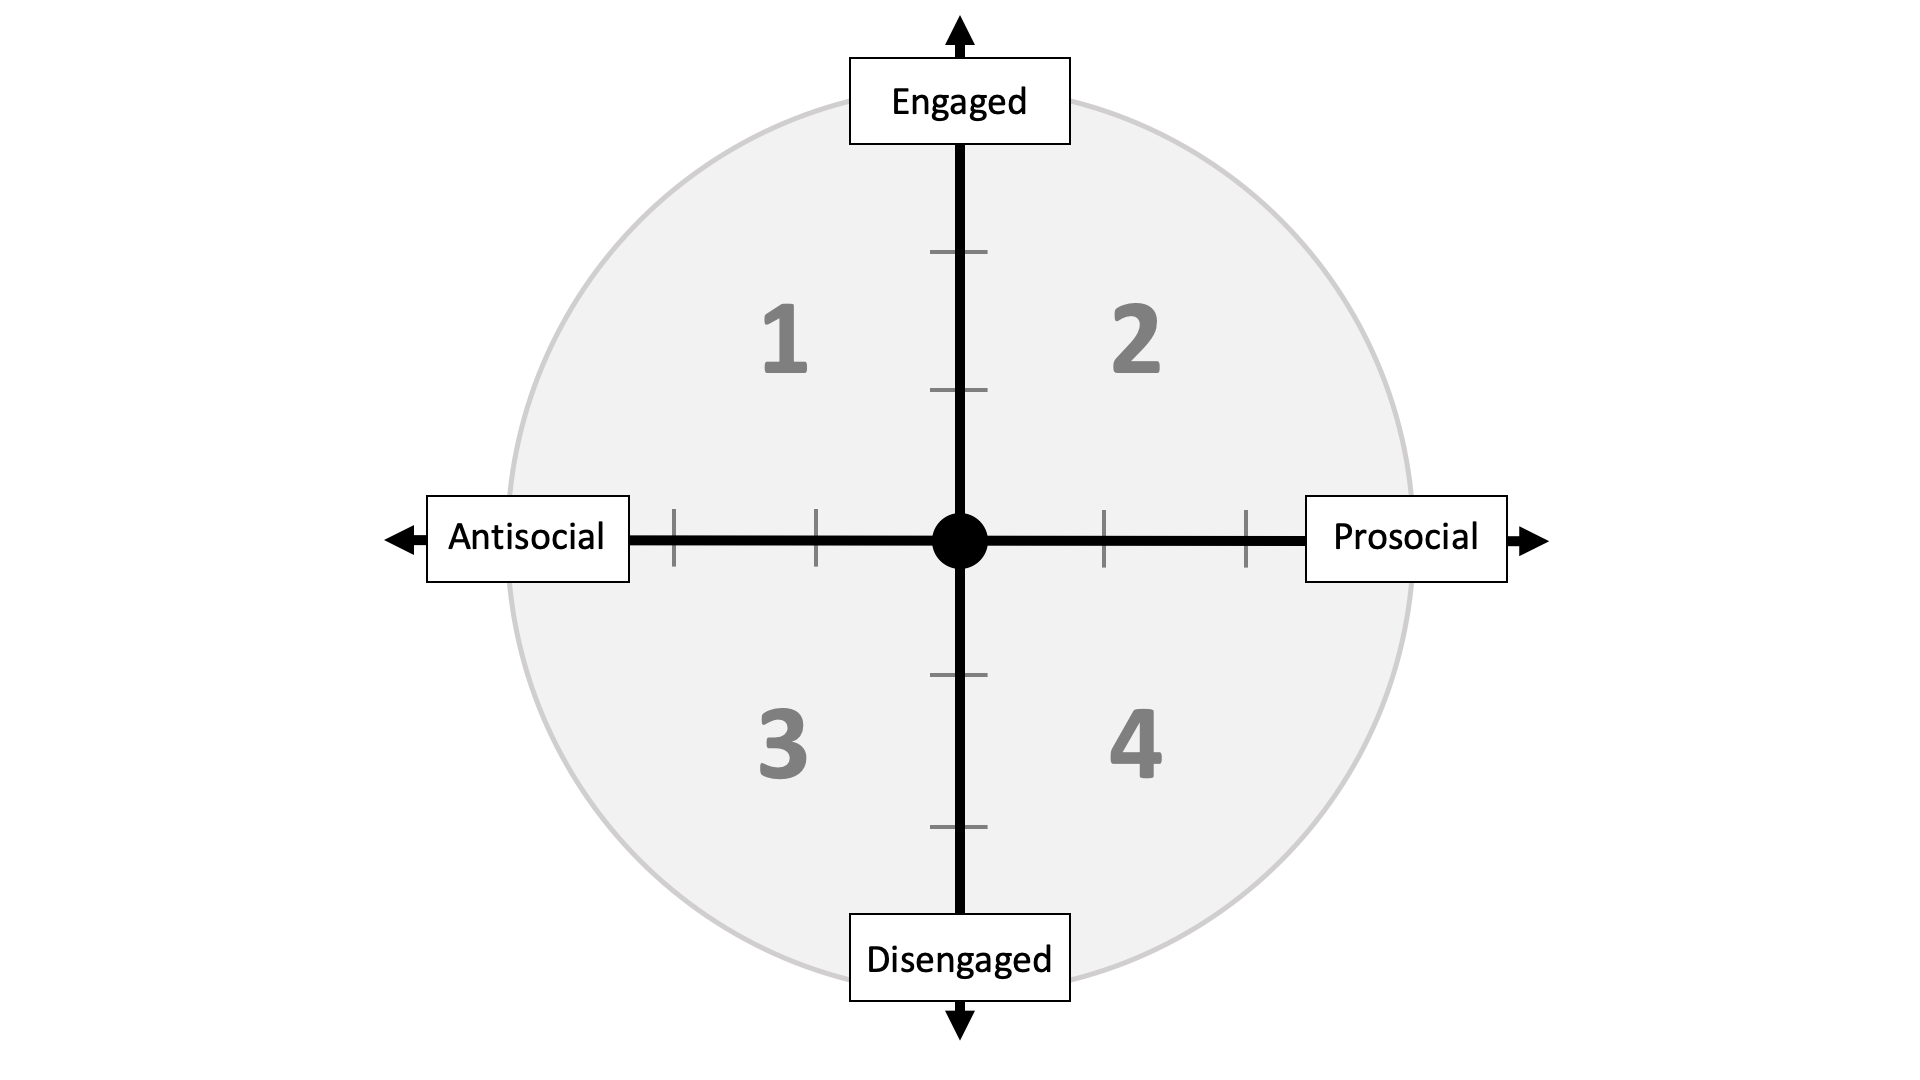
\includegraphics[width=1\linewidth]{images/bidr-all} \caption{Conceptual figure of the bi-dimensional rejection taxonomy. The antisocial--prosocial \emph{x}-axis refers to rejection responses that function to reduce (antisocial) or promote (prosocial) social connection. The engaged--disengaged \emph{y}-axis represents engaged (direct, active, ``hands-on'', approach-based) and disengaged (indirect, passive, ``hands-off'', avoidance-based) attempts to cope with the stressor (the current or future need-threat elicited by the rejection experience). The numbers in the figure represent quadrants: Quadrant 1 (engaged antisocial responses), Quadrant 2 (engaged prosocial responses), Quadrant 3 (disengaged antisocial responses), and Quadrant 4 (disengaged prosocial responses).}\label{fig:bidr-all}
\end{figure}

Our new taxonomy benefits the rejection literature in three ways. First,
it provides a unified map for researchers to organize belonging-relevant
responses to interpersonal rejection. Without this map, researchers
would solely rely on the antisocial--prosocial \emph{x}-axis, leading to
inaccurate conclusions about rejection-elicited responses, as
highlighted throughout the paper. For example, if a researcher only
assessed engaged prosocial responses to rejection, and rejected
participants didn't preferentially display these responses, the
researcher might erroneously conclude that rejection doesn't lead to
prosocial responses at all. Using the bi-dimensional rejection taxonomy,
we can see that rejected participants could still display prosocial
behavior, but in a disengaged manner. Thus, the engaged--disengaged
\emph{y}-axis of the bi-dimensional rejection taxonomy creates a cohesive
framework, preventing researchers from reaching inaccurate conclusions
about rejection-elicited responses.

Second, having a bi-dimensional framework allows researchers to generate
more nuanced and accurate predictions about responses to rejection. In
the past, researchers focused exclusively on how rejection affected
antisocial and prosocial behavior (the \emph{x}-axis) without differentiating
types of behavior within these categories. As a result, existing
hypotheses were limited in specificity. With the bi-dimensional
rejection taxonomy, researchers can generate more nuanced and innovative
hypotheses that incorporate both the antisocial--prosocial \emph{x}-axis and
the engaged--disengaged \emph{y}-axis. For example, without the taxonomy, a
researcher might hypothesize that both Situation A and Situation B lead
to prosocial responses following rejection. However, with the new
taxonomy, researchers can hypothesize that Situation A leads to engaged
prosocial responses (e.g., reaching out to close others for connection),
whereas Situation B leads to disengaged prosocial responses (e.g.,
watching their favorite TV program to feel socially connected). This
hypothesis highlights potential differences between Situation A and B
that would not be apparent without the taxonomy. Thus, the taxonomy arms
researchers with a comprehensive framework of potential response
options. Researchers can then use existing theoretical and empirical
work to generate more nuanced and accurate hypotheses.

Third, the bi-dimensional rejection taxonomy highlights types of
responses that are understudied in the rejection literature. As we
discuss later, the bulk of rejection research has focused on engaged
antisocial and prosocial responses. Using the lens of the bi-dimensional
rejection taxonomy, we can see that many disengaged responses are yet to
be examined in the context of rejection, highlighting the need for
further research.

In proposing the taxonomy, we rely on existing work demonstrating that
self-protective and belonging needs are fundamental to human nature, and
that interpersonal rejection threatens these needs, motivating
behavioral responses (\citeproc{ref-baumeisterNeedBelongDesire1995}{Baumeister \& Leary, 1995}; \citeproc{ref-maslow1943}{Maslow, 1943}; \citeproc{ref-murrayBalancingConnectednessSelfprotection2008}{Murray et al., 2008}; \citeproc{ref-richmanReactionsDiscriminationStigmatization2009}{Richman \& Leary, 2009}; \citeproc{ref-williamsOstracismTemporalNeedthreat2009}{Williams, 2009}). Throughout this paper, we use
interpersonal rejection as an overarching phrase that encompasses
threats to belonging, including social exclusion, social rejection,
ostracism, and relational devaluation---referring to experiences when a
person feels like they aren't loved, cared for, or accepted
(\citeproc{ref-learySelfesteemInterpersonalMonitor1995}{Leary et al., 1995}). \footnote{While being denied a desired opportunity (e.g., employment,
  publication, etc.) is commonly referred to as rejection in lay
  terms, those types of experiences are outside the scope of this
  paper because they are not forms of interpersonal rejection; they do
  not convey to a person that they are uncared for or unloved.
  Similarly, intergroup rejection (a group excluded by a group) is
  outside the scope of this paper.}

We exclusively focus on responses to rejection that are purposeful and
voluntary (in contrast to automatic and involuntary responses) since our
goal is to describe how people cope with rejection. This focus is
consistent with the coping literature (on which the \emph{y}-axis is heavily
based) that defines coping as purposeful and conscious attempts to deal
with the stressor (\citeproc{ref-connor-smithResponsesStressAdolescence2000}{Connor-Smith et al., 2000}).
Automatic or involuntary responses (e.g., attentional bias to smiling
faces) are outside the scope of the taxonomy and thus outside the scope
of this paper.

We divide the current paper into two parts. In the first half, we review
previous research supporting the antisocial--prosocial \emph{x}-axis and
introduce a novel engaged--disengaged \emph{y}-axis. In the second half, we
highlight how the taxonomy allows researchers to see existing published
work through a new lens and discuss new directions for future research.

\section{\texorpdfstring{Existing Dimension: The Antisocial--Prosocial \emph{x}-Axis}{Existing Dimension: The Antisocial--Prosocial x-Axis}}\label{existing-dimension-the-antisocialprosocial-x-axis}

In this section, we review existing empirical and theoretical literature
supporting the antisocial-prosocial \emph{x}-axis. This dimension has been
discussed extensively elsewhere (e.g., \citeproc{ref-murrayOptimizingAssuranceRisk2006}{Murray et al., 2006}; \citeproc{ref-richmanReactionsDiscriminationStigmatization2009}{Richman \& Leary, 2009}; \citeproc{ref-williamsOstracismTemporalNeedthreat2009}{Williams, 2009}). Accordingly, we briefly highlight relevant work on
interpersonal rejection and close relationships to support our use of
the antisocial-prosocial \emph{x}-axis. We discuss the novel
engaged--disengaged \emph{y}-axis in the next section.

\subsection{Foundational Theories in the Rejection Literature}\label{foundational-theories-in-the-rejection-literature}

The antisocial--prosocial \emph{x}-axis of the bi-dimensional rejection
taxonomy stems from prior empirical research demonstrating that
rejection sometimes leads to antisocial behavior and, at other times,
prosocial behavior (\citeproc{ref-dewall2009}{DeWall et al., 2009}, \citeproc{ref-dewallLittleAcceptanceGoes2010}{2010}; \citeproc{ref-romero-canyasPayingBelongWhen2010}{Romero-Canyas et al., 2010}; \citeproc{ref-twengeIfYouCan2001}{Twenge et al., 2001}; \citeproc{ref-warburtonWhenOstracismLeads2006}{Warburton et al., 2006}). For
example, rejected participants blasted louder and longer noise to a
stranger in one study {[}an antisocial response; Twenge et al. (\citeproc{ref-twengeIfYouCan2001}{2001}){]} and worked
harder on a collective task in another study {[}a prosocial response;
Williams \& Sommer (\citeproc{ref-williams1997}{1997}){]} compared with non-rejected participants. Rejection
scholars have developed multiple theoretical frameworks for
understanding these interpersonal responses to rejection that fall along
the antisocial-prosocial \emph{x}-axis. We refer readers to other theoretical
papers for more extensive discussions of this dimension (\citeproc{ref-richmanReactionsDiscriminationStigmatization2009}{Richman \& Leary, 2009}; \citeproc{ref-williamsOstracismTemporalNeedthreat2009}{Williams, 2009}) and summarize relevant theories here to support the
antisocial-prosocial \emph{x}-axis of the bi-dimensional rejection taxonomy.

Many previous theories commonly highlight the existence of the
antisocial--prosocial \emph{x}-axis. For example, the multimotive model
defines antisocial responses as those that function to diminish
belonging whereas prosocial responses as those that function to enhance
belonging (\citeproc{ref-richmanReactionsDiscriminationStigmatization2009}{Richman \& Leary, 2009}). The need-threat model also identifies
aggression (antisocial responses) and prosocial responses as primary
categories of responses to cope with interpersonal rejection
(\citeproc{ref-williamsOstracismTemporalNeedthreat2009}{Williams, 2009}). Similarly, the reconnection hypothesis and the resource
redistribution model both agree that responses to rejection range in
function from antisocial to prosocial (\citeproc{ref-dewall2011}{DeWall \& Richman, 2011}; \citeproc{ref-shilling2015}{Shilling \& Brown, 2015}).
These theories all agree that motives to self-protect or regain control
predict antisocial responses, and motives to obtain belonging predict
prosocial responses (\citeproc{ref-dewall2011}{DeWall \& Richman, 2011}; \citeproc{ref-shilling2015}{Shilling \& Brown, 2015}; \citeproc{ref-williamsOstracismTemporalNeedthreat2009}{Williams, 2009}). In sum,
rejection theories strongly support the existence of the
antisocial--prosocial dimension.

\subsection{Foundational Theories in the Close Relationships Literature}\label{foundational-theories-in-the-close-relationships-literature}

Close relationships researchers also support the existence of an
antisocial-prosocial \emph{x}-axis. For instance, the investment model
suggests that responses to relationship decline within a romantic
relationship (a form of perceived rejection) can range from destructive
(e.g., relationship-damaging responses such as leaving the relationship;
similar to antisocial behavior) to constructive {[}e.g.,
relationship-repairing responses such as voicing a concern; similar to
prosocial behavior; Rusbult et al. (\citeproc{ref-rusbultExitVoiceLoyalty1982}{1982}){]}. Similarly, risk regulation theory
suggests that couples' responses towards each other function to promote
or damage the relationships (\citeproc{ref-murrayOptimizingAssuranceRisk2006}{Murray et al., 2006}), akin to antisocial and
prosocial behavior within the romantic relationship.

The rapid marital coding system (RMICS) also supports the existence of
the antisocial-prosocial \emph{x}-axis. The RMICS describes behaviors that
partners display towards each other on a continuum ranging from
hostility to positivity (\citeproc{ref-heyman2004}{Heyman, 2004}). On the left end of the continuum,
hostile responses function to reduce connection between partners,
similar to antisocial responses. On the right side of the continuum,
positive responses function to increase connection between partners,
similar to prosocial responses.

These close relationships theories strongly support the existence of the
antisocial--prosocial \emph{x}-axis. This dimension has been identified in
different terms: destructive--constructive in the investment model
(\citeproc{ref-rusbultExitVoiceLoyalty1982}{Rusbult et al., 1982}), self-protection--relationship promotion in risk
regulation theory (\citeproc{ref-murrayOptimizingAssuranceRisk2006}{Murray et al., 2006}), and hostilit\emph{y}--positivity in the
RMICS (\citeproc{ref-heyman2004}{Heyman, 2004}). However, all of the terms reflect the same
underlying concept of behaviors that reduce (antisocial) or increase
(prosocial) connection with others. In addition, similar to the
rejection literature, risk regulation theory argues that antisocial
behaviors are motivated by self-protection concerns whereas prosocial
responses are motivated by belonging needs (\citeproc{ref-murrayOptimizingAssuranceRisk2006}{Murray et al., 2006}).

\subsection{Defining Antisocial and Prosocial Responses}\label{defining-antisocial-and-prosocial-responses}

As discussed above, multiple theories in the rejection and close
relationships literatures strongly support an antisocial--prosocial
dimension for understanding interpersonal responses to rejection. This
consensus provides a strong foundation for the \emph{x}-axis in the
bi-dimensional rejection taxonomy. All theories consistently discuss how
antisocial responses function to reduce social connection between the
self and others, motivated by self-protection needs, and how prosocial
responses function to promote social connection, motivated by belonging
needs. Accordingly, we adopt these definitions in the bi-dimensional
rejection taxonomy. Telling someone ``I hate you'' would thus be an
antisocial response because it functions to reduce social connection
with the other person. On the other hand, telling someone ``I love you''
would be a prosocial response because it functions to promote social
connection.

Note that the word prosocial is sometimes used to denote altruistic
behaviors that benefit the welfare of others---these behaviors may or
may not function to promote connection with others
(\citeproc{ref-batsonAltruismProsocialBehavior2003}{Batson \& Powell, 2003}). In this paper, we use the label
prosocial to refer to behaviors that promote social connection with
others, consistent with typical uses of the word in rejection research
(\citeproc{ref-blackhartRejectionImpactSelfdefeating2006}{Blackhart et al., 2006}; \citeproc{ref-richmanReactionsDiscriminationStigmatization2009}{Richman \& Leary, 2009}; \citeproc{ref-williamsReactingOstracismRetaliation2005}{Williams \& Govan, 2005}).

\section{\texorpdfstring{A New Dimension: The Engaged--Disengaged \emph{y}-Axis}{A New Dimension: The Engaged--Disengaged y-Axis}}\label{a-new-dimension-the-engageddisengaged-y-axis}

A close inspection of existing empirical work reveals that there is
significant variability within antisocial and prosocial
responses---reflecting heterogeneous strategies for responding to
interpersonal rejection. For example, prior research demonstrated that
rejection sometimes leads to direct and active attempts to connect with
others {[}e.g., spending money to garner acceptance from others;
Maner et al. (\citeproc{ref-manerDoesSocialExclusion2007}{2007}); Romero-Canyas et al. (\citeproc{ref-romero-canyasPayingBelongWhen2010}{2010}){]}. At
other times, rejection leads to indirect and passive attempts to connect
with others {[}e.g., experiencing nostalgia;
Derrick et al. (\citeproc{ref-derrickSocialSurrogacyHow2009}{2009}){]}. No existing theories of interpersonal
rejection can distinguish between these varied responses---both types of
responses are categorized as prosocial in the context of existing
theories. The bi-dimensional rejection taxonomy makes a novel claim that
the antisocial--prosocial \emph{x}-axis captures only one dimension of
responses, and that a new dimension is needed to fully understand
responses to rejection. In this section, we first review foundational
theories that suggest an additional possible dimension. Then, we define
our new engaged--disengaged \emph{y}-axis at the end of this section.

\subsection{Foundational Theories}\label{foundational-theories}

To understand the variation within antisocial and prosocial responses,
we rely on theoretical and empirical work in the coping literature. This
extensive literature describes the ways in which people cope with (i.e.,
voluntarily and purposefully respond to) stressors; thus, this
literature provides a rich foundation for building our \emph{y}-axis.

Coping researchers have proposed various ways to classify coping
responses, including emotion-focused, problem-focused, proactive, and
meaning-focused coping (\citeproc{ref-aspinwallStitchTimeSelfregulation1997}{Aspinwall \& Taylor, 1997}; \citeproc{ref-lazarusStressAppraisalCoping1984}{R. S. Lazarus \& Folkman, 1984}; \citeproc{ref-skinnerSearchingStructureCoping2003}{Skinner et al., 2003}). Using factor analyses and
theoretical discussions, researchers identified an engaged--disengaged
dimension as the critical factor underlying the majority of coping
responses (\citeproc{ref-carverPersonalityCoping2010}{Carver \& Connor-Smith, 2010}; \citeproc{ref-compasEffortfulInvoluntaryResponses1997}{Compas et al., 1997}; \citeproc{ref-connor-smithResponsesStressAdolescence2000}{Connor-Smith et al., 2000}; \citeproc{ref-dijkstraEngagingRatherDisengaging2016}{Dijkstra \& Homan, 2016}; \citeproc{ref-scheierCopingStressDivergent1986}{Scheier et al., 1986}; \citeproc{ref-skinnerSearchingStructureCoping2003}{Skinner et al., 2003}; \citeproc{ref-tobinHierarchicalFactorStructure1989}{Tobin et al., 1989}). According to this literature,
engaged coping strategies are direct and active behaviors that confront
the stressor with a ``hands-on'' approach. A person has used an engaged
coping strategy when they act out their frustrations on others (e.g.,
aggression), seek social support, or behave in other active and direct
ways (\citeproc{ref-carverPersonalityCoping2010}{Carver \& Connor-Smith, 2010}; \citeproc{ref-dijkstraEngagingRatherDisengaging2016}{Dijkstra \& Homan, 2016}). On the other hand, disengaged
coping strategies refer to indirect and passive behaviors that aim to
avoid the stressor. Examples of disengaged coping are social withdrawal,
denial, and wishful thinking (\citeproc{ref-carverPersonalityCoping2010}{Carver \& Connor-Smith, 2010}).

We can easily apply the distinction between engaged and disengaged
coping to understand how people respond to interpersonal rejection. In
the context of rejection, the stressor that people are coping with is
the threat to belonging and self-protection/control experienced by the
rejected person. As noted earlier, these need-threats are
well-documented consequences of experiencing rejection
(\citeproc{ref-williamsOstracismTemporalNeedthreat2009}{Williams, 2009}). The threats to belonging or
self-protection/control can be present-oriented, when a person is trying
to cope with the current need-threat, or it can be future-oriented, when
a person is trying to pre-emptively cope with a potential future
need-threat. In coping with those stressors, people can respond in ways
that are more engaged versus disengaged. We adopt these ideas in
defining the \emph{y}-axis, as described in the next section.

Although no past theories have explicitly differentiated responses to
rejection as engaged or disengaged, some researchers have implied the
existence of this distinction by separating social withdrawal from other
antisocial responses. For example, the multimotive model identifies
social withdrawal as a subtype of antisocial (belonging-diminishing)
responses that are separate from more overt antisocial responses such as
aggression (\citeproc{ref-richmanReactionsDiscriminationStigmatization2009}{Richman \& Leary, 2009}).
Attachment theory also differentiated social withdrawal from other overt
forms of behavior (e.g., aggression) as a response to prolonged
rejection from an attachment figure (\citeproc{ref-bowlbySeparationAnxietyAnger2000}{Bowlby, 2000}; \citeproc{ref-horneyNeuroticPersonalityOur1964}{Horney, 1964}). These theories both support the
distinction proposed by the coping literature: disengaged antisocial
responses are different from engaged antisocial responses. As we
describe later, a benefit of formally defining the engaged--disengaged
\emph{y}-axis is that it highlights additional forms of disengaged antisocial
responses that have been neglected by existing theories.

Another theory that supports differentiating antisocial and prosocial
responses is the investment model, a widel\emph{y}-used theoretical model in
the romantic relationships literature. The investment model uses a
two-dimensional space, characterizing how romantic partners behave when
their romantic relationship is in decline (\citeproc{ref-rusbultExitVoiceLoyalty1982}{Rusbult et al., 1982}; \citeproc{ref-rusbultResponsesDissatisfactionClose1987}{Rusbult, 1987}; \citeproc{ref-rusbultInterdependenceAnalysisAccommodation1991}{Rusbult \& Verette, 1991}). Specifically, the investment
model proposes the destructive--constructive dimension (similar to our
antisocial--prosocial \emph{x}-axis, as described previously) and the
active--passive dimension (similar to, but also different from, our
engaged--disengaged \emph{y}-axis). Before discussing similarities and
differences between the multimotive model, the investment model, and our
new taxonomy, we first define the disengaged--engaged \emph{y}-axis so that
the reader has a complete understanding of these terms. Then, in the
following section, we discuss how our model contributes over and above
existing work in advancing our understanding of responses to
interpersonal rejection.

\subsection{Defining Engaged--Disengaged Responses to Rejection}\label{defining-engageddisengaged-responses-to-rejection}

Based on the literature reviewed above, we propose the
engaged--disengaged \emph{y}-axis that describes whether a response to
rejection represents an engaged or disengaged attempt to cope with the
stressor. Again, the stressor in the context of rejection is the current
or future need-threat {[}i.e., the threat to self-protection/control or
affiliation needs; Baumeister \& Leary (\citeproc{ref-baumeisterNeedBelongDesire1995}{1995});
Williams (\citeproc{ref-williamsOstracismTemporalNeedthreat2009}{2009}){]}. We define engaged responses
as direct and active attempts to deal with the stressor. They are
``hands-on'', approach-based strategies to confront and face the stressor.
An example of an engaged antisocial response is behaving aggressively
towards one's romantic partner, because exerting control over one's
partner actively and directly replenishes the sense of
self-protection/control thwarted by rejection. An example of an engaged
prosocial response is seeking support from a loved one because this
response actively and directly replenishes the sense of belonging
thwarted by rejection (\citeproc{ref-murrayWhenRejectionStings2002}{Murray et al., 2002}, \citeproc{ref-murrayBalancingConnectednessSelfprotection2008}{2008}).

In contrast, we define disengaged responses as indirect and passive
attempts to handle the stressor. They are ``hands-off'', avoidance-based
strategies to evade and divert from the stressor. These responses help
to avoid threats to belonging or self-protection/control. An example of
a disengaged antisocial response is social withdrawal, because
withdrawing is a hands-off strategy that allows a person to avoid
further rejection (and thus further threats to belonging or
self-protection/control). An example of a disengaged prosocial response
is relying on social surrogates (e.g., parasocial relationships)---such
as watching one's favorite TV show or passively browsing social media to
obtain social connection. This qualifies as disengaged because social
surrogates allow people to passively and indirectly replenish belonging
while avoiding future rejection.

Importantly, the engaged--disengaged \emph{y}-axis is defined by whether the
response itself is engaged (direct, active, hands-on) or disengaged
(indirect, passive, hands-off); it is not defined by the situation or
environment in which it occurs. At the same time, recognizing the
situation in which the response occurs is important because the
situation limits possible response options. In a person's da\emph{y}-to-day
life, there is often a lot of flexibility in responding. For example, a
rejected person can choose whether to seek social support (an engaged
response) or watch their favorite TV show (a disengaged response) even
if they are in the same situation (e.g., at home with their romantic
partner on a Friday after work). This response flexibility is usually
absent among lab studies where participants are given only one option to
respond (e.g., participating in a noise blast task and deciding how much
noise to blast, but not being given any other response options). Thus,
the situation has the potential to constrain responses to be either
engaged or disengaged, especially in laboratory studies. Using the
engaged--disengaged \emph{y}-axis, researchers can design studies that
include diverse response options, as we highlight in the future
directions section towards the end of the paper.

Together with the antisocial--prosocial \emph{x}-axis, the
engaged--disengaged \emph{y}-axis completes the bi-dimensional rejection
taxonomy. These two dimensions both describe the function of a given
response: whether a response functions to reduce or promote connection
(\emph{x}-axis) and whether a response functions as a direct, active,
hands-on way of coping versus an indirect, passive, hands-off way of
coping with the stressor (\emph{y}-axis). In the next section, we discuss how
the bi-dimensional rejection taxonomy compares with the existing
theories of social behavior. Then, we provide examples of responses
within each quadrant, demonstrating how the two dimensions are
independent from each other.

\section{Comparisons with Existing Theories}\label{comparisons-with-existing-theories}

The bi-dimensional rejection taxonomy provides a novel lens through
which to view responses to rejection, incorporating both the
antisocial--prosocial and engaged--disengaged dimensions. How does the
taxonomy compare with other theories? In this section, we discuss the
advantages of the bi-dimensional rejection taxonomy over existing
theories in the rejection and close relationships literatures.

Compared with existing rejection theories, the bi-dimensional rejection
taxonomy provides a more nuanced and accurate depiction of responses to
interpersonal rejection. The main advantage of the taxonomy is its power
to differentiate engaged and disengaged responses, particularly
prosocial responses. Past literature showed that rejected people respond
in ways that qualify as disengaged and prosocial, such as thinking about
one's favorite TV program (e.g., \citeproc{ref-derrickSocialSurrogacyHow2009}{Derrick et al., 2009}) and
that people can fulfill belonging in a variety of ways, including via
social surrogates {[}e.g., a fictional character; Gabriel \& Valenti (\citeproc{ref-gabrielSocialSurrogatesRejection2017}{2017}){]}. However, no existing theories have formally differentiated these
types of prosocial responses from other more engaged responses (e.g.,
seeking social support from a loved one; Murray et al., 2008). The
bi-dimensional rejection taxonomy also differentiates disengaged
antisocial responses. Among disengaged responses, social withdrawal is
the only form of disengaged antisocial responses currently described by
existing rejection theories, such as the multimotive model
(\citeproc{ref-richmanReactionsDiscriminationStigmatization2009}{Richman \& Leary, 2009}). With the current
taxonomy, we can see that there are additional types of disengaged
antisocial responses not described by the multimotive model or any other
existing theory (e.g., passive aggressive behavior, as we describe in
detail later). The bi-dimensional rejection taxonomy thus accounts for
more responses than any other framework available in the rejection
literature.

The bi-dimensional rejection taxonomy also offers advantages over the
investment model in the close relationships literature. The investment
model suggests that responses to romantic relationship decline range
along a two-dimensional space: the destructive--constructive (i.e., how
a response damages or nurtures the romantic relationship) and
active--passive (i.e., how a response overtly or indirectly affects the
romantic relationship) dimensions (\citeproc{ref-rusbultExitVoiceLoyalty1982}{Rusbult et al., 1982}). On the
surface, the bi-dimensional rejection taxonomy seems similar to the
investment model. However, the bi-dimensional rejection taxonomy is more
advantageous than the investment model in considering broader sources of
rejection and targets of the response. The investment model
characterizes situations when the romantic relationship partner is the
source of relationship decline, and it only characterizes responses
towards an existing relationship partner (\citeproc{ref-rusbultExitVoiceLoyalty1982}{Rusbult et al., 1982}).
The bi-dimensional rejection taxonomy captures threats to belonging from
any source while also characterizing responses towards any target, not
just the romantic partner. Finally, the engaged-disengaged \emph{y}-axis of
the bi-dimensional rejection taxonomy more accurately captures variation
among antisocial and prosocial responses evident in the rejection
literature. Whereas saying ``I hate you'' to one's partner is a passive
response (on the bottom half of the \emph{y}-axis) according to the
investment model (\citeproc{ref-rusbultExitVoiceLoyalty1982}{Rusbult et al., 1982}), this behavior would
quality as engaged (on the top half of the \emph{y}-axis) according to the
bi-dimensional rejection taxonomy. The \emph{y}-axis of the taxonomy is
founded on decades of work in the coping literature
(\citeproc{ref-carverPersonalityCoping2010}{Carver \& Connor-Smith, 2010}; \citeproc{ref-compasEffortfulInvoluntaryResponses1997}{Compas et al., 1997}; \citeproc{ref-connor-smithResponsesStressAdolescence2000}{Connor-Smith et al., 2000}; \citeproc{ref-dijkstraEngagingRatherDisengaging2016}{Dijkstra \& Homan, 2016}; \citeproc{ref-scheierCopingStressDivergent1986}{Scheier et al., 1986}; \citeproc{ref-skinnerSearchingStructureCoping2003}{Skinner et al., 2003}; \citeproc{ref-tobinHierarchicalFactorStructure1989}{Tobin et al., 1989}), and is also consistent with the
way existing rejection research classifies responses
(\citeproc{ref-richmanReactionsDiscriminationStigmatization2009}{Richman \& Leary, 2009}).

\section{Plotting Existing Studies in a Bi-Dimensional Space}\label{plotting-existing-studies-in-a-bi-dimensional-space}

In the previous sections, we reviewed literature supporting the
antisocial--prosocial \emph{x}-axis and introduced the engaged-disengaged
\emph{y}-axis to the rejection literature. We also compared this taxonomy
with existing theories, and demonstrated that the taxonomy presents many
advantages. In this section, we discuss select evidence demonstrating
that interpersonal responses to rejection can be plotted in this
two-dimensional space, broadly categorized into four quadrants: engaged
antisocial responses (Quadrant 1), engaged prosocial responses (Quadrant
2), disengaged antisocial responses (Quadrant 3), and disengaged
prosocial responses (Quadrant 4). We present a hypothetical exemplar for
each dimension in \ref{fig:bidr-exemplars} to illustrate the
differences among quadrants and help the reader understand each
quadrant. We also discuss existing research that falls into each
quadrant in this section. Since no past studies included both of these
new dimensions in their studies, we infer which quadrant a response
falls into based on the properties of the response. We begin by
reviewing existing empirical work that falls into Quadrant 1, and then
move to Quadrants 2, 3, and 4.

The bi-dimensional rejection taxonomy highlights types of responses that
have been understudied in the literature (e.g., passive aggressive
behavior and nostalgia). To better illustrate these new kinds of
responses, we discuss multiple examples for Quadrants 3 and 4 (i.e.,
disengaged antisocial and prosocial responses). Since past literature
has extensively discussed responses in Quadrant 1 and Quadrant 2 (i.e.,
engaged antisocial and prosocial responses, as discussed above), we
highlight only one representative example for these quadrants.

\begin{figure}
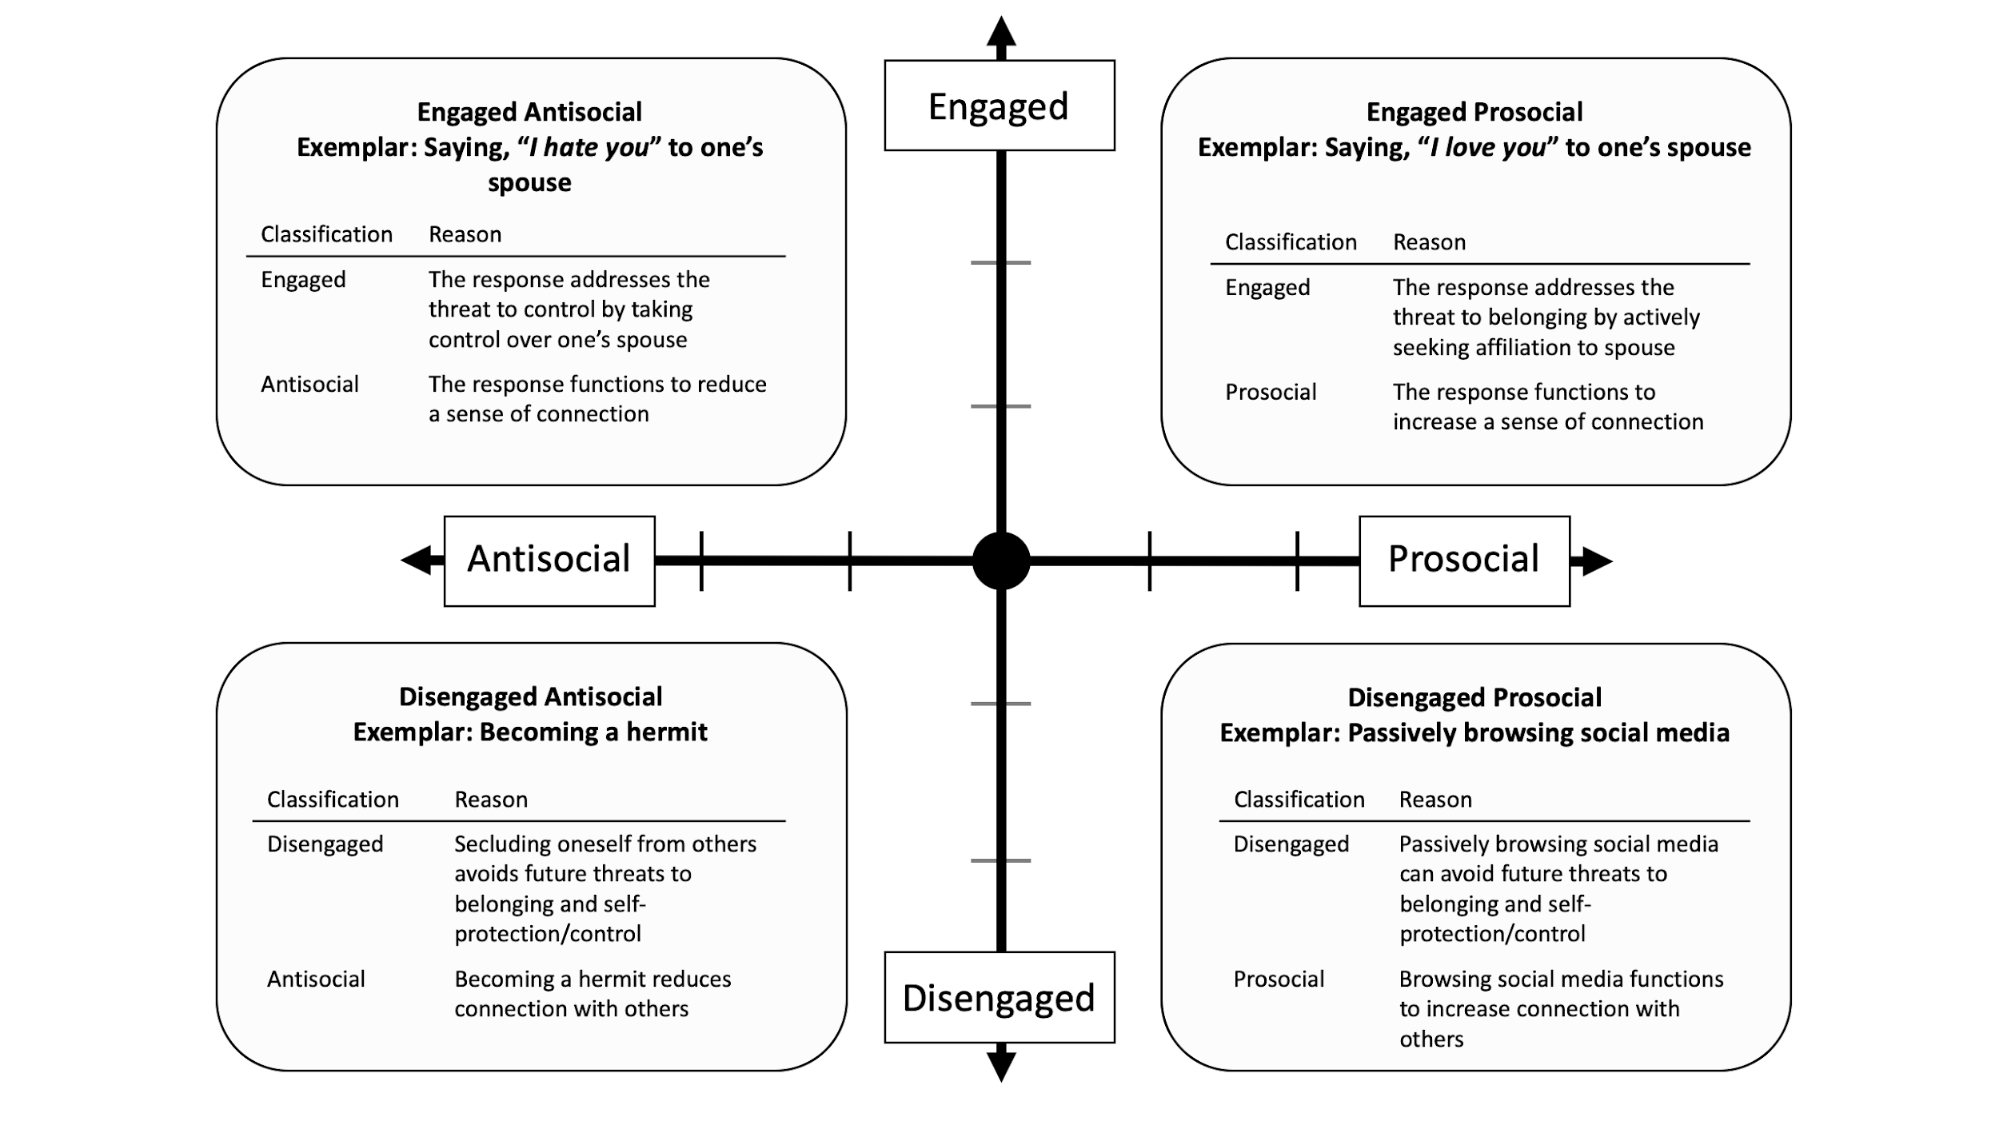
\includegraphics[width=1\linewidth]{images/bidr-exemplars} \caption{Summary of exemplar responses across quadrants. For each exemplar, we present reasons why we characterize them as antisocial versus prosocial and engaged versus disengaged.}\label{fig:bidr-exemplars}
\end{figure}

\subsection{Responses in Quadrant 1: Engaged Antisocial Responses}\label{responses-in-quadrant-1-engaged-antisocial-responses}

Past studies have demonstrated that rejected people respond in ways that
qualify as engaged and antisocial. For example, rejected people
allocated more hot sauce to a bystander who disliked spicy food,
compared with non-rejected people
(\citeproc{ref-aydukIndividualDifferencesRejection2008}{Ayduk et al., 2008}; \citeproc{ref-dewallLittleAcceptanceGoes2010}{DeWall et al., 2010}). This response is antisocial because it
functions to reduce connection with others
(\citeproc{ref-warburtonWhenOstracismLeads2006}{Warburton et al., 2006}; \citeproc{ref-williamsOstracismTemporalNeedthreat2009}{Williams, 2009}). It also qualifies as engaged
because it is a hands-on, approach-based and direct attempt to
re-establish threatened self-protection/control needs by exercising
dominance or control over others (\citeproc{ref-warburtonWhenOstracismLeads2006}{Warburton et al., 2006}).

\subsection{Responses in Quadrant 2: Engaged Prosocial Responses}\label{responses-in-quadrant-2-engaged-prosocial-responses}

Past studies showed that people seek their romantic partner's support
when faced with potential rejection from that partner, especially among
people with higher self-esteem
(\citeproc{ref-murrayWhenRejectionStings2002}{Murray et al., 2002}, \citeproc{ref-murrayBalancingConnectednessSelfprotection2008}{2008}). Applying our proposed taxonomy, we
suggest that this behavior qualifies as an engaged prosocial response
because seeking social support from a romantic partner functions to
increase social connection (a prosocial response) and actively confronts
the current threat to belonging by directly seeking social connection.

\subsection{Responses in Quadrant 3: Disengaged Antisocial Responses}\label{responses-in-quadrant-3-disengaged-antisocial-responses}

One advantage of the taxonomy is that it highlights disengaged
antisocial responses that are not accounted for by existing theories; we
discuss several examples within this quadrant. Compared with
non-rejected participants, rejected participants desired to withdraw
from subsequent social interactions (\citeproc{ref-renEvidenceAnotherResponse2015}{Ren et al., 2015}).
This response functions to reduce social connection by avoiding further
social contact. In light of our taxonomy, they are disengaged responses
because they avoid future threats to belonging and
self-protection/control by isolating oneself from others.

In addition to withdrawing socially, rejected people can structure their
environment to prevent social encounters. For instance, rejected people
preferred room configurations that hindered social interactions,
presumably to avoid interacting with other people
(\citeproc{ref-meagherSeekingSafetySociofugal2017}{Meagher \& Marsh, 2017}). This response is antisocial since
doing so reduces opportunities for social connection, and the response
is disengaged since it functions to evade future belonging threats.

Another example of a disengaged antisocial response is being
passive-aggressive by not engaging in a behavior that can prevent harm
to another person (\citeproc{ref-parrottAddressingCriterionProblem2007}{Parrott \& Giancola, 2007}; \citeproc{ref-southrichardsonEverydayAggressionTakes2014}{South Richardson, 2014}). For example, a rejected
person might intentionally not speak up to defend their partner when the
partner is insulted by others. This behavior is antisocial since doing
so reduces connection with the partner. It is also a disengaged response
since passive forms of aggression are ``hands-off'' and indirect means of
dealing with the stressor.

People who feel socially rejected are more prone to stop caring for
themselves by neglecting basic needs, a behavior called self-neglect,
another form of a disengaged antisocial response. Self-neglect refers to
inattention to personal hygiene and health (e.g., not showering or
wearing deodorant), often accompanied by behaviors such as hoarding and
refusal of help from others
(\citeproc{ref-abramsPredictorsSelfNeglectCommunityDwelling2002}{Abrams et al., 2002}; \citeproc{ref-dongCrosssectionalPopulationbasedStudy2010}{Dong et al., 2010}). People who engage in
self-neglecting behavior often report desires to avoid losing control
(\citeproc{ref-band-wintersteinElderSelfNeglect2012}{Band-Winterstein et al., 2012}; \citeproc{ref-bozinovskiOlderSelfNeglectersInterpersonal2000}{Bozinovski, 2000}). Thus, self-neglect is
a disengaged antisocial response because neglecting one's hygiene or
habitat functions to reduce social connection with others, and it is an
indirect and passive way to avoid future threat to
self-protection/control needs.

\subsection{Responses in Quadrant 4: Disengaged Prosocial Responses}\label{responses-in-quadrant-4-disengaged-prosocial-responses}

Many disengaged prosocial responses involve the use of social
surrogates---human or non-human targets with a psychological, but not
physical, connection (\citeproc{ref-gabrielSocialSurrogatesSocial2016}{Gabriel et al., 2016}; \citeproc{ref-gabrielSocialSurrogatesRejection2017}{Gabriel \& Valenti, 2017}). People turn to social surrogates to
obtain belonging (\citeproc{ref-gabrielSocialSurrogatesSocial2016}{Gabriel et al., 2016}; \citeproc{ref-gabrielSocialSurrogatesRejection2017}{Gabriel \& Valenti, 2017}). For example, remembering a fight
with a close other (i.e., perceived rejection) led people to think
longer about their favorite TV program (vs.~a non-favorite TV program),
interpreted as a prosocial attempt to restore belonging
(\citeproc{ref-derrickSocialSurrogacyHow2009}{Derrick et al., 2009}). The bi-dimensional rejection taxonomy
regards this response as disengaged and prosocial, since relying on
social surrogates helps people passively avoid future threats to
belonging or control while simultaneously increasing perceived
connection with others.

Another disengaged prosocial response is experiencing nostalgia---a
sentimental yearning for the past and memories of social connections
(\citeproc{ref-abeytaLookingBackMove2015}{Abeyta et al., 2015}; \citeproc{ref-wildschutNostalgiaRepositorySocial2010}{Wildschut et al., 2010}).
Rejected participants experienced more nostalgia compared with accepted
participants (\citeproc{ref-wildschutNostalgiaRepositorySocial2010}{Wildschut et al., 2010}). Nostalgia is a
disengaged prosocial response because it functions to increase perceived
social connection with other people, but it does so in a hands-off way
that allows people to avoid additional threats to belonging or
self-control.

Taken together, responses to interpersonal rejection can be placed into
the four quadrants of the bi-dimensional rejection taxonomy. Recognizing
these quadrants is important in planning and conducting studies. For
example, if a researcher provides engaged antisocial response options
and finds that rejected participants do not behave more antisocially
than included participants, they may incorrectly conclude that rejection
does not lead to antisocial responses. This conclusion may be inaccurate
because rejected participants may have instead used disengaged
antisocial responses if they were provided with the option to do so.
Researchers who incorporate the bi-dimensional rejection taxonomy can
avoid faulty conclusions and reach a more calibrated interpretation of
their findings.

\section{Using the Bi-Dimensional Rejection Taxonomy to Frame Existing Research}\label{using-the-bi-dimensional-rejection-taxonomy-to-frame-existing-research}

The bi-dimensional rejection taxonomy provides researchers with a more
nuanced and accurate understanding of responses to rejection.
Previously, researchers were constrained to conclude that certain
individual difference or situational factors caused either antisocial or
prosocial behavior following rejection, without the appropriate language
for specifying the type of antisocial or prosocial behavior being
displayed. In this section, we view past research within the new lens of
the taxonomy to look for individual differences and situational factors
that appear to predict variation along the engaged--disengaged \emph{y}-axis.
In doing so, we make inferences about the \emph{y}-axis post-hoc based on the
available evidence, since the \emph{y}-axis was not a part of the lexicon at
the time those studies were conducted. We omit factors exclusively
predicting variation along the antisocial--prosocial \emph{x}-axis, such as
need fortification (e.g., \citeproc{ref-williamsOstracismTemporalNeedthreat2009}{Williams, 2009}),
because they have been extensively discussed elsewhere
(\citeproc{ref-learyInterpersonalRejectionDeterminant2006}{Leary et al., 2006}; \citeproc{ref-richmanReactionsDiscriminationStigmatization2009}{Richman \& Leary, 2009}; \citeproc{ref-williamsOstracismTemporalNeedthreat2009}{Williams, 2009}). We divide this section into
two parts. The first part focuses on variation in engaged and disengaged
antisocial responses, and the second focuses on variation in engaged and
disengaged prosocial responses.

\subsection{Factors Predicting Engaged versus Disengaged Antisocial Responses (Figure \ref{fig:bidr-antisocial})}\label{factors-predicting-engaged-versus-disengaged-antisocial-responses-figure-reffigbidr-antisocial}

\begin{figure}
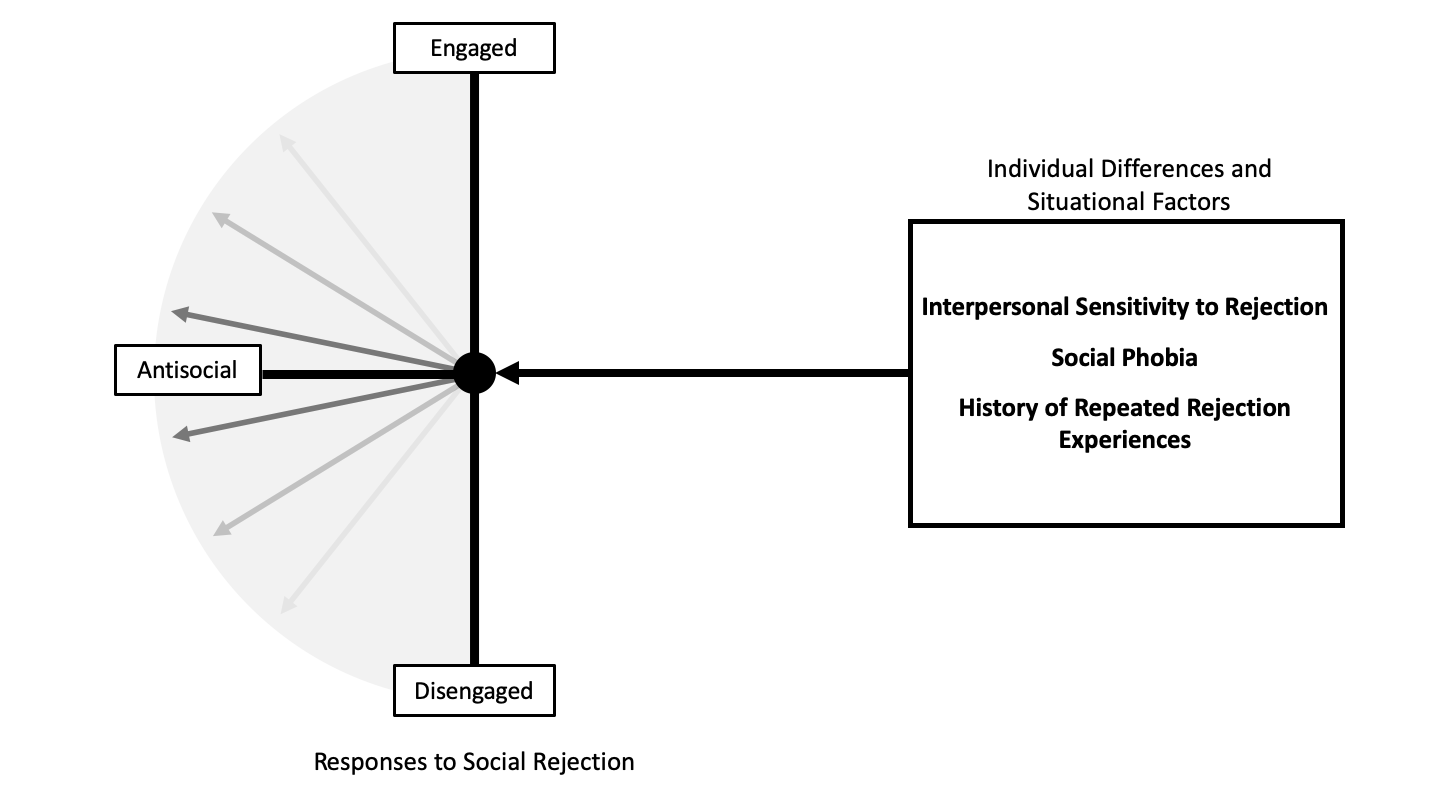
\includegraphics[width=1\linewidth]{images/bidr-antisocial} \caption{Representative individual differences and situational factors predicting engaged and disengaged antisocial responses. For illustrative purposes, only the antisocial hemisphere is depicted in this diagram. Higher interpersonal sensitivity to rejection (assessed via rejection sensitivity or low self-esteem) predicts engaged antisocial responses. Social phobia and history of repeated prior rejection experiences predict disengaged antisocial responses.}\label{fig:bidr-antisocial}
\end{figure}

\textbf{Interpersonal Sensitivity to Rejection (Rejection Sensitivity and
Self-Esteem).} Some people worry about being rejected more than others.
This tendency is present among people with higher rejection sensitivity
and lower self-esteem (\citeproc{ref-downeyImplicationsRejectionSensitivity1996}{Downey \& Feldman, 1996}; \citeproc{ref-feldmanRejectionSensitivityMediator1994}{Feldman \& Downey, 1994}; \citeproc{ref-learySelfesteemInterpersonalMonitor1995}{Leary et al., 1995}). Although these constructs
have important differences, they share significant conceptual
underpinnings representing an overlapping construct, sensitivity to
rejection (\citeproc{ref-crockerCostlyPursuitSelfesteem2004}{Crocker \& Park, 2004}; \citeproc{ref-parkResponsesSelfthreatLinking2010}{Park, 2010}). For these reasons, we label this
construct as \emph{interpersonal sensitivity to rejection} and discuss the
construct in reference to both indices.

People with higher interpersonal sensitivity to rejection may be more
likely to use engaged antisocial responses rather than disengaged
antisocial responses (Figure \ref{fig:bidr-antisocial}). Specifically,
past evidence has demonstrated a consistent link between higher
interpersonal sensitivity and engaged antisocial behavior, such as
aggression (\citeproc{ref-aydukIndividualDifferencesRejection2008}{Ayduk et al., 2008}; \citeproc{ref-downeyRejectionSensitivityChildren1998}{Downey, Lebolt, et al., 1998}; \citeproc{ref-downeySelffulfillingProphecyClose1998}{Downey, Freitas, et al., 1998}; \citeproc{ref-downeyRejectionSensitivityMale2000}{Downey et al., 2000}; \citeproc{ref-murrayWhenRejectionStings2002}{Murray et al., 2002}).
A review of the rejection sensitivity literature concludes that people
high in rejection sensitivity respond to rejection in hostile and
overtly aggressive ways (\citeproc{ref-romero-canyasPayingBelongWhen2010}{Romero-Canyas et al., 2010}). Also,
following a romantic relationship threat, people with lower self-esteem
derogated their romantic partner as being more lazy and thoughtless
relative to those with higher self-esteem
(\citeproc{ref-murrayWhenRejectionStings2002}{Murray et al., 2002}). These engaged antisocial responses may
be the result of a self-fulfilling prophec\emph{y}---people fearfully
expecting rejection can act in ways that provoke rejection from others,
such as putting down their romantic partner during face-to-face
interactions or perpetrating intimate partner violence
(\citeproc{ref-downeySelffulfillingProphecyClose1998}{Downey, Freitas, et al., 1998}; \citeproc{ref-downeyRejectionSensitivityMale2000}{Downey et al., 2000}).

\textbf{Social Phobia.} While the literature reviewed above consistently
demonstrates that people with higher interpersonal sensitivity to
rejection behave in engaged antisocial ways following rejection, related
literature shows the opposite pattern. Specifically, people with a
social phobia, an extreme form of interpersonal sensitivity to
rejection, often behave in disengaged antisocial ways. For example,
people with a social phobia often ruminate about social interactions
without engaging in them and avoid interacting with people (and thus
potential rejection) at all costs
(\citeproc{ref-clarkCognitivePerspectiveSocial2001}{Clark, 2001}). In addition, people with a
social phobia tend to avoid eye contact and emotionally distance
themselves from others when experiencing interpersonal problems
(\citeproc{ref-aldenInterpersonalProcessesSocial2004}{Alden \& Taylor, 2004}). Thus, at least some forms of
interpersonal sensitivity to rejection, in this case social phobia,
actually predict disengaged rather than engaged antisocial responses.

These subtle differences highlight the importance of the bi-dimensional
rejection taxonomy. Without the taxonomy, researchers would conclude
that people who are highly sensitive to rejection (both in terms of
rejection sensitivity, low self-esteem, and social phobia) behave in
antisocial ways following rejection. Using the bi-dimensional rejection
taxonomy, we can see that the most extreme form of sensitivity to
rejection (social phobia) leads to disengaged antisocial behavior,
whereas other forms of sensitivity to rejection (e.g., low self-esteem)
lead to engaged antisocial behavior. Noticing this subtle yet important
difference in responses allows researchers to begin asking why a
difference exists. For example, armed with the bi-dimensional rejection
taxonomy, we could begin asking whether methodological differences could
explain why interpersonal sensitivity led to engaged versus disengaged
antisocial responses (e.g., did each study provide participants with
both engaged and disengaged antisocial response options?). We could also
begin wondering whether there is something qualitatively different
between a more extreme, clinical interpersonal sensitivity versus those
in the normative range. Without the bi-dimensional rejection taxonomy
that differentiates disengaged and engaged antisocial responses,
researchers wouldn't be able to ask these important questions. The
taxonomy thus sheds light on an existing gap in our knowledge, spurring
future research.

\textbf{History of Repeated Rejection Experiences.} Another related
literature about repeated rejection experiences also highlights the
importance of the bi-dimensional rejection taxonomy. People have
different histories of being rejected---some have experienced rejection
more often than others (e.g., students who were bullied vs.~those who
were not). A repeated history of rejection plays an important role in
promoting antisocial responses to rejection, as highlighted by existing
theories (\citeproc{ref-bowlbySeparationAnxietyAnger2000}{Bowlby, 2000}; \citeproc{ref-horneyNeurosisHumanGrowth1991}{Horney, 1991}). For example, children who experience
prolonged rejection from an attachment figure develop hostile views
towards others, which then promotes expression of anger and aggression
(\citeproc{ref-bowlbySeparationAnxietyAnger2000}{Bowlby, 2000}). In addition, a history of repeated
rejection can foster a sensitivity to interpersonal rejection
(\citeproc{ref-londonSocialCausesConsequences2007}{London et al., 2007}), which leads to antisocial
responses. Thus, a researcher might conclude that both a repeated
history of rejection and an interpersonal sensitivity to rejection lead
to antisocial responses following rejection. This conclusion would be
reasonable prior to the existence of the bi-dimensional rejection
taxonomy. However, a close inspection of the literature, viewed through
the lens of the taxonomy, paints a different picture. Specifically,
repeated rejection results in feelings of helplessness, unworthiness,
submission, withdrawal, and avoidance of social interactions, described
as ``going into a little shell'' (\citeproc{ref-rivaChronicSocialExclusion2017}{Riva et al., 2017}; \citeproc{ref-williamsOstracismTemporalNeedthreat2009}{Williams, 2009}; \citeproc{ref-zadroOstracismEmpiricalStudies2004}{Zadro, 2004}). Thus, people who experienced
repeated rejection use more disengaged antisocial responses to rejection
(e.g., withdrawing from others), rather than engaged antisocial
responses (e.g., attacking others; Figure \ref{fig:bidr-antisocial}).
Why would people with a history of repeated rejection behave in
disengaged antisocial ways, whereas those with high rejection
sensitivity behave in engaged antisocial ways---particularly because a
history of rejection can lead to rejection sensitivity? The
bi-dimensional rejection taxonomy offers a more nuanced understanding of
antisocial responses, identifies this knowledge gap, and allows
researchers to ask questions that would previously not have been
possible. Although the taxonomy itself does not directly answer these
questions, it provides researchers with the language needed to ask these
questions in the first place.

\subsection{Factors Predicting Engaged versus Disengaged Prosocial Responses (Figure \ref{fig:bidr-prosocial})}\label{factors-predicting-engaged-versus-disengaged-prosocial-responses-figure-reffigbidr-prosocial}

\begin{figure}
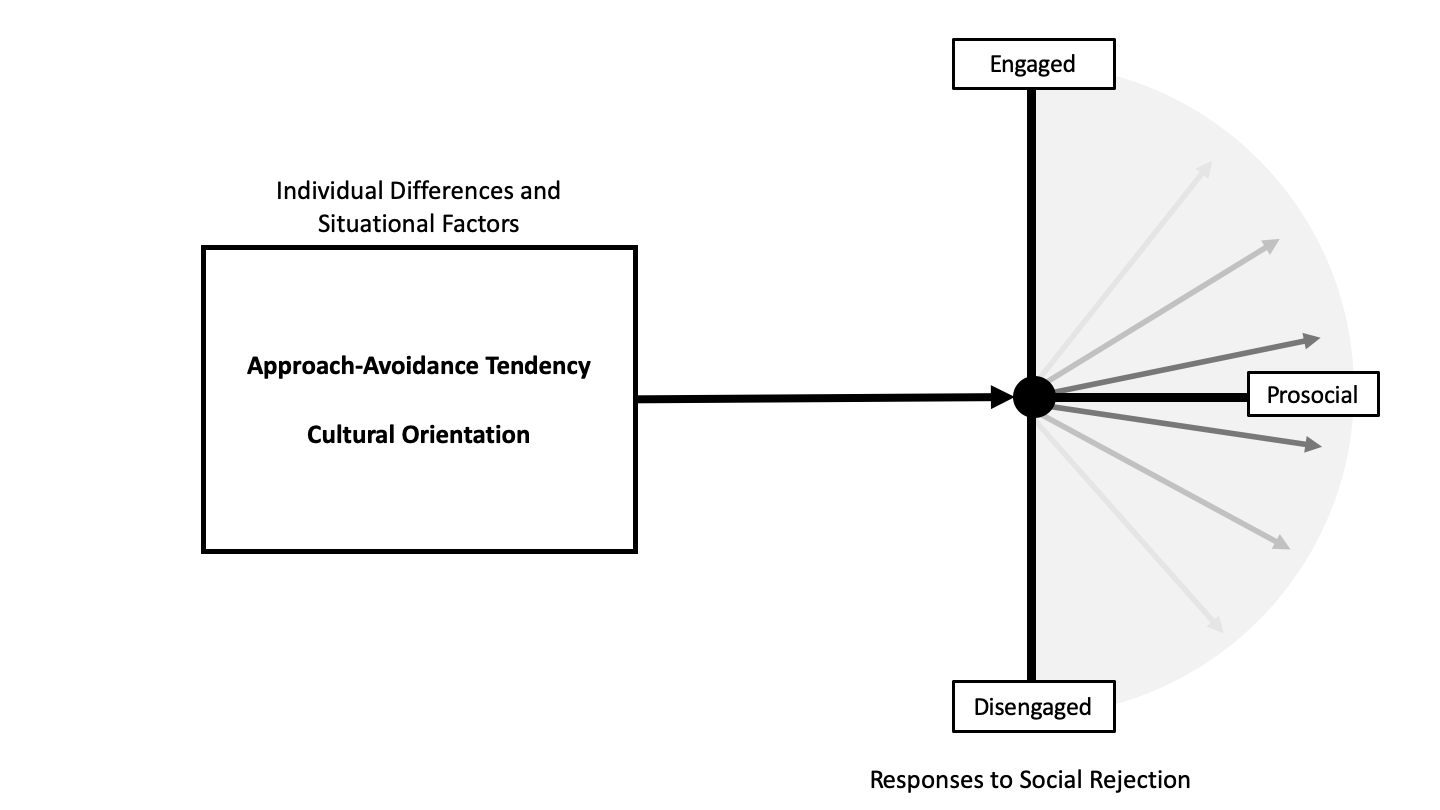
\includegraphics[width=1\linewidth]{images/bidr-prosocial} \caption{Representative individual differences and situational factors predicting prosocial engaged and disengaged responses. Only the prosocial dimension is depicted in this diagram for illustrative purposes. Approach-oriented tendencies and individualistic cultural backgrounds predict engaged prosocial responses. On the other hand, avoidance-oriented tendencies and collectivistic cultural backgrounds predict disengaged prosocial responses.}\label{fig:bidr-prosocial}
\end{figure}

\textbf{Approach-Avoidance Tendency.} People differ in their tendency to
approach or avoid a social outcome. In general, people with
approach-oriented tendencies actively pursue desirable outcomes, whereas
people with avoidance-oriented tendencies avoid undesirable outcomes
(\citeproc{ref-elliotApproachAvoidanceMotivation2006}{Elliot et al., 2006}). In the context of rejection,
the desired outcome is re-establishing belonging, and the undesired
outcome is experiencing further rejection. Ultimately, people must
balance these two goals to maintain meaningful interpersonal
relationships (e.g., \citeproc{ref-murrayOptimizingAssuranceRisk2006}{Murray et al., 2006}). Prior to the
bi-dimensional rejection taxonomy, researchers would predict that
avoidance-oriented people would not display prosocial responses
following rejection, because the types of prosocial responses typically
studied have risks of further rejection (e.g., actively seeking
acceptance from another person). With the taxonomy, we can see that this
hypothesis may not be accurate. Theoretically, people with higher
avoidance tendencies would display prosocial responses, but they would
do so in disengaged ways (e.g., relying on social surrogates) because
this response style matches their general tendency to use hands-off,
avoidance-oriented strategies.

\textbf{Cultural Orientation.} Cultural contexts influence how people rely on
social support, a form of prosocial behavior motivated by a need for
affiliation (\citeproc{ref-choenaromRoleSenseBelonging2005}{Choenarom et al., 2005}; \citeproc{ref-hagertyEffectsSenseBelonging1999}{Hagerty \& Williams, 1999 Jul-Aug}; \citeproc{ref-kimCultureSocialSupport2008}{Kim et al., 2008}).
Compared with people with individualistic backgrounds (e.g., European
Americans), those with collectivistic backgrounds (e.g., Asian
Americans) sought more \emph{implicit} forms of social support---emotional
comfort obtained through the existing social network without directly
discussing one's problems (\citeproc{ref-kimCultureSocialSupport2008}{Kim et al., 2008}). Implicit
support seeking is disengaged because it is a passive behavior that
allows a person to avoid potential rejection and thus future threats to
belonging. On the other hand, explicit support seeking is engaged
because it involves direct communication of the need for support to
close others. Taken together, people with collectivistic backgrounds may
use more disengaged rather than engaged prosocial responses to
rejection, and people with individualistic backgrounds may use more
engaged rather than disengaged prosocial responses to rejection (Figure
\ref{fig:bidr-prosocial}).

These cultural predictions further highlight the risk of neglecting the
engaged-disengaged \emph{y}-axis, and how doing so could lead to incorrect
conclusions. If a researcher measures only engaged prosocial responses
(i.e., explicit support seeking), they would reach the erroneous
conclusion that people from a collectivistic background do not engage in
prosocial behavior following rejection. However, they theoretically
behave prosocially following rejection, but they do so in disengaged
ways (e.g., implicit support seeking). Considering both dimensions of
the bi-dimensional rejection taxonomy will prevent such faulty
conclusions.

\section{Using the Bi-Dimensional Rejection Taxonomy to Inspire New and More Accurate Hypotheses}\label{using-the-bi-dimensional-rejection-taxonomy-to-inspire-new-and-more-accurate-hypotheses}

As we highlight throughout the paper, the bi-dimensional rejection
taxonomy is an important advancement to the rejection literature because
it helps researchers generate more nuanced and accurate hypotheses and
prevents inaccurate conclusions. The taxonomy draws on available
theories to make predictions about which individual and situational
characteristics will predict when people will respond in one way or
another. In doing so, the taxonomy allows researchers to generate
innovative hypothesis incorporating all possible response options. In
this section, we discuss how the bi-dimensional rejection taxonomy
inspires new directions for future research. In contrast to the previous
sections that demonstrated how existing evidence could be viewed through
the lens of the taxonomy, this section purposefully highlights more
speculative and innovative avenues for new research that have yet to be
tested. Thus, the reader should take these future directions with a
grain of salt; they are meant to inspire new and exciting ways to apply
the taxonomy.

\subsection{Spontaneous Reactions to Rejection}\label{spontaneous-reactions-to-rejection}

Past rejection studies relied on laboratory experiments where behavioral
and self-reported response options were constrained. For example, in the
hot-sauce paradigm, participants had no choice but to allocate some
amount of hot sauce to a stranger without an option to respond
differently (Lieberman, Solomon, Greenberg, \& McGregor, 1999). Questions
remain as to how rejected participants respond in real-life settings
where other response options are readily available (e.g., rejected
people can watch their favorite TV show, approach a friend, lash out
against the perpetrator, or withdraw from others). In addition, people
experiencing rejection may use multiple responses simultaneously (e.g.,
watching favorite TV shows and talking to friends after getting dumped).
The existing literature has not investigated which responses people
commonly use following rejection in the real world---an important next
step to advance the literature. One concrete recommendation is to have
at least four types of response options in rejection studies. For
example, daily diary or experience sampling studies could assess whether
rejection occurred that day, and if so, could ask how the participant
responded, ensuring that response options from each quadrant are
included.

Without the bi-dimensional rejection taxonomy, researchers interested in
prosocial responses may inadvertently fail to measure disengaged
prosocial responses (e.g., watching a favorite TV program) and may
instead solely focus on engaged prosocial responses (e.g., approaching a
friend). Doing so brings with it the danger of concluding that prosocial
responses do not happen in response to everyday rejection whereas, in
reality, they may be happening, but in disengaged rather than engaged
manners. Armed with the knowledge of the bi-dimensional rejection
taxonomy, researchers can now avoid this pitfall and include response
options that cover both dimensions.

An unexplored possibility is that people typically react to everyday
rejection in disengaged ways (e.g., social surrogacy and social
withdrawal). Past research has found that interpersonal rejection is
prevalent in everyday life, ranging from subtle ignorance in social
situations (e.g., no eye contact and being looked-through) to more
obvious ones {[}e.g., being ignored in conversations, emails, and online
messaging; Nezlek et al. (\citeproc{ref-nezlekOstracismEverydayLife2012}{2012}){]}. People need to regularly
cope with these rejection experiences to maintain their belonging. As
mentioned earlier, repeated experiences of rejection may promote
disengaged responses, particularly in the antisocial domain. We
speculate a similar pattern for the prosocial domain---people may use
disengaged prosocial responses, rather than engaged prosocial responses
for repeated everyday rejection. People can replenish belonging more
safely through disengaged prosocial responses because they function to
avoid future need threat (i.e., further rejection). The popularity of
TV, books, and social media may reflect people's preference in
satisfying belonging from these disengaged prosocial activities, a
provocative question for future research.

\subsection{Neurophysiological Markers}\label{neurophysiological-markers}

Neurophysiological correlates can provide mechanistic answers about why
rejection leads to responses that fall within the bi-dimensional
rejection taxonomy. Cortisol and testosterone are potentially relevant
hormonal markers that can predict rejection responses. The combination
of high testosterone and low cortisol levels jointly predict
dominance-seeking behaviors, often associated with engaged antisocial
behaviors (e.g., physical fights and violence;
(\citeproc{ref-mehtaTestosteroneCortisolJointly2010}{Mehta \& Josephs, 2010}; \citeproc{ref-platjeTestosteroneCortisolRelation2015}{Platje et al., 2015}; \citeproc{ref-romero-martinezTestosteroneCortisolRatio2013}{Romero-MartÃÂnez et al., 2013}). When cortisol levels are
high, dominance responses are inhibited (and submission responses are
facilitated), regardless of testosterone levels. Thus, one unexamined
hypothesis is that high testosterone and low cortisol levels may
facilitate engaged antisocial responses to rejection. On the other hand,
high cortisol levels may inhibit engaged antisocial responses and may
instead facilitate disengaged antisocial responses (e.g., social
withdrawal and self-neglect).

Considering the interaction between cortisol and testosterone highlights
the importance of the bi-dimensional rejection taxonomy. If researchers
study cortisol and testosterone in the absence of the taxonomy and
measure only engaged antisocial responses, they may conclude that
cortisol levels do not affect antisocial responses at all. In light of
the current taxonomy, this conclusion may be unwarranted---since high
cortisol levels should theoretically facilitate disengaged antisocial
responses.

\subsection{Applying the Bi-Dimensional Rejection Taxonomy to Other Threats to Belonging}\label{applying-the-bi-dimensional-rejection-taxonomy-to-other-threats-to-belonging}

The bi-dimensional rejection taxonomy offers a blueprint for future
researchers who study responses to social stressors that threaten
belonging. Currently, the bi-dimensional rejection taxonomy is focused
on the responses to interpersonal rejection (e.g., feeling uncared for
or unloved). But, other social stressors can also threaten belonging,
such as separation distress {[}e.g., feelings of missing someone;
Diamond et al. (\citeproc{ref-diamondEveryTimeYou2008}{2008}){]}, death of a close other
(\citeproc{ref-stroebeRoleLonelinessSocial1996}{Stroebe et al., 1996}), and
discrimination(\citeproc{ref-richmanReactionsDiscriminationStigmatization2009}{Richman \& Leary, 2009}). One
interesting application of the bi-dimensional rejection taxonomy would
be to examine whether responses to these belonging threats also range
along the antisocial--prosocial and engaged--disengaged dimensions.
Doing so will facilitate a richer understanding of how humans respond to
belonging threats.

\section{Conclusion}\label{conclusion}

Existing theories of interpersonal rejection have exclusively focused on
the \emph{x}-axis, aiming to understand antisocial and prosocial responses to
interpersonal rejection. Accumulating evidence suggests a gap in this
approach: variability in social responses to rejection cannot solely be
explained by the antisocial--prosocial dimension alone. To fill this
gap, we propose the bi-dimensional rejection taxonomy, consisting of the
antisocial--prosocial \emph{x}-axis and engaged--disengaged \emph{y}-axis, a novel
contribution to the literature. This engaged--disengaged dimension
explains variation among prosocial and antisocial responses previously
unaccounted for, helps researchers to generate more nuanced and accurate
hypotheses about how people respond to rejection, and sheds light on the
types of responses that have been understudied in the literature. Thus,
the bi-dimensional rejection taxonomy is an important step forward for
the rejection literature. Overlooking the engaged--disengaged dimension
could result in omnibus hypotheses that lack specificity, leading to
erroneous and inaccurate conclusions. The bi-dimensional rejection
taxonomy helps researchers to see nuances among responses, better
calibrate conclusions, and test novel predictions. With this new map, we
can move the literature to new frontiers.

\chapter{Current Dissertation}\label{current-dissertation}

Does Solo Gameplay Replenish Belonging After Social Rejection?

The bi-dimensional rejection taxonomy identifies disengaged-prosocial
responses as an emerging category of behavioral responses to social
rejection (\citeproc{ref-sunamiBIDimensionalRejectionTaxonomy2020}{Sunami et al., 2020}). Since this category is novel, identifying new
disengaged-prosocial responses benefits the literature. One potential
unexamined disengaged-prosocial response is solo gameplay: gameplays
without any other human players. Solo gameplay is disengaged and
prosocial since players play alone by themselves and satisfy belonging
in an indirect, passive, hands-off manner from the non-human entities in
a game (\citeproc{ref-sunamiBIDimensionalRejectionTaxonomy2020}{Sunami et al., 2020}). Theoretically, solo gameplay should replenish
belonging via social surrogates (\citeproc{ref-gabrielSocialSurrogatesRejection2017}{Gabriel \& Valenti, 2017}). However, no quantitative
studies have tested this possibility. In my dissertation, I examined
whether solo gameplay can replenish belonging after social rejection.

In this chapter, I discuss a theoretical foundation for the hypothesis
that solo gameplay can replenish belonging following social rejection. I
first discuss the social surrogacy hypothesis (\citeproc{ref-gabrielSocialSurrogatesRejection2017}{Gabriel \& Valenti, 2017}). This
hypothesis suggests that people can fulfill belonging from \emph{social
surrogates}: targets with only psychological bonds without actual social
interactions. I focus on two types of social surrogates relevant to
single-player games, namely parasocial relationships and social worlds.
For each type of social surrogate, I draw from video game research to
discuss how video games can provide a social surrogate. Finally, I
introduce the research question and the hypotheses of my dissertation.

\section{The Social Surrogacy Hypothesis: Purely Psychological Bonds that Fulfill Belonging}\label{the-social-surrogacy-hypothesis-purely-psychological-bonds-that-fulfill-belonging}

People can satisfy their fundamental need to belong via
engaged-prosocial behaviors such as affectionate exchanges with one's
romantic partner, family members, and friends (\citeproc{ref-baumeisterNeedBelongDesire1995}{Baumeister \& Leary, 1995}).
However, an interaction with a real person is not the only way to
satisfy belonging---people can replenish belonging via
disengaged-prosocial behaviors such as feeling connected with fictional
characters in books (\citeproc{ref-gabrielSocialSurrogatesRejection2017}{Gabriel \& Valenti, 2017}). Just as people have used substitutes
to satisfy other fundamental needs (e.g., coca leaves for hunger,
caffeine for sleep), people can use \emph{social surrogates} to substitute
real social connections. Social surrogates are human or non-human
targets to which people form symbolic bonds without actual social
interactions (\citeproc{ref-derrickSocialSurrogacyHow2009}{Derrick et al., 2009}; \citeproc{ref-gabrielSocialSurrogatesRejection2017}{Gabriel \& Valenti, 2017}). The social surrogacy
hypothesis suggests three types of social surrogates: parasocial
relationships (e.g., feeling connected to a favorite TV character),
social worlds (e.g., feeling like a member of a collective in a fantasy
novel), and reminders of others (e.g., feeling connected by looking at
photos of loved ones). I focus on parasocial relationships and social
worlds since video games can provide an opportunity for both, as
discussed later. I do not include reminders of others since they are
based on real social relationships by definition, and are thus absent in
solo gameplay.

\section{Parasocial relationships}\label{parasocial-relationships}

\subsection{Definition}\label{definition}

Parasocial relationships refer to one-way emotional bonds and feelings
of intimacy without an actual social interaction (\citeproc{ref-gabrielSocialSurrogatesRejection2017}{Gabriel \& Valenti, 2017}; \citeproc{ref-knowlesBelongingRegulationUse2013}{Knowles, 2013}). People sometimes feel like they are friends with
celebrities (e.g., Cardi B) or fictional characters (e.g., Derrick
Morgan from Criminal Minds); they feel like they ``know'' the person and
are psychologically connected to them. People even become romantically
attracted to fictional characters (\citeproc{ref-liebers2017}{Liebers \& Schramm, 2017}). Past research showed
that people form parasocial relationships with various targets:
fictional characters in books and TV programs, celebrities, and Formula
1 drivers (\citeproc{ref-derrick2008}{Derrick et al., 2008}; \citeproc{ref-hartmann2008}{Hartmann et al., 2008}; \citeproc{ref-horton1956}{Horton \& Wohl, 1956}; \citeproc{ref-rubin1985}{A. M. Rubin et al., 1985}; \citeproc{ref-rubin1987}{R. B. Rubin \& McHugh, 1987}; \citeproc{ref-schmid2011}{Schmid \& Klimmt, 2011}).

Parasocial relationships are similar to real social relationships in
some ways. First, people tend to form both real and parasocial
relationships with similar others. In real social relationships, people
form stronger bonds with others who appear similar to themselves than
those who do not (\citeproc{ref-montoya2008}{Montoya et al., 2008}). Similarly, people form stronger
parasocial relationships with television performers and book characters
when they see similarities in attitudes, beliefs, and values than when
they do not (\citeproc{ref-liebers2017}{Liebers \& Schramm, 2017}; \citeproc{ref-turner1993}{Turner, 1993}). Second, breaking up with or
losing a parasocial relationship partner can be emotionally hurtful as
losing a real relationship (\citeproc{ref-cohen2003}{J. Cohen, 2003}; \citeproc{ref-eyal2006}{Eyal \& Cohen, 2006}; \citeproc{ref-lather2011}{Lather \& Moyer-Guse, 2011}). In real
social relationships, people experience distress for breakups and grief
for losing a loved one (\citeproc{ref-lobb2010}{Lobb et al., 2010}; \citeproc{ref-lundorff2017}{Lundorff et al., 2017}; \citeproc{ref-sbarra2006}{Sbarra \& Ferrer, 2006}).
Likewise, when the American TV sitcom \emph{Friends} ended, viewers with
stronger parasocial relationships with Friends characters reported
becoming lonelier and missing their favorite character more than those
with weaker parasocial relationships (\citeproc{ref-eyal2006}{Eyal \& Cohen, 2006}). People with stronger
parasocial relationships with the celebrity Robin Williams reported more
grief over Williams' death than those with weaker parasocial
relationships (\citeproc{ref-cohen2016}{E. L. Cohen \& Hoffner, 2016}). People also experience distress when they
are temporarily separated from a parasocial target, similar to missing a
loved one in real social relationships (\citeproc{ref-le2008}{Le et al., 2008}, \citeproc{ref-le2011}{2011}). For instance,
during the writer's strike in 2007--2008 when TV companies stopped
airing new episodes, TV viewers lost opportunities to parasocially
interact with their favorite TV characters. During this time, people
with stronger parasocial relationships with TV characters were more
distressed and lonelier than those with weaker parasocial relationships
(\citeproc{ref-lather2011}{Lather \& Moyer-Guse, 2011}).

Despite the similarities, parasocial relationships are different from
real social relationships in at least two ways. First, parasocial
relationships are one-way and nonreciprocal, whereas real social
relationships are two-way and reciprocal. In contrast to a real
relationship where both partners can communicate with each other, in a
parasocial relationship the media consumer is the only one who forms a
psychological bond to the media figure, without an opportunity to
influence the media figure and receive a response (\citeproc{ref-cohen2014}{J. Cohen, 2014}; \citeproc{ref-horton1956}{Horton \& Wohl, 1956}). Second, parasocial relationships tend to be weaker in
strength than real social relationships. People reported that they were
less satisfied, less invested, and less committed to parasocial
relationships with their favorite media figure than to an actual
relationship with their close friends and family members (\citeproc{ref-eyal2012}{Eyal \& Dailey, 2012}).
Overall, while parasocial relationships can benefit people's belonging,
they may not substitute actual close relationships.

\subsection{Parasocial Relationships in Video Games}\label{parasocial-relationships-in-video-games}

In the early role-playing and adventure video games of the 1970s, most
non-player characters were enemies (e.g., trolls, dragons, etc.), and
thus players had few opportunities to form emotional bonds with video
game characters. Later in the 1980s, video games began to present
relatable non-player characters. For example, \emph{King's Quest}
(\citeproc{ref-on-line1984a}{On-Line, 1984}) included dialogues with the king, the elf, and the
woodcutter, where players could get to know about these non-player
characters. In the 1980-90s, Japanese game developers created the
\emph{dating games} genre where players could form strong romantic
relationships with other characters. For example, in \emph{Tokimeki Memorial}
(``Heartbeat Memorial''), the player takes the role of a male high school
student who dates female non-player characters to seek \emph{eternal love}
(\citeproc{ref-corporation1994a}{Corporation, 1994}; \citeproc{ref-pollack1996}{Pollack, 1996}). A media report even suggested that
some players became so emotionally attached to their favorite characters
that they started to send love letters and birthday cards to the
characters (\citeproc{ref-pollack1996}{Pollack, 1996}).

Modern adventure and role-playing games also present relatable
non-player characters with whom players can form parasocial
relationships (\citeproc{ref-tyack2017}{Tyack \& Wyeth, 2017}). For example, players of \emph{Mass Effect 2}
(\citeproc{ref-bioware2010}{BioWare, 2010}) reported forming intense emotional bonds with characters
(Garrus or Tali) similar to romantic relationships (\citeproc{ref-burgess2020a}{Burgess \& Jones, 2020}).
Among women who played dating games, those with more playtime formed a
stronger parasocial relationship with a virtual romantic partner than
those with less playtime (\citeproc{ref-song2016}{Song \& Fox, 2016}). Thus, people can form parasocial
relationships with non-player characters in video games and possibly
replenish belonging. However, the bulk of research has been anecdotal,
qualitative, and theoretical, and no studies have examined whether
people can rely on parasocial relationships to cope with social
rejection. In the current dissertation, I provide quantitative evidence
on whether parasocial relationships in video games can replenish
belonging after social rejection. Based on the social surrogacy
hypothesis, I hypothesized that rejected people who play a single-player
video game with higher parasocial relationship content would report
higher belonging than those who play a game with lower parasocial
relationship content.

\section{Social Worlds}\label{social-worlds}

\subsection{Definition}\label{definition-1}

Social worlds are stories, narratives, and collectives to which people
assimilate (\citeproc{ref-gabrielSocialSurrogatesRejection2017}{Gabriel \& Valenti, 2017}). When consuming a narrative (e.g., reading or
watching), people immerse themselves in the story and transport
themselves into the social world described in the narrative
(\citeproc{ref-gabrielBecomingVampireBeing2011}{Gabriel \& Young, 2011}). As a result, people can assimilate themselves as a
member of the collective in the story---a process called narrative
collective-assimilation (\citeproc{ref-gabrielSocialSurrogatesRejection2017}{Gabriel \& Valenti, 2017}; \citeproc{ref-gerrig1993}{Gerrig, 1993}; \citeproc{ref-green2004}{Green, 2004}; \citeproc{ref-mar2008}{Mar \& Oatley, 2008}). For example, participants who read a passage from Harry
Potter reported that they felt like a member of the magical world of
Harry Potter---people felt like being British, able to move an object,
and able to make themselves disappear magically (\citeproc{ref-gabrielBecomingVampireBeing2011}{Gabriel \& Young, 2011}). On the
other hand, participants who read a passage from Twilight identified
themselves as a vampire---people felt like having sharper teeth and
being able to jump higher and stay awake longer. Thus, people can
immerse and assimilate into a collective in a social world, and
theoretically, can feel belonging. Indeed, people with a higher need to
belong are more likely to immerse themselves in stories than those with
a lower need to belong (\citeproc{ref-greenwood2009}{Greenwood \& Long, 2009}). Socially rejected people who
recalled their favorite TV program (providing social worlds) reported
higher belonging than those who recalled a non-favorite TV program
(\citeproc{ref-derrickSocialSurrogacyHow2009}{Derrick et al., 2009}).

Researchers have used different terms to describe the process by which
people immerse in a social world, such as \emph{transportation}, \emph{flow},
\emph{cognitive absorption}, \emph{and} \emph{presence} (\citeproc{ref-agarwal2000}{Agarwal \& Karahanna, 2000}; \citeproc{ref-csikszentmihalyi2008}{Csikszentmihalyi, 2008}; \citeproc{ref-green2004}{Green, 2004}; \citeproc{ref-green2000}{Green \& Brock, 2000}; \citeproc{ref-patrick2000}{Patrick et al., 2000}; \citeproc{ref-pine1999}{Pine \& Gilmore, 1999}).
In my dissertation, I use \emph{immersion} as an overarching term to describe
the process whereby players immerse themselves and assimilate to the
collective in a video game.

\subsection{Social Worlds in Video Games}\label{social-worlds-in-video-games}

Like books, TV shows, and movies, many modern video games provide social
worlds for players to immerse themselves in, assimilate with, and feel
connected to the collectives in the stories
(\citeproc{ref-bormannImmersedVirtualWorlds2015}{Bormann \& Greitemeyer, 2015}; \citeproc{ref-domschStoryplayingAgencyNarrative2013}{Domsch, 2013}; \citeproc{ref-greenTransportationTheory2017}{Green \& Sestir, 2017}).
For example, players can be a soldier of System Alliance in \emph{Mass
Effect}, a citizen of Tamriel in \emph{Elder Scrolls}, a gang in Liberty City
in \emph{Grand Theft Auto}, and a boy from Pallet Town (\emph{Masara} Town) in
\emph{Pokemon}. Video games often provide audio and visual cues that
facilitate the player's immersion into the social world. Players can
hear the noises of busy streets, sounds of trees swinging by wind, or
chatters of other characters. Players see roads, vehicles, houses, and
buildings that represent a collective in the video game. They learn
about the story and feel like being a character in the world as they
experience those visual and audio cues.

Can people replenish belonging by immersing themselves in a social world in a
single-player video game? In one study, half of the participants were
told to ignore the story whereas the other half read a backstory of the
game (\citeproc{ref-bormannImmersedVirtualWorlds2015}{Bormann \& Greitemeyer, 2015}). Then, participants played
\emph{Gone Home}, a single-player adventure game with a rich narrative.
Participants who read the backstory experienced higher immersion and
higher belonging than those who ignored the story
(\citeproc{ref-bormannImmersedVirtualWorlds2015}{Bormann \& Greitemeyer, 2015}). Based on the social surrogacy
hypothesis, I hypothesized that rejected people who play a single-player
video game with higher social worlds content would report higher
belonging than those who play a game with lower social worlds content.

\section{Focusing on Solo Play}\label{focusing-on-solo-play}

Both single-player and multiplayer games can potentially provide
parasocial relationships and social worlds. For example, players of
massively online multiplayer role-playing games (MMORPG) can experience
social surrogates by feeling a personal connection to Arthas Menethil in
the World of Warcraft or feeling like a member of the race Lalafell in
\emph{Final Fantasy IV}. However, players can also interact with other real
players in multiplayer and thus replenish their belonging via real
social interactions, without social surrogacy (\citeproc{ref-kowert2015}{Kowert \& Oldmeadow, 2015}; \citeproc{ref-vella2015}{Vella et al., 2015}).
Since the goal of my dissertation is to examine playing a video game as
a disengaged-prosocial response without real social interactions, I
exclusively focused on solo gameplay.

\section{Focusing on Outcome, not Mechanism}\label{focusing-on-outcome-not-mechanism}

In my dissertation, I focused on whether playing a single-player video
game with social surrogates can increase belonging after social
rejection. Since this is the first study to examine this novel
possibility, I did not focus on examining the mechanisms in which
social surrogates can increase belonging, an important area for future
research. Multiple mechanisms are possible for social surrogates to
replenish belonging following social rejection. Social surrogates can
directly replenish belonging as the social surrogacy hypothesis
suggests. Or, social surrogates can replenish belonging via other
intermediary psychological processes. For example, playing a video game
can make the player feel happy, competent, autonomous, self-confident,
or even distracted following social rejection---all of which could
increase belonging (\citeproc{ref-hales2016}{Hales et al., 2016}; \citeproc{ref-learySelfesteemInterpersonalMonitor1995}{Leary et al., 1995}; \citeproc{ref-wesselmann2013}{Wesselmann et al., 2013}; \citeproc{ref-williamsOstracismTemporalNeedthreat2009}{Williams, 2009}). While these are all interesting possibilities, the goal
of my dissertation is to test whether social surrogates are effective to
replenish belonging in single-player games. Without knowing whether they
can replenish belonging, any efforts to examine why they do so would be
inefficient. If I find that the social surrogates replenish belonging in
single-player games, then we can start investigating possible
mechanisms. With that being said, I included a few ancillary measures
that assessed some of these possibilities (e.g., enjoyment, valence, and
dominance), but this was not the main goal of this dissertation.

\section{Do Parasocial Relationships and Social Worlds Influence Each Other?}\label{do-parasocial-relationships-and-social-worlds-influence-each-other}

The social surrogacy hypothesis suggests that parasocial relationships
and social worlds are distinct processes, relatively independent from
each other (\citeproc{ref-gabrielSocialSurrogatesRejection2017}{Gabriel \& Valenti, 2017}). Theoretical discussions in the communications
literature support this independence. People can immerse themselves in a
story without forming a parasocial relationship; conversely, people can
form a parasocial relationship without immersing themselves in a story
(\citeproc{ref-greenTransportationTheory2017}{Green \& Sestir, 2017}). For example, readers of Harry Potter
can feel like a student at Hogwarts, without feeling close to Harry,
Hermionie, or Ron. Similarly, readers can develop parasocial
relationships with the characters, without feeling like a member of a
collective in the social world.

Although parasocial relationships and social worlds are independent,
they could positively influence each other
(\citeproc{ref-brownExaminingFourProcesses2015}{Brown, 2015}; \citeproc{ref-vordererEnjoymentHeartMedia2004}{Vorderer et al., 2004}).
Highly immersed players may form stronger parasocial relationships with
the characters than non-immersed players. Likewise, players with
stronger parasocial relationships with the characters may immerse more
in the story than those with weaker parasocial relationships. Existing
research supports this relationship between parasocial relationships and
social worlds. A theory of media entertainment suggests that people
enjoy media the most when they experience parasocial relationships and
immersion at the same time (\citeproc{ref-vordererEnjoymentHeartMedia2004}{Vorderer et al., 2004}). In a
quantitative study, people who were immersed more in a story reported
stronger parasocial relationships than those who did not
(\citeproc{ref-slaterExtendingConceptualizationMeasurement2018}{Slater et al., 2018}). After watching a
novel TV episode, people who formed stronger parasocial relationships
with the characters reported feeling more immersed in the story than
those who formed weaker parasocial relationships
(\citeproc{ref-ericksonExperimentalExaminationBinge2019}{Erickson et al., 2019}). Taken together, I
hypothesize that the effects of parasocial relationships and social
worlds can add up to benefit belonging (Hypothesis 4). However, the
social surrogacy hypothesis makes no clear prediction about whether the
relationship between parasocial relationships and social worlds would be
additive or synergistic. Thus, I treated this hypothesis as ancillary.

\section{Current Dissertation}\label{current-dissertation-1}

In this dissertation, I asked whether solo gameplay can replenish
belonging after social rejection---whether socially rejected people
could restore their sense of belonging by playing a video game in
single-player mode. I start my dissertation by validating a new measure
of state belonging, the Heart Manikin (Study 1), because a flexible
state measure of belonging does not currently exist. I used this measure
as a primary outcome throughout my dissertation.

In Study 2, I asked rejected participants to write about a time they
played a video game with social surrogates vs.~a video game without
social surrogates. I hypothesized that rejected people who write about
their regularly played video game with social surrogates would report
higher belonging than those who write about a regularly played game
without social surrogates (Hypothesis 1).

Contrasting social surrogate video games and non-social surrogate video
games in Study 2 provides preliminary evidence of whether rejected
people can replenish their belonging by social surrogates in
single-player games. However, whether parasocial relationships, social
worlds, or a combination of the two influenced belonging remains
unknown. To resolve these issues, I asked participants to play a novel,
custom single-player game with higher vs.~lower parasocial relationships
and social world contents in Study 3. I hypothesized that rejected
people who play a video game with higher parasocial relationship content
would report higher belonging than those who play a video game with
lower parasocial relationship content (Hypothesis 2). Similarly,
rejected people who play a video game with higher social world content
would report higher belonging than those who play a video game with
lower social world content (Hypothesis 3). As an ancillary hypothesis, I
expected an additive effect of parasocial relationships and social
worlds: rejected people who play a video game with higher parasocial
content and higher social world contents would report the highest
belonging among all groups (Hypothesis 4).

\section{Open Science Statement}\label{open-science-statement}

To reduce biases from post-hoc, data-dependent inferences, and
researchers' degrees of freedom, I pre-registered my hypotheses and
research plans on the Open Science Framework. To maximize the
transparency and reproducibility of the results, I uploaded materials,
analysis scripts, and de-identified data to the Open Science Framework
(\url{https://osf.io/hydxk/}) and GitHub
(\url{https://github.com/nsunami/dissertation}) so that other researchers
can reproduce and verify the results.

\chapter{Study 1: Validating The Heart Manikin and The Rejection Manipulation}\label{study-1-validating-the-heart-manikin-and-the-rejection-manipulation}

The critical outcome measure for my dissertation is a state measure of
belonging---that captures how much participants feel accepted,
connected, loved, and cared for at a given moment. My dissertation
required a new scale since existing scales focus on measuring belonging
in a group context or belonging as an individual difference. For
example, the need-threat scale (\citeproc{ref-williamsOstracismTemporalNeedthreat2009}{Williams, 2009}), measures how one felt
rejected by a group in Cyberball (e.g., ``I felt the other players
interacted with me a lot'', ``I felt I belonged to the group''). The UCLA
loneliness scale (\citeproc{ref-russell1996}{Russell, 1996}) measures threatened belonging at the
individual difference level, not at the state level (e.g., ``How often do
you feel that you lack companionship?''). In this study, I developed a new scale
that is unconstrained in a group context and measures a state belonging.

In Studies 2 and 3, I planned to have all participants complete a social
rejection induction essay from previous studies (\citeproc{ref-sunamiDoesProspectFulfilling2019}{Sunami et al., 2019}; \citeproc{ref-twengeIsnItFun2003}{Twenge \& Campbell, 2003}), without a control or acceptance condition to reduce the
number of participants and costs. Since various forms of this
manipulation have been successfully used in many labs to induce
rejection, I was initially confident that this manipulation would be
effective. To further ensure that this particular social rejection
induction was effective before running my primary studies, I examined
the effectiveness of the rejection manipulations in Studies 1c and 1e.

\section{The Heart Manikin}\label{the-heart-manikin}

To provide a suitable measure for my dissertation, I proposed the Heart
Self-Assessment Manikin scale, a new single-item measure of belonging
(Figure \ref{fig:heart-manikin}). The Heart Self-Assessment Manikin is
an adapted version of the Self-Assessment Manikin (Figure
\ref{fig:original-manikins}) that measures emotional valence, arousal,
and dominance in a given moment (\citeproc{ref-bradleyMeasuringEmotionSelfAssessment1994}{Bradley \& Lang, 1994}; \citeproc{ref-langBehavioralTreatmentBiobehavioral1980}{P. J. Lang, 1980}). The original
Self-Assessment Manikin showed good convergent validity with existing
verbal measures (\citeproc{ref-bradleyMeasuringEmotionSelfAssessment1994}{Bradley \& Lang, 1994}). In the original Self-Assessment
Manikin, participants see pictorial figures and choose a number
corresponding to a figure that best describes their current feelings (valence, arousal, dominance).
Likewise, the Heart Self-Assessment Manikin asks participants to
indicate the number best reflects their current belonging. Similar to
the original Self-Assessment Manikin, the Heart Self-Assessment Manikin
is easy to administer, quick to complete, and easily understood by
participants relative to a traditional text-based questionnaire.

\begin{figure}
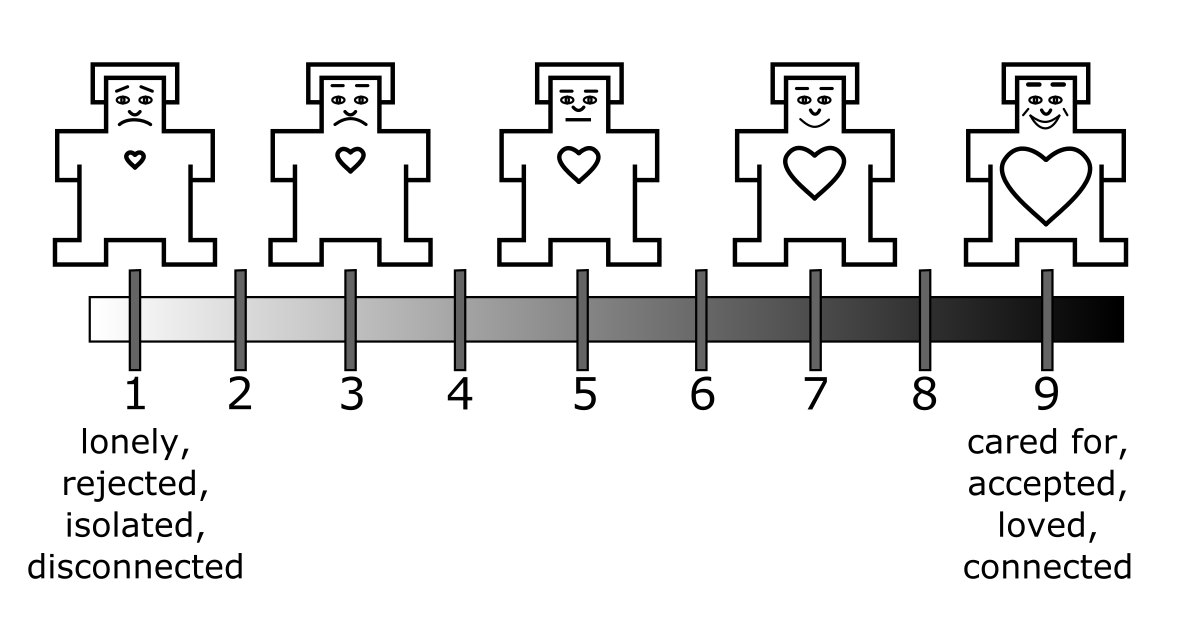
\includegraphics[width=1\linewidth]{images/m-heart} \caption{The Heart Manikin}\label{fig:heart-manikin}
\end{figure}

\emph{Note.} Participants indicate how they feel at the moment on a 9-point
scale. The body and the face of the figure is taken from the valence
subscale of the original Self-Assessment Manikin (\citeproc{ref-langBehavioralTreatmentBiobehavioral1980}{P. J. Lang, 1980}).

\begin{figure}
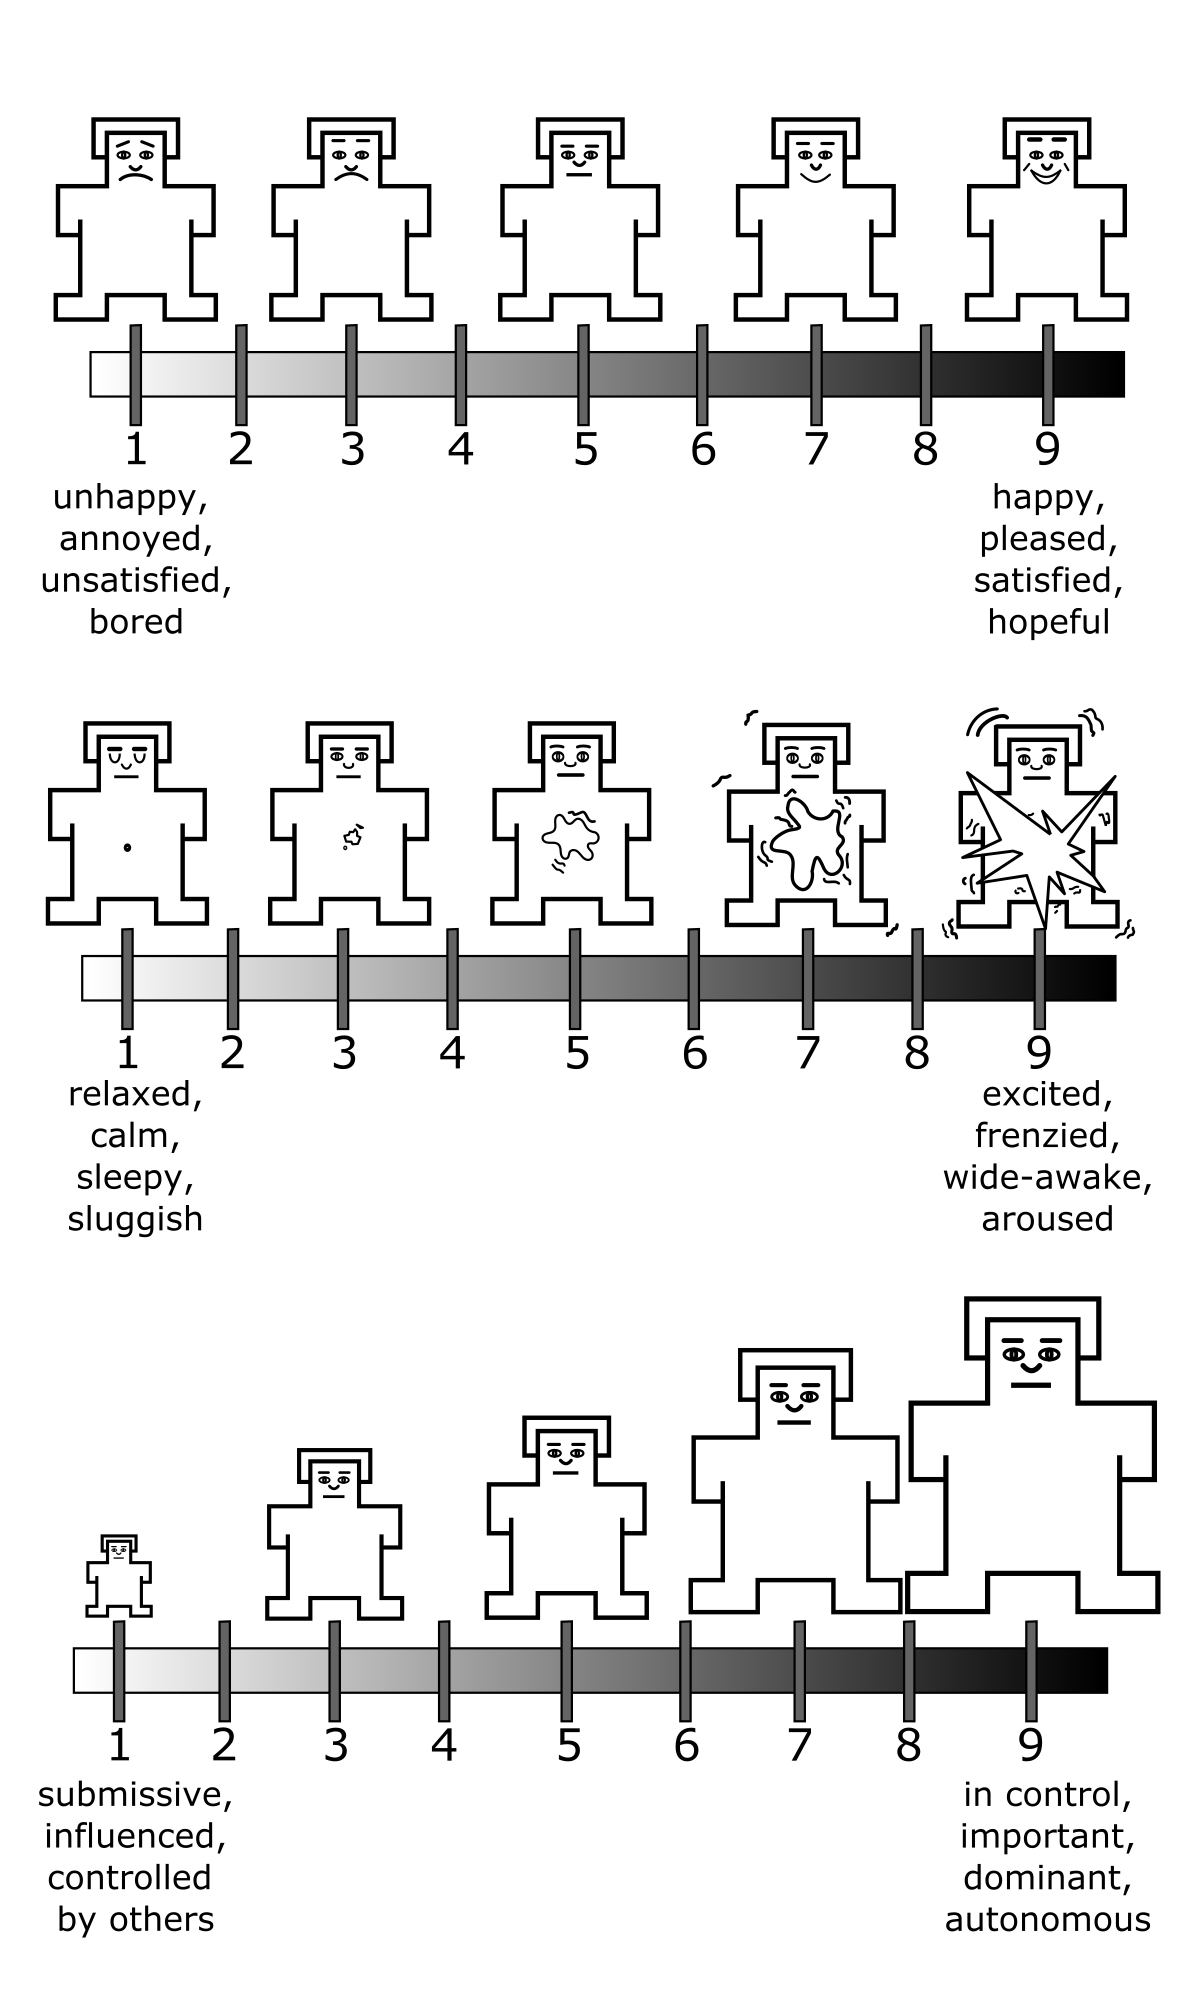
\includegraphics[width=16.42in]{images/m-original-all} \caption{The original Self-Assessment Manikin (Lang, 1980)}\label{fig:original-manikins}
\end{figure}

\emph{Note}. From top to bottom, the items refer to valence, arousal, and
dominance, respectively. Participants indicate how they feel at the
moment on a 9-point scale. The scale has been validated as a state
measure (\citeproc{ref-langBehavioralTreatmentBiobehavioral1980}{P. J. Lang, 1980}). The vector drawings of the valence and arousal
items are adopted from an existing GitHub repository at
\url{https://github.com/hexa-/SAM-vectors} (\citeproc{ref-hexa-2020a}{hexa-, 2020})

\section{Current Study}\label{current-study}

In Study 1, I evaluated construct validity and test-retest reliability
of the Heart Manikin, using five existing datasets (Studies 1a, 1b, 1c,
1d, and 1e). For construct validity, I focused on convergent validity,
discriminant validity, and the scale's sensitivity to a laboratory
manipulation already known to affect belonging (\citeproc{ref-boateng2018}{Boateng et al., 2018}). In
addition, I tested the effectiveness of the rejection manipulation to be
used in the subsequent dissertation studies (Study 1e).

\subsection{Convergent Validity}\label{convergent-validity}

If the Heart Manikin measures belonging, it should correlate with other
measures of belonging. Thus, I expected that the Heart Manikin would
converge measures of belonging {[}Studies 1c, 1d, and 1e; Williams (\citeproc{ref-williamsOstracismTemporalNeedthreat2009}{2009}){]} and social isolation
(Study 1b). I also expected that the heart Manikin scores would also converge
with measures of depression (Study 1a) since lonely people experience
more depressive symptoms than non-lonely people (\citeproc{ref-cacioppoLonelinessSpecificRisk2006}{Cacioppo et al., 2006}; \citeproc{ref-jaremkaLonelinessPredictsPain2013}{Jaremka, Fagundes, Glaser, et al., 2013}; \citeproc{ref-jaremkaPainDepressionFatigue2014}{Jaremka et al., 2014}).

The belonging need is pervasive---people with lower belonging may also
experience lower self-esteem, a lower sense of control, and lower
sense of meaning (\citeproc{ref-hartgerinkOrdinalEffectsOstracism2015}{Hartgerink et al., 2015}; \citeproc{ref-learySelfesteemInterpersonalMonitor1995}{Leary et al., 1995}; \citeproc{ref-williamsOstracismTemporalNeedthreat2009}{Williams, 2009}). Thus, I expected
that the Heart Manikin scores converge with the measures of self-esteem,
control, and a sense of meaning (Studies 1c, 1d, and 1e).

Socially accepted people experience positive emotions; socially rejected people experience negative
emotions (\citeproc{ref-gerberBeingRejectedMetaanalysis2009}{Gerber \& Wheeler, 2009}; \citeproc{ref-richmanReactionsDiscriminationStigmatization2009}{Richman \& Leary, 2009}; \citeproc{ref-williamsOstracismTemporalNeedthreat2009}{Williams, 2009}). The
valence scores of the Self-Assessment Manikin (\citeproc{ref-bradleyMeasuringEmotionSelfAssessment1994}{Bradley \& Lang, 1994}) measures how
positively or negatively a person is feeling at a moment. Thus, I
expected that the Heart Manikin scores would positively correlate with
the valence scores of the original Self-Assessment Manikin (Studies 1a,
1b, 1c, 1d, 1e).

People who expect and fear social rejection tend to report lower belonging
than those who do not since they are prone to act in ways to elicit
social rejection from others, akin to self-fulfilling prophecy (\citeproc{ref-downeySelffulfillingProphecyClose1998}{Downey, Freitas, et al., 1998}). Thus, I
expected that the Heart Manikin scores would negatively correlate with
the measures of sensitivity of social rejection, including rejection
sensitivity (Study 1e), fear of negative evaluation (Study 1e), and
avoidant and anxious attachment styles (Study 1e).

People with a caring and nurturing relationship with their romantic
partner should report higher belonging than those who do not. Thus, I
expected that the Heart Manikin scores would positively correlate with
the degree of support that they receive from their partner, the
relationship quality, and closeness to their partner, and perceived
responsiveness of their partner (Study 1b). Conversely, the heart
manikin scores should negatively correlate with the measures of
conflicts, ostracism, psychological and physical abuse in a romantic
relationship (Studies 1b and 1c).

\subsection{Discriminant validity}\label{discriminant-validity}

If the Heart Manikin scale measures state belonging, its scores should
be discriminant against measures of other unrelated constructs. To
examine discriminant validity, I explored correlations between the Heart
Manikin scores with the following measures: arousal and dominance
subscales of the Self-Assessment Manikin
{[}Studies 1a, 1c, 1d, and 1e; Bradley \& Lang (\citeproc{ref-bradleyMeasuringEmotionSelfAssessment1994}{1994}); P. J. Lang (\citeproc{ref-langBehavioralTreatmentBiobehavioral1980}{1980}){]}, beliefs about
biological differences between Black and White people
{[}Study 1a; Hoffman et al. (\citeproc{ref-hoffmanRacialBiasPain2016}{2016}){]},
interpersonal reactivity
{[}Study 1a; Davis (\citeproc{ref-davisMultidimensionalApproachIndividual1980}{1980}){]}, self-monitoring
tendencies {[}Study 1a; Snyder (\citeproc{ref-snyderSelfmonitoringExpressiveBehavior1974}{1974}){]}, tendency to be
excited by paradoxes {[}Study 1a; Miron-Spektor et al. (\citeproc{ref-miron-spektorMicrofoundationsOrganizationalParadox2018}{2018}){]}, capacity to
acknowledge and integrate competing opinions of others
{[}Study 1a; Zhang et al. (\citeproc{ref-zhangParadoxicalLeaderBehaviors2015}{2015}){]}, membership
to different social groups {[}Study 1a; Haslam et al. (\citeproc{ref-haslamMaintainingGroupMemberships2008}{2008 Oct-Dec}){]},
subjective social
status {[}Studies 1b, 1c, and 1e;
Adler et al. (\citeproc{ref-adlerRelationshipSubjectiveObjective2000}{2000}){]}, perpetration of
abusive and controlling behaviors in a romantic relationship {[}Study 1b;
Graham-Kevan \& Archer (\citeproc{ref-graham-kevanPhysicalAggressionControl2003}{2003}) and Postmus et al. (\citeproc{ref-postmusAbusiveBehaviorInventory2015}{2015}){]},
food cravings (Study 1b), dietary social support (Study 1b), body image (Study 1b), levels of
physical activity {[}Study 1b;
Godin (\citeproc{ref-godinGodinShephardLeisureTimePhysical2011}{2011}){]}, sleep quality
{[}Study 1b; Cella et al. (\citeproc{ref-cellaPROMISAdultHealth2019}{2019}){]}, narcissism {[}Study
1b; Konrath et al. (\citeproc{ref-konrathDevelopmentValidationSingle2014}{2014}){]},
perceived psychological stress {[}Study 1b;
S. Cohen et al. (\citeproc{ref-cohenGlobalMeasurePerceived1983}{1983}){]}, the need for closure
{[}Study 1d; Kruglanski (\citeproc{ref-kruglanskiMotivationsJudgingKnowing1990}{1990}){]}, and adherence to
traditional social values {[}Study 1d; Proulx \& Heine (\citeproc{ref-proulxCaseTransmogrifyingExperimenter2008}{2008}); Rosenblatt et al. (\citeproc{ref-rosenblattEvidenceTerrorManagement1989}{1989}){]}.

\subsection{Scale's Sensitivity to Social Rejection Manipulation}\label{scales-sensitivity-to-social-rejection-manipulation}

If the Heart Manikin measures state belonging, the scores should be
sensitive to social rejection manipulations. Studies 1c, 1d, and 1e
included variants of social rejection manipulations commonly used in
social rejection research. Since previous studies have already demonstrated
that these rejection manipulations induced social rejection, I was confident that these
manipulations would effectively manipulate the construct of belonging.
My primary goal here was to test whether the Heart Manikin captured the
changes in belonging due to the social rejection manipulations.

For studies that included a social rejection manipulation (Studies 1c,
1d, and 1e), I expected that rejected participants would report lower
Heart Manikin scores than non-rejected participants immediately after
the manipulation. Furthermore, for studies that measured the Heart
Manikin over time before and after the manipulations, I expected an
interaction between the manipulation and time. Scores of rejected
participants would fluctuate more over time due to the initial decrease
in belonging and recovery, compared with scores of the non-rejected
participants. I expected that non-rejected participants' scores would
remain relatively stable before and after the manipulation.

\subsection{Test-Retest Reliability}\label{test-retest-reliability}

For studies that measured the Heart Manikin repeatedly (Studies 1b, 1c,
1d, and 1e), I evaluated the test-retest reliability of the scale by
calculating intraclass correlations (\citeproc{ref-kooGuidelineSelectingReporting2016}{Koo \& Li, 2016}; \citeproc{ref-rabe-hesketh2012a}{Rabe-Hesketh \& Skrondal, 2012}). I did not
make any a priori prediction about the test-retest reliability of the
Heart Manikin for two reasons. First, I could not make an a priori
prediction about test-retest reliability since the measure was designed
to be a state scale and thus, by definition, should fluctuate over time.
Second, the primary purpose of validating the Heart Manikin was to use
it as an outcome measure after an experimental manipulation for Studies
2 and 3. Since I was not relying on the temporal stability of the
measure for these studies (e.g., comparing pre vs.~post scores), the
utility of the scale for my dissertation did not depend on the
test-retest reliability of the scale. I calculated the test-retest
reliability of the Heart Manikin to explore the psychometric property of
the scale.

\subsection{Validating the Rejection Manipulation}\label{validating-the-rejection-manipulation}

In Studies 2 and 3, I planned to induce feelings of social rejection
using the rejection prompt in the social rejection paradigm used in the
study. In this paradigm, participants would be asked to write about
their time being rejected in the past (\citeproc{ref-sunamiDoesProspectFulfilling2019}{Sunami et al., 2019}; \citeproc{ref-twengeIsnItFun2003}{Twenge \& Campbell, 2003}).
I planned to use only the social rejection prompt, without an acceptance
or neutral condition, to reduce the number of participants and thus the
costs of the studies. The downside of this approach is that I was not
able to test the effectiveness of the manipulation in Studies 2 and 3
since I only used the rejection condition without a non-rejection
condition. Thus, it was crucial to ensure that the social rejection
manipulation used in Studies 2 and 3 was effective before conducting the
studies. Again, many other laboratories used various forms of this
manipulation to induce rejection (\citeproc{ref-bernsteinPreferenceGenuineSmiles2010}{Bernstein et al., 2010}; \citeproc{ref-derrickSocialSurrogacyHow2009}{Derrick et al., 2009}; \citeproc{ref-troisiThreatenedBelongingPreference2015}{Troisi et al., 2015}), adding the confidence to the
effectiveness of the manipulation. To further ensure the effectiveness
in our laboratory, I validated the rejection via a pilot study,
consistent with an existing recommendation
(\citeproc{ref-hauserAreManipulationChecks2018}{Hauser et al., 2018}). Study 1e included the essay
rejection manipulation with the same rejection induction that I planned
to use in Studies 2 and 3 and a control condition. Thus, I treated Study
1e as a pilot study and examine if the rejection manipulation affected
belonging.

\subsection{General Analytic Strategy}\label{general-analytic-strategy}

To examine convergent validity, I tested an association between the
aforementioned measures used in the study and the Heart Manikin. I used
an alpha of .05 as a cutoff point for statistical significance. To
examine discriminant validity, I used an equivalence test (\citeproc{ref-lakensEquivalenceTestsPractical2017}{Lakens, 2017}) since a
non-significant relationship is not an absence of a relationship in a
null-hypothesis testing. To do so, I set the smallest effect size of
interest (SESOI) that is the minimal effect size that I consider
theoretically meaningful. Any effect size that was lower than this
effect size was considered theoretically negligible, and thus equivalent
to zero. To determine the SESOI, I first used the average effect size
(\emph{r} = .21) derived from 474 meta-analytic effect sizes (with more than
25,000 studies) in social psychology (\citeproc{ref-richardOneHundredYears2003}{Richard et al., 2003}). I first transformed
this estimate (\emph{r} = .21) to Fisher's \emph{z} (Fisher's \emph{z} = .21) for normality (\citeproc{ref-borensteinEffectSizesMetaAnalysis2019}{Borenstein, 2019}). To
safeguard against the inflation of effect size, I consider the lower
bound of the 60\% confidence interval as the target effect size (\citeproc{ref-peruginiSafeguardPowerProtection2014}{Perugini et al., 2014}).
To calculate the confidence interval, I first calculated the standard
error for the Fisher's \emph{z} using the sample size of 474, treating each
meta-analytic effect size independently (\citeproc{ref-borensteinEffectSizesMetaAnalysis2019}{Borenstein, 2019}):

\[SE_{z} = \sqrt{\frac{1}{474-3}} = 0.046\]

Then, I calculated the confidence interval using the normal
distribution. The lower bound of the 60\% confidence interval was
Fisher's \emph{z} = 0.17 (Fisher \emph{z} = 0.21, 60\%CI{[}0.17, 0.25{]}), which was
equivalent to \emph{r} = 0.17 and Cohen's \emph{d} = 0.35. Thus, I set the SESOI
as \emph{r} = .17. I compared any non-significant observed coefficient with
the SESOI to see if the observed effect size was theoretically
negligible. To examine the test-retest reliability, I calculated ICCs
and interpreted them as poor (\textless.50), moderate (.50--.75), good
(.75--.90), and excellent (\textgreater.90) based on existing guidelines
(\citeproc{ref-kooGuidelineSelectingReporting2016}{Koo \& Li, 2016}).

Studies 1b, 1c, 1d, and 1e include data where participants completed the
Heart Manikin and other measures across multiple time points. To account
for the dependency in data, I used a linear mixed model. I describe fixed predictors under each study section. I first included
both random intercept and the random effect of Time. If the model did
not converge, I removed the random effect of Time from the model. If
the model converged, I retained the random Time effect. To determine
the structure of the residual variance-covariance matrix (R matrix) and
the random-effects variance-covariance structure (G matrix), I tested
models with different structures and choose the one that fits the data
best. For the R matrix, I tested diagonal, compound symmetry, and
unstructured structures. For the G matrix, I tested identity,
variance components, and unstructured structures.

\section{Study 1a (RPR Data)}\label{study-1a-rpr-data}

I used a cross-sectional dataset from an online mass testing session
conducted for the psychology participant pool. See Table
\ref{tab:s1a-table} for the measures included in this study.

\begin{table}
\centering\centering
\caption{\label{tab:s1a-table}Summary of Measures for Study 1a}
\centering
\resizebox{\ifdim\width>\linewidth\linewidth\else\width\fi}{!}{
\begin{tabular}[t]{>{\raggedright\arraybackslash}p{5cm}>{\raggedright\arraybackslash}p{2cm}l>{\raggedright\arraybackslash}p{2cm}>{\raggedright\arraybackslash}p{3cm}}
\toprule
\textbf{Measure} & \textbf{Time} & \textbf{Construct} & \textbf{Validity} & \textbf{Citation}\\
\midrule
Self-Assessment Manikin - Valence & Time 1 & State valence & Con. & Bradley \& Lang, 1994\\
Center for Epidemiologic Studies Depression Scale (CES-D) & Time 1 & Depressive symptoms & Con. (R) & Radloff, 1977\\
PROMIS Social Isolation & Time 1 & Social isolation & Con. & Cella et al., 2019; Hahn et al., 2014\\
Beliefs about Biological Differences between Blacks and Whites Scale & Time 1 & False beliefs about biological differences between Black and White people & Dis. & Hoffman et al., 2016\\
Interpersonal Reactivity Scale & Time 1 & Tendency to react to another person’s experience & Dis. & Davis, 1980\\
\addlinespace
Self-Monitoring Scale & Time 1 & Tendency to self-observe and control one’s behavior according to social appropriateness & Dis. & Snyder, 1974\\
Paradox Mindset Scale & Time 1 & Tendency to accept and get excited by tensions & Dis. & Miron-Spektor et al., 2018\\
Integrative Complexity Scale & Time 1 & Capacity to acknowledge the competing opinions & Dis. & Zhang et al., 2015\\
Multiple Identity Scale & Time 1 & Membership to different social groups & Dis. & Haslam et al., 2008\\
\bottomrule
\multicolumn{5}{l}{\rule{0pt}{1em}\textit{Note.} Con. = Convergent Validity. Dis. = Discriminant Validity. (R) = Reverse association. }\\
\end{tabular}}
\end{table}

\subsection{Participants}\label{participants}

All undergraduate students enrolled in an introductory psychology course
were invited to complete a mass testing session for the psychology
participant pool at the University of Delaware in 2018 Fall. Among those
who accessed the survey website (1160 participants), 571 participants
were randomly assigned to a questionnaire block that contained the Heart
Manikin and thus included in this study.

\subsection{Procedure and Materials}\label{procedure-and-materials}

Participants answered an online questionnaire that included all the
measures. Since the goal of Study 1 is to validate the Heart Manikin
adapted from the Self-Assessment Manikin, I describe the Heart
Manikin and the Self-Assessment Manikin in more detail below. For other
measures, see Table \ref{tab:s1a-table} for the summary and Appendix A
for the detailed descriptions.

\textbf{Heart Manikin.} I developed the Heart Manikin to measure a state
belonging: how much a person feels cared for, accepted, loved, and
connected at a given moment (Figure 1). The measure consisted of 5
mankins adopted from the valence item of the Self-Assessment Manikin (\citeproc{ref-langBehavioralTreatmentBiobehavioral1980}{P. J. Lang, 1980}). Each figure
has a drawing of a heart. The size of the heart and the face of the
manikin corresponds with belonging. The bigger the heart the manikin
has, the more belonging. The scale had a horizontal bar below the
manikin figures that presented 9 ticks, with ticks below and between the
5 figures. Participants were asked to indicate how they feel at the
moment in this 9-point scale (``Please select the number that best
corresponds to how you currently feel.''). I report the reliability and
validity of the scale in the result sections.

\textbf{Self-Assessment Manikin.} The Self-Assessment Manikin is a 3-item
measure of valence, arousal, and dominance (\citeproc{ref-bradleyMeasuringEmotionSelfAssessment1994}{Bradley \& Lang, 1994}; \citeproc{ref-langBehavioralTreatmentBiobehavioral1980}{P. J. Lang, 1980}). Each scale had 5
manikin figures representing different levels of valence, arousal, and
dominance. Participants responded how they currently feel on a 9-point
scale: 1 = ``unhappy, annoyed, unsatisfied, and bored'' to 9 = ``happy,
pleased, satisfied, and hopeful'' for valence, 1 = ``relaxed, calm,
sleepy, sluggish'' to 9 = ``excited, frenzied, wide-awake, and aroused''
for arousal, and 1= ``submissive, influenced, controlled by others'' to 9
= ``in control, important, dominant, autonomous'' for dominance. The
Self-Assessment Manikin has a good convergent validity with the existing
verbal measures of valence, arousal, and dominance (\citeproc{ref-bradleyMeasuringEmotionSelfAssessment1994}{Bradley \& Lang, 1994}).
Study 1a only
included the valence item.

\subsection{Results}\label{results}

To test convergent and discriminant validities, I examined bivariate
correlations between the Heart Manikin scores and the scores of the
measures in Table \ref{tab:s1a-table}. Results are presented in Figure
\ref{fig:s1a-forest} (see {[}Appendix{]} for the bivariate correlation
table). Consistent with the prediction, the Heart Manikin scores
correlated with the hypothesized measures for convergent validity: the
Valence Manikin (\emph{r}(569) = 0.71, \emph{p} \textless{} .001, 95\%CI {[}0.66, 0.75{]}), social isolation
(\emph{r}(564) = -0.60, \emph{p} \textless{} .001, 95\%CI {[}-0.65, -0.54{]}), CESD (\emph{r}(569) = -0.58, \emph{p} \textless{} .001, 95\%CI {[}-0.63, -0.53{]}).

For the discriminant validity, I found mixed results. As predicted, the
Heart Manikin scores did not correlate with the measures of overall
interpersonal reactivity (\emph{r}(567) = 0.01, \emph{p} = .856, 95\%CI {[}-0.07, 0.09{]}), perspective taking (\emph{r}(568) = -0.00, \emph{p} = .929, 95\%CI {[}-0.09, 0.08{]}), fantasy (\emph{r}(568) = -0.03, \emph{p} = .494, 95\%CI {[}-0.11, 0.05{]}), paradoxical mindset
(\emph{r}(567) = 0.03, \emph{p} = .451, 95\%CI {[}-0.05, 0.11{]}), or integrative complexity
(\emph{r}(566) = 0.02, \emph{p} = .596, 95\%CI {[}-0.06, 0.10{]}). However, the Heart Manikin scores correlated
with the measures of empathy (\emph{r}(567) = 0.16, \emph{p} \textless{} .001, 95\%CI {[}0.08, 0.24{]}), distress (\emph{r}(567) = -0.12, \emph{p} = .005, 95\%CI {[}-0.20, -0.04{]}), multiple identity
(\emph{r}(566) = 0.19, \emph{p} \textless{} .001, 95\%CI {[}0.11, 0.27{]}), social monitoring
(\emph{r}(568) = -0.09, \emph{p} = .040, 95\%CI {[}-0.17, 0.00{]}), and beliefs in biological differences between
Black and White people (\emph{r}(568) = -0.11, \emph{p} = .008, 95\%CI {[}-0.19, -0.03{]}), contrary to
the prediction.

For all correlation coefficients with a \emph{p}-value larger than \emph{p} = .05, I
performed an equivalence test to examine if they were theoretically
equivalent to zero. The 90\% confidence intervals of the correlation
coefficients for the interpersonal reactivity, paradoxical mindset, and
integrative complexity all fell within the smallest effect size of
interest (\textbar{}\emph{r}\textbar{} = 0.17). Thus, I consider these coefficients as
theoretically equivalent to zero.

Overall, these results suggest strong support for the convergent
validity and moderate support for the discriminant validity of the Heart
Manikin.

\begin{figure}
\centering
\pandocbounded{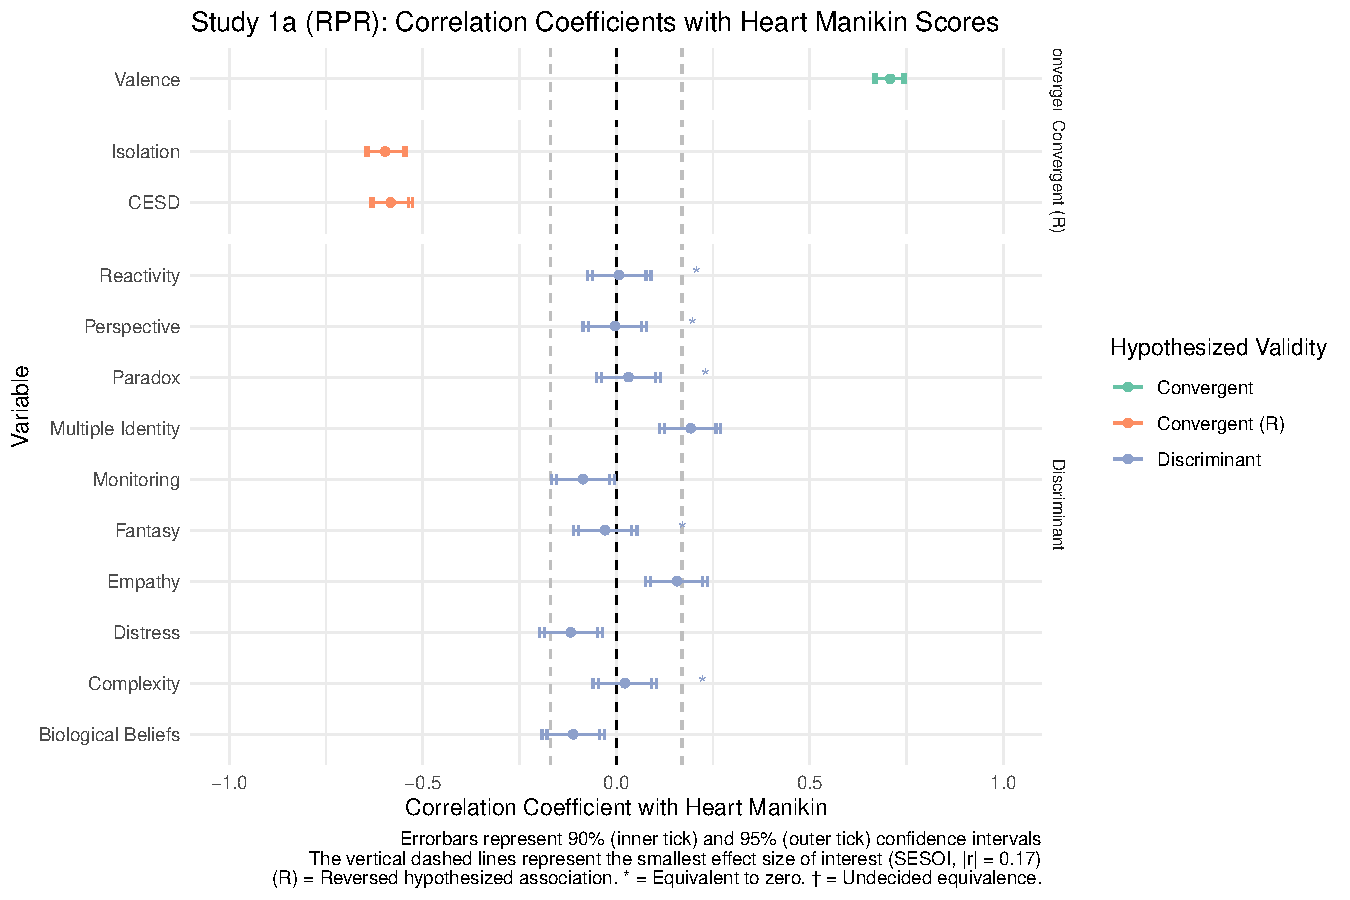
\includegraphics[keepaspectratio]{Sunami-Dissertation_files/figure-latex/s1a-forest-1.pdf}}
\caption{\label{fig:s1a-forest}Study 1a - Forestplot Showing Correlation Coefficients with Heart Manikin Scores.}
\end{figure}

\section{Study 1b (RAIv1)}\label{study-1b-raiv1}

This study was designed to test the relationship between interpersonal
distress and immune function (Jaremka, unpublished). Table \ref{tab:s1b-table}
shows a summary of the measures included in the study.

\begin{table}
\centering\centering
\caption{\label{tab:s1b-table}Summary of Measures for Study 1b}
\centering
\resizebox{\ifdim\width>\linewidth\linewidth\else\width\fi}{!}{
\begin{tabular}[t]{>{\raggedright\arraybackslash}p{5cm}>{\raggedright\arraybackslash}p{2cm}l>{\raggedright\arraybackslash}p{2cm}>{\raggedright\arraybackslash}p{3cm}}
\toprule
\textbf{Measure} & \textbf{Time} & \textbf{Construct} & \textbf{Validity} & \textbf{Citation}\\
\midrule
Self-Assessment Manikin - Valence & Time 1, 2, 3 & State valence & Con. & Bradley \& Lang, 1994\\
MacArthur Scale of Subjective Social Status & Time 1, 2, 3 & Subjective social status & Dis. & Adler et al., 2000\\
\addlinespace[0.3em]
\multicolumn{5}{l}{PROMIS—Short Form 8a}\\
\hspace{1em}Social Isolation & Time 1, 2, 3 & Social isolation & Con. (R) & Cella et al., 2019; Hahn et al., 2014\\
\hspace{1em}Emotional Support & Time 1, 2, 3 & Emotional support & Con. & Cella et al., 2019; Hahn et al., 2014\\
\hspace{1em}Informational Support & Time 1, 2, 3 & Informational support & Con. & Cella et al., 2019; Hahn et al., 2014\\
Couples Satisfaction Index & Time 1, 2, 3 & Romantic relationship quality & Con. & Funk \& Rogge, 2007\\
Inclusion of Other in Self Scale & Time 1, 2, 3 & Closeness between the self and the other person & Con. & Aron et al., 1992\\
Partner Responsiveness Scale & Time 1, 2, 3 & Romantic partner responsiveness & Con. & Gable et al., 2012\\
Relationship Conflict Scale & Time 1, 2, 3 & Conflicts in a romantic relationship & Con. (R) & Ad-hoc\\
Ostracism from Romantic Partner Scale & Time 1, 2, 3 & Ostracism from a romantic partner & Con. (R) & Ad-hoc\\
\addlinespace[0.3em]
\multicolumn{5}{l}{Abusive Behavior Inventory—Revised}\\
\hspace{1em}Psychological Abuse & Time 1, 2, 3 & Perpetration of psychological abuse against a romantic partner & Dis. & Postmus et al., 2015\\
\hspace{1em}Physical Abuse & Time 1, 2, 3 & Perpetration of physical abuse against a romantic partner & Dis. & Postmus et al., 2015\\
\addlinespace[0.3em]
\multicolumn{5}{l}{Controlling Behavior Scale—Modified}\\
\hspace{1em}Economic Control & Time 1, 2, 3 & Perpetration of economic control & Dis. & Graham-Kevan \& Archer, 2003\\
\hspace{1em}Threats & Time 1, 2, 3 & Perpetration of threats & Dis. & Graham-Kevan \& Archer, 2003\\
\hspace{1em}Intimidation & Time 1, 2, 3 & Perpetration of intimidation & Dis. & Graham-Kevan \& Archer, 2003\\
\hspace{1em}Emotional Control & Time 1, 2, 3 & Perpetration of emotonal control & Dis. & Graham-Kevan \& Archer, 2003\\
\hspace{1em}Isolation & Time 1, 2, 3 & Perpetration of isolation & Dis. & Graham-Kevan \& Archer, 2003\\
Modified Food Craving Questionnaire—Trait Version & Time 1, 2, 3 & Food craving & Dis. & Cepeda-Benito et al., 2000\\
Dietary Social Support Scale & Time 1, 2, 3 & Support from one's romantic partner about eating & Dis. & Ad-hoc\\
Body Image Questionnaire & Time 1, 2, 3 & Body image & Dis. & Ad-hoc\\
Godin Leisure-Time Exercise Questionnaire & Time 1, 2, 3 & Physical activity & Dis. & Godin, 2011; Godin \& Shephard, 1985\\
PROMIS Sleep Disturbance—Short Form 4a & Time 1, 2, 3 & Sleep disturbance & Dis. & Cella et al., 2019\\
Single-Item Narcissism Scale & Time 1, 2, 3 & Narcissism & Dis. & Konrath et al., 2014\\
Perceived Stress Scale & Time 1, 2, 3 & Perceived stress & Dis. & S. Cohen et al., 1983\\
\bottomrule
\multicolumn{5}{l}{\rule{0pt}{1em}\textit{Note.} Con. = Convergent Validity. Dis. = Discriminant Validity. (R) = Reverse association. }\\
\end{tabular}}
\end{table}

\subsection{Participants}\label{participants-1}

One-hundred and seven participants participated in the study.
Participants were eligible to participate if they were in a romantic
relationship at the beginning of the study. Participants were recruited
from the psychology participant pool at the University of Delaware. They
received partial course credits as compensation.

The dataset contained data from 121
participants. Participants were eligible to participate if they were in
a romantic relationship at the beginning of the study. Participants were
recruited from the psychology participant pool at the University of
Delaware. They received partial course credits as compensation. During
the data inspection, I found that two participants had duplicate data
points in the study One participant had 2 data points for the Visit 3 on
the same date but no data for Visit 2. For this participant, I
disregarded their data from later participation on that day. Another
participant had participated twice for Visit 1 on different dates. I
disregarded their data for the later participation for Visit 1.

\subsection{Procedure and Materials}\label{procedure-and-materials-1}

The study had three visits (Visits 1--3) with average intervals of
27.24 days between Visits 1 and 2, and
27.23 days between Visits 2 and 3,
respectively. In each visit, participants came to a group testing room
and answered all questionnaires. The Heart Manikin was identical to the
ones used in Study 1a. See Table \ref{tab:s1b-table} for the summary of
the measures and {[}Appendix{]} for detailed descriptions.

The following questionnaires included questions about their current
romantic partner: the Couples Satisfaction Index (\citeproc{ref-funkTestingRulerItem2007}{Funk \& Rogge, 2007}), the Inclusion of the
Other in the Self Scale to one's current romantic partner (\citeproc{ref-aronInclusionOtherSelf1992}{Aron et al., 1992}), the Partner
Responsiveness Scale (\citeproc{ref-gableApproachAvoidanceMotives2012}{Gable \& Impett, 2012}), the Relationship
Conflict Scale, the Ostracism from Romantic Partner Scale, the Abusive
Behavior Inventory-Revised (\citeproc{ref-postmusAbusiveBehaviorInventory2015}{Postmus et al., 2015}), the Controlling
Behavior Scale (\citeproc{ref-graham-kevanPhysicalAggressionControl2003}{Graham-Kevan \& Archer, 2003}), and the Dietary
Social Support Scale. In Visits 2 and 3, participants who are no longer
in a relationship with a partner previously reported answered about both
their relationship with a new romantic partner and their ex-partner.

\subsection{Results}\label{results-1}

For testing convergent validity, I constructed a mixed model that
predicted the Heart Manikin across time for each measure in Table
\ref{tab:s1b-table}. I included the fixed effects of Time (categorical;
1--3) and the scores of a given measure (centered). I first included the
random intercept and the random effect of Time. However, the model
failed to converge with the Time random effect, and thus I dropped the
Time random effect. Figure \ref{fig:s1b-forest} shows regression
coefficients for each measure predicting the Heart Manikin scores after
controlling for the fixed effect of Time.

\textbf{Convergent Validity}. Consistent with the predictions, all convergent
measures showed evidence for convergent validity: valence manikin
(\emph{B} = 0.57, \emph{SE} = 0.04, \emph{t} = 12.78, \emph{p} \textless{} .001), partner responsiveness
(\emph{B} = 0.39, \emph{SE} = 0.05, \emph{t} = 7.35, \emph{p} \textless{} .001), inclusion of the other in the self
(\emph{B} = 0.29, \emph{SE} = 0.06, \emph{t} = 5.11, \emph{p} \textless{} .001), informational support
(\emph{B} = 0.34, \emph{SE} = 0.05, \emph{t} = 6.20, \emph{p} \textless{} .001), emotional support
(\emph{B} = 0.43, \emph{SE} = 0.05, \emph{t} = 8.77, \emph{p} \textless{} .001), couples satisfaction
(\emph{B} = 0.44, \emph{SE} = 0.05, \emph{t} = 8.68, \emph{p} \textless{} .001), social isolation
(\emph{B} = -0.44, \emph{SE} = 0.05, \emph{t} = -7.95, \emph{p} \textless{} .001), partner ostracism
(\emph{B} = -0.38, \emph{SE} = 0.05, \emph{t} = -7.14, \emph{p} \textless{} .001), relationship conflict
(\emph{B} = -0.25, \emph{SE} = 0.05, \emph{t} = -4.78, \emph{p} \textless{} .001), and depression
(\emph{B} = -0.52, \emph{SE} = 0.05, \emph{t} = -10.07, \emph{p} \textless{} .001). These results suggest a strong support for
the convergent validity for the Heart Manikin.

\textbf{Discriminant Validity.} Out of the 13 measures for the discriminant
validity, 9 measures did not correlate with the Heart Manikin scores,
supporting the discriminant validity: sleep quality
(\emph{B} = 0.03, \emph{SE} = 0.06, \emph{t} = 0.56, \emph{p} = .578), socioeconomic status (\emph{B} = 0.13, \emph{SE} = 0.06, \emph{t} = 1.97, \emph{p} = .050),
psychological abuse perpetration
(\emph{B} = -0.17, \emph{SE} = 0.06, \emph{t} = -2.70, \emph{p} = .007), physical abuse perpetration
(\emph{B} = -0.02, \emph{SE} = 0.06, \emph{t} = -0.34, \emph{p} = .735), isolation control
(\emph{B} = -0.11, \emph{SE} = 0.06, \emph{t} = -1.86, \emph{p} = .064), intimidation control
(\emph{B} = -0.04, \emph{SE} = 0.05, \emph{t} = -0.73, \emph{p} = .464), emotional control
(\emph{B} = -0.09, \emph{SE} = 0.06, \emph{t} = -1.59, \emph{p} = .113), economic control
(\emph{B} = -0.09, \emph{SE} = 0.06, \emph{t} = -1.61, \emph{p} = .108), craving
(\emph{B} = -0.07, \emph{SE} = 0.07, \emph{t} = -1.02, \emph{p} = .310), and body image
(\emph{B} = -0.02, \emph{SE} = 0.07, \emph{t} = -0.27, \emph{p} = .786). Contrary to the prediction, 3 measures correlated with the
Heart Manikin: threats control (\emph{B} = -0.09, \emph{SE} = 0.06, \emph{t} = -1.59, \emph{p} = .113),
stress (\emph{B} = -0.42, \emph{SE} = 0.06, \emph{t} = -7.62, \emph{p} \textless{} .001), and narcissism
(\emph{B} = -0.14, \emph{SE} = 0.06, \emph{t} = -2.27, \emph{p} = .024).

For all coefficients with a \emph{p}-value greater than .05, I ran an
equivalence test to test if they were theoretically equivalent to zero
(Figure \ref{fig:s1b-forest}). Results showed that the correlation
coefficients with the measures of sleep quality, physical abuse,
intimidation, and body image were theoretically equivalent to zero
(using \textbar{}\emph{r}\textbar{} = 0.17). The correlation coefficients with the
measure of economic control, emotional control, and craving were not
equivalent to zero or different from zero, and thus I interpret the
results for these measures as ambiguous. Overall, the current results
suggest a moderate discriminant validity of the Heart Manikin scores,
especially against measures of sleep quality, physical abuse,
intimidation, and body image.

\begin{figure}
\centering
\pandocbounded{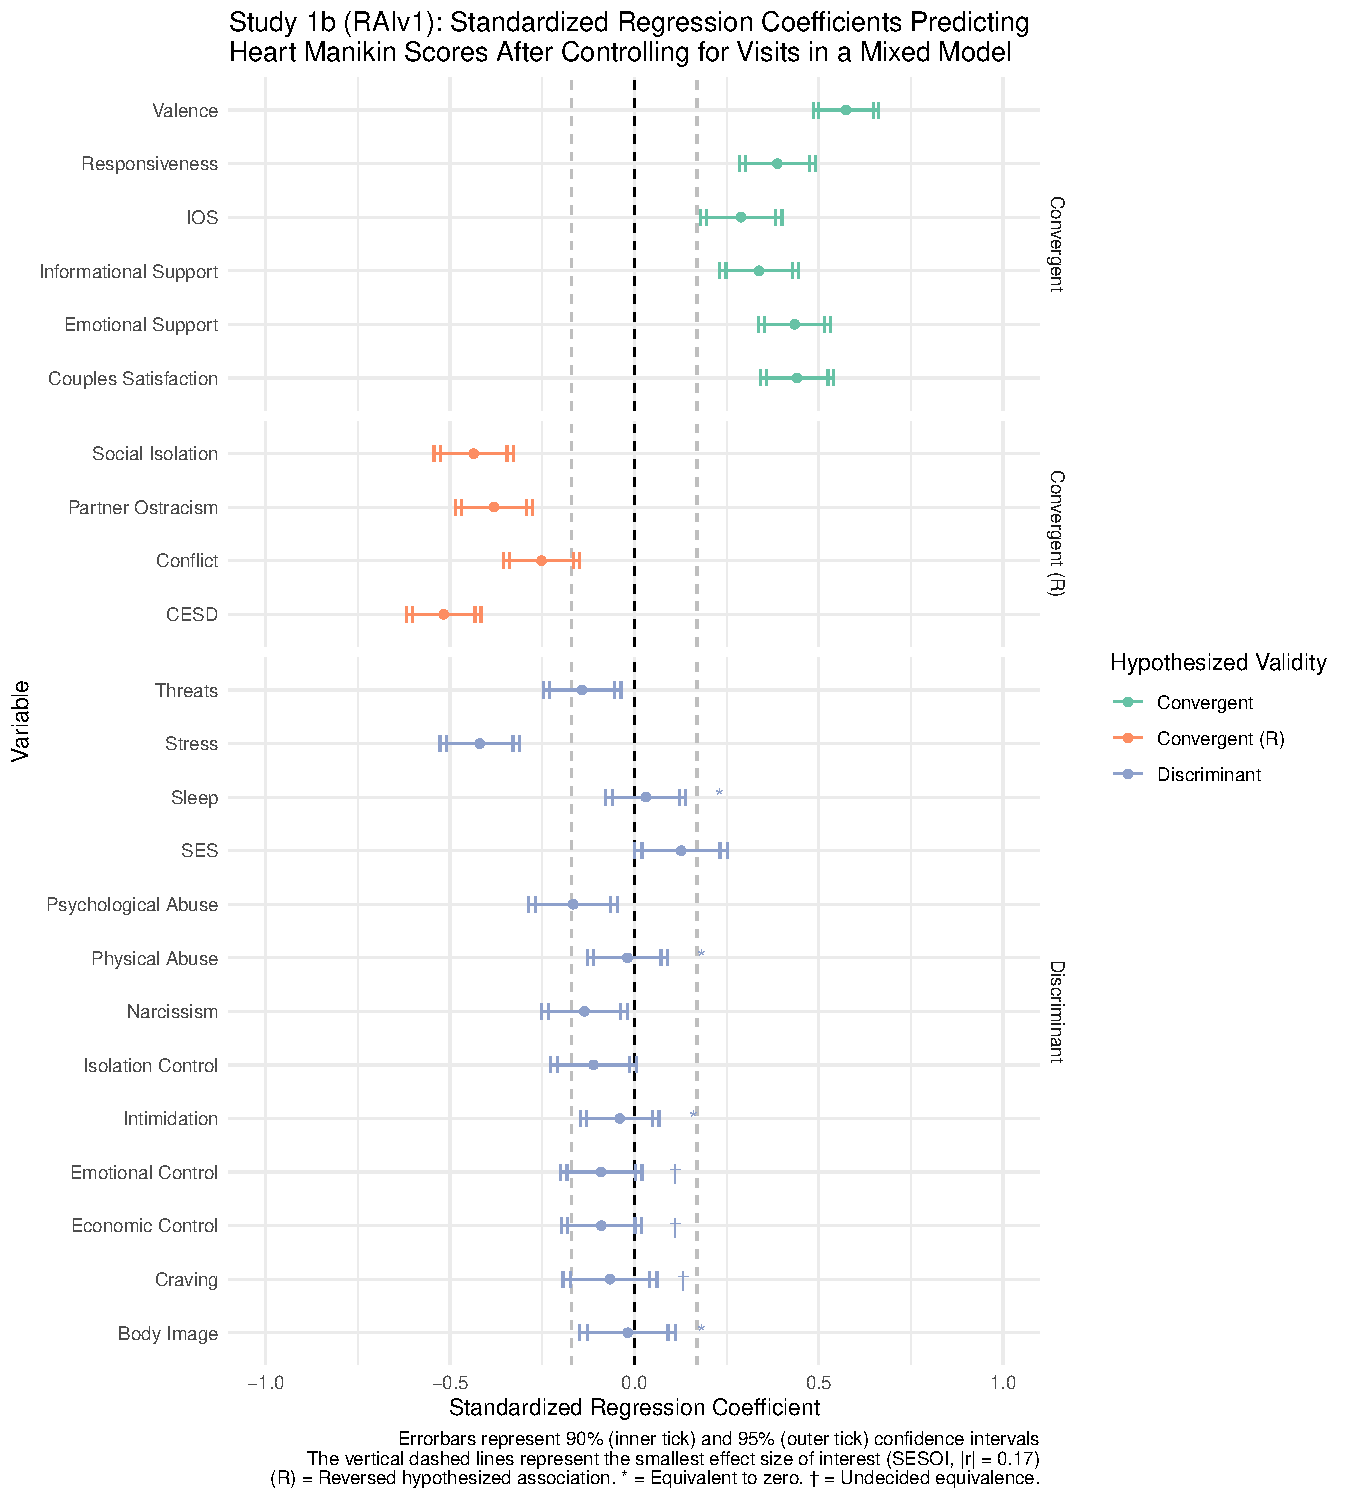
\includegraphics[keepaspectratio]{Sunami-Dissertation_files/figure-latex/s1b-forest-1.pdf}}
\caption{\label{fig:s1b-forest}Study 1b - Forestplot Showing Correlation Coefficients with Heart Manikin Scores}
\end{figure}

\textbf{Test-Retest Reliability.} To explore the test-retest reliability, I
constructed an unconditional mixed model predicting the Heart Manikin
scores over Time, and interpreted its intraclass correlation
(ICC) as a measure of reliability. The obtained ICC was
0.33 (average interval between visits =
36.3 days). The ICC indicates a poor reliability
according to the guideline (\citeproc{ref-kooGuidelineSelectingReporting2016}{Koo \& Li, 2016}). These results suggest that
participants reported different levels of Heart Manikin scores across
the visits. Note that the low reliability does not imply that the scale
performed well or poorly, since the Heart Manikin scale was meant to
measure fluctuations over time.

\section{Study 1c (ARv1)}\label{study-1c-arv1}

Study 1c was designed to test whether social rejection by a close other
threatens belonging more than social rejection by a stranger
(\citeproc{ref-nadzan2019}{Nadzan et al., 2019}). Table \ref{tab:s1c-table} summarizes the measures used
in the study.

\begin{table}
\centering\centering
\caption{\label{tab:s1c-table}Summary of Measures for Study 1c}
\centering
\resizebox{\ifdim\width>\linewidth\linewidth\else\width\fi}{!}{
\begin{tabular}[t]{>{\raggedright\arraybackslash}p{5cm}>{\raggedright\arraybackslash}p{2cm}l>{\raggedright\arraybackslash}p{2cm}>{\raggedright\arraybackslash}p{3cm}}
\toprule
\textbf{Measure} & \textbf{Time} & \textbf{Construct} & \textbf{Validity} & \textbf{Citation}\\
\midrule
\addlinespace[0.3em]
\multicolumn{5}{l}{Self-Assessment Manikin}\\
\hspace{1em}Valence & Times 1, 2, \& 3 & State valence & Con. & Bradley \& Lang, 1994\\
\hspace{1em}Arousal & Time 2 & State arousal & Dis. & Bradley \& Lang, 1994\\
\hspace{1em}Dominance & Time 2 & State dominance & Dis. & Bradley \& Lang, 1994\\
\addlinespace[0.3em]
\multicolumn{5}{l}{Modified Need-Threat Scale—Essay Version}\\
\hspace{1em}Belonging & Time 2 & Belonging & Con. & Williams, 2009\\
\hspace{1em}Self-Esteem & Time 2 & Self-esteem & Con. & Williams, 2009\\
\hspace{1em}Control & Time 2 & Control & Dis. & Williams, 2009\\
\hspace{1em}Meaningful Existence & Time 2 & Meaning existence & Dis. & Williams, 2009\\
MacArthur Scale of Subjective Social Status & Time 3 & Subjective social status & Dis. & Adler et al., 2000\\
\bottomrule
\multicolumn{5}{l}{\rule{0pt}{1em}\textit{Note.} Con. = Convergent Validity. Dis. = Discriminant Validity. (R) = Reverse association. }\\
\end{tabular}}
\end{table}

\subsection{Participants}\label{participants-2}

Two-hundred ninety-two participants were recruited from Amazon
Mechanical Turk (MTurk). Participants received \$1.50 for participation.

\subsection{Procedure and Materials}\label{procedure-and-materials-2}

The study was a 2 (Social Rejection: Rejection vs.~Acceptance) x 2
(Essay Target: Stranger vs.~Close Friend) design. Participants provided
informed consent and completed the Heart Manikin (Time 1) and the Time 1
measures (see Table \ref{tab:s1c-table}). Then, participants were
randomly assigned to one of the five essay conditions. In the stranger
rejection condition, participants wrote about a time when they felt
rejected by a stranger. In the close friend rejection condition,
participants wrote about a time when they felt rejected by a close
friend. In the stranger acceptance condition, participants wrote about a
time when they felt accepted by a stranger. In the close friend
acceptance, participants wrote about a time when they felt accepted by a
close friend. Participants wrote the essay for 5 minutes. After the
essay task, participants answered the Heart Manikin, the original
Self-Assessment Manikin, and the Need-Threat Scale at Time 2. Then,
participants indicated the characteristics of the person that they
described in the essay task, unrelated to the current scale validation.
Next, participants answered the Heart Manikin and the valence
Self-Assessment Manikin and further questions about the person in the
essay task at Time 3. Then, participants again answered the valence
Self-Assessment Manikin and the Heart Manikin, and the demographics at
Time 4 (\citeproc{ref-bradleyMeasuringEmotionSelfAssessment1994}{Bradley \& Lang, 1994}). See {[}Appendix{]} for the detailed
descriptions of these measures.

\subsection{Results}\label{results-2}

\textbf{Convergent and Discriminant Validities.} To test convergent
discriminant validities, I first examined the bivariate correlations
between the Heart Manikin and the included measures in Table
\ref{tab:s1c-table}. Detailed results are available in {[}Appendix{]}.
Here, I report the results with the socioeconomic status, since I detail
results for the other measures in the mixed models below. Contrary to
the prediction, the socioeconomic status scores correlated with the
Heart Manikin scores \emph{r}(288) = 0.18, \emph{p} = .002, 95\%CI {[}0.06, 0.29{]}, suggesting
that the Heart Manikin scores did not discriminate against the subjective
socioeconomic status.

To test convergent and discriminant validities after controlling for the
manipulations, I examined an association between the Heart Manikin
scores and Time 2 measures. To do so, I constructed regression models
predicting the Time 2 Heart Manikin scores for each Time 2 measure. I
included the following predictors in the model: the given Time 2
measure, Social Rejection (-0.5 = Rejection, 0.5 = Acceptance), Essay
Target (-0.5 = Stranger, 0.5 = Close Friend), and Social Rejection x
Essay Target. Results showed that all indicators for convergent validity
all predicted the Heart Manikin Scores: the valence manikin
(\emph{B} = 0.86, \emph{SE} = 0.03, \emph{t} = 24.85, \emph{p} \textless{} .001), self-esteem (\emph{B} = 0.57, \emph{SE} = 0.05, \emph{t} = 11.60, \emph{p} \textless{} .001),
belonging (\emph{B} = 0.79, \emph{SE} = 0.06, \emph{t} = 14.03, \emph{p} \textless{} .001), control
(\emph{B} = 0.33, \emph{SE} = 0.04, \emph{t} = 7.38, \emph{p} \textless{} .001), meaningful existence
(\emph{B} = 0.51, \emph{SE} = 0.05, \emph{t} = 10.08, \emph{p} \textless{} .001), and overall need-threat
(\emph{B} = 0.78, \emph{SE} = 0.05, \emph{t} = 15.26, \emph{p} \textless{} .001), supporting the convergent validity. Contrary
to the prediction, the discriminant validity indicators also co-varied
with the Heart Manikin as well: arousal (\emph{B} = 0.18, \emph{SE} = 0.04, \emph{t} = 4.62, \emph{p} \textless{} .001),
dominance (\emph{B} = 0.56, \emph{SE} = 0.04, \emph{t} = 15.64, \emph{p} \textless{} .001). See Figure
\ref{fig:s1c-T2reg-plot} for the forest plot.

\begin{figure}
\centering
\pandocbounded{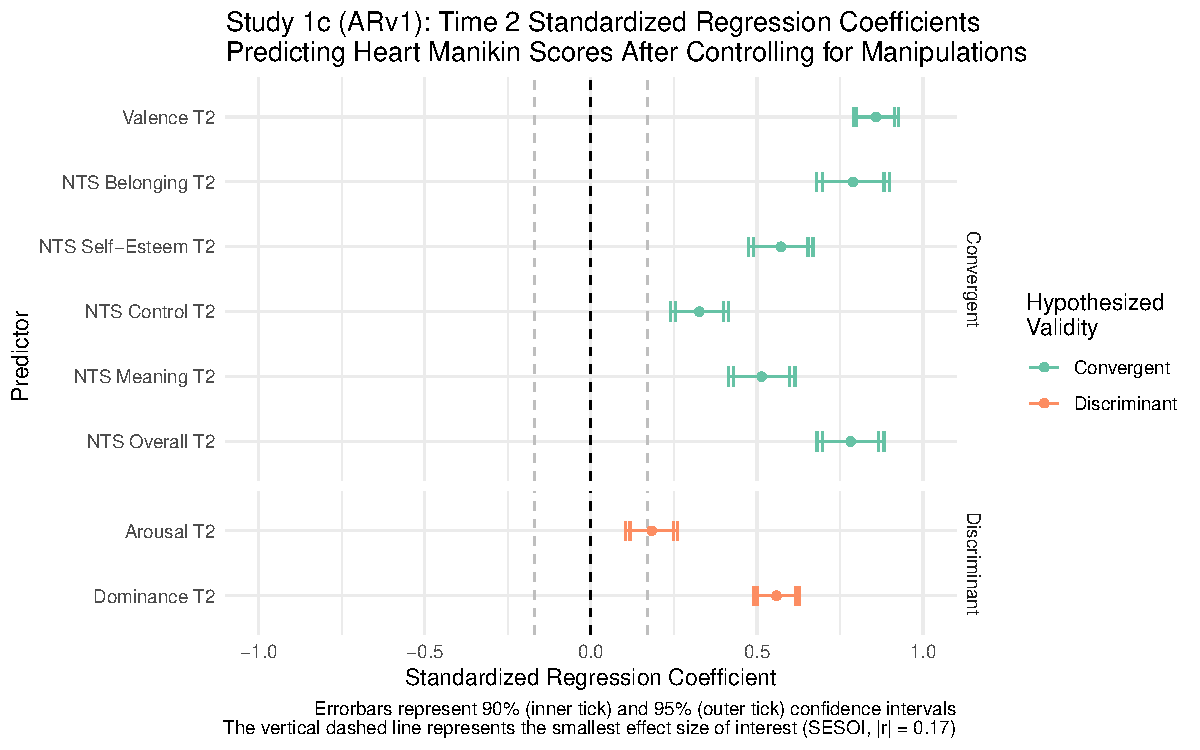
\includegraphics[keepaspectratio]{Sunami-Dissertation_files/figure-latex/s1c-T2reg-plot-1.pdf}}
\caption{\label{fig:s1c-T2reg-plot}Study 1c - Regression Coefficients at Time 2}
\end{figure}

Since the Heart Manikin and the Valence Manikin were measured over time, I created a linear mixed model to examine convergent and discriminant
validities of the Heart Manikin with the valence Self-Assessment Manikin
item across Times 1--3. I created a dummy variable (Grouping Dummy)
representing the four experimental groups in the study to facilitate
interpretation. The fixed predictors were Time, Valence Manikin,
Grouping Dummy, and Grouping Dummy x Time. Results showed that the
valence scores predicted the Heart Manikin scores
(\emph{B} = 0.70, \emph{SE} = 0.02, \emph{t} = 29.34, \emph{p} \textless{} .001) after controlling for the effects of
manipulations and Time. I interpret the results as a strong support for
the convergent validity between the Valence Manikin and the Heart
Manikin.

\textbf{Sensitivity to Experimental Manipulation.} To test the sensitivity of
the Heart Manikin scores to the social rejection manipulation, I ran a
Welch's \emph{t}-test comparing the rejection and acceptance conditions at
Time 2. Results showed that the rejected participants reported lower
Heart Manikin scores (\emph{M} = 2.97, \emph{SD} = 2.11) than the
accepted participatns (\emph{M} = 7.28, \emph{SD} = 1.95) at Time 2,
\emph{t}(286.8) = -18.06, \emph{p} \textless{} .001, \emph{d} = -2.12, 95\%CI {[}-2.41, -1.83{]} (see Figure
\ref{fig:s1c-sensitivity-plot}). Also, see Figure \ref{fig:appnedix-s1c-belonging-across-time} in {[}Appendix{]} for the Heart Manikin scores over time across conditions.

\begin{figure}
\centering
\pandocbounded{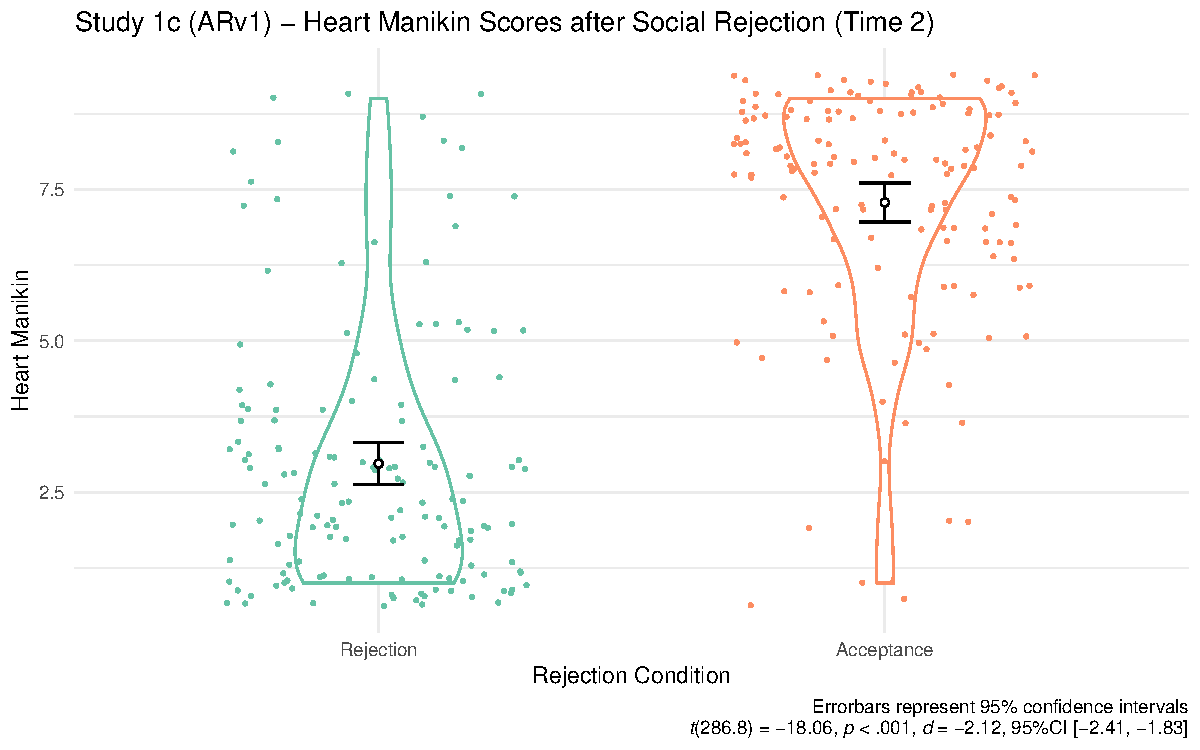
\includegraphics[keepaspectratio]{Sunami-Dissertation_files/figure-latex/s1c-sensitivity-plot-1.pdf}}
\caption{\label{fig:s1c-sensitivity-plot}Study 1c - Heart Manikin Scores across Rejection Conditions. Participants in the rejection condition reported lower Heart Manikin scores than those in the acceptance condition.}
\end{figure}

\textbf{Test-Retest Reliability.} To test test-retest reliability after
controlling for effects from experimental manipulations and time, I
calculated the ICC using the same linear mixed model for testing
convergent and discriminant validities without the valence Manikin term.
The obtained ICC was 0.44, which indicates poor
reliability according to the criteria (\citeproc{ref-kooGuidelineSelectingReporting2016}{Koo \& Li, 2016}). These results suggest
that the Heart Manikin scores changed across time points in the study
even after controlling for the effects of manipulation and time. Again, poor reliability does not imply the poor quality of the measure since the Heart Manikin should be able to capture fluctuations of belonging as a state measure.

\section{Study 1d (EVv1)}\label{study-1d-evv1}

This study was designed to test whether people who expect social
rejection show decreased cardiovascular threat response to social
rejection (Sunami et al., unpublished). The preregistration of the
original study is available at OSF (\url{https://osf.io/4xn52}) before data
collection. Table \ref{tab:s1d-table} summarizes the measures used in
the study.

\begin{table}
\centering\centering
\caption{\label{tab:s1d-table}Summary of Measures for Study 1d}
\centering
\resizebox{\ifdim\width>\linewidth\linewidth\else\width\fi}{!}{
\begin{tabular}[t]{>{\raggedright\arraybackslash}p{5cm}>{\raggedright\arraybackslash}p{2cm}l>{\raggedright\arraybackslash}p{2cm}>{\raggedright\arraybackslash}p{3cm}}
\toprule
\textbf{Measure} & \textbf{Time} & \textbf{Construct} & \textbf{Validity} & \textbf{Citation}\\
\midrule
\addlinespace[0.3em]
\multicolumn{5}{l}{Self-Assessment Manikin}\\
\hspace{1em}Valence & Times 1, 2, 3, \& 4 & State valence & Con. & Bradley \& Lang, 1994\\
\hspace{1em}Arousal & Times 1, 2, 3, \& 4 & State arousal & Dis. & Bradley \& Lang, 1994\\
\hspace{1em}Dominance & Times 1, 2, 3, \& 4 & State dominance & Dis. & Bradley \& Lang, 1994\\
Rosenberg Self-Esteem Scale & Time 1 & Self-esteem & Con. & Rosenberg, 1965a\\
Need for Closure Scale & Time 1 & Desire for an answer on any topic & Dis. & Roets \& Van Hiel, 2011\\
\addlinespace[0.3em]
\multicolumn{5}{l}{Modified Need-Threat Scale}\\
\hspace{1em}Belonging & Times 3 \& 4 & Belonging & Con. & Williams, 2009\\
\hspace{1em}Self-Esteem & Times 3 \& 4 & Self-esteem & Con. & Williams, 2009\\
\hspace{1em}Control & Times 3 \& 4 & Control & Dis. & Williams, 2009\\
\hspace{1em}Meaningful Existence & Times 3 \& 4 & Meaning existence & Dis. & Williams, 2009\\
Social Judgment Survey & Time 4 & Adherence to the traditional cultural values & Dis. & Proulx \& Heine, 2008; Rosenblatt et al., 1989\\
\bottomrule
\multicolumn{5}{l}{\rule{0pt}{1em}\textit{Note.} Con. = Convergent Validity. Dis. = Discriminant Validity. (R) = Reverse association. }\\
\end{tabular}}
\end{table}

\subsection{Participants}\label{participants-3}

Two-hundred thirty-seven participants were recruited for the study. A
debriefing coding procedure determined that 53 participants had either
had suspicions or figured out the hypothesis of the study, and thus they
were excluded. The final dataset consisted of 184 participants.

\subsection{Procedure and Materials}\label{procedure-and-materials-3}

Participants provided informed consent and wore electrocardiograph
electrodes and a blood pressure cuff to the participant for
cardiovascular recording, unrelated to the current scale validation.
Then, participants completed demographics, the Heart Manikin (Time 1),
and the Time 1 questionnaires in Table \ref{tab:s1d-table}. Then,
participants completed the participant desire manipulation similar to
Study 1c and answered the Self-Assessment Manikin and the Heart Manikin
(Time 2). Then, participants heard an audio recording ostensibly
recorded by their confederate, serving as a rejection manipulation. In
the rejection condition, the confederate said that the participant was
not their type. In the acceptance condition, the confederate said that
the participant was their type. After hearing the recording,
participants completed the modified Need-Threat Scale (\citeproc{ref-williamsOstracismTemporalNeedthreat2009}{Williams, 2009}),
the Self-Assessment Manikin, and the Heart Manikin (Time 3). Then,
participants completed a word-finding task with the confederate,
unrelated to the current validation, the Heart Manikin (Time 4), and the
Time 4 questionnaires in Table \ref{tab:s1d-table}. See
{[}Appendix{]} for the detailed descriptions of these measures.

\subsection{Results}\label{results-3}

\textbf{Convergent and Discriminant Validities.} To test convergent and
discriminant validities, I fist examined the bivariate correlations
between the Heart Manikin and the included measures (Table
\ref{tab:s1d-table}). Detailed results are available in
{[}Appendix{]}. I focus on the results of the non-repeated
measures (self-esteem and social judgment survey) here since the results
for the measures repeated throughout the study are reported in the mixed
models below. Results showed that the self-esteem scores at Time 1
significantly correlated with the Heart Manikin scores at Time 1
(\emph{r}(239) = 0.57, \emph{p} \textless{} .001, 95\%CI {[}0.48, 0.65{]}), supporting the hypothesized
convergent validity. The social judgment survey scores at Time 4 did not
correlate with the Heart Manikin scores at Time 4
(\emph{r}(235) = -0.05, \emph{p} = .466, 95\%CI {[}-0.17, 0.08{]}), supporting the
hypothesized discriminant validity.

For the Self-Assessment Manikin items measured across Times 1--4, I
constructed a linear mixed model predicting the Heart Manikin. I
included the fixed effect of a measured score (centered), Time
(categorical), Confederate Desire (.5 = high, -.5 = low), Rejection (.5
= rejection, -.5 = acceptance), Time x Confederate Desire, Time x
Rejection, Confederate Desire x Rejection, and Time x Confederate Desire
x Rejection. I interpret the coefficient for the measured score as
evidence for convergent or discriminant validity after controlling for
the manipulations and timing of measurements. Results showed that
valence scores predicted the Heart Manikin scores
(\emph{B} = 0.42, \emph{SE} = 0.02, \emph{t} = 18.49, \emph{p} \textless{} .001, Figure \ref{fig:s1d-mixed-plot}), consistent with
the hypothesized convergence. Contrary to the prediction, arousal
(\emph{B} = 0.18, \emph{SE} = 0.03, \emph{t} = 6.08, \emph{p} \textless{} .001) and dominance (\emph{B} = 0.41, \emph{SE} = 0.03, \emph{t} = 14.81, \emph{p} \textless{} .001)
also predicted the Heart manikin scores in these models.

\begin{figure}
\centering
\pandocbounded{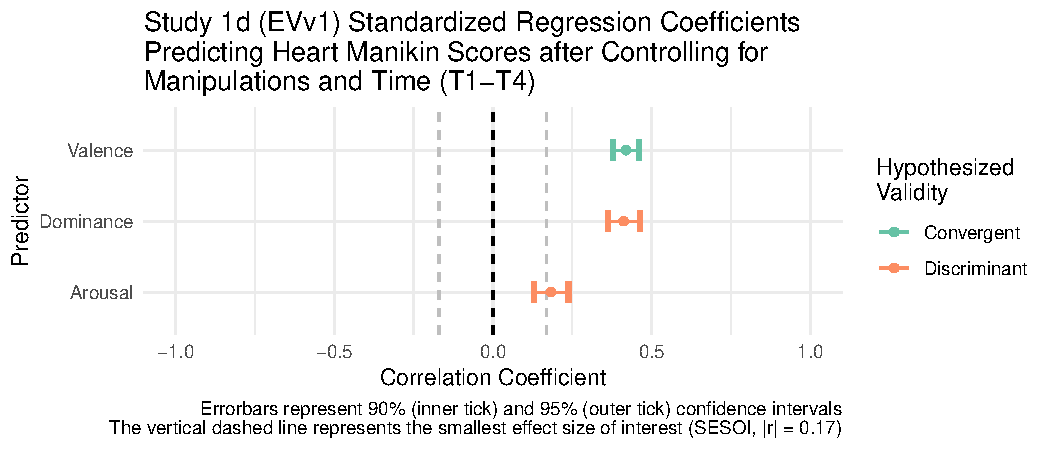
\includegraphics[keepaspectratio]{Sunami-Dissertation_files/figure-latex/s1d-mixed-plot-1.pdf}}
\caption{\label{fig:s1d-mixed-plot}Study 1d - Standardized Regression Coefficients Predicting Heart Manikin Scores after Controlling for Manipulations and Time}
\end{figure}

\textbf{Sensitivity to Experimental Manipulation.} To test the sensitivity of
the Heart Manikin to experimental manipulation, I ran Welch's \emph{t}-test
comparing the rejected and accepted participants at Time 3. Results
showed that rejected participants (\emph{M} = 5.77, \emph{SD} = 2.01)
reported lower Heart Manikin scores than accepted participants
(\emph{M} = 6.88, \emph{SD} = 1.39, \emph{t}(205.5) = 4.95, \emph{p} \textless{} .001; see
Figure \ref{fig:s1d-sensitivity-plot}). Also, see Figure \ref{fig:appendix-s1e-belonging-plot} in {[}Appendix{]} for the Heart Manikin scores over time across conditions.

\begin{figure}
\centering
\pandocbounded{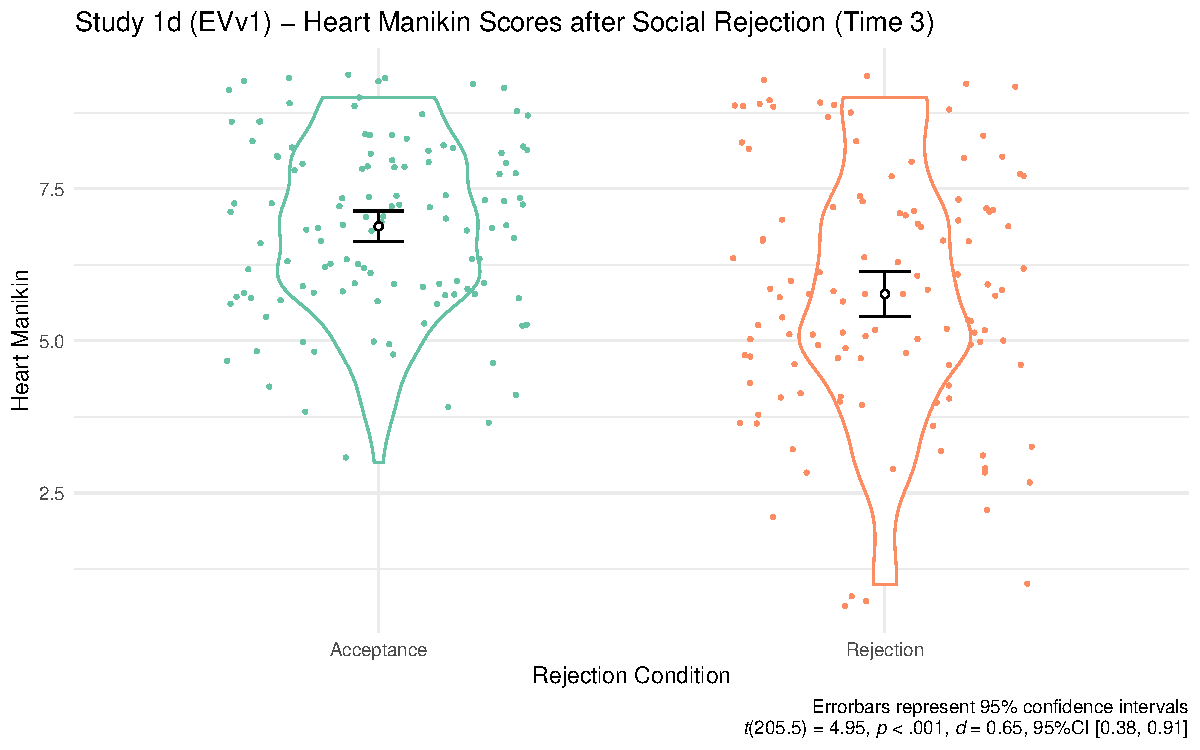
\includegraphics[keepaspectratio]{Sunami-Dissertation_files/figure-latex/s1d-sensitivity-plot-1.pdf}}
\caption{\label{fig:s1d-sensitivity-plot}Study 1d - Sensitivity of Heart Manikin to Rejection Manipulation. Rejected participants reported lower Heart Manikin scores than accepted participants.}
\end{figure}

\textbf{Test-Retest Reliability.} To test test-retest reliability, I created
a linear mixed model predicting the Heart Manikin scores. The fixed
predictor was the same as the model above testing convergent and
discriminant validity except that the model did not include the measured
score predictor. Results showed that the calculated ICC was
0.75, suggesting a
moderate-to-good reliability of the Heart Manikin measure across Times 1
to 4.

Across Studies 1a, 1b, 1c, and 1d, I validated the Heart Manikin
measure. In the next study, I continued the validation. In addition, I
aimed to examine the effectiveness of the rejection manipulation that I
planned to use for the subsequent studies.

\section{Study 1e (NPSv2)}\label{study-1e-npsv2}

The original research question of this study was to test the
reconnection hypothesis---whether the prospect of fulfilling belonging
influences social responses to rejection (\citeproc{ref-sunamiDoesProspectFulfilling2019}{Sunami et al., 2019}). The study was
pre-registered before data collection (\url{https://osf.io/xpr6b}). Table
\ref{tab:s1e-table} shows a summary of the measures included in this
study.

\begin{table}
\centering\centering
\caption{\label{tab:s1e-table}Summary of Measures for Study 1e}
\centering
\resizebox{\ifdim\width>\linewidth\linewidth\else\width\fi}{!}{
\begin{tabular}[t]{>{\raggedright\arraybackslash}p{5cm}>{\raggedright\arraybackslash}p{2cm}l>{\raggedright\arraybackslash}p{2cm}>{\raggedright\arraybackslash}p{3cm}}
\toprule
\textbf{Measure} & \textbf{Time} & \textbf{Construct} & \textbf{Validity} & \textbf{Citation}\\
\midrule
\addlinespace[0.3em]
\multicolumn{5}{l}{Self-Assessment Manikin}\\
\hspace{1em}Valence & Times 1, 2, 3, 4, 5, \& 6 & State valence & Con. & Bradley \& Lang, 1994\\
\hspace{1em}Arousal & Times 1, 2, 3, 4, 5, \& 6 & State arousal & Dis. & Bradley \& Lang, 1994\\
\hspace{1em}Dominance & Times 1, 2, 3, 4, 5, \& 6 & State dominance & Dis. & Bradley \& Lang, 1994\\
\addlinespace[0.3em]
\multicolumn{5}{l}{Experiences in Close Relationships Scale—Short Form}\\
\hspace{1em}Avoidance & Time 1 & Attachment avoidance & Con. (R) & Wei et al., 2007\\
\hspace{1em}Anxiety & Time 1 & Attachment anxiety & Con. (R) & Wei et al., 2007\\
Fear of Negative Evaluation Scale—Brief Version & Time 1 & Apprehension in expecting negative judgment from others & Con. (R) & Leary, 1983\\
Rosenberg Self-Esteem Scale & Time 1 & Self-esteem & Con. & Rosenberg, 1965a\\
MacArthur Scale of Subjective Social Status & Time 1 & Subjective social status & Dis. & Adler et al., 2000\\
Rejection Sensitivity Questionnaire—Short Version & Time 1 & Rejection sensitivity & Con. (R) & Downey \& Feldman, 1996; Romero-Canyas et al., 2010\\
\addlinespace[0.3em]
\multicolumn{5}{l}{Modified Need-Threat Scale}\\
\hspace{1em}Belonging & Time 3 & Belonging & Con. & Williams, 2009\\
\hspace{1em}Self-Esteem & Time 3 & Self-esteem & Con. & Williams, 2009\\
\hspace{1em}Control & Time 3 & Control & Dis. & Williams, 2009\\
\hspace{1em}Meaningful Existence & Time 3 & Meaning existence & Dis. & Williams, 2009\\
\bottomrule
\multicolumn{5}{l}{\rule{0pt}{1em}\textit{Note.} Con. = Convergent Validity. Dis. = Discriminant Validity. (R) = Reverse association. }\\
\end{tabular}}
\end{table}

\subsection{Procedure and Materials}\label{procedure-and-materials-4}

The study was a 2 (Participant Desire; low vs.~high) x 2 (Confederate
Desire, low vs.~high) x 2 (Social Rejection, rejection vs.~control)
design. I only describe the procedure and measures relevant to the
current validation in detail here. More detailed descriptions are
available in a published study (\citeproc{ref-sunamiDoesProspectFulfilling2019}{Sunami et al., 2019}). On Day 1, participants
answered the Heart Manikin and the Time 1 questionnaires (see Table
\ref{tab:s1e-table}). Then, participants completed the manipulation for
the participants' desire to affiliate with the confederate (Participant
Desire) and answered the Heart Manikin and the Self-Assessment Manikin
(Time 2). Participants then completed the manipulation of the
confederate's desire to affiliate with the participant (Confederate
Desire) and answered the Modified Need-Threat Scale (\citeproc{ref-nadzan2019}{Nadzan et al., 2019}; \citeproc{ref-williamsOstracismTemporalNeedthreat2009}{Williams, 2009}), the Self-Assessment Manikin, the Heart Manikin (Time 3).
The manipulations for Participant Desire and Confederate Desire are
unrelated to the current validation, and details are available in a
published study (\citeproc{ref-sunamiDoesProspectFulfilling2019}{Sunami et al., 2019}).

\subsection{Participants}\label{participants-4}

This study was a two-day study (separated by 6.22 days on average), with 674 participants on Day 1 and 605
participants on Day 2. A debriefing coding procedure determined that 67
participants had either had suspicions or figured out the hypothesis of
the study, and thus they were excluded. The final analytic sample
consisted of 538 participants.

\textbf{Rejection Essay Manipulation.} On Day 2, participants completed the
Self-Assessment Manikin and the Heart Manikin (Time 4). Then,
participants completed the social rejection manipulation essay where
they were randomly assigned to either a rejection condition or a control
condition (adapted from \citeproc{ref-twengeIsnItFun2003}{Twenge \& Campbell, 2003}). All participants spent
5 minutes writing the essay. In the rejection condition, participants
wrote about a time when they felt rejected by a person or a group of
their own age (excluding romantic rejection) for 5 minutes:

\begin{quote}
We'd like you to write about a time when you felt rejected or excluded
by a person or a group about your own age. By ``felt rejected'' we mean
that you felt like a person or persons did not value you or your
relationship. That is, describe an episode in which you wanted to
spend time with or do something with someone, and that person or
persons did not let you do so. Make sure to be as detailed as possible
and describe not only what happened, but also how you felt. If the
rejection is by an organized group of people, make sure it is of
people about your same age. For example, being rejected from a college
or job is NOT what we are asking about. Please do NOT describe a
romantic rejection, if possible.
\end{quote}

In the control condition, participants wrote about their yesterday
morning:

\begin{quote}
We'd like you to write about your morning yesterday. Please describe
what you did yesterday morning. Make sure to be as detailed as
possible and describe not only what happened, but also how you felt.
\end{quote}

After naming their social surrogate and non-social surrogate video
games, participants completed the social rejection essay task that I
validate in Study 1e (\citeproc{ref-sunamiDoesProspectFulfilling2019}{Sunami et al., 2019}). All participants
wrote about a time when they felt rejected by a person or a group of
their own age (excluding romantic rejection) for 5 minutes:

\begin{quote}
We'd like you to write about a time when you felt rejected or excluded
by a person or a group about your own age. By ``felt rejected'' we mean
that you felt like a person or persons did not value you or your
relationship. That is, describe an episode in which you wanted to
spend time with or do something with someone, and that person or
persons did not let you do so. Make sure to be as detailed as possible
and describe not only what happened, but also how you felt. If the
rejection is by an organized group of people, make sure it is of
people about your same age. For example, being rejected from a college
or job is NOT what we are asking about. Please do NOT describe a
romantic rejection, if possible.
\end{quote}

After writing the essay, participants answered the Self-Assessment
Manikin and the Heart Manikin, and the Need-Threat Scale (Time 5),
completed experimental tasks unrelated to the current study (\citeproc{ref-sunamiDoesProspectFulfilling2019}{Sunami et al., 2019}), and again
answered the Self-Assessment Manikin and the Heart Manikin (Time 6).

\subsection{Results}\label{results-4}

\textbf{Convergent and Discriminant Validities.} To test convergent and
discriminant validities, I first examined bivariate correlations between
the Heart Manikin scores and scores of the measures (Table
\ref{tab:s1e-table}). I focus on the results for the subjective
socioeconomic status here since the results for the other repeated
measures are reported in more detail in the mixed model analyses below.
Results showed that the subjective
socioeconomic status did not correlate with the Heart
Manikin (\emph{r}(536) = 0.05, \emph{p} = .289, 95\%CI {[}-0.04, 0.13{]}). An equivalence test
showed that the 90\% confidence interval of this correlation coefficient
fell within the smallest effect size of interest (\textbar{}\emph{r}\textbar{} = 0.17), suggesting that the
observed coefficient was theoretically equivalent to zero
(\emph{r}(536) = 0.05, \emph{p} = .289, 90\%CI {[}-0.03, 0.12{]}). These results support the
hypothesized discriminant validity of the Heart Manikin against
subjective socioeconomic status

For the Self-Assessment Manikin scores measured over Times 1--6 and the
Need-Threat scores over Times 3 and 5, I constructed a linear mixed
model predicting the Heart Manikin scores. I created a dummy categorical
variable (Grouping Dummy) representing the four experimental conditions
for Participant Desire and Confederate Desire to reduce the number of
interactions in the model (coded as 0-3). I included the fixed effects
of the measured scores (centered), Time (categorical), Dummy for the
Participant Desire and Confederate Desire conditions (categorical),
social rejection (rejected = -.5, control = .5), Grouping Dummy,
Grouping Dummy x Rejection, Rejection x Time, Rejection x Grouping
Dummy, Rejection x Time x Grouping Dummy. Results showed that the
Valence Manikin, belonging, self-esteem, control, and meaningful
existence scores predicted the Heart Manikin scores after controlling
for the manipulations and time, supporting the hypothesized convergent
validity as expected (Valence: \emph{B} = 0.35, \emph{SE} = 0.01, \emph{t} = 24.02, \emph{p} \textless{} .001; Belonging:
\emph{B} = 0.57, \emph{SE} = 0.03, \emph{t} = 21.00, \emph{p} \textless{} .001; Control:
\emph{B} = 0.30, \emph{SE} = 0.03, \emph{t} = 10.72, \emph{p} \textless{} .001; Meaningful Existence:
\emph{B} = 0.46, \emph{SE} = 0.03, \emph{t} = 17.62, \emph{p} \textless{} .001; Overall Need-Threat:
\emph{B} = 0.57, \emph{SE} = 0.03, \emph{t} = 21.64, \emph{p} \textless{} .001). However, the Arousal and Dominance Manikin
scores also predicted the Heart Manikin scores, contrary to the
expectation (Arousal: \emph{B} = 0.11, \emph{SE} = 0.02, \emph{t} = 7.04, \emph{p} \textless{} .001; Dominance:
\emph{B} = 0.34, \emph{SE} = 0.02, \emph{t} = 21.07, \emph{p} \textless{} .001). Overall, the mixed model analyses showed a
strong support for the convergent validity of the Heart Manikin, but no
support for the discriminant validity with the Arousal and Dominance
Manikins.

\begin{figure}
\centering
\pandocbounded{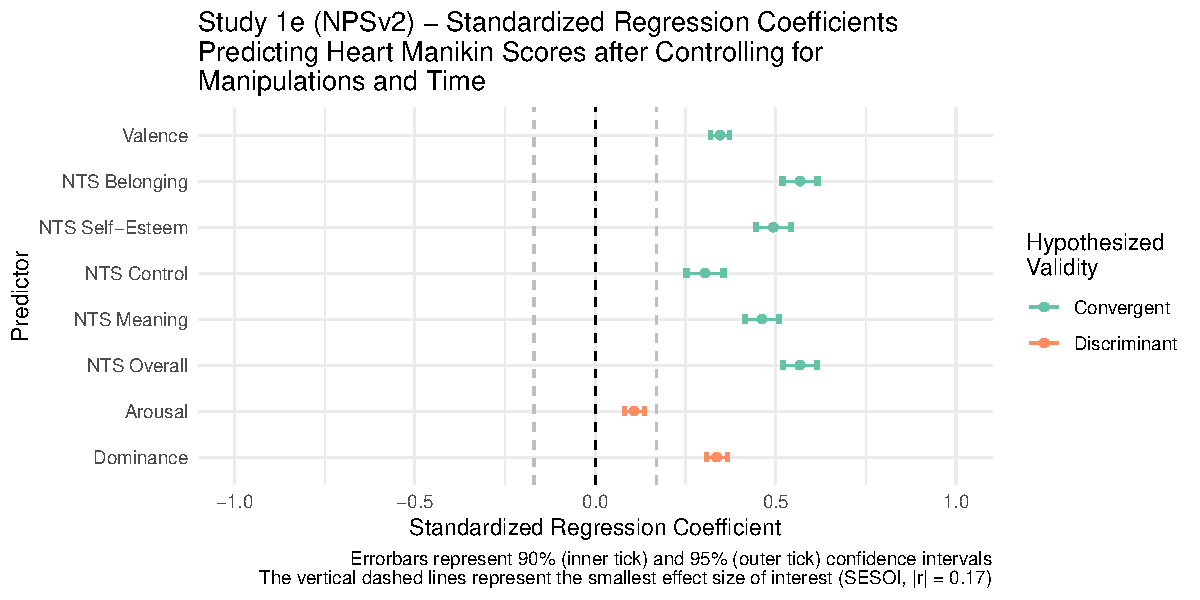
\includegraphics[keepaspectratio]{Sunami-Dissertation_files/figure-latex/s1e-mixed-plot-1.pdf}}
\caption{\label{fig:s1e-mixed-plot}Study 1e - Forestplot Showing Regression with Heart Manikin Scores from the Mixed Model}
\end{figure}

\textbf{Sensitivity to Experimental Manipulation.} To test the sensitivity of
the Heart Manikin scores to a social rejection manipulation, I ran a
Welch's \emph{t}-test comparing the rejected and control groups following the
social rejection manipulation at Time 5 (right after the social rejection manipulation). The
rejected participants (\emph{M} = 6.47, \emph{SD} = 1.88) reported lower
Heart Manikin scores than the control participants
(\emph{M} = 6.78, \emph{SD} = 1.55, \emph{t}(518.8) = 2.11, \emph{p} = .036 ,
\emph{d} = 0.18, 95\%CI {[}0.01, 0.35{]}, see Figure \ref{fig:s1e-belonging-plot}).

\begin{figure}
\centering
\pandocbounded{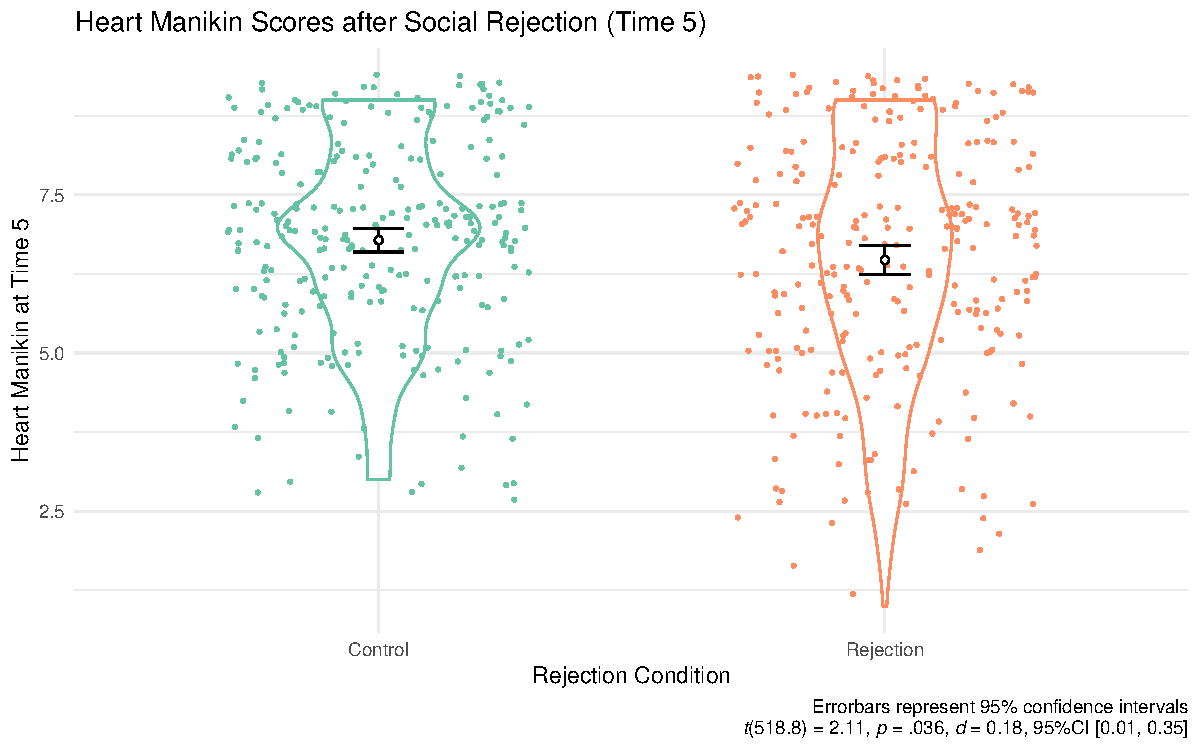
\includegraphics[keepaspectratio]{Sunami-Dissertation_files/figure-latex/s1e-belonging-plot-1.pdf}}
\caption{\label{fig:s1e-belonging-plot}Study 1e - Heart Manikin Scores.}
\end{figure}

\textbf{Test-Retest Reliability.} To test test-retest reliability, I created
a linear mixed model predicting the Heart Manikin scores across
measurements. I included the same fixed effects as the model above testing the convergent and discriminant validity except that the
model did not include a predictor for a measured score. The calculated
ICC was 0.72, indicating a
moderate test-retest reliability after controlling for the effects of
the experimental manipulations.

\textbf{Effectiveness of Rejection Manipulation on Belonging.} To test the
effectiveness of the rejection manipulation on belonging, I performed a
series of Welch's \emph{t}-tests on the belonging subscale of the Need-Threat
Scale at Time 5 (Figure \ref{fig:s1e-NTS-plot}). Results showed that
participants in the rejection condition reported lower belonging
(\emph{M} = 79.13, \emph{SD} = 16.68) than those in the control condition
(\emph{M} = 82.04, \emph{SD} = 14.18,
\emph{t}(521.6) = 2.18, \emph{p} = .030, \emph{d} = 0.19, 95\%CI {[}0.02, 0.36{]}), indicating that the manipulation
was effective. See Figure \ref{fig:appendix-s1e-belonging-plot} in {[}Appendix{]} for the Heart Manikin scores over time across conditions.

\begin{figure}
\centering
\pandocbounded{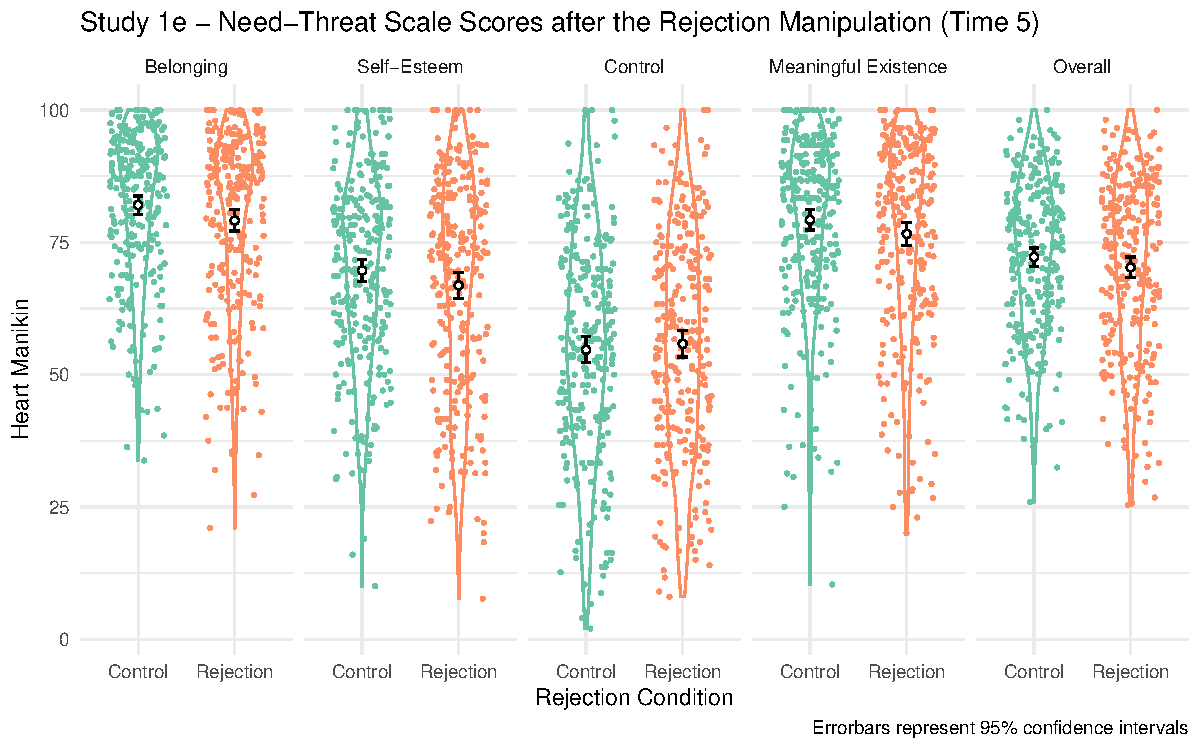
\includegraphics[keepaspectratio]{Sunami-Dissertation_files/figure-latex/s1e-NTS-plot-1.pdf}}
\caption{\label{fig:s1e-NTS-plot}Study 1e - Need-Threat Scores Across Rejection and Control Conditions}
\end{figure}

I also ran Welch's \emph{t}-tests on other subscales of the
need-threat scale (self-esteem, control, and meaningful existence).
Results showed that rejected participants and control participants did
not report different levels of self-esteem, control, meaningful
existence, or the overall need-threat (self-esteem:
\emph{t}(524.4) = 1.71, \emph{p} = .088, \emph{d} = 0.15, 95\%CI {[}-0.02, 0.32{]}, control:
\emph{t}(536.0) = -0.63, \emph{p} = .531, \emph{d} = -0.05, 95\%CI {[}-0.22, 0.12{]}, meaning:
\emph{t}(527.8) = 1.78, \emph{p} = .075, \emph{d} = 0.15, 95\%CI {[}-0.02, 0.32{]}, overall need-threat:
\emph{t}(524.9) = 1.46, \emph{p} = .145, \emph{d} = 0.13, 95\%CI {[}-0.04, 0.30{]}). These results suggest that although the
rejection manipulation was effective in inducing lowered belonging, it
may not have been effective in lowering self-esteem, control, meaningful
existence, or overall fundamental need.

\section{Deciding a Rejection Manipulation for Subsequent Studies}\label{deciding-a-rejection-manipulation-for-subsequent-studies}

The effect size for the rejection manipulation of Study 1e was small
(\emph{d} = 0.18, 95\%CI {[}0.01, 0.35{]}). Also, the manipulation did not lower the
fundamental needs that usually track with the rejection manipulations in
the other studies (\citeproc{ref-williams2005}{Williams et al., 2005}). These results raised a concern about
the effectiveness of the rejection manipulation. Since I plan to use the
rejection manipulation without a control or acceptance condition, I
wanted to ensure the effectiveness of the manipulation. These results
implied that the manipulation used in Study 1e may not be optimal to
use for the purpose of this dissertation.

Study 1c included a different version of the essay rejection
manipulation, which showed a large effect size when compared with an
acceptance condition (\emph{d} = -2.12, 95\%CI {[}-2.41, -1.83{]}). However, I cannot
directly compare this effect size with the effect size obtained in Study
1e since Study 1c contrasted rejection with acceptance condition. To
make the effect size comparable as possible, I ran a pared t-test
comparing the the Heart Manikin scores before and after the rejection
manipulation (Times 1 vs.~2) only among the rejected participants.
Results showed that rejected participants reported lower belonging at
Time 2 than Time 1 (\emph{t}(145.0) = 17.49, \emph{p} \textless{} .001, \emph{d} = 1.45, 95\%CI {[}1.21, 1.68{]}). The
obtained effect size in Study 1c's manipulation was nearly
8
times larger than the effect size of Study 1e's manipulation. Although
the two effect sizes may not be directly comparable due to the
difference in the study designs (within-subject for Study 1c and between
for Study 1e), the magnitude of the difference was concerning given that
both studies shared the same outcome measure (Heart Manikin). Overall,
these results strongly indicated that Study 1c's manipulation was more
effective in manipulating belonging than Study 1e. To ensure the
effectiveness of the rejection manipulation used in Studies 2 and 3, I
have decided to use the rejection procedure in Study 1c instead of Study
1e's procedure.

\section{Discussion}\label{discussion}

Across 5 studies (1200+ participants), I examined the convergent validity, discriminant
validity, test-retest reliability, and
sensitivity to social rejection manipulation the Heart Manikin. Overall, I found a strong support for the convergent validity and sensitivity to social rejection manipulation. On the other hand, I found mixed evidence for discriminant validity.

\textbf{Convergent Validity.} The Heart Manikin scores correlated with the
hypothesized convergent measures: belonging, self-esteem, control, and
meaningful existence needs (Studies 1c, 1d, and 1e), social isolation
(Study 1a), interpersonal relationship quality and conflict (Study 1b),
depression (Studies 1a and 1b), and valence (Studies 1a, 1b, 1c, 1d, and
1e). The current results strongly support that the Heart Manikin scores
converge with belonging and its associated measures.

\textbf{Discriminant Validity.} I found mixed results for the discriminant
validity of the Heart Manikin scores. On one hand, the Heart Manikin
scores showed evidence for discrimant validity against interpersonal
reactivity, paradoxical mindset, self-monitoring, integrative
complexity, sleep quality, physical abuse perpetration, intimidation
perpetartion, emotional control, economic control, food craving, and
body image. On the other hand, the Heart Manikin scores correlated with
the measures of multiple identity (Study 1a), social monitoring (Study
1a), beliefs in biological differences between Black and White people
(Study 1a), perpetration of threats against one's partner (Study 1b),
stress (Study 1b), narcissism (Study 1b), arousal (Studies 1c and 1e),
and dominance (Studies 1c and 1e). The discriminant validity against the
socioeconomic status was particularly mixed. In Studies 1b and 1e, I
found that the Heart Manikin discriminated against socioeconomic status.
In Study 1c, the Heart Manikin scores correlated with socioeconomic status, contrary to the prediction.

Although this is result-dependent reasoning, I realize that some of
these discriminant measures can converge with belonging. For example,
people with multiple identities could report more belonging since they
belong to multiple groups, people with higher social monitoring can
cultivate social connections easily, and people who do not threaten
their partner experience more loving interactions. I do not have
post-hoc explanations for why people with higher Heart Manikin scores
reported lower narcissism, less biological beliefs in differences
between Black and White people, and higher socioeconomic status.

Note that some of the observed associations can be attributed to Type I
error. For example, I found the association between the
socioeconomic status and the Heart Manikin in Study 1c, but not Studies 1b and 1e,
adding to the possibility of Type I error. In contrast, this possibility
of Type I error is less likely for arousal and dominance since I observed the associations for these
measures across two studies (Studies 1c and 1e).

\textbf{Test-Retest Reliability.} I observed test-retest reliability of
0.33 in Study 1b (measured 3 times separated by
36.3days on average),
0.44 in Study 1c (measured 3 times in a 15-minute
study), 0.75 in Study 1d (EVv1) (measured 4 times
in an 1-hour study) , and 0.72 in Study 1e
(measured 6 times in two 30-minute experimental studies separated by 6.22
days on average). The reliability ranged from poor to moderate, which
suggests that the Heart Manikin scores vary relatively considerably
across time, and thus may be suitable to be used as a state measure,
rather than a trait measure.

\textbf{Sensitivity to Social Rejection Manipulation.} In Studies 1c, 1d, and
1e, I tested the sensitivity to social rejection of the Heart Manikin
scores. The results showed that rejected participants reported lower
Heart Manikin scores across the studies. I conclude that the Heart
Manikin scores are sensitive to social rejection manipulation.

Overall, I suggest that Study 1 supported the convergent validity of
the Heart Manikin. The results for the discriminant validity was mixed.
I suggest that the Heart Manikin scores track
belonging well but do not necessarily distinguish belonging from other
constructs, including general stress, arousal, and dominance.
Given the promising results of the convergent validity,
I decided to use the Heart Manikin sores as key outcome variable in my subsequent studies.

The current study has constraints on generality. First, I used existing
data for the current validation. As a result, the sample sizes of the
studies were not based on a proper power analysis, making the results
susceptible to Type I and Type II errors. In addition, the measures in
the studies were not a priori selected to validate the Heart Manikin.
Second, the sample demographics were limited to undergraduate students
from an introductory psychology course at the University of Delaware.
Most participants were young and predominantly White, and thus I do not
know if the current results generalize to other populations with different
characteristics.
Despite the shortcomings, the current
study included 65 measures from 5 studies, and thus maximizing the
generality across measures and samples.

\chapter{Study 2: Can Recalling A Game with Social Surrogates Replenish Belonging?}\label{study-2-can-recalling-a-game-with-social-surrogates-replenish-belonging}

In this study, I contrasted video games with social surrogates (social surrogacy games) and those without (non-social surrogacy games) to examine if socially rejected people can replenish their belonging by remembering about a time playing a social surrogacy game vs.~a non-social surrogacy game. I modeled the procedure after an existing study investigating the effect of recalling a favorite vs.~non-favorite TV program on belonging after social rejection (\citeproc{ref-derrickSocialSurrogacyHow2009}{Derrick et al., 2009}, Study 3). Based on the social surrogacy hypothesis, I expected that rejected people who write about a social surrogacy video game would have higher belonging than those who write about a non-social surrogacy video game (Hypothesis 1).

\section{Method}\label{method}

\subsection{Sample Size Rationale}\label{sample-size-rationale}

To my knowledge, only one study tested whether recalling a media with or without social surrogates replenished belonging following social rejection (\citeproc{ref-derrickSocialSurrogacyHow2009}{Derrick et al., 2009}, Study 2). I did not use the effect size reported in this study for the following reasons. First, an effect size observed in a single study can be upwardly biased and unreliable (\citeproc{ref-lakensEquivalenceTestsPractical2017}{Lakens, 2017}; \citeproc{ref-laneEstimatingEffectSize1978}{Lane \& Dunlap, 1978}). Second, the media used in the original study was a TV program, not a video game, and thus the effect size may not be compatible.

Instead, I again used an average effect size estimate (\emph{r} = .21) across 474 meta-analyses as a starting point (\citeproc{ref-richardOneHundredYears2003}{Richard et al., 2003}) consistent with the procedure in Study 1. As mentioned, the safeguarded target effect size was Cohen's \emph{d} = 0.35. With 90\% power to reduce Type II error and 5\% alpha by convention, I plan to recruit 344 (172 per group) participants to detect the effect size of \emph{d} = 0.35 in a two-group design. I also considered this effect size as the smallest effect size of interest for the equivalence test. Any effect sizes smaller than \emph{d} = 0.35 was considered theoretically equivalent to zero in the context of the current study.

\subsection{Participants}\label{participants-5}

I recruited 426 participants from Prolific in total (Age: \emph{M} = 24.92, \emph{SD} = 7.33; 133 women, 287 men, and 6 not identifying as a woman or man). The final analytic sample after exclusions was 359. See Exclusions, Data Stopping Rule section below. Participants received \$2.40 (\$9.60 per hour rate x 15 minutes) for compensation. Only participants who had regularly played both video games with social surrogates and video games without social surrogates were eligible to participate. In a screening survey, participants first saw the description of single-player video games, and indicate (a) whether they played any video games with social surrogates and without social surrogates and (b) whether they enjoyed playing these video games:

\begin{quote}
Some video games can be played by yourself (a single-player mode), where you are not playing with other players. Other games have the option to play with other players (a multiplayer mode). We want you to exclusively focus on games that have a single-player mode. There are lots of different genres of single-player games.
\end{quote}

\begin{quote}
One genre is single-player role-playing games (RPGs). These games always have stories that progress throughout the game, and they usually have non-player characters (NPCs). Classic examples of this type of game are Mass Effect, Zelda, Final Fantasy (single-player version), and Witcher. Question: Have you ever played a video game from this genre? (Yes/No)
\end{quote}

\begin{quote}
IF YES: Do you enjoy playing video games from this genre? (Yes/No)
\end{quote}

\begin{quote}
Other video games do not have these features, meaning they lack a story or non-player characters (NPCs) and focus on the mechanics of completing a specific task like a puzzle, beating the clock while completing a task, or earning points by doing a task. Classic examples are Poker, Solitaire, Tetris, or sports games that do not have teams like Pro Skater (skateboarding), Lonely Mountains Downhill (off-road biking). Question: Have you ever played a video game from these genres? (Yes/No)
\end{quote}

\begin{quote}
IF YES: Do you enjoy playing video games from these genres? (Yes/No)
\end{quote}

Only participants who indicated yes to all questions were invited to participate in the study. For social surrogate games, I focused on RPGs because people form strong parasocial relationships with other non-player characters, and people become immersed in the social worlds and stories presented in RPGs.

\subsection{Procedure}\label{procedure}

Participants accessed an online survey, signed an informed consent, and completed the demographics. Participants also completed the baseline Heart Manikin (Time 1) and the original Self-Assessment Manikin. I included the original Self-Assessment Manikin items to reduce demand characteristics. Participants again saw the screener questions above. Instead of yes or no question, participants were asked to nominate one game from the genres described (i.e., ``Please name one game from this genre that you enjoyed the most'' for social surrogate games, ``Please name one game from these genres that you enjoyed the most'' for non-social surrogate games).

After naming their social surrogate and non-social surrogate video games, participants completed the social rejection essay task that was found effective in Study 1c. All participants wrote about a time when they felt rejected by a close other for 3 minutes:

\begin{quote}
Everyone has different types of relationships in their lives -- some of which are very close relationships whereas others are not as close. Think of all of the people in your life that you feel very close to, and bring to mind a time when you felt rejected or excluded by one of those people. By ``felt rejected'' we mean that you felt this person did not value you or your relationship. In the space below, spend 3 minutes writing about this experience (i.e., a time when you felt rejected or excluded by a close other). Make sure to be as detailed as possible and describe not only what happened but also how you felt during the experience. Please continuously write for the entire 3 minutes, even if you have to repeat yourself. Do not worry about grammar or sentence structure, it is more important that you write about the experience continuously for 3 minutes.
\end{quote}

After completing the social rejection essay, participants were randomly assigned to either the social surrogacy condition or the non-social surrogacy condition in the video game essay task, adapted from the previous study (\citeproc{ref-derrickSocialSurrogacyHow2009}{Derrick et al., 2009}). Participants spent 5 minutes writing the essay. In the social surrogacy condition, participants wrote about a time they played the video game with social surrogates nominated earlier:

\begin{quote}
Please think of a time when you played X {[}the social surrogacy video game{]}. Who is (are) your favorite non-player character(s)? What was the story of the game you are thinking of? What happened to your favorite non-player character(s)? How did the gameplay make you feel? Write about everything you can remember about this particular game. Be as detailed as possible and try to relive playing the game in your mind as you write this description. Please continuously write for the entire 3 minutes, even if you have to repeat yourself. Do not worry about grammar or sentence structure, it is more important that you write about the experience continuously for 3 minutes.
\end{quote}

In the non-social surrogate video game condition, participants wrote about a time they played the non-social surrogate game:

\begin{quote}
Please think of a time when you played X {[}the non-social surrogacy game{]}. What was (were) the goal(s)? What tasks were you supposed to complete? What was involved in completing the tasks? How did the gameplay make you feel? Write about everything you can remember about this particular game. Be as detailed as possible and try to relive playing the game in your mind as you write this description. Please continuously write for the entire 3 minutes, even if you have to repeat yourself. Do not worry about grammar or sentence structure, it is more important that you write about the experience continuously for 3 minutes.
\end{quote}

After completing the video game essay, participants completed the Heart Manikin and the original Self-Assessment Manikin (Time 2). Next, participants answered whether they interacted with the non-player characters in their essay (Yes or No). If they answered yes, they completed the modified Inclusion of Self in Other Scale (\citeproc{ref-aronInclusionOtherSelf1992}{Aron et al., 1992}) and the modified Parasocial Interaction---Process Scale (\citeproc{ref-schrammPSIProcessScalesNew2008}{Schramm \& Hartmann, 2008}). Then, participants completed the modified Single-Item Immersion Scale (\citeproc{ref-reysenInitialValidationReliability2019}{Reysen et al., 2019}), the modified Narrative Engagement Scale (\citeproc{ref-busselleMeasuringNarrativeEngagement2009}{Busselle \& Bilandzic, 2009}), the on-the-fly measure of social world, and the Enjoyment Subscale of the Game User Experience Satisfaction Scale {[}GUESS; Phan et al. (\citeproc{ref-phanDevelopmentValidationGame2016}{2016}){]}. Participants also answered the year that they regularly played the games, frequency, and duration of play in open-ended questions for the game in their essay. These responses were used for exploratory analyses (``When did you play game X?'' {[}Example answer: 2010-2012{]}; ``How frequently and long did you play the game X?'' {[}Example answer: 2 times a week for 6 months{]}). Finally, participants completed the attention check.

\subsection{Measures}\label{measures}

The Heart Manikin was identical to the one used in Study 1a.

\textbf{Modified Inclusion of Self in Other Scale---Parasocial Relationship with Characters.} I adapted the Inclusion of Other in the Self Scale (\citeproc{ref-aronInclusionOtherSelf1992}{Aron et al., 1992}) used in Study 1 to measure the strength of the parasocial relationship players formed with the non-player characters in the video games in the essay. I modified the labels for the circles as ``Self'' and ``NPCs''. Participants chose a circle that best represents the relationship they experienced with the non-player characters in their essay.

\textbf{Modified Parasocial Interaction---Process Scale.} I adapted the Parasocial Interaction---Process Scale (12 items) (\citeproc{ref-schrammPSIProcessScalesNew2008}{Schramm \& Hartmann, 2008}) to measure the levels of parasocial interactions experienced in gameplay described in the essay task. I modified the language to refer to multiple characters in the video game (e.g., ``I carefully followed the behavior of the non-player characters in the game'') instead of a single character. Participants indicated their answers on a 5-point scale (0 = Not at all, 4 = Very much). Cronbach's alpha for the current sample was 0.80. I included this scale as an exploratory measure.

\textbf{Modified Single-Item Immersion Scale.} The single-item immersion scale is a one-item measure of immersion to media (\citeproc{ref-reysenInitialValidationReliability2019}{Reysen et al., 2019}). I modified the scale to measure immersion to the social world in the video game described in the essay task. Participants indicated their agreement with the statement, ``While playing the game X {[}the game title they wrote an essay about{]} I felt completely immersed'' on a 7-point scale (-3 = Strongly disagree, 3 = Strongly agree). I used the raw response score as an index. The scale has an adequate test-retest reliability (r = .71, over a semester) and convergent validity with other measures of immersion (\citeproc{ref-reysenInitialValidationReliability2019}{Reysen et al., 2019}).

\textbf{Modified Narrative Engagement Scale.} The Narrative Engagement Scale is a 12-item measure of engagement with a story (\citeproc{ref-busselleMeasuringNarrativeEngagement2009}{Busselle \& Bilandzic, 2009}). The original statements in the scale refer to narrative engagement in a TV program or a film (e.g., ``At times during the \emph{program}, the story world was closer to me than the real world.''). I modified the statements to make references to the gameplay (e.g., ``At times during the \emph{gameplay}, the story world was closer to me than the real world.''). Participants indicated their agreement on these statements on a 7-point scale (-3 = Strongly disagree, 3 = Strongly agree). I used the aggregated average as an index. Cronbach's alpha for the current sample was 0.60. The scale showed criterion validity with measures of media enjoyment (\citeproc{ref-busselleMeasuringNarrativeEngagement2009}{Busselle \& Bilandzic, 2009}).

\textbf{On-the-Fly Measure of Social World.} I created an on-the-fly measure of the social world to measure how much people experienced the social world in the game. The scale had four items: ``The video game presented stories that I immersed myself in'', ``The video game presented another social world where I felt like I belonged'', ``The video game had a social narrative that told an engaging story'', and ``I found myself getting''lost'' in the game's story''. Participants indicated their agreement on these statements on a 7-point scale (-3 = Strongly disagree, 3 = Strongly agree). Cronbach's alpha for the current sample was 0.88. I calculated an aggregated average as an index of social world. The scale's validity and reliability are unknown.

\textbf{Enjoyment Subscale of the Game User Experience Satisfaction Scale (GUESS).} I adapted the Enjoyment Subscale of the Game User Experience Satisfaction Scale {[}GUESS; Phan et al. (\citeproc{ref-phanDevelopmentValidationGame2016}{2016}){]}. The subscale has 5 items that refer to enjoyment in playing a video game: ``I think the game is fun'', ``I enjoy playing the game'', ``I feel bored while playing the game'' (reversed), ``I am likely to recommend this game to others'', and ``If given the chance, I want to play this game again''. Participants indicated their agreement to the statements on a 7-point scale (-3 = Strongly Disagree, 3 = Strongly Disagree) about the game that they wrote an essay about. I used the aggregated average as an index of enjoyment. Cronbach's alpha for the current sample was 0.82.

\textbf{Attention Check.}Participants were asked about the nature of the first essay: ``In today's study, you were asked to write a couple of essays. In the first essay, what were you asked to write about?'' Participants can answer this question as ``about a time I felt rejected'', ``about a time I felt accepted'', and ``about my morning yesterday''. I marked participants as failing the attention check if they indicated that they were asked to write about a time they felt accepted or about their morning yesterday.

Participants also indicated the type of video game that they wrote in the video game essay: ``In today's study, which type of the video games were you asked to write an essay about?'' Participants can answer this question as (1) ``role-playing games (RPGs)'', (2) ``video games without a storyline or NPCs'', or (3) ``unsure''. I marked participants as failing the attention check if (a) they indicated that they wrote about video games without a storyline or NPCs in the social surrogate video game condition, (b) they indicated they wrote about RPGs in the non-social surrogate video game condition, or (c) they indicated \emph{unsure}.

\textbf{Debriefing Questions.} I included two open-ended debriefing questions to gather qualitative information about participants' experience in the study. One question asked about the purpose of the study (``During the study, did you wonder about the purpose of the study or procedures? If so, what did you think the study was about?''). Another question asked participants to write in anything that they wanted to share (``Is there anything you'd like to share with us about your experience in this study? Please use the space below to explain your answers to any of the previous questions, or to provide any feedback.''). I presented these questions in a counterbalanced order. I included these questions as exploratory without a pre-registered analysis plan.

\subsection{Exclusion, Data Quality Check, and Stopping Rule}\label{exclusion-data-quality-check-and-stopping-rule}

I excluded any participants who did not complete the entire study or failed the attention check (12 failed the rejection essay attention check, 12 failed the video game attention check). To ensure that participants nominated video games according to the instructions, three coders checked the nominated video game titles and mark each participant as following the instructions or not (yes or no). If a participant nominated either of their social or non-social video games incorrectly, the participant were marked as not following the instructions. I calculated the interrater agreement among the coders, and the two coders with the highest agreement determined the initial codes, and the third coder resolved the discrepancies. This procedure excluded 51 (12.14\%) participants (overall interrater agreement: 80.60). I stopped recruitment when the sample size reached the target sample size after exclusions.

\section{Results}\label{results-5}

\textbf{Main Analysis.} I performed Welch's \emph{t}-test to compare the post-essaay Heart Manikin scores (Time 2) between the participants who wrote about the social surrogacy video game and those who wrote about the non-social surrogacy video game. Based on the social surrogacy hypothesis, I expected that participants who wrote about the social surrogacy video game would have higher belonging than those who wrote about the non-social surrogacy video game. Contrary to this expectation, participants who wrote about the social surrogacy game (\emph{M} = 6.37, \emph{SD} = 1.88) reported similar levels of belonging compared with those who wrote about a non-surrogacy game (\emph{M} = 6.27, \emph{SD} = 1.94, \emph{t}(355.1) = 0.49, \emph{p} = .624, see Figure \ref{fig:heart2}).

\begin{figure}
\centering
\pandocbounded{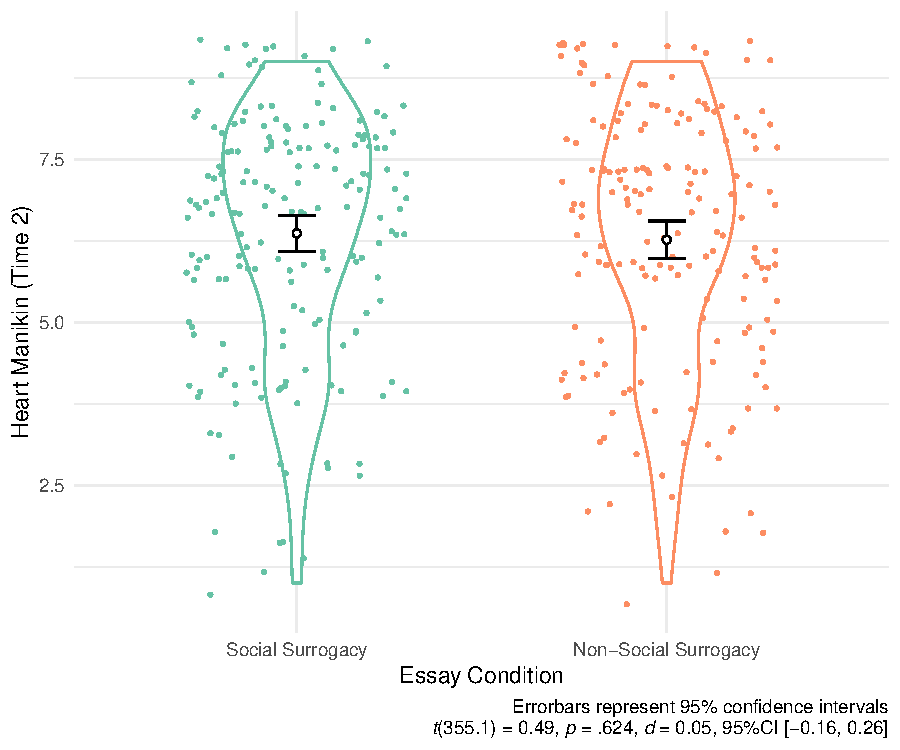
\includegraphics[keepaspectratio]{Sunami-Dissertation_files/figure-latex/heart2-1.pdf}}
\caption{\label{fig:heart2}Study 2 - Heart Mankin Scores at Time 2 across Essay Conditions}
\end{figure}

Since the obtained \emph{p}-value was greater than .05, I performed the two one-sided tests of equivalence to examine if the obtained effect size was theoretically equivalent to zero (Lakens, 2017). I considered the effect size of \emph{d} = 0.35 as the smallest effect size of interest (SESOI). Thus, any effect sizes between \emph{d} = -0.35 and \emph{d} = 0.35 are theoretically equivalent to zero. To compare the observed effect size with the SESOI, I calculated the 90\% confidence interval around the observed effect size. Then, I compared this confidence interval with \emph{d} = -0.35 and \emph{d} = 0.35. I set the confidence to 90\% because the TOST procedure involves two one-sided tests each with a 5\% alpha (Lakens, 2017). The observed effect size estimate fell within -0.35 \textless{} \emph{d} \textless{} 0.35, and its observed confidence interval did not include \emph{d} = -0.35 or \emph{d} = 0.35 (\emph{d} = 0.05, 90\%CI {[}-0.12, 0.23{]}). Thus, I consider the observed effect size as theoretically equivalent to zero.

\textbf{Probing Effectiveness of Rejection Induction.} I probed the effectiveness of the rejection induction by comparing the Heart Manikin scores at Times 1 and 2 among the participants in the non-social surrogate game condition. If the rejection induction was effective, I expected that these participants would report lower belonging after the rejection induction (Time 2) compared with the baseline (Time 1). To test this possibility, I ran a paired-samples \emph{t}-test comparing the Heart Manikin scores at Times 1 vs.~2. Contrary to the prediction, participants in the non-surrogate essay condition reported similar levels of belonging at Times 1 (baseline, \emph{M} = 6.18, \emph{SD} = 1.97) and 2 (after two essays, \emph{M} = 6.27, \emph{SD} = 1.94), \emph{t}(175.0) = -1.01, \emph{p} = .312, see Figure \ref{fig:heart12}. Given the non-significant results, I performed the TOST consistent with the main analysis. Results indicated that the obtained confidence interval fell within the SESOI (\emph{d} = -0.04, 90\%CI {[}-0.15, 0.08{]}), and thus I consider the effect size as theoretically equivalent to zero. Note that this analysis does not conclude the effectiveness of the rejection induction. The rejection induction could have been effective at first, but participants might have replenished their belonging due to passing of time--a point that I explore in more detail in the Discussion section below.

\begin{figure}
\centering
\pandocbounded{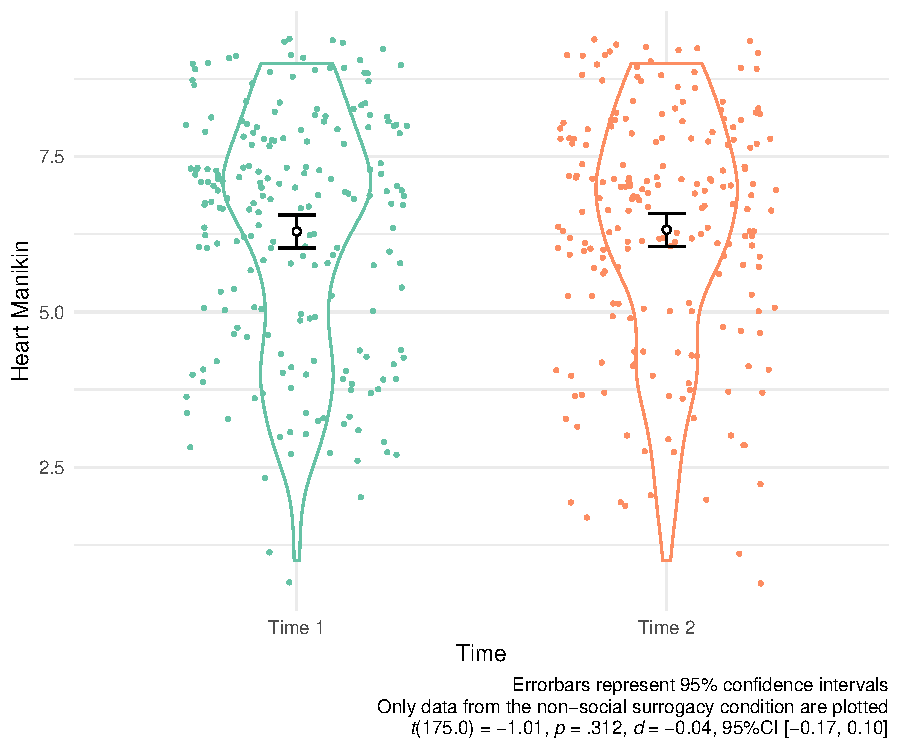
\includegraphics[keepaspectratio]{Sunami-Dissertation_files/figure-latex/heart12-1.pdf}}
\caption{\label{fig:heart12}Study 2 - Heart Mankin Scores at Times 1 \& 2 among the Non-Surrogate Group}
\end{figure}

\textbf{Exploratory Manipulation Check.} To explore the effectiveness of the video game essay manipulation in inducing parasocial relationships, I used the combination of two sources of information: the yes/no question about the presence of parasocial interaction (i.e., whether participants interacted with the non-player characters in their essay), and the modified Inclusion of Self in the Other Scale (Aron et al., 1992). I coded each participant into three groups as follows. If a participant indicated that they did not interact with non-player characters (answering no to the yes/no question), they were coded as ``did not interact with non-player characters'' (Group 1). If they indicated yes, and they scored 0 on the modified Inclusion of Self in the Other Scale (\citeproc{ref-aronInclusionOtherSelf1992}{Aron et al., 1992}), they were coded as ``interacted with non-player characters but did not form parasocial relationships'' (Group 2). All others received a code ``interacted with non-player characters and formed parasocial relationships'' (Group 3). I ran a two-way chi-square test (Essay: Social Surrogacy vs.~Non-Social Surrogacy x Groups: 1, 2, vs.~3) to examine whether those in the social surrogacy essay condition (vs.~the non-social surrogacy condition) indicated they interacted with an NPC (Group 2) and formed parasocial relationships (Group 3) rather than they did not interact with non-player characters (Group 1). This procedure allowed participants to indicate that they did not interact with non-player characters, a response option not available in the modified Inclusion of Self in the Other Scale (\citeproc{ref-aronInclusionOtherSelf1992}{Aron et al., 1992}). Participants reported different levels of parasocial relationships across the essay conditions (X2(2, \emph{N} = 359) = 184.93, \emph{p} \textless{} .001, see Figure \ref{fig:exp-mosaic}). Among the participants who wrote about a social surrogacy game, the majority reported forming a parasocial relationship with an NPC (88.52\%), than not forming a parasocial relationship (3.28\%), or not interacting with an NPC at all (8.2\%). In contrast, among the participants who wrote about a non-social surrogacy game, the majority reported not interacting with an NPC at all (75.57\%), followed by not forming a parasocial relationship (6.82), or forming a parasocial relationship with an NPC (17.61\%).

\begin{figure}
\centering
\pandocbounded{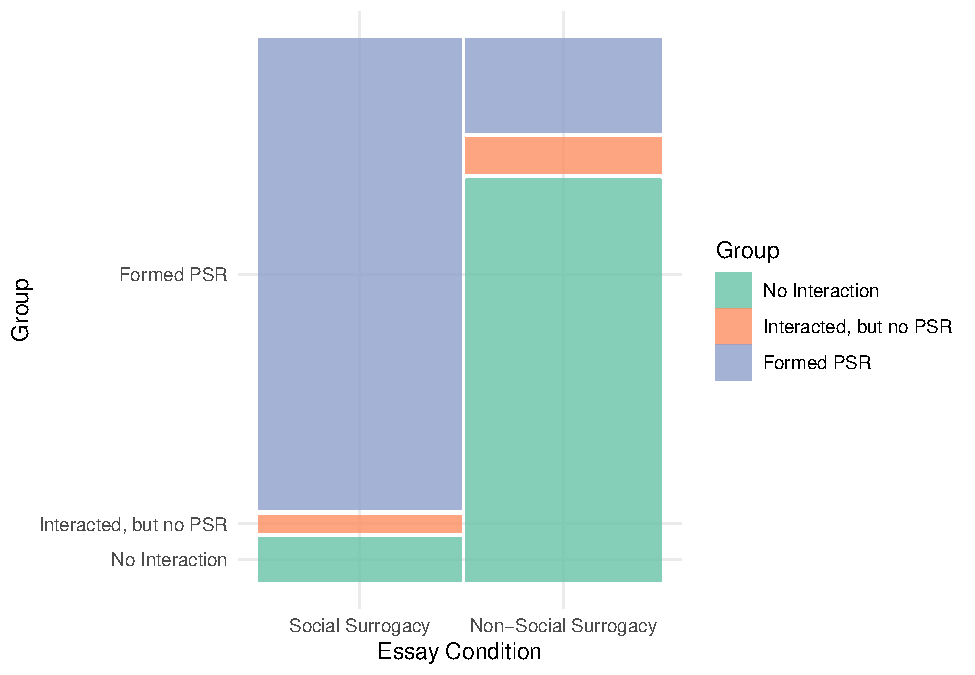
\includegraphics[keepaspectratio]{Sunami-Dissertation_files/figure-latex/exp-mosaic-1.pdf}}
\caption{\label{fig:exp-mosaic}Study 2 - Proportions of Participabts who Reported experiencing Parasocial Relationships with an NPC across Conditions}
\end{figure}

To further probe the effectiveness of the manipulation on inducing parasocial relationships, I used the modified Parasocial Interaction-Process Scale (\citeproc{ref-schrammPSIProcessScalesNew2008}{Schramm \& Hartmann, 2008}). Only participants who indicated that they interacted with an non-player character answered this scale. I ran Welch's \emph{t}-test on the modified Parasocial Interaction-Process Scale to compare the levels of parasocial relationship participants formed in a social surrogacy game vs a non-surrogacy game. Results suggested that participants in the social surrogacy game condition (\emph{M} = 2.32, \emph{SD} = 0.65) reported higher parasocial interaction than those in the non-social surrogacy game condition (\emph{M} = 1.77, \emph{SD} = 0.75, \emph{t}(59.6) = 4.43, \emph{p} \textless{} .001, \emph{d} = 0.82, 95\%CI {[}0.47, 1.16{]}, see Figure \ref{fig:exp-plots}, Panel A).

\begin{figure}
\centering
\pandocbounded{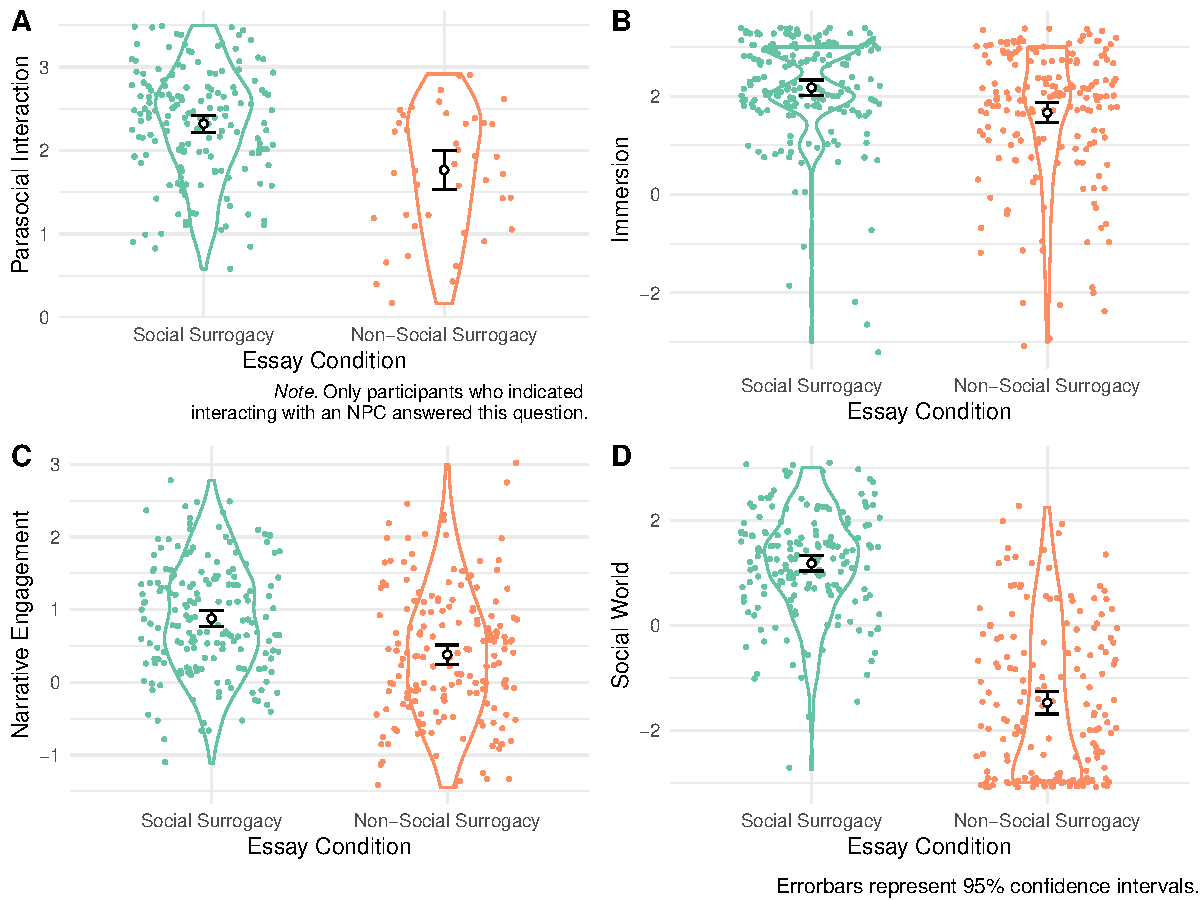
\includegraphics[keepaspectratio]{Sunami-Dissertation_files/figure-latex/exp-plots-1.pdf}}
\caption{\label{fig:exp-plots}Study 2: Exploratory manipulation check items across essay conditions.}
\end{figure}

To explore the effectiveness of the video game essay in inducing social worlds, I ran a Welch's \emph{t}-test to compare the scores of the Single-Item Immersion Scale (\citeproc{ref-reysenInitialValidationReliability2019}{Reysen et al., 2019}), the Narrative Engagement Scale (\citeproc{ref-busselleMeasuringNarrativeEngagement2009}{Busselle \& Bilandzic, 2009}), and the on-the-fly measure of social world, between social surrogate vs.~non-social surrogate video game essay conditions. I expected that rejected participants who wrote about the social surrogacy video game would report higher immersion and social worlds compared with those who wrote about their non-social surrogacy video game. Results were consistent with these predictions. Participants in the social surrogate essay condition reported higher immersion (\emph{M} = 2.17, \emph{SD} = 1.06) than those in the non-social surrogate essay condition (\emph{M} = 1.66, \emph{SD} = 1.36, \emph{t}(330.3) = 3.95, \emph{p} \textless{} .001, Figure \ref{fig:exp-plots}, Panel B). Participants in the social surrogate essay condition reported higher narrative engagement (\emph{M} = 0.88, \emph{SD} = 0.76) than those in the non-surrogacy essay condition (\emph{M} = 0.38, \emph{SD} = 0.90, \emph{t}(342.0) = 5.60, \emph{p} \textless{} .001, Figure \ref{fig:exp-plots}, Panel C). Participants in the social surrogate essay condition reported higher social worlds (\emph{M} = 1.18, \emph{SD} = 1.00) than those in the non-social surrogate essay condition (\emph{M} = -1.47, \emph{SD} = 1.46, \emph{t}(306.0) = 19.99, \emph{p} \textless{} .001, Figure \ref{fig:exp-plots}, Panel D).

Note that the Inclusion of Self in the Other Scale (\citeproc{ref-aronInclusionOtherSelf1992}{Aron et al., 1992}), the Single-Item Immersion Scale (\citeproc{ref-reysenInitialValidationReliability2019}{Reysen et al., 2019}), and the on-the-fly measure of social world have never been validated to measure social surrogates in video games, and thus I treat these analyses as exploratory. In the proposal, I pointed out that a failed manipulation check in this context can be ambiguous---such results can imply that (a) the manipulation was ineffective to induce parasocial relationships and social worlds, or (b) the measures were ineffective to capture the manipulated constructs. Even with the current positive results, I cannot rule out the latter possibility that the measures were ineffective in capturing social surrogates in video games. Accordingly, I do not conclude the effectiveness of the manipulation based on these exploratory analyses.

\textbf{Exploratory Analysis of Enjoyment across Social Surrogacy vs.~Non-Social Surrogacy Games.} To explore whether levels of enjoyment differed for social Surrogacy vs.~non-social Surrogacy video conditions, I performed Welch's \emph{t}-test. I did not have a priori hypothesis for this analysis. Participants in the social surrogate condition (\emph{M} = 2.49, \emph{SD} = 0.57) reported more enjoyment in playing a game in their essay than those in the non-social surrogate condition (\emph{M} = 2.13, \emph{SD} = 0.82, \emph{t}(312.4) = 4.75, \emph{p} \textless{} .001, Figure \ref{fig:enjoyment-plot}).

\begin{figure}
\centering
\pandocbounded{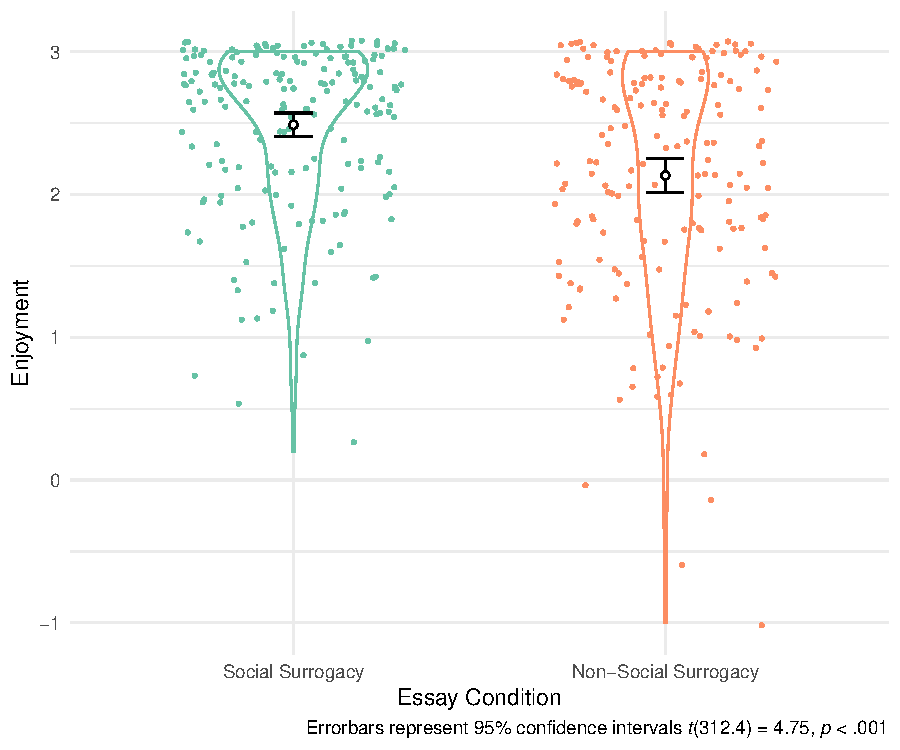
\includegraphics[keepaspectratio]{Sunami-Dissertation_files/figure-latex/enjoyment-plot-1.pdf}}
\caption{\label{fig:enjoyment-plot}Study 2 - Enjoyment across Essay Conditions}
\end{figure}

\subsection{Unplanned Analyses}\label{unplanned-analyses}

Below I report analyses that I did not plan in the proposal of this dissertation.

\textbf{Self-Assessment Manikin Scores by Conditions and Time}. To probe whether participants experienced different arousal, valence, dominance, after writing a social surrogate vs.~non-surrogate essay, I ran 2 (Essay Condition: Social Surrogacy vs.~Non-Social Surrogacy) x 2 (Time: Time 1 vs.~Time 2) Mixed ANOVAs on the Self-Assessment Manikin Scores. For the Heart Manikin scores, there was no main effect of the Essay (\emph{F}(1,420) = 0.03, \emph{p} = .869, \(\eta^2_{G}\) \textless{} .001), no main effect of Time (\emph{F}(1,420) = 1.24, \emph{p} = .265, \(\eta^2_{G}\) \textless{} .001), and no Essay Type x Time interaction interaction (\emph{F}(1,420) = 0.33, \emph{p} = .568, \(\eta^2_{G}\) \textless{} .001). For the original Self-Assessment Manikins (Valence, Arousal, and Dominance), there were no main effect of the Essay type (\emph{F}(1,420) = 0.07, \emph{p} = .791, \(\eta^2_{G}\) \textless{} .001 for valence, \emph{F}(1,419) = 0.56, \emph{p} = .453, \(\eta^2_{G}\) \textless{} .001 for arousal, and \emph{F}(1,420) = 0.10, \emph{p} = .752, \(\eta^2_{G}\) \textless{} .001 for dominance) or no Essay x Time interaction (\emph{F}(1,420) = 6.47, \emph{p} = .011, \(\eta^2_{G}\) = .002 for valence, \emph{F}(1,419) = 1.99, \emph{p} = .159, \(\eta^2_{G}\) \textless{} .001 for arousal, and \emph{F}(1,420) = 0.01, \emph{p} = .920, \(\eta^2_{G}\) \textless{} .001 for dominance). However, there were main effects of Time across these measures (\emph{F}(1,420) = 17.86, \emph{p} \textless{} .001, \(\eta^2_{G}\) = .006 for valence, \emph{F}(1,419) = 74.78, \emph{p} \textless{} .001, \(\eta^2_{G}\) = .035 for arousal, and \emph{F}(1,420) = 27.05, \emph{p} \textless{} .001, \(\eta^2_{G}\) = .005 for dominance), suggesting that participants reported higher valence, arousal, and dominance at Time 2 than Time 1.

\begin{figure}
\centering
\pandocbounded{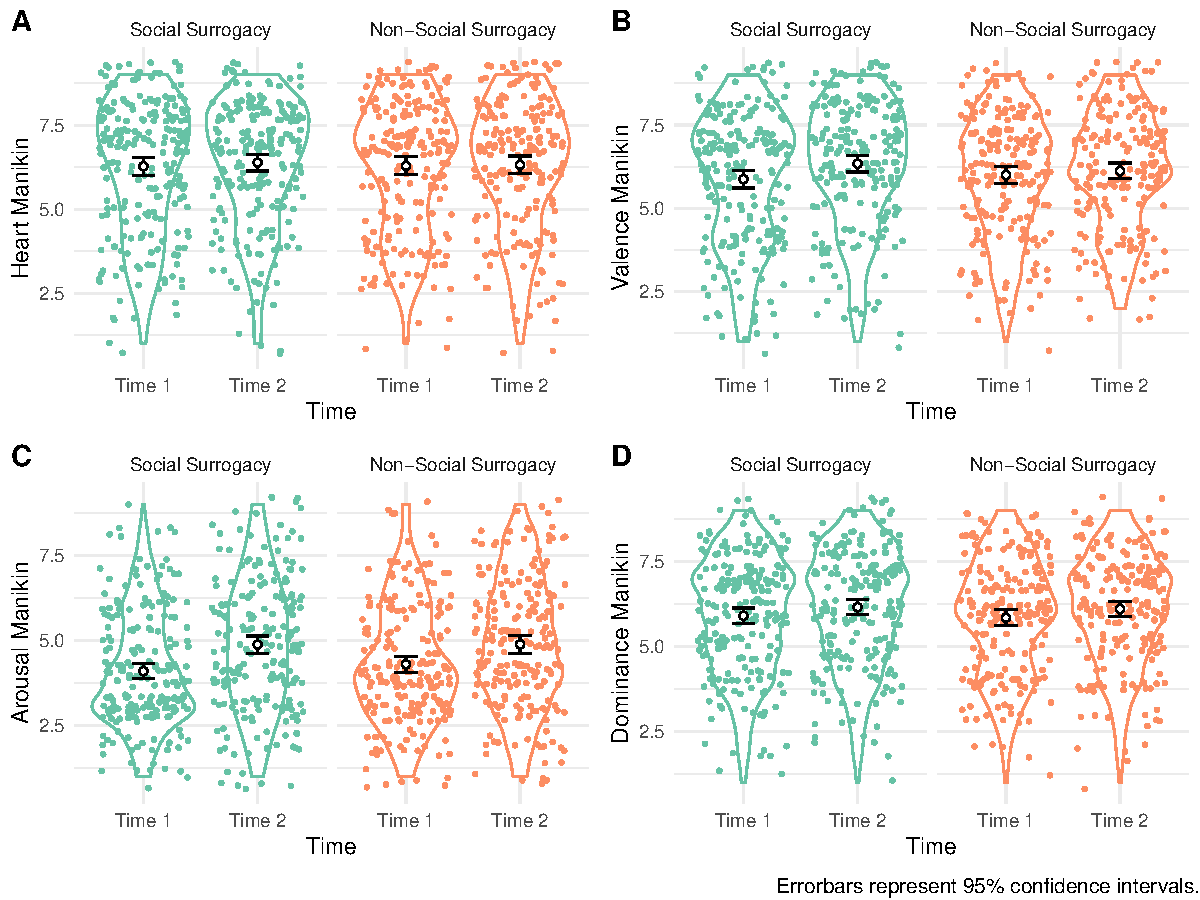
\includegraphics[keepaspectratio]{Sunami-Dissertation_files/figure-latex/manikin12-plot-1.pdf}}
\caption{\label{fig:manikin12-plot}Study 2 - Manikin Scores Across Conditions}
\end{figure}

\textbf{Moderation by Indicators of Parasocial Relationships, Social World, and Enjoyment}. I explored whether measures of parasocial relationship, social world, or enjoyment moderated the effects of the social surrogacy essay manipulation on Heart Manikin in a series of mixed models. I constructed a mixed model for each moderator variable (the manipulation check groups {[}Groups 1-3{]}, Inclusion of the Other in Self Scale, Parasocial Interaction-Process Scale, Narrative Engagement, Single-Immersion Scale, and the On-The-Fly Measure of Social World, and enjoyment). Thus, each model contained the following fixed predictors: the moderator, the essay condition (Essay: social surrogacy vs.~non-social surrogacy), Time (Time 1 vs.~Time 2), the 2-way Moderator x Essay interaction, the 2-way Moderator x Time interaction, the 2-way Essay x Time interaction, and the 3-way Moderator x Essay x Time interaction. All categorical predictors were sum contrast-coded (effect-coded), and all continuous predictors were centered to the grand mean. Below, I only report positive results for the purpose of brevity. The full results are available in {[}Appendix{]}. Note that these results were not preregistered and thus prone to Type I error.

For the model with the Inclusion of the Other in Self scores as a moderator, there was a two-way interaction between the Inclusion of the Other in Self scores and Time (\emph{B} = -0.08, \emph{SE} = 0.03, \emph{t} = -2.44, \emph{p} = .015; Figure \ref{fig:s2-mod-plot}, Panel A). However, follow-up tests showed that the relationship between the Inclusion of the Other in Self scores and the Heart Manikin scores were not different from zero at both Times 1 and 2.

\begin{figure}
\centering
\pandocbounded{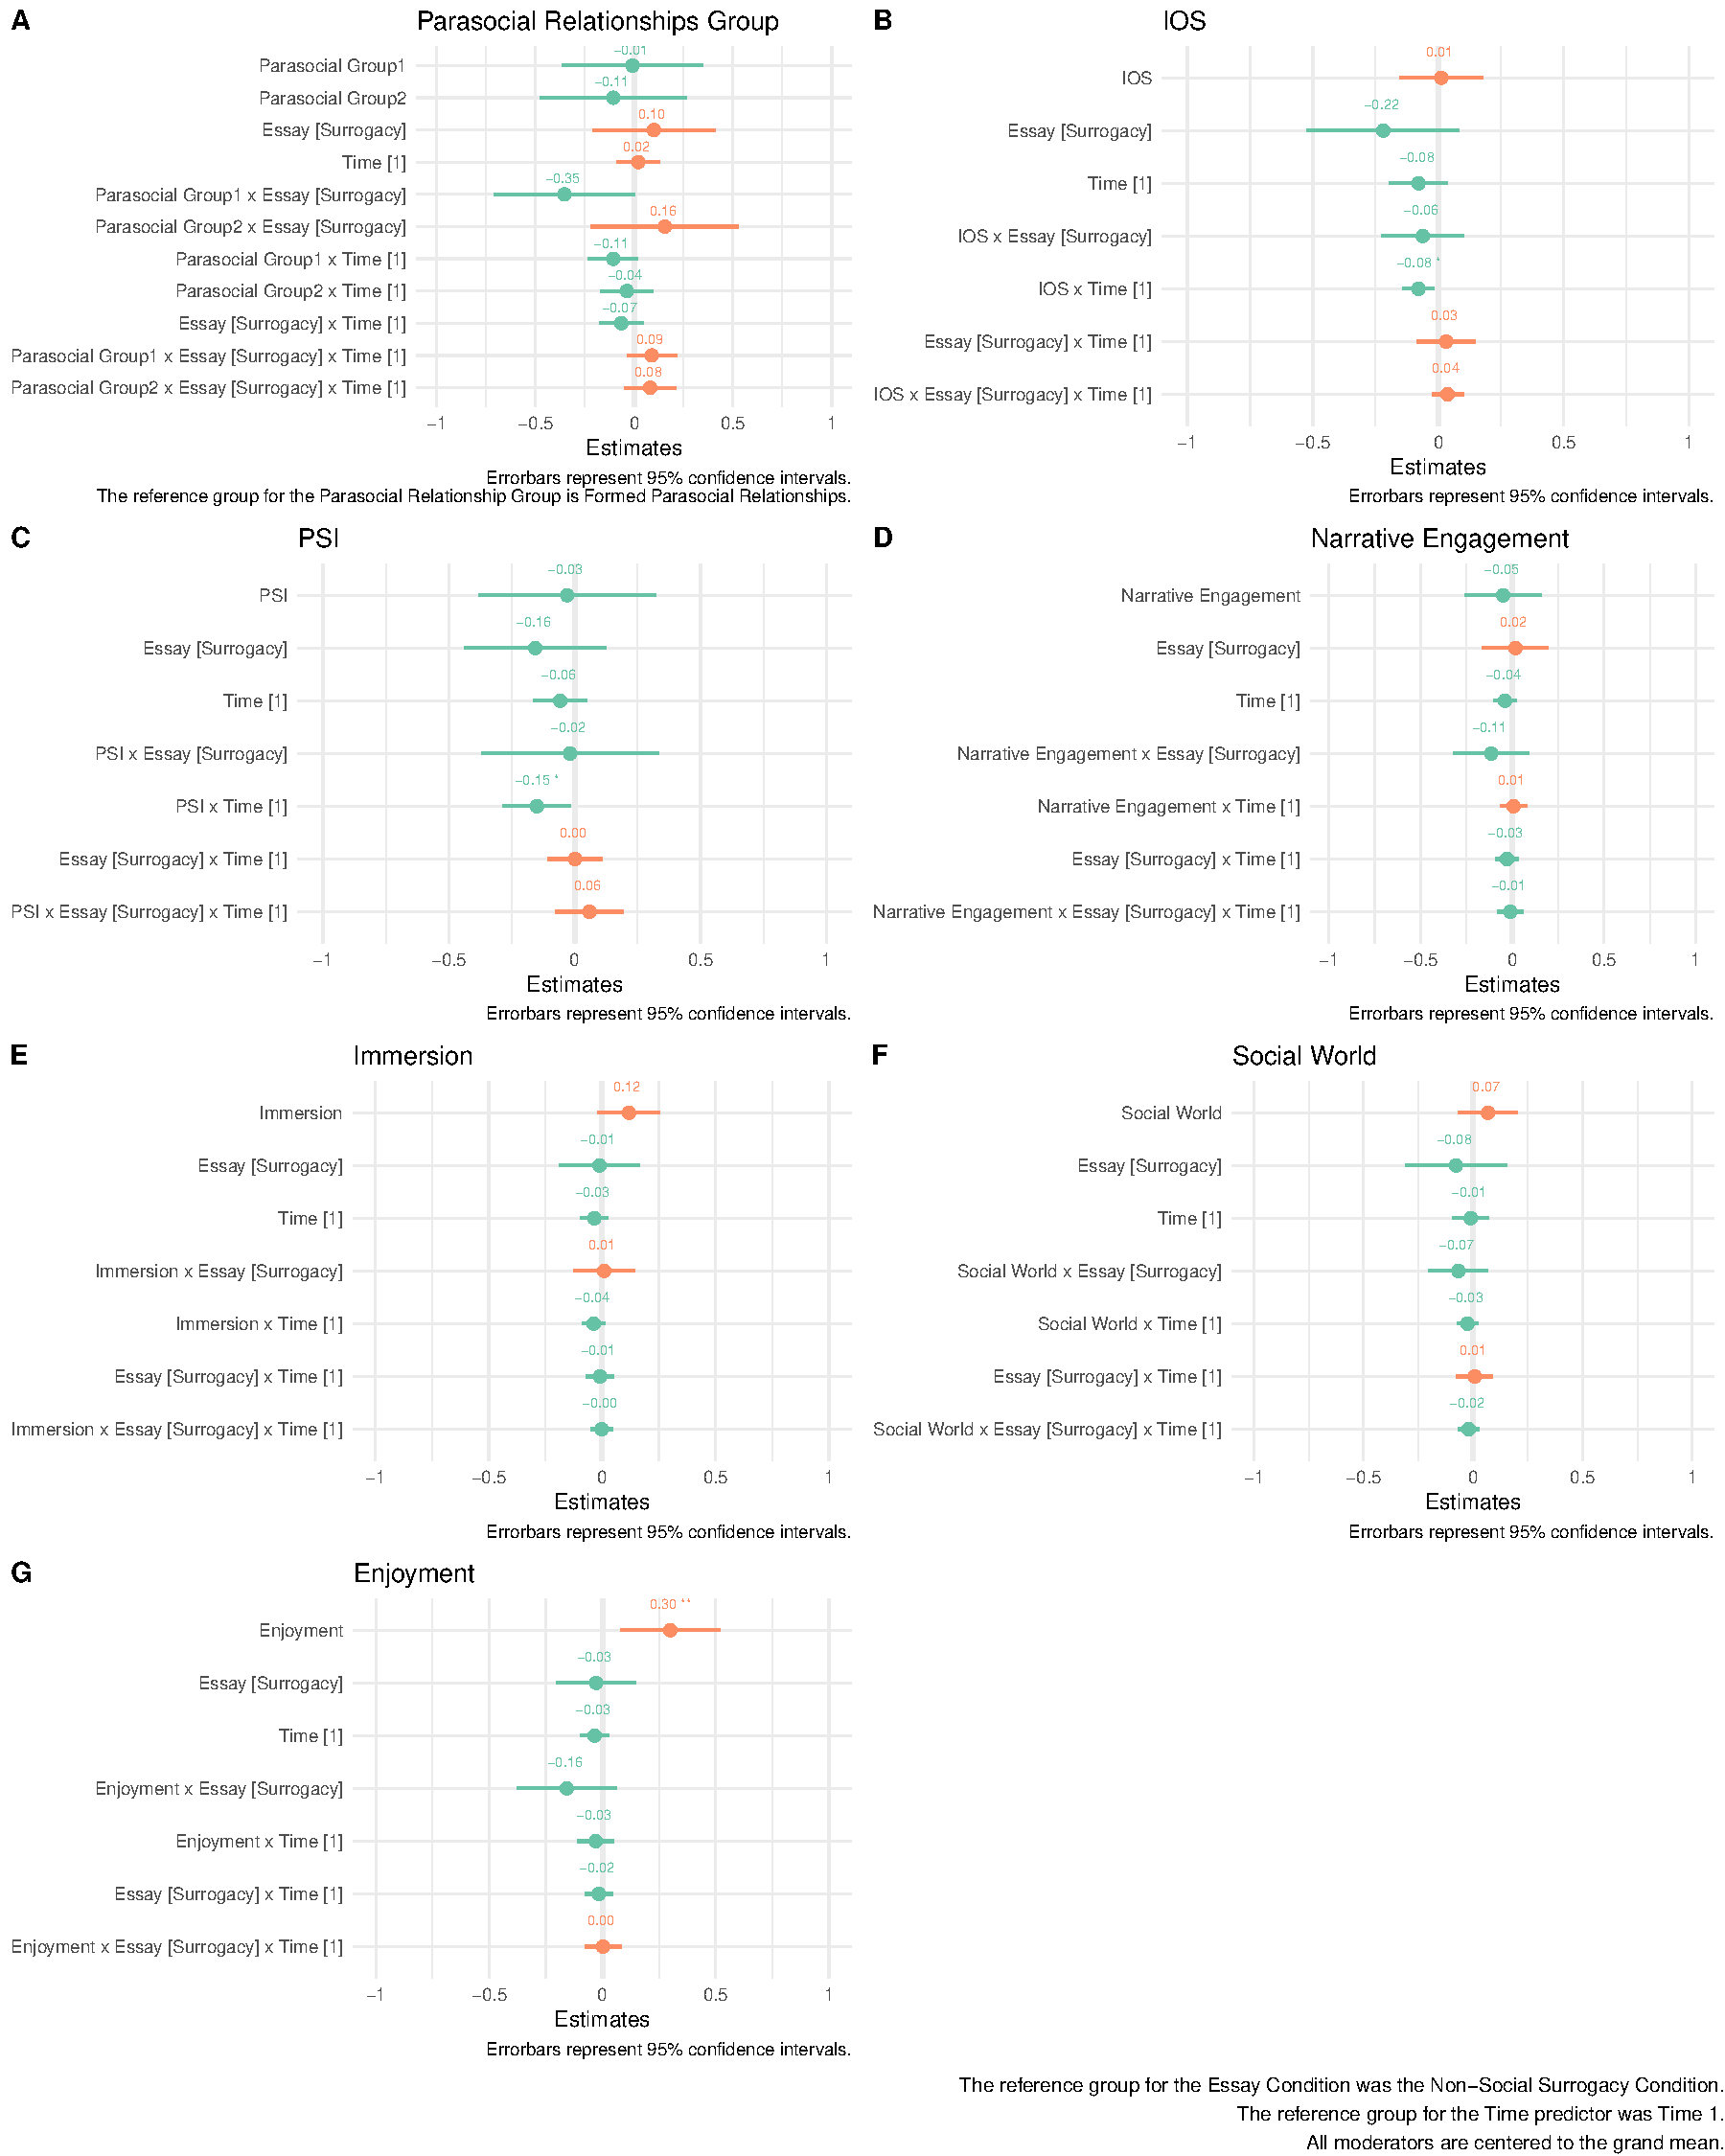
\includegraphics[keepaspectratio]{Sunami-Dissertation_files/figure-latex/s2-mod-plot-1.pdf}}
\caption{\label{fig:s2-mod-plot}Study 2 - Probing Parasocial Relationships, Social World, and Enjoyemnet as Moderators Predicting Heart Manikin Scores}
\end{figure}

Similarly, for the model testing the Parasocial Interaction scores as a moderator, there was a two-way interaction between the Parasocial Interaction scores and Time (\emph{B} = -0.15, \emph{SE} = 0.07, \emph{t} = -2.17, \emph{p} = .031; Figure \ref{fig:s2-mod-plot}, Panel C). However, follow-up tests showed that the relationship between the Parasocial Interaction scores and the Heart Manikin scores were not different from zero at both Times 1 and 2.

For the model with the with Enjoyment with the moderator, participants reporting higher enjoyment reported higher Heart Manikin scores than those with lower enjoyment, regardless of the essay condition or time (\emph{B} = 0.30, \emph{SE} = 0.11, \emph{t} = 2.65, \emph{p} = .008; Figure \ref{fig:s2-mod-plot}, Panel G). These results suggest that participants who enjoyed the game in their essay reported more belonging across the study.

\textbf{Bivariate Correlation Analysis}. I explored associations among the measured variables in this study in a bivariate correlation analysis. I only report select positive associations here. For the full correlation matrix, see Table \ref{tab:s2-correlations-table} in {[}Appendix{]}. Note that these analyses were not planned a priori, and prone to Type I error. Participants with higher Heart Manikin at Time 2 reported higher immersion and enjoyment, compared with those with lower Heart Manikin scores. Measures of parasocial relationship, social world, and enjoyment are positively correlated with each other. For example, participants who felt closer to a non-player character were more immersed, more engaged in the story, and experiencing more social world.

\section{Discussion}\label{discussion-1}

Based on Hypothesis 1, I expected that participants in the social surrogacy game condition report more belonging than those in the non-social surrogacy game condition. The current results did not confirm this hypothesis. Instead, the people who wrote about the social surrogacy video game reported similar levels of belonging compared with the people who wrote about non-social surrogacy game. The difference was theoretically equivalence to zero according the equivalence test. The reasons for the current null results include: (a) Type II error, (b) ineffective social rejection induction or essay manipulations, (c) failure of the social rejection induction or the social surrogacy manipulation, (d) passage of time after rejection recovering belonging, (e) confusion in nominating video games, and (f) non-surrogacy video games providing belonging.

\textbf{Type II Error: Failure to Detect a True Effect by Chance}. We can attribute the current results to a Type II error, failing to observe a true effect by chance. I reduced the likelihood of the Type II error for the study by setting the power to .90 in the a priori power analysis. That being said, I assumed that the true effect was at least \emph{d} = 0.35. A possibility remains that the true effect size was smaller than \emph{d} = 0.35, and thus the current study was not effective for detecting the effect.

\textbf{Failure of Inducing Social Rejection, or Manipulating Social Surrogacy}. I also can attribute the current results to the ineffective induction of social rejection or the ineffective manipulation of social surrogacy. Participants may have not felt rejected by the rejection induction, or participants did not experience social surrogacy in the social surrogacy essays. However, I suggest that these possibilities are unlikely for the following reasons. First, the social rejection induction in this study was found highly effective in Study 1c (ARv1), using the same Heart Manikin Measure (\emph{d} = -2.12, 95\%CI {[}-2.41, -1.83{]}). Second, participants who wrote a social surrogacy essay reported more parasocial relationships, immersion, engagement with narrative, social world, and enjoyment than those who wrote a non-social surrogacy essay. Although I do not conclude about the effectiveness of the manipulations as planned, these results add to the confidence that the manipulations were relevant to social surrogacy. Overall, I am skeptical of a possibility that the social rejection induction or the social surrogacy manipulation failed in this study.

\textbf{Time After Rejection Simply Recovering Belonging}. Participants may have recovered their belonging simply because of the passage of time from the rejection essay. Past research has shown that participants ostracized in Cyberball (an online ball-tossing game) showed recovery towards positive affect after about 2 minutes (\citeproc{ref-wesselmann2012}{Wesselmann et al., 2012}). In Study 1c (ARv1) and Study 1d (EVv1), rejected participants recovered belonging after socially rejected (see Figures \ref{fig:s1c-sensitivity-plot} and \ref{fig:s1d-sensitivity-plot}). Thus, in the same manner, the participants in this study could have recovered belonging simply after the 3-minute essay, regardless of the content of the essay.

\textbf{Confusion in Nominating Video Games}. Participants may have had a difficulty in following the instructions to nominate social surrogacy and non-social surrogacy games, and they might not be able to nominate correct type of games. I avoided this possibility in 2 ways, First, I provided descriptions and examples of social- and non-social surrogacy games in the instructions. Second, I excluded any participants that were deemed as not following the instructions in the exclusion coding procedure. Still, I cannot completely rule out this possibility because 12.14\% of participants failed to follow the instructions as per the exclusion procedure, adding to a possibility that participants may have had a hard time understanding the instructions. I repeated the main analysis with the excluded participants and found results consistent with the sample with exclusions (see \hyperref[main-analysis-with-excluded-participants]{Appendix}).

\textbf{Non-Social Surrogacy Video Games Providing Belonging}. Another possible reason for the null results is that writing about non-social surrogacy games provided belonging. The social surrogacy hypothesis suggests that people can replenish belonging via a reminder of others---non-human entities that reminds of social connections such as pictures of friends, comfort food, and Facebook updates (\citeproc{ref-gabrielSocialSurrogatesRejection2017}{Gabriel \& Valenti, 2017}). The non-social surrogacy games in the current study could have served as reminders of others in a similar manner. For example, people who played Tetris with their close friends can remember their social connections while thinking about Tetris, and thus replenishing belonging. In Study 3, I eliminated this possibility by asking participants play a novel video game that they have never played before.

Overall, the current results did not support the social surrogacy hypothesis--I did not find evidence that people can replenish belonging via social surrogates in video games. Rejected participants reported similar levels of belonging regardless of writing a social surrogacy or non-surrogacy essay. The current results do not offer a clear answer to why all participants recovered belonging. As mentioned above, the current study had methodological limitations. In Study 3, I continued testing the social surrogacy hypothesis by a novel video game that directly manipulates social surrogates. This at minimum addressed the possible issues of unclear instructions and previous experience to a video game.

\chapter{Study 3: Can Playing a Single-Player Video Game Replenish Belonging via Parasocial Relationships and Social Worlds?}\label{study-3-can-playing-a-single-player-video-game-replenish-belonging-via-parasocial-relationships-and-social-worlds}

Study 2 tested whether recalling about a time playing a social surrogacy
video game can replenish belonging after social rejection. Social
surrogate video games involve two distinct social surrogates, according
to the social surrogacy hypothesis. First, people who write about a
social surrogacy video game may experience parasocial
relationships---they may have thought about emotional bonds with their
favorite characters like players of the Mass Effect series report
attachments to Tali and Garrus (\citeproc{ref-burgess2020a}{Burgess \& Jones, 2020}). Second, people may have
experienced social worlds---they may have remembered the time they were
immersed in the story and felt like being a member of the game's social
world. Although Study 2 tested that social surrogates could replenish
belonging following social rejection, whether parasocial relationships,
social worlds, or the combination of the two can increase belonging in
single-player games remains unknown.

In Study 3, I decomposed the effects of parasocial relationships and the
social world on belonging after social rejection. To do so, I developed
an original game to independently manipulate the degree of parasocial
relationships (high vs.~low) and social worlds (high vs.~low). Using a
new original video game also eliminated any influence from participants'
familiarity with the game since all participants played this game for
the first time. All participants first experienced social rejection and
then played the video game with varying degrees of parasocial
relationships and social worlds. The goal of this study was to test
Hypotheses 2, 3, and 4.

I label degrees of parasocial relationships and social worlds as high
vs.~low, instead of present vs.~absent, since people see social agency
in most visual stimuli even in geometric figures
(\citeproc{ref-heiderExperimentalStudyApparent1944}{Heider \& Simmel, 1944}; \citeproc{ref-schollPerceptualCausalityAnimacy2000}{Scholl \& Tremoulet, 2000}), and thus I cannot rule out the
possibility that people do not experience parasocial relationships or
social worlds.

\section{Method}\label{method-1}

\subsection{Sample Size Rationale}\label{sample-size-rationale-1}

No estimate for the effect size for this study is available, and thus I
used the safeguarded effect size in Study 2 as the target effect size
(\emph{d} = 0.35). The current study was a 2 (Parasocial Relationships: High
vs.~Low) x 2 (Social Worlds: High vs.~Low) between-subjects design. I
followed a recommendation to base the patterns of group mean differences
to estimate an effect size
(\citeproc{ref-lakensSimulationBasedPowerAnalysisFactorial2019}{Lakens \& Caldwell, 2019}). For the current
power analysis, I treated Cohen's \emph{d} as the differences in the group
means by assuming the pooled standard deviation of 1. I used the
\emph{Superpower} R package to perform power analysis
(\citeproc{ref-lakensSimulationBasedPowerAnalysisFactorial2019}{Lakens \& Caldwell, 2019}).

Since the main goal of the study was to test the effects of parasocial
relationships and social worlds on belonging, I calculated the required
sample size based on the main effect of each. I assumed that the main
effects of the parasocial relationship manipulation and the social world
manipulation would each have an effect size of \emph{d} = 0.35 (Hypotheses 2
and 3). The resulting target sample size to achieve .90 power and .05
alpha is 344 participants in total (86 per condition x 4 conditions).
This sample size is enough to detect \emph{d} = 0.50 with .90 power and .05
alpha for the ancillary Hypothesis 4 (86 per group). See Figure
\ref{fig:s3-expected-means} for the expected pattern of the means used
for the power analysis.

\begin{figure}
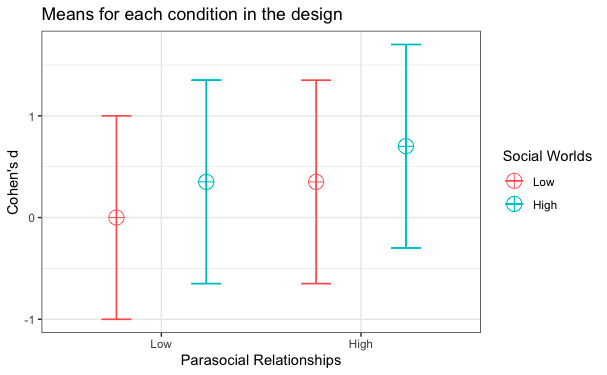
\includegraphics[width=0.7\linewidth]{images/s3-expected-means} \caption{Expected Patterns of the Means Used for the Power Analysis for Study 3}\label{fig:s3-expected-means}
\end{figure}

\emph{Note.} All Cohen's d's are relative to the low parasocial relationship
and the low social world condition (depicted as zero). The error bars
represent +/-1 SD from the estimate.

\subsection{Participants}\label{participants-6}

I recruited 469 participants via the
psychology participant pool at the University of Delaware. The final
analytic sample size was 344 after exclusions
(see Exclusions and Stopping Rule below). Among the included
participants, 207 (60.17\%)
identified as woman, 130 (37.79\%)
identified as man, and 7 (37.79)
identified as neither man or woman. For the racial identity,
265 (77.03\%) identified as White,
39 (11.34\%) as Asian,
15
(4.36\%) as Black/African-American,
and 25
(7.27\%) as belonging to other racial
category or to multiple racial categories. Participants received partial
course credit for participation. Participants were eligible to
participate if they have access to a computer to play the custom game on
a web browser.

The current study used a novel RPG with a fictional story with dialogues
with non-player characters---both important components for the
parasocial relationship and social world manipulations. However, some
people may dislike stories and dialogues and ignore them in their
gameplay. If I recruited only participants disinterested in stories, the
manipulations in this study would be ineffective simply because they are
not paying attention to the manipulation. To minimize the issue, I asked
prospective participants to answer the story subscale of the Gaming
Attitudes, Motives, and Experiences Scale to measure people's interests
in stories in video games (\citeproc{ref-hilgardIndividualDifferencesMotives2013}{Hilgard et al., 2013}).
Then, I prioritized inviting participants with higher interests in
stories for participation.

Prioritizing the participation of people who liked storytelling also
increased the external validity of the study. In reality, single-player
video games with social surrogates are usually role-playing games with
stories and dialogues with other characters. People who regularly play
these games should have interests in stories in the first place since
people usually purchase and play video games they like. If I happen to
only recruit participants who dislike stories, our sample would not be
representative of the consumers of single-player video games with social
surrogates. The results of the study has the most implications for those
who are likely to play single-player video games--prioritizing their
participation incrased the generality and impact of the study in the
long run.

\subsection{Procedure}\label{procedure-1}

Participants accessed an online study website, signed an informed
consent, and completed the demographics questions. Participants also
completed the baseline Heart Manikin (Time 1) and the original
Self-Assessment Manikin, consistent with Study 2. To increase
participants' engagement with the study materials, I offered monetary
incentives for attending to study materials. Specifically, participants
were told that they would complete a pop quiz about the materials of the
study at the end, and if they answered all questions right they would be
entered into a drawing to receive a \$10 Amazon Gift card. Then, all
participants completed the social rejection essay used in Study 2.

After completing the social rejection essay, participants played a
custom single-player video game, called \emph{Shadows of Gaki} (Figure
\ref{fig:s3-screenshots}), developed for this study on RPG Maker MV
(\citeproc{ref-kadokawacorporationRPGMakerMV2015}{KADOKAWA Corporation, 2015}). I programmed the video game to
independently manipulate parasocial relationships and social worlds.
Participants spent on the average of 30.48
minutes to play the game (\emph{M} = 30.48, \emph{SD} = 63.69).

\begin{figure}
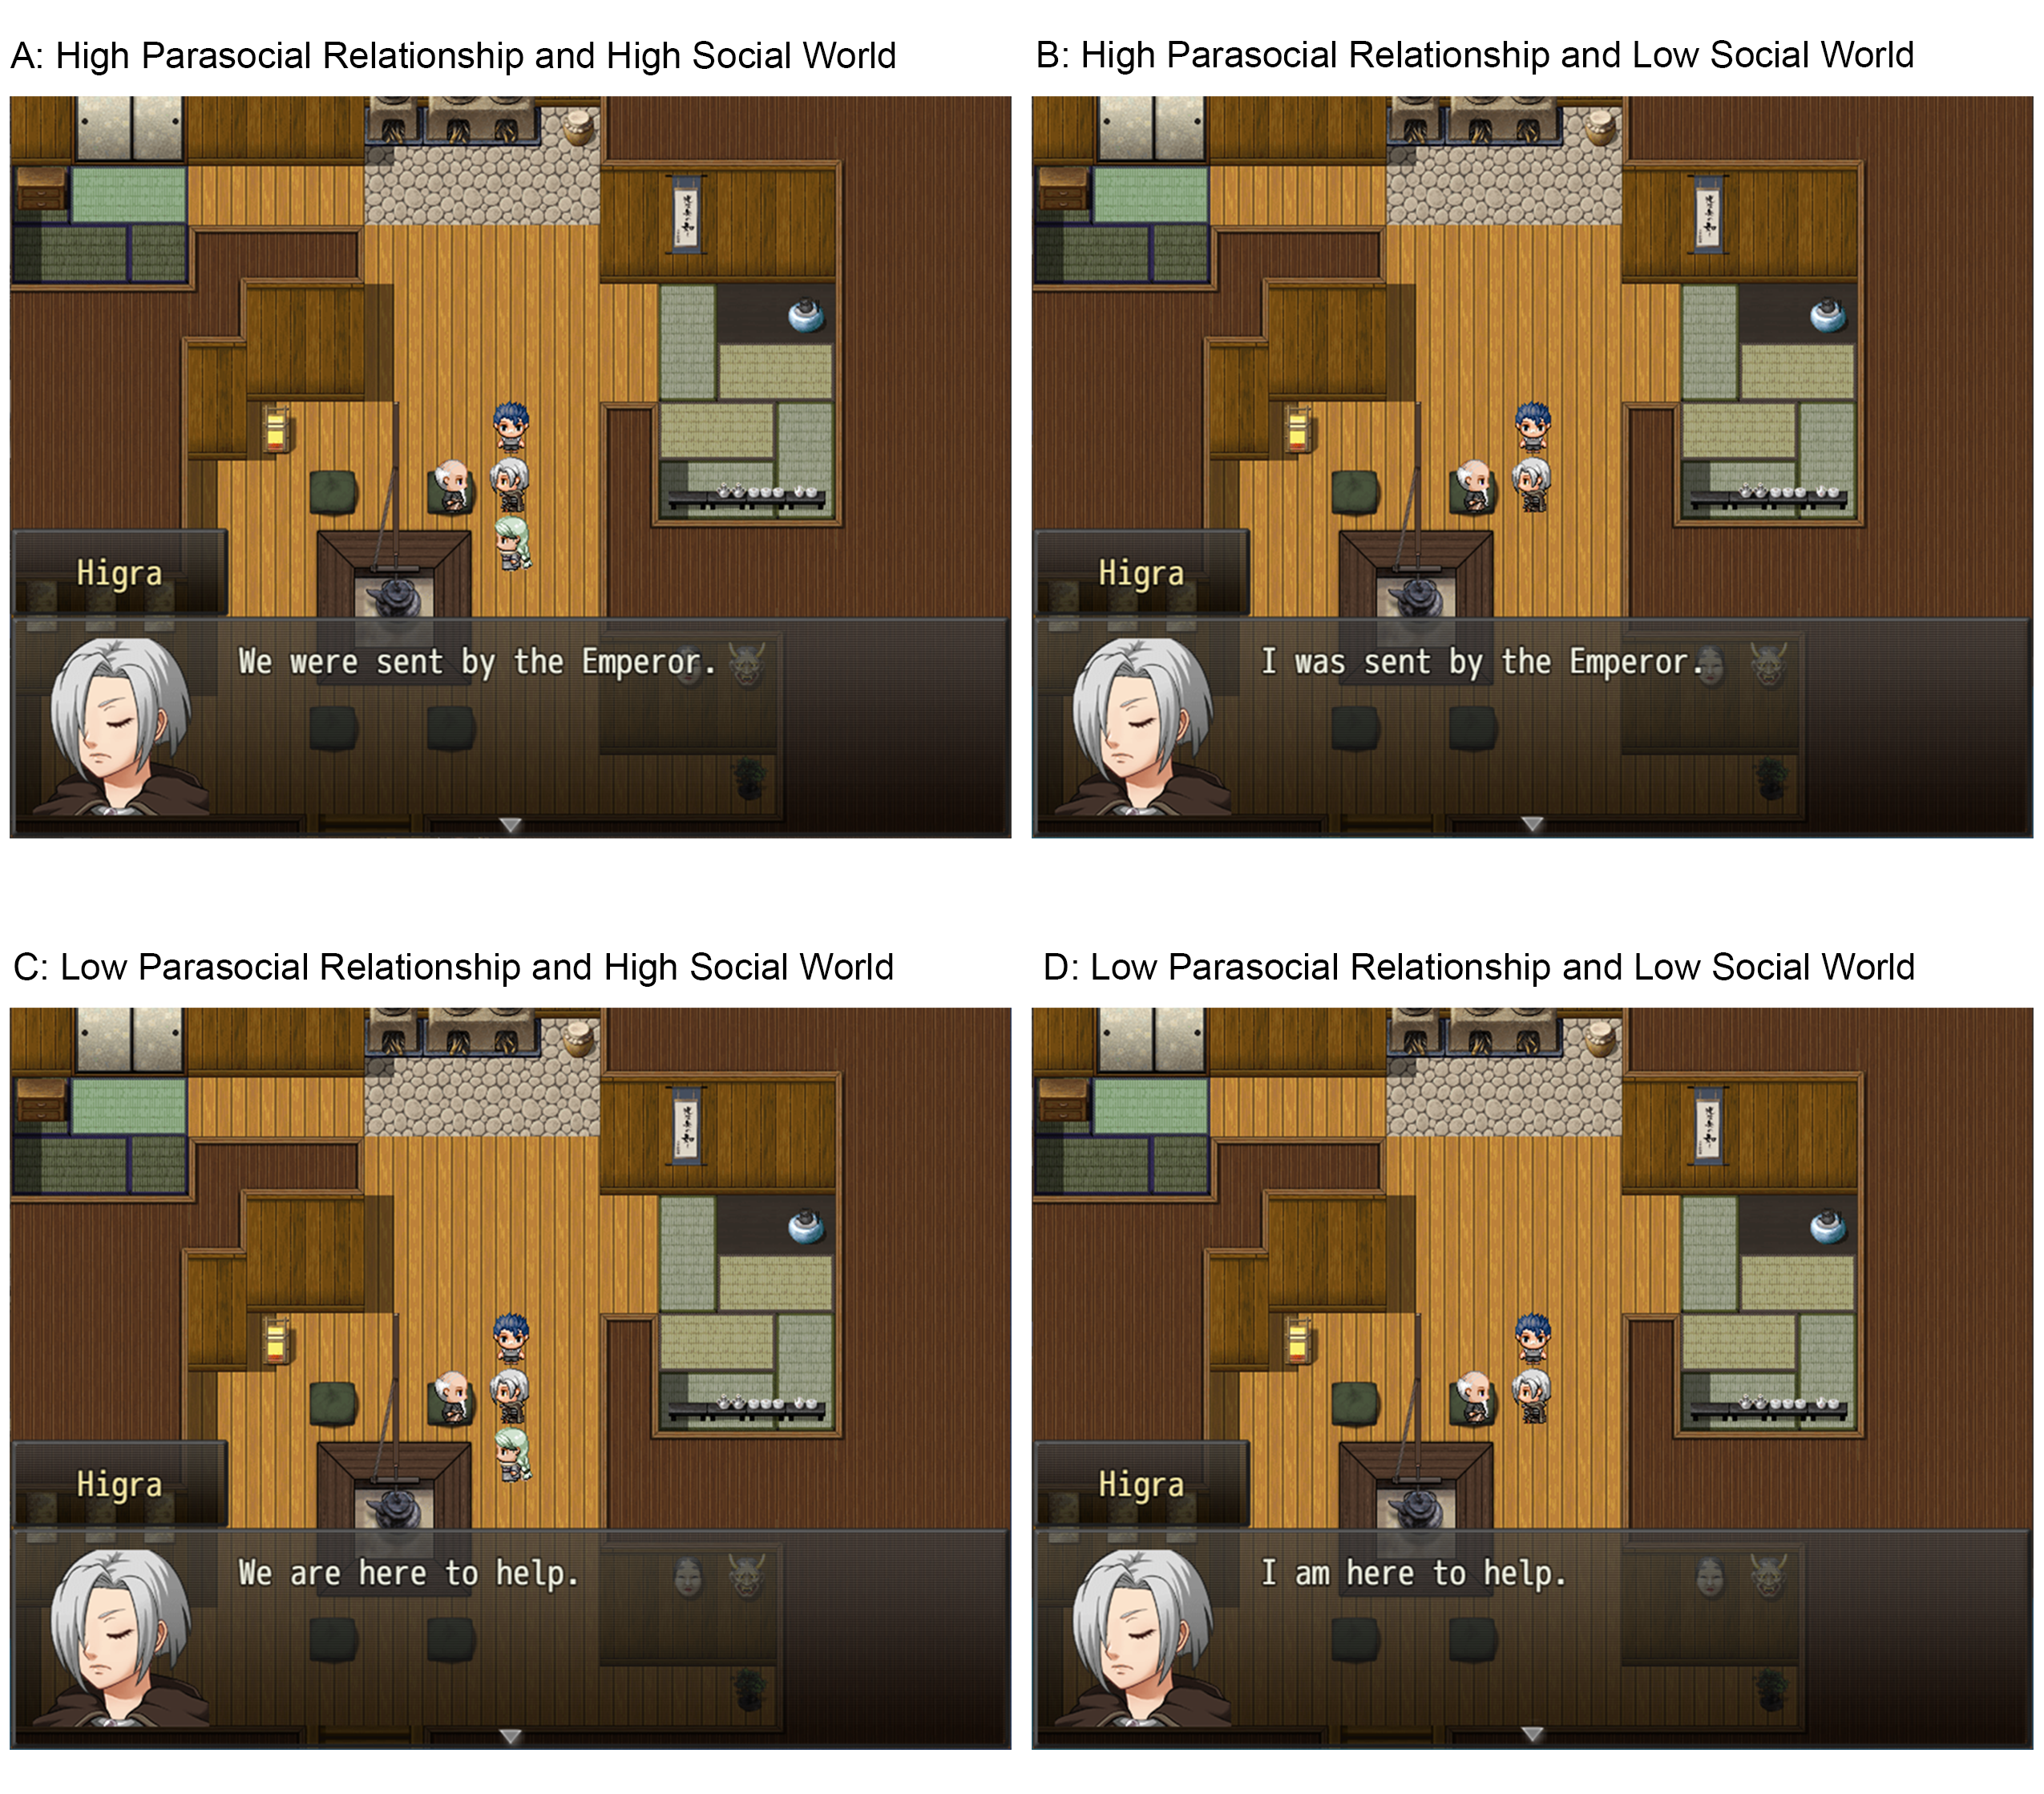
\includegraphics[width=0.9\linewidth]{images/sog-screenshots} \caption{Screenshots from the Custom Video Game, Shadows of Gaki. In the high parasocial relationship conditions (Panels A and B), participants saw a non-player character (Sashu) who followed the player throughout the gameplay. In the low parasocial relationship conditions (Panels B and D), the non-player character was absent. In the high social world conditions (Panels A and B), participants learned about the story that Higra answered the Emperor's call to be a Samga and to reunite with Mother. In the low social world condition, participants will not learn about the story.}\label{fig:s3-screenshots}
\end{figure}

In this game, the player took the role of Higra, the main character who
solves the mystery of a plague affecting the village of Azmar. I set the
gender of the main player character as female for two reasons. First,
past research showed that players adapt the characteristics of the
player character and change how they play the game accordingly (called
the Proteus effect)---such as killing more when playing a male
character, and healing more when playing a female character
(\citeproc{ref-yeeMenHealMore2011}{Yee et al., 2011}). I held the gender of the player character
constant in my game to avoid any influence from the Proteus effect.
Second, women tend to prefer a female character over a male character
whereas men do not have preferences (\citeproc{ref-paikPlayfulGenderSwapping2013}{Paik \& Shi, 2013}; \citeproc{ref-ratanWomenKeepIt2019}{Ratan et al., 2019}). Thus, both female and male participants would
like playing a female player character. For these reasons, I held the
gender of the player character female for all participants.

The contents presented in this single-player game varied depending on
the experimental conditions. I manipulated the parasocial relationships
via the presence of the companion non-player character Sashu. In the
high parasocial relationship condition, the player had an opportunity to
form a parasocial relationship with Sashu. Sashu guided the player
throughout the gameplay and healed the player during the battles if the
player's hit point was low. In the low parasocial relationship
condition, Sashu was not present in the gameplay.

I manipulated the social worlds via the opportunities for immersing into
the story of the video game, and thus facilitating the collective
assimilation (\citeproc{ref-gabrielSocialSurrogatesRejection2017}{Gabriel \& Valenti, 2017}; \citeproc{ref-gabrielBecomingVampireBeing2011}{Gabriel \& Young, 2011}). In the high social world
condition, the player was presented the story of Higra answering the
Emperor's call to be a Samga in the hopes of reuniting with Mother. In
the low social world condition, the player was not presented with these
storytelling components. After playing the video game, participants
completed the Heart Manikin and the original Self-Assessment Manikin
again (Time 2). Then, participants indicated whether they interacted
with the non-player characters in their essay (Yes or No). If the answer
was Yes, they first named the character that they felt most connected to
(``Thinking about the non-player characters {[}NPCs{]} that you interacted
with, whom did you feel most connected to?''), and they completed the
modified Inclusion of Self in Other Scale (\citeproc{ref-aronInclusionOtherSelf1992}{Aron et al., 1992}).
Then, participants completed the modified Single-Item Immersion Scale
(\citeproc{ref-reysenInitialValidationReliability2019}{Reysen et al., 2019}). Then, participants will
complete the modified Single-Item Immersion Scale
(\citeproc{ref-reysenInitialValidationReliability2019}{Reysen et al., 2019}), the on-the-fly measure of
social world, and the Enjoyment Subscale of the Game User Experience
Satisfaction Scale {[}GUESS; Phan et al. (\citeproc{ref-phanDevelopmentValidationGame2016}{2016}){]}. Lastly,
participants completed the identification subscale of the player
character identification scale (\citeproc{ref-vanlooyPlayerIdentificationOnline2012}{Van Looy et al., 2012}),
the attention check items, the questions for the raffle items, and the
open-ended debriefing questions.

\subsection{Measures}\label{measures-1}

The Heart Manikin and the modified Inclusion of Ingroup in the Self
Scale for gamer identification
(\citeproc{ref-troppIngroupIdentificationInclusion2016}{Tropp \& Wright, 2016}) were identical to the ones
used in Study 2. I modified the language of the Inclusion of Self In
Other Scale (\citeproc{ref-aronInclusionOtherSelf1992}{Aron et al., 1992}) used in Study 2 to measure
parasocial relationships with the characters of the custom video game.
Similarly, I modified the language of the Single-Item Immersion Scale
(\citeproc{ref-reysenInitialValidationReliability2019}{Reysen et al., 2019}) and the on-the-fly measure of
social worlds to measure the degrees of immersion and social world while
playing the custom video game. I also modified the language of the
Enjoyment Subscale of the Game User Experience Satisfaction Scale to
refer to the game that participants just played (e.g., ``I thought the
game was fun''). Cronbach's alphas for the current sample were
0.92 for the Enjoyment Subscale of the Game User
Experience Satisfaction Scale, and 0.86 for
the on-the-fly measure of social world.

\textbf{Player Character Identification - Similarity Subscale.} I used the
identification similarity subscale from the Player Character
Identification Scale (\citeproc{ref-vanlooyPlayerIdentificationOnline2012}{Van Looy et al., 2012}). The subscale consisted of 6
statements on the similarities between the player and the player
character (e.g., ``My character is like me in many ways''). I modified
the scale so that they refer to the video game in the study (e.g., ``My
character was like me in many ways''). Cronbach's alpha for the current
sample was 0.96. I treated this scale as
exploratory and thus do not pre-register any analyses.

\textbf{Attention Check.} Consistent with Study 2, participants were asked
about the nature of the first essay: ``In today's study, you were asked
to write an essay. What were you asked to write about?'' Participants
could answer this question as ``about a time I felt rejected'', ``about a
time I felt accepted'', and ``about my morning yesterday''. I marked
participants as failing the attention check if they indicate that they
were asked to write about a time they felt accepted or about their
morning yesterday.

For checking participants' attention to the parasocial relationship
manipulation, I asked participants, ``What was the name of the non-player
character who followed you throughout the gameplay?''. The answer choices
were, ``Sashu'', ``Akiko'' (filler), and ``None---I did not have anyone who
followed me throughout the game''. I marked the following participants as
failing the attention check: participants in the higher parasocial
relationship condition who report ``Akiko'' or ``None'', and participants in
the lower parasocial relationship condition who report ``Sashu'' or
``Akiko''. For checking the social world manipulation, I asked
participants, ``What was the story presented in the game?''. Answer
choices were (a) ``Higra answered the emperor's call and became a Samga,
fighting for good, defeating the evil boss and reuniting with her mother
at the end'', (b) ``Higra prepared a special dish for grandma's birthday''
(Filler), (c) ``Higra battled evil bosses throughout the game, eventually
winning, but did not reunite with her mother at the end.''. I marked the
following participants as failing the attention check: participants in
the higher social worlds condition who answered (b) or (c), and
participants in the lower social worlds condition who answer (a) or (b).

\subsection{Exclusion and Stopping Rule}\label{exclusion-and-stopping-rule}

I excluded any participants who fail to complete the entire study
procedure or fail the attention check.
Eighteen participants failed
the essay attention check,
75 participants
failed the parasocial relationships attention check, and
60 participants
failed the social world attention check. In total, I excluded
125 participants for failing one or more of the three
attention checks.
I also excluded one participant
who stopped the study for more than 4 days while playing the game. I
continued recruiting participants until the sample size after exclusions
reached the target sample size.

\subsection{Deviations from the Proposal}\label{deviations-from-the-proposal}

I proposed to use the Parasocial Interaction---Process Scale
(\citeproc{ref-schrammPSIProcessScalesNew2008}{Schramm \& Hartmann, 2008}) and the modified Narrative Engagement
Scale (\citeproc{ref-busselleMeasuringNarrativeEngagement2009}{Busselle \& Bilandzic, 2009}). After testing the
study, I found that the entire study was taking longer than anticipated.
To reduce the time of participation, I decided to remove these two
scales. Then, participants completed the modified Single-Item Immersion
Scale (\citeproc{ref-reysenInitialValidationReliability2019}{Reysen et al., 2019}), the modified Narrative
Engagement Scale (\citeproc{ref-busselleMeasuringNarrativeEngagement2009}{Busselle \& Bilandzic, 2009}), the
on-the-fly measure of social world, and the Enjoyment Subscale of the
Game User Experience Satisfaction Scale {[}GUESS;
Phan et al. (\citeproc{ref-phanDevelopmentValidationGame2016}{2016}){]}.

Initially, the answer choices for the social world were (a) ``Higra
answered the Emperor's call to be a Samga and reunited with Mother'', (b)
``Higra prepared a special dish for grandma's birthday'' (Filler), and (c)
``None---I did not see any story in the video game''. After recruiting
19 participants, I saw that many participants in the lower
social world condition still answered seeing a story (a) rather than
seeing none (c). I speculated that some participants in the lower social
condition may have imagined their own story while playing the game, thus
not choosing (c). To prevent this issue, I changed the answer choices to
(c) ``Higra battled evil bosses throughout the game.'' After recruiting
another 247 participants, I still saw that this issue
persisted. I further changed the answer choices to (a) ``Higra answered
the emperor's call and became a Samga, fighting for good, defeating the
evil boss and reuniting with her mother at the end'' and (c) ``Higra
battled evil bosses throughout the game, eventually winning, but did not
reunite with her mother at the end.''
Two hundred three participants
completed this final version.

\section{Results}\label{results-6}

\textbf{Main Analysis}. I ran a 2 (Parasocial Relationships: High vs.~Low) x
2 (Social Worlds: High vs.~Low) ANOVA on the Heart Manikin scores at
Time 2. Contrary to the predictions, I did not observe the main effect
of the parasocial relationships (Hypothesis 2;
\emph{F}(1, 340) = 0.87, \emph{p} = .353), and the main effect of the social worlds
(Hypothesis 3; \emph{F}(1, 340) = 0.94, \emph{p} = .333). Similarly, I also did not
observe the Parasocial Relationships x Social Worlds interaction effect
(\emph{F}(1, 340) = 0.12, \emph{p} = .726). As a planned contrast, I
compared the belonging scores of those in the Low Parasocial
Relationships and Low Social Worlds condition to those in the High
Parasocial Relationships and High Social Worlds condition to test
Hypothesis 4. Results did not show a difference in Heart Manikin Scores
at Time 2 (\emph{t} = -1.29, \emph{p} = .568, \emph{d} = -0.20, 90\%CI {[}-0.46, 0.06{]}; Figure
\ref{fig:s3-heart2-plot} A).

Since the obtained p-values were greater than .05 for the analyses for
Hypotheses 2, 3, and 4, I performed the two one-sided test of
equivalence, consistent with the procedure in Study 2 (Lakens, 2017).
Again all effect sizes smaller than \textbar{}\emph{d}\textbar{} = 0.35 are
considered theoretically equivalent to zero. The 90\% confidence
intervals fell within the SESOI for the main effect of the parasocial
realationships (\emph{d} = -0.05, 90\%CI {[}-0.20, 0.11{]}) and the main effect
of social world (\emph{d} = -0.09, 90\%CI {[}-0.24, 0.06{]}). The Cohen's d
contrasting the High Parasocial-High Social World and the Low
Parasocial-Low Social World contained the SESOI, and thus the results
were ambiguous (\emph{d} = -0.20, 90\%CI {[}-0.46, 0.06{]}; Figure
\ref{fig:fig:s3-heart2-plot} B). These results suggest that the main
effects of parasocial relationships and social world were theoretically
equivalent to zero.

\begin{figure}
\centering
\pandocbounded{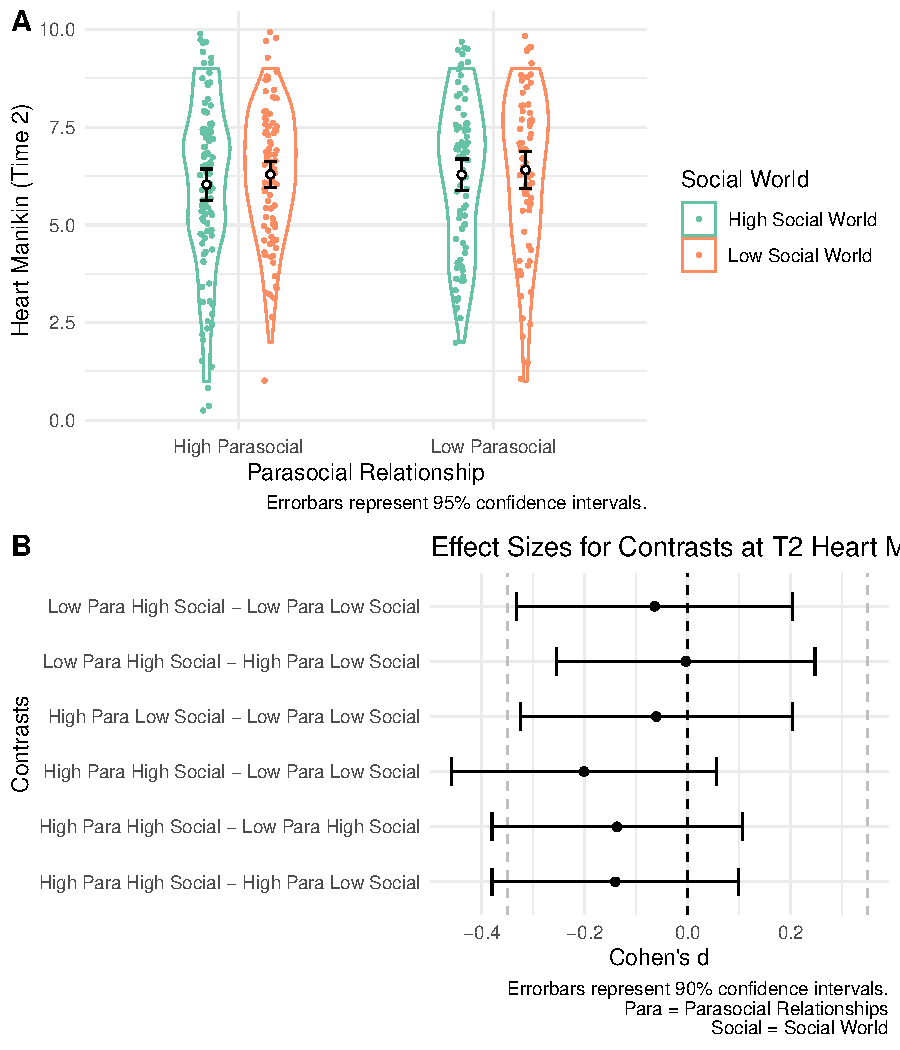
\includegraphics[keepaspectratio]{Sunami-Dissertation_files/figure-latex/s3-heart2-plot-1.pdf}}
\caption{\label{fig:s3-heart2-plot}Study 3 - Heart Mankin Scores at Time 2 Across Parasocial and Social World Conditions}
\end{figure}

\textbf{Exploratory Manipulation Check.} To explore the effectiveness of the
parasocial relationship manipulation, I again used the procedure in
Study 2 to code the participants into three groups: ``did not interact
with non-player characters'' (Group 1), ``interacted with non-player
characters but did not form parasocial relationships'' (Group 2)``, and''interacted with non-player characters and formed parasocial
relationships'' (Group 3). Then, I ran a two-way chi-square test
(Parasocial Relationships: High vs.~Low x Groups: 1, 2, vs.~3) to
examine whether those in the social surrogacy essay condition (vs.~the
non-social surrogacy condition) indicated they interacted with NPCs
(Group 2) and formed parasocial relationships (Group 3) more, rather
than they did not interact with non-player characters (Group 1). Results
did not show any differences in forming parasocial relatioships between
the Higher vs.~Lower Parasocial Relationships conditions
(X2(2, \emph{N} = 344) = 0.71, \emph{p} = .699).

To explore the effectiveness of the social world manipulation, I ran
Welch's \emph{t}-test to compare the scores of the Single-Item Immersion
Scale (Reysen et al., 2019) and the on-the-fly measure of social world
between the High vs.~Low social worlds conditions. Results showed that
participants in the Higher Social World condition reported similar
levels of immersion and social world compared with those in the Lower
Social World condition (for immersion, \emph{t}(331.0) = -0.39, \emph{p} = .700;
for social world measure, \emph{t}(334.4) = 1.30, \emph{p} = .193).

Overall the results of the exploratory manipulation check suggested that
the manipulations may not have affected the target constructs. As
planned, I treat the analyses as exploratory, and do not conclude the
effectiveness of the manipulation based on these analysis.

\begin{figure}
\centering
\pandocbounded{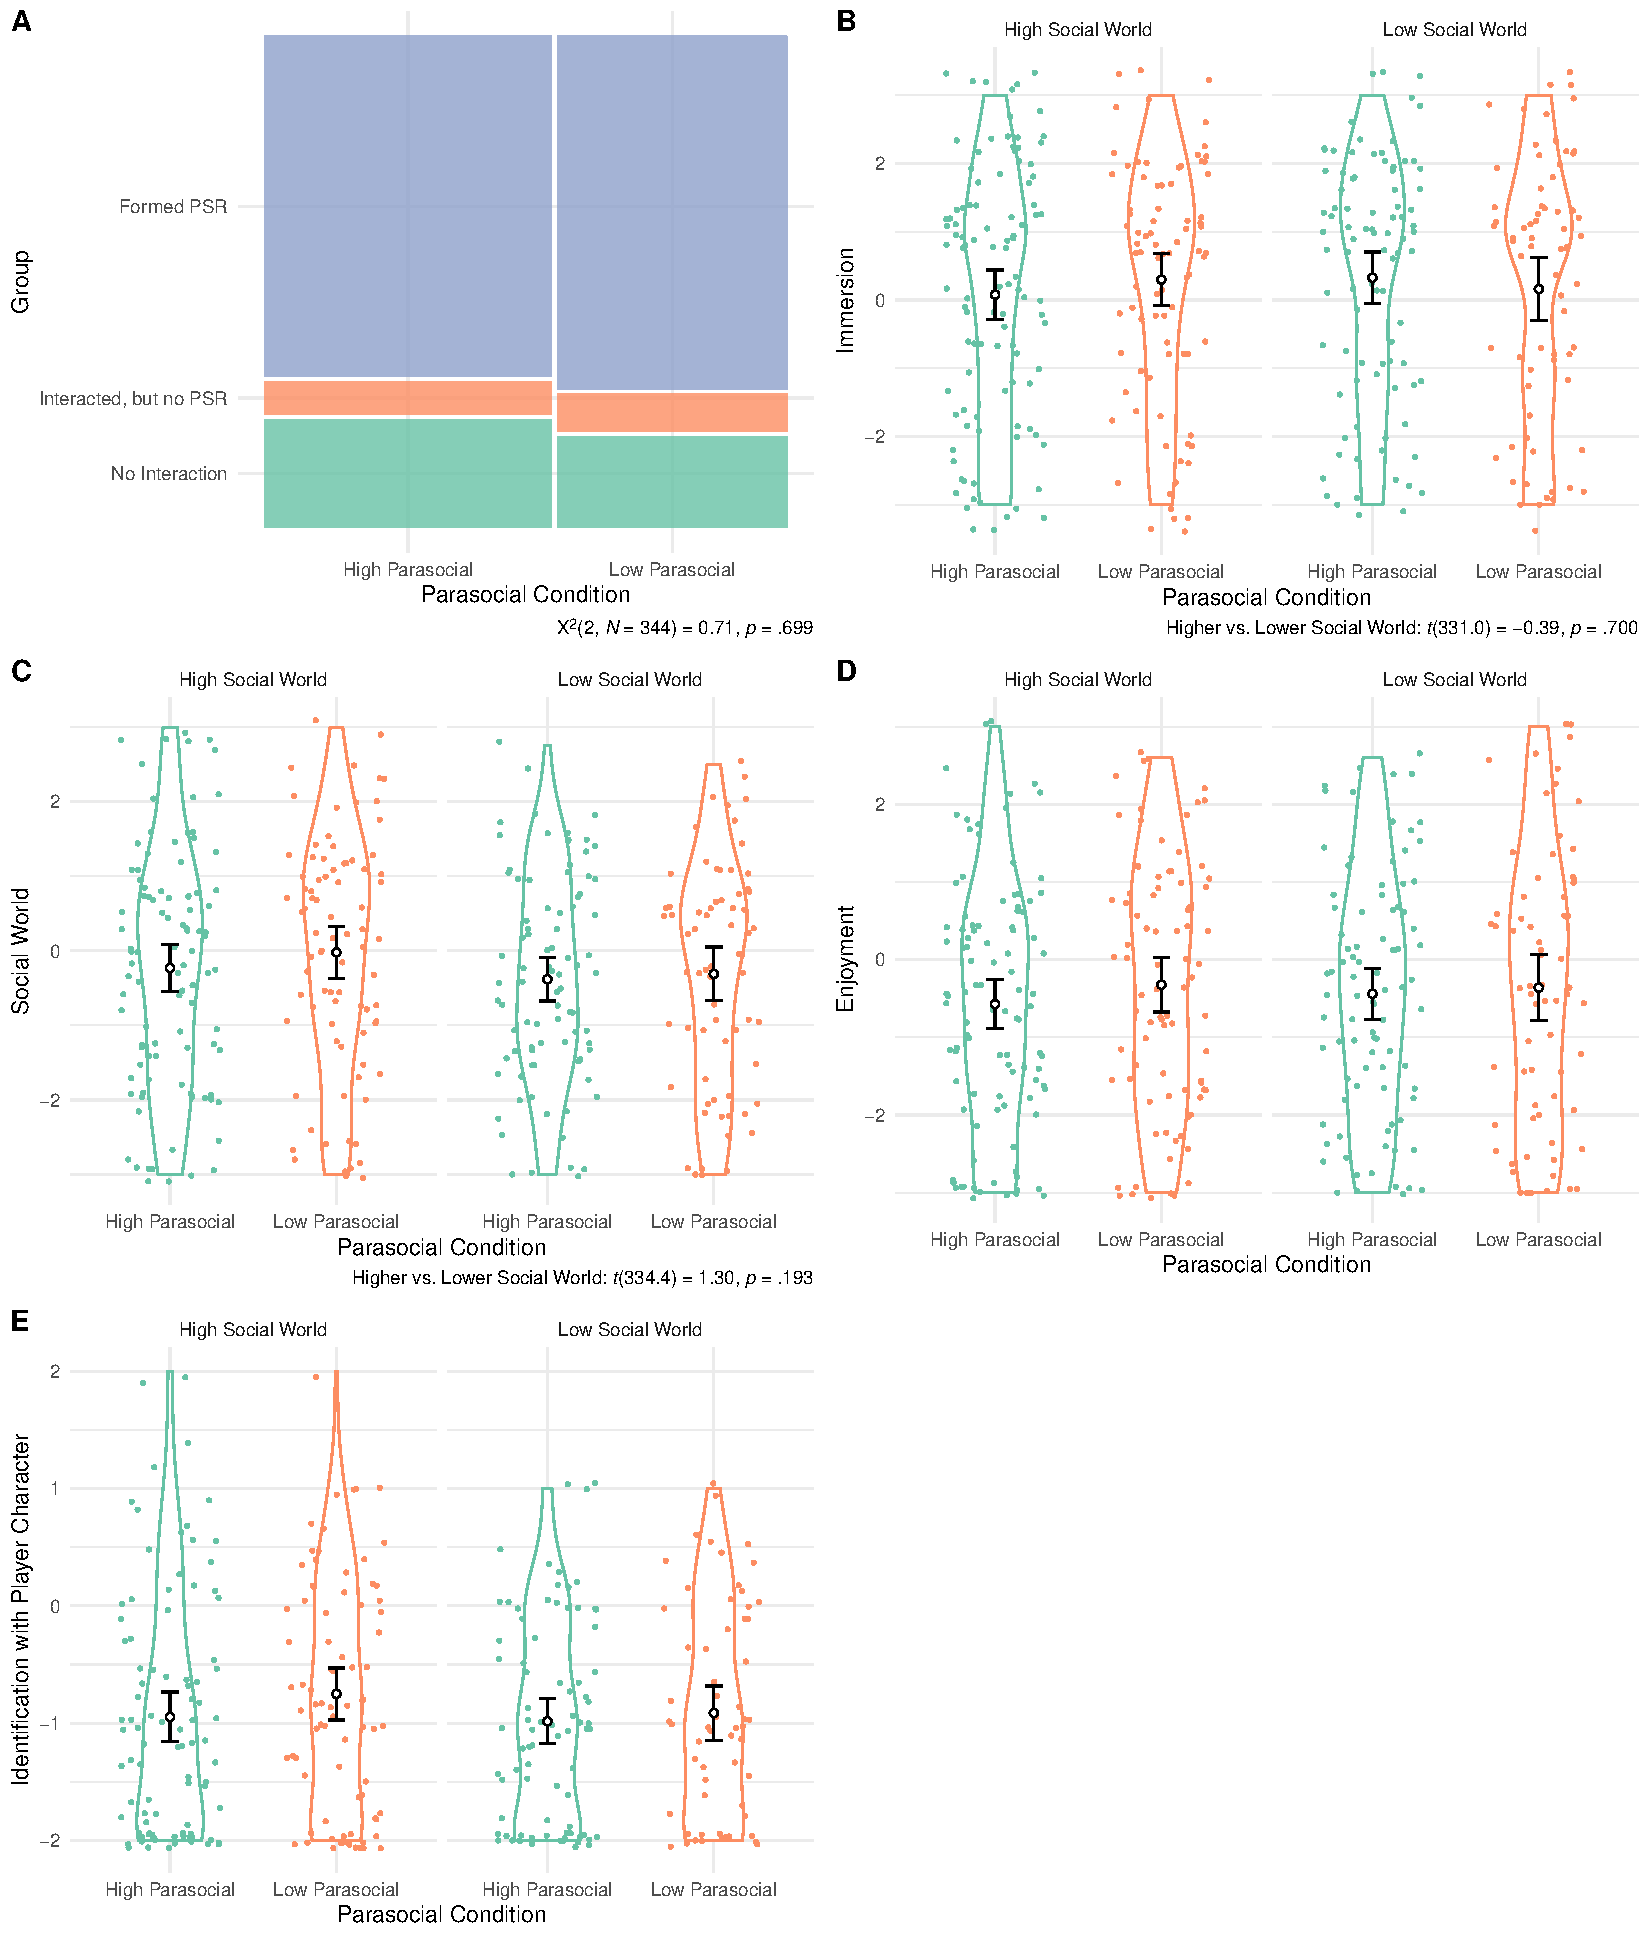
\includegraphics[keepaspectratio]{Sunami-Dissertation_files/figure-latex/s3-exp-manip-check-plot-1.pdf}}
\caption{\label{fig:s3-exp-manip-check-plot}Study 3 - Exploratory Manipulation Check}
\end{figure}

\textbf{Enjoyment Across Conditions.} I explored whether participants
reported different levels of enjoyment after playing the video game
across the condition using a 2 (Parsocial: Higher vs.~Lower) x 2 (Social
World: Higher vs.~Lower) ANOVA on enjoyment scores. Results showed no
main effect of Parasocial Relationships
(\emph{F}(1, 338) = 1.08, \emph{p} = .299), no main effect of Social World
(\emph{F}(1, 338) = 0.32, \emph{p} = .573), and no 2-way interaction bweten
Parasocial Relationships and Social World
(\emph{F}(1, 338) = 0.23, \emph{p} = .633) on enjoyment scores.
Thus, participant's enjoyment did not differ depending on the parasocial
relationships content or the social world content in the video game.

\textbf{Exploratory Moderation Analysis.} I explored whether the gender or
race of participants moderated the effect of the parasocial
relationships and the social worlds on belonging using regression
models. For each demographic characteristic, I constructed a regression
model predicting belonging with the following predictors: Parasocial
Relationships (.5 = high, -.5 = low), Social Worlds (.5 = high, -.5 =
low), Gender (.5 = female, -.5 = male) or Race (four dummy variables
representing: American-Indian, African American/Black, White/Caucasian,
Asian, Pacific Islander, and other), and their fully-crossed interaction
terms. For the moderation anaysis with gender, I did not find the main
effects (Parasocial Relationships:
\emph{B} = -0.14, \emph{SE} = 0.19, \emph{t} = -0.78, \emph{p} = .438, Social World:
\emph{B} = -0.19, \emph{SE} = 0.19, \emph{t} = -1.00, \emph{p} = .317, Gender:
\emph{B} = -0.19, \emph{SE} = 0.19, \emph{t} = -1.00, \emph{p} = .317), the 2-way interactions
(Parasocial Relationships x Gender:
\emph{B} = 0.05, \emph{SE} = 0.37, \emph{t} = 0.13, \emph{p} = .897; Social
World x Gender:
\emph{B} = 0.15, \emph{SE} = 0.37, \emph{t} = 0.39, \emph{p} = .696), or
the 3-way interaction among Parasocial Relationship, Social World, and
Gender
(\emph{B} = -0.53, \emph{SE} = 0.75, \emph{t} = -0.71, \emph{p} = .479).
For the moderation analysis with race, I did not find the main effects,
the 2-way interactions (Parasocial relationships x Social World,
Parasocial Relationships x Race, or Social World x Race), or the 3-way
interaction (Parasocial Relationships x Social World x Race). Note that
only few participants identified as non-White, and thus I was not able
to properly test the moderation by race in this study. Overall, these
results suggest that the effects of the parasocial relationship or
social world were not moderated by gender or racial identities.

\begin{figure}
\centering
\pandocbounded{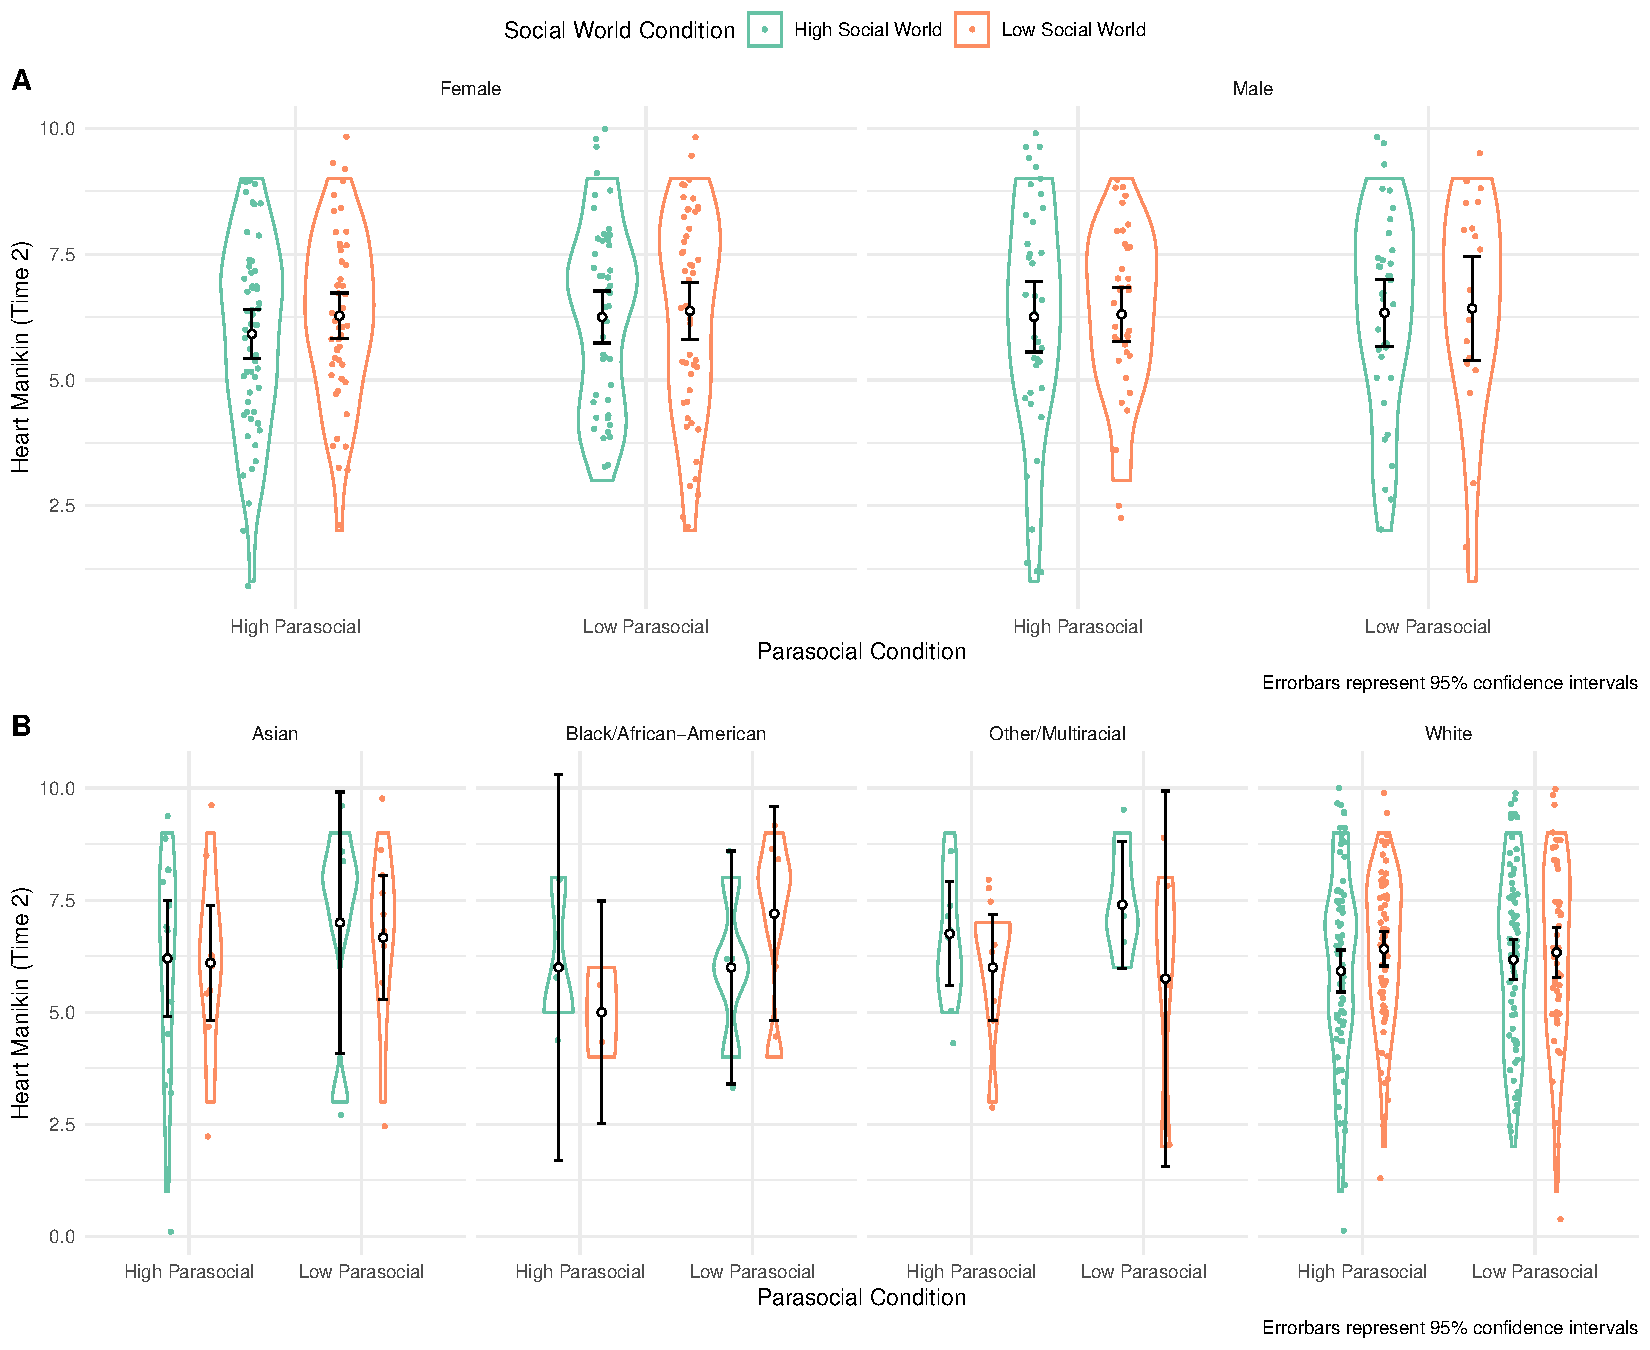
\includegraphics[keepaspectratio]{Sunami-Dissertation_files/figure-latex/s3-moderation-analyses-plots-1.pdf}}
\caption{\label{fig:s3-moderation-analyses-plots}Study 3 - Moderation Analysis. Panel A shows the results for gender. Panel B shows the results for gender. Results showed that gender or racial identities did not moderate the results.}
\end{figure}

\subsection{Unplanned Analyses}\label{unplanned-analyses-1}

\textbf{Exploratory Analyses on Manikin Measures across Time and Condtiions}
Similar to Study 2, I probed whether participants reported different
levels of Heart, Valence, Arousal, and Dominance Manikin scores using a
2 (Parasocial Relationship: Higher vs.~Lower) x 2 (Social World: Higher
vs.~Lower) x 2 (Time: 1 vs 2) mixed-ANOVAs. Across the outcomes, there
were no main effect of parasocial realationship (Heart:
\emph{F}(1, 340) = 0.75, \emph{p} = .386, \(\eta^2_{G}\) = .002; Valence:
\emph{F}(1, 340) = 2.06, \emph{p} = .152, \(\eta^2_{G}\) = .004; Arousal:
\emph{F}(1, 340) = 0.82, \emph{p} = .366, \(\eta^2_{G}\) = .002; Dominance:
\emph{F}(1, 338) = 0.39, \emph{p} = .531, \(\eta^2_{G}\) \textless{} .001) and no main effect of
social world (Heart: \emph{F}(1, 340) = 1.92, \emph{p} = .167, \(\eta^2_{G}\) = .005;
Valence: \emph{F}(1, 340) = 0.47, \emph{p} = .492, \(\eta^2_{G}\) \textless{} .001; Arousal:
\emph{F}(1, 340) = 2.65, \emph{p} = .105, \(\eta^2_{G}\) = .006; Dominance:
\emph{F}(1, 338) = 0.20, \emph{p} = .658, \(\eta^2_{G}\) \textless{} .001). Also, I foud no 2-way
Parasocial Relationship x Social World interaction (Heart:
\emph{F}(1, 340) = 0.10, \emph{p} = .758, \(\eta^2_{G}\) \textless{} .001; Valence:
\emph{F}(1, 340) = 0.01, \emph{p} = .904, \(\eta^2_{G}\) \textless{} .001; Arousal:
\emph{F}(1, 340) = 0.41, \emph{p} = .523, \(\eta^2_{G}\) \textless{} .001; Dominance:
\emph{F}(1, 338) = 1.71, \emph{p} = .192, \(\eta^2_{G}\) = .004), no 2-way
Parasocial Relationship x Time interaction (Heart:
\emph{F}(1, 340) = 0.07, \emph{p} = .786, \(\eta^2_{G}\) \textless{} .001; Valence:
\emph{F}(1, 340) = 0.13, \emph{p} = .719, \(\eta^2_{G}\) \textless{} .001; Arousal:
\emph{F}(1, 340) = 0.87, \emph{p} = .352, \(\eta^2_{G}\) \textless{} .001; Dominance:
\emph{F}(1, 338) = 0.35, \emph{p} = .554, \(\eta^2_{G}\) \textless{} .001), no 2-way Social
World x Time interaction (Heart:
\emph{F}(1, 340) = 0.62, \emph{p} = .433, \(\eta^2_{G}\) \textless{} .001; Valence:
\emph{F}(1, 340) = 0.15, \emph{p} = .701, \(\eta^2_{G}\) \textless{} .001; Arousal:
\emph{F}(1, 340) = 1.39, \emph{p} = .239, \(\eta^2_{G}\) \textless{} .001; Dominance:
\emph{F}(1, 338) = 0.01, \emph{p} = .940, \(\eta^2_{G}\) \textless{} .001), or no 3-way
Parasocial Relationship x Social World x Time interaction (Heart:
\emph{F}(1, 340) = 2.30, \emph{p} = .131, \(\eta^2_{G}\) \textless{} .001; Valence:
\emph{F}(1, 340) = 2.27, \emph{p} = .133, \(\eta^2_{G}\) = .002;
Arousal:
\emph{F}(1, 340) = 0.47, \emph{p} = .495, \(\eta^2_{G}\) \textless{} .001;
Dominance:
\emph{F}(1, 338) = 0.07, \emph{p} = .788, \(\eta^2_{G}\) \textless{} .001).
However, there was a consistent Time effect across the models. At Time
2, Participants reported lower belonging (Time 1:
\emph{M} = 6.45, \emph{SD} = 1.90; Time 2: \emph{M} = 6.24, \emph{SD} = 1.87; \emph{F}(1, 340) = 6.62, \emph{p} = .011, \(\eta^2_{G}\) = .003), lower valence
(Time 1: \emph{M} = 6.00, \emph{SD} = 1.91; Time 2: \emph{M} = 5.64, \emph{SD} = 2.30; \emph{F}(1, 340) = 7.26, \emph{p} = .007, \(\eta^2_{G}\) = .007),
higher arousal (Time 1: \emph{M} = 4.24, \emph{SD} = 1.76; Time 2:
\emph{M} = 5.01, \emph{SD} = 1.97; \emph{F}(1, 340) = 51.70, \emph{p} \textless{} .001, \(\eta^2_{G}\) = .042), and higher dominance (Time 1:
\emph{M} = 6.04, \emph{SD} = 1.63; Time 2: \emph{F}(1, 338) = 4.89, \emph{p} = .028, \(\eta^2_{G}\) = .004)
compared with the baseline (Time 1).

\begin{figure}
\centering
\pandocbounded{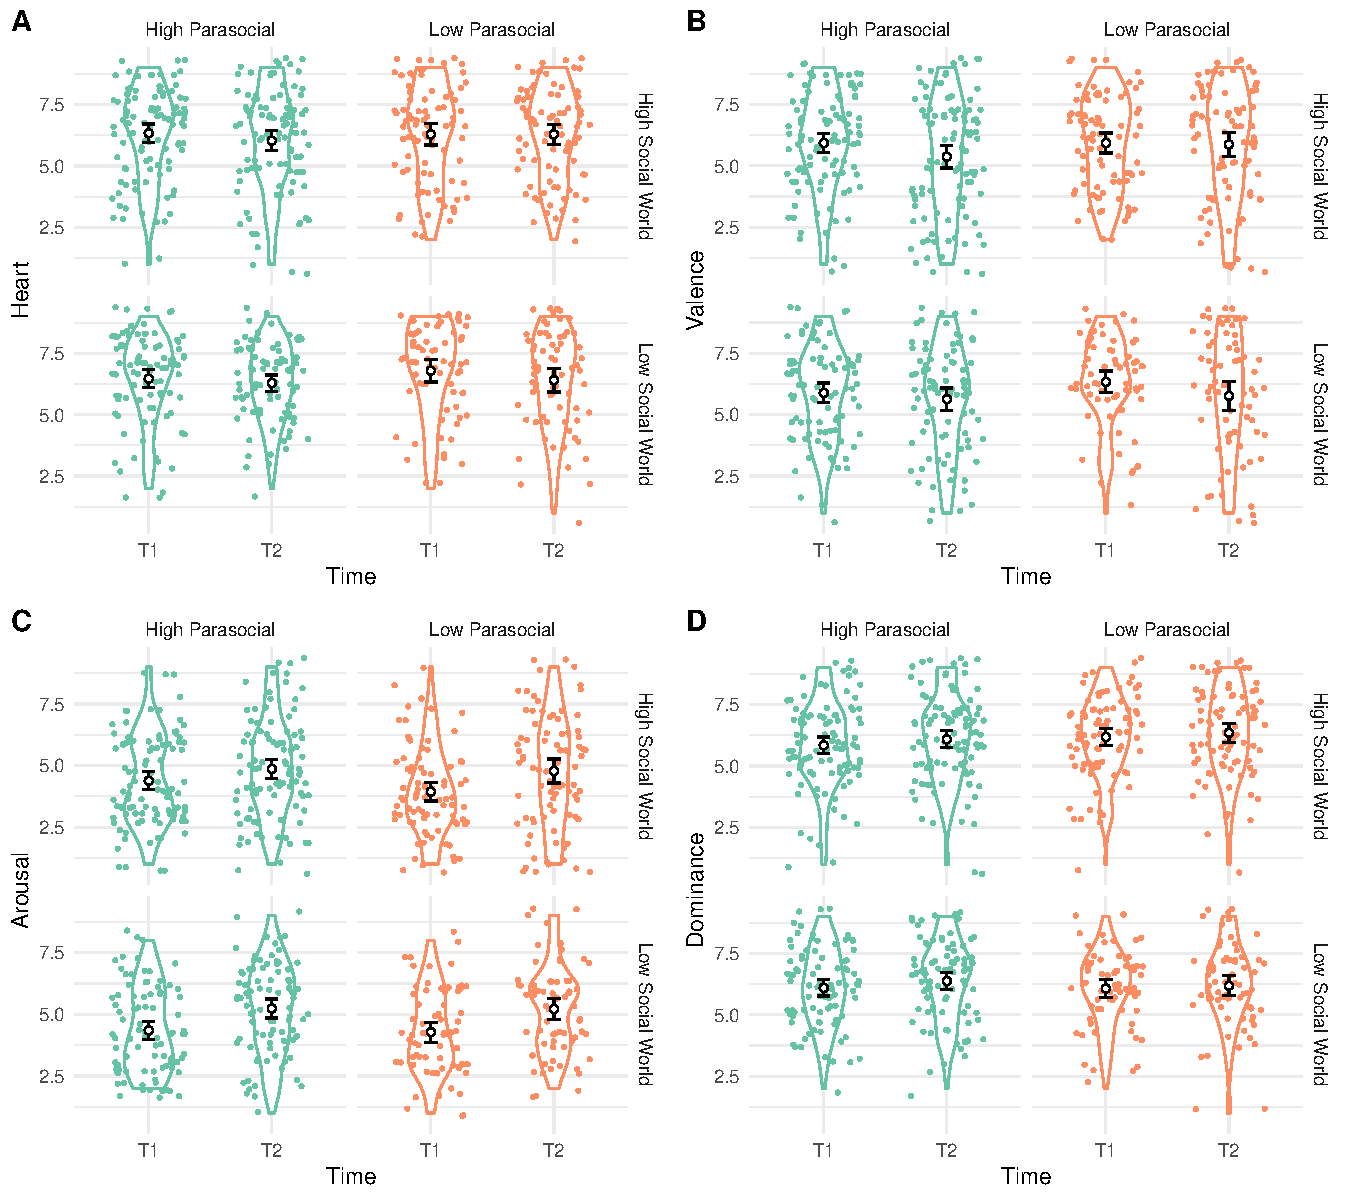
\includegraphics[keepaspectratio]{Sunami-Dissertation_files/figure-latex/s3-manikin-across-time-plot-1.pdf}}
\caption{\label{fig:s3-manikin-across-time-plot}Study 3 - Mankin Scores Across Time By Conditions}
\end{figure}

\textbf{Player Character Identification}. I explored whether participants
reported different levels of identifications with the player characters
across the higher vs.~lower parasocial and social world conditions in a
2 (Parasocial Relationships: Higher vs.~Lower) x 2 (Social World: Higher
vs.~Lower) ANOVA. Results showed that all terms were null (the
parasocial relationships main effect:
\emph{F}(1, 311) = 1.80, \emph{p} = .181, the main effect of social world:
\emph{F}(1, 311) = 0.06, \emph{p} = .803; the interaction between
parasocial relationships and social world:
\emph{F}(1, 311) = 0.34, \emph{p} = .561). These results
suggest that participants reported similar levels of identification with
the player character (Higra) across the conditions.

\textbf{Moderation by Parasocial Relationships, Social World, Enjoyment, and
Player Character Identification}. I explored whether measures of
parasocial relationship, social world, or enjoyment moderated the
effects of the social surrogacy essay manipulation on Heart Manikin a
series of mixed models. I constructed a mixed model for each moderator
variable (the manipulation check groups (Groups 1-3), Inclusion of the
Other in Self Scale, Single-Item Immersion Scale, and the On-The-Fly
Measure of Social World, the Enjoyment Scale, and the Player Character
Identification Scale) Thus, each model contained the following fixed
predictors: the moderator, Parasocial Relationships (higher vs.~lower),
Social World (higher vs.~lower), Time, the 2-way Moderator x Parasocial
Relationships, the 2-way Moderator x Social World interaction, the 2-way
Time x Parasocial Relationships, and the 2-way Time x Social World
interaction, the 3-way Moderator x Parasocial Relationships x Social
World interaction, and the 3-way Parasocial Relatioships x Social World
x Time. (Figure \ref{fig:s3-mod-plots}) Below, I only report positive
results (\emph{p} \textless{} .05) for the heart manikin here for brevity. Note that
these results were not preregistered and thus prone to Type I error.

\begin{figure}
\centering
\pandocbounded{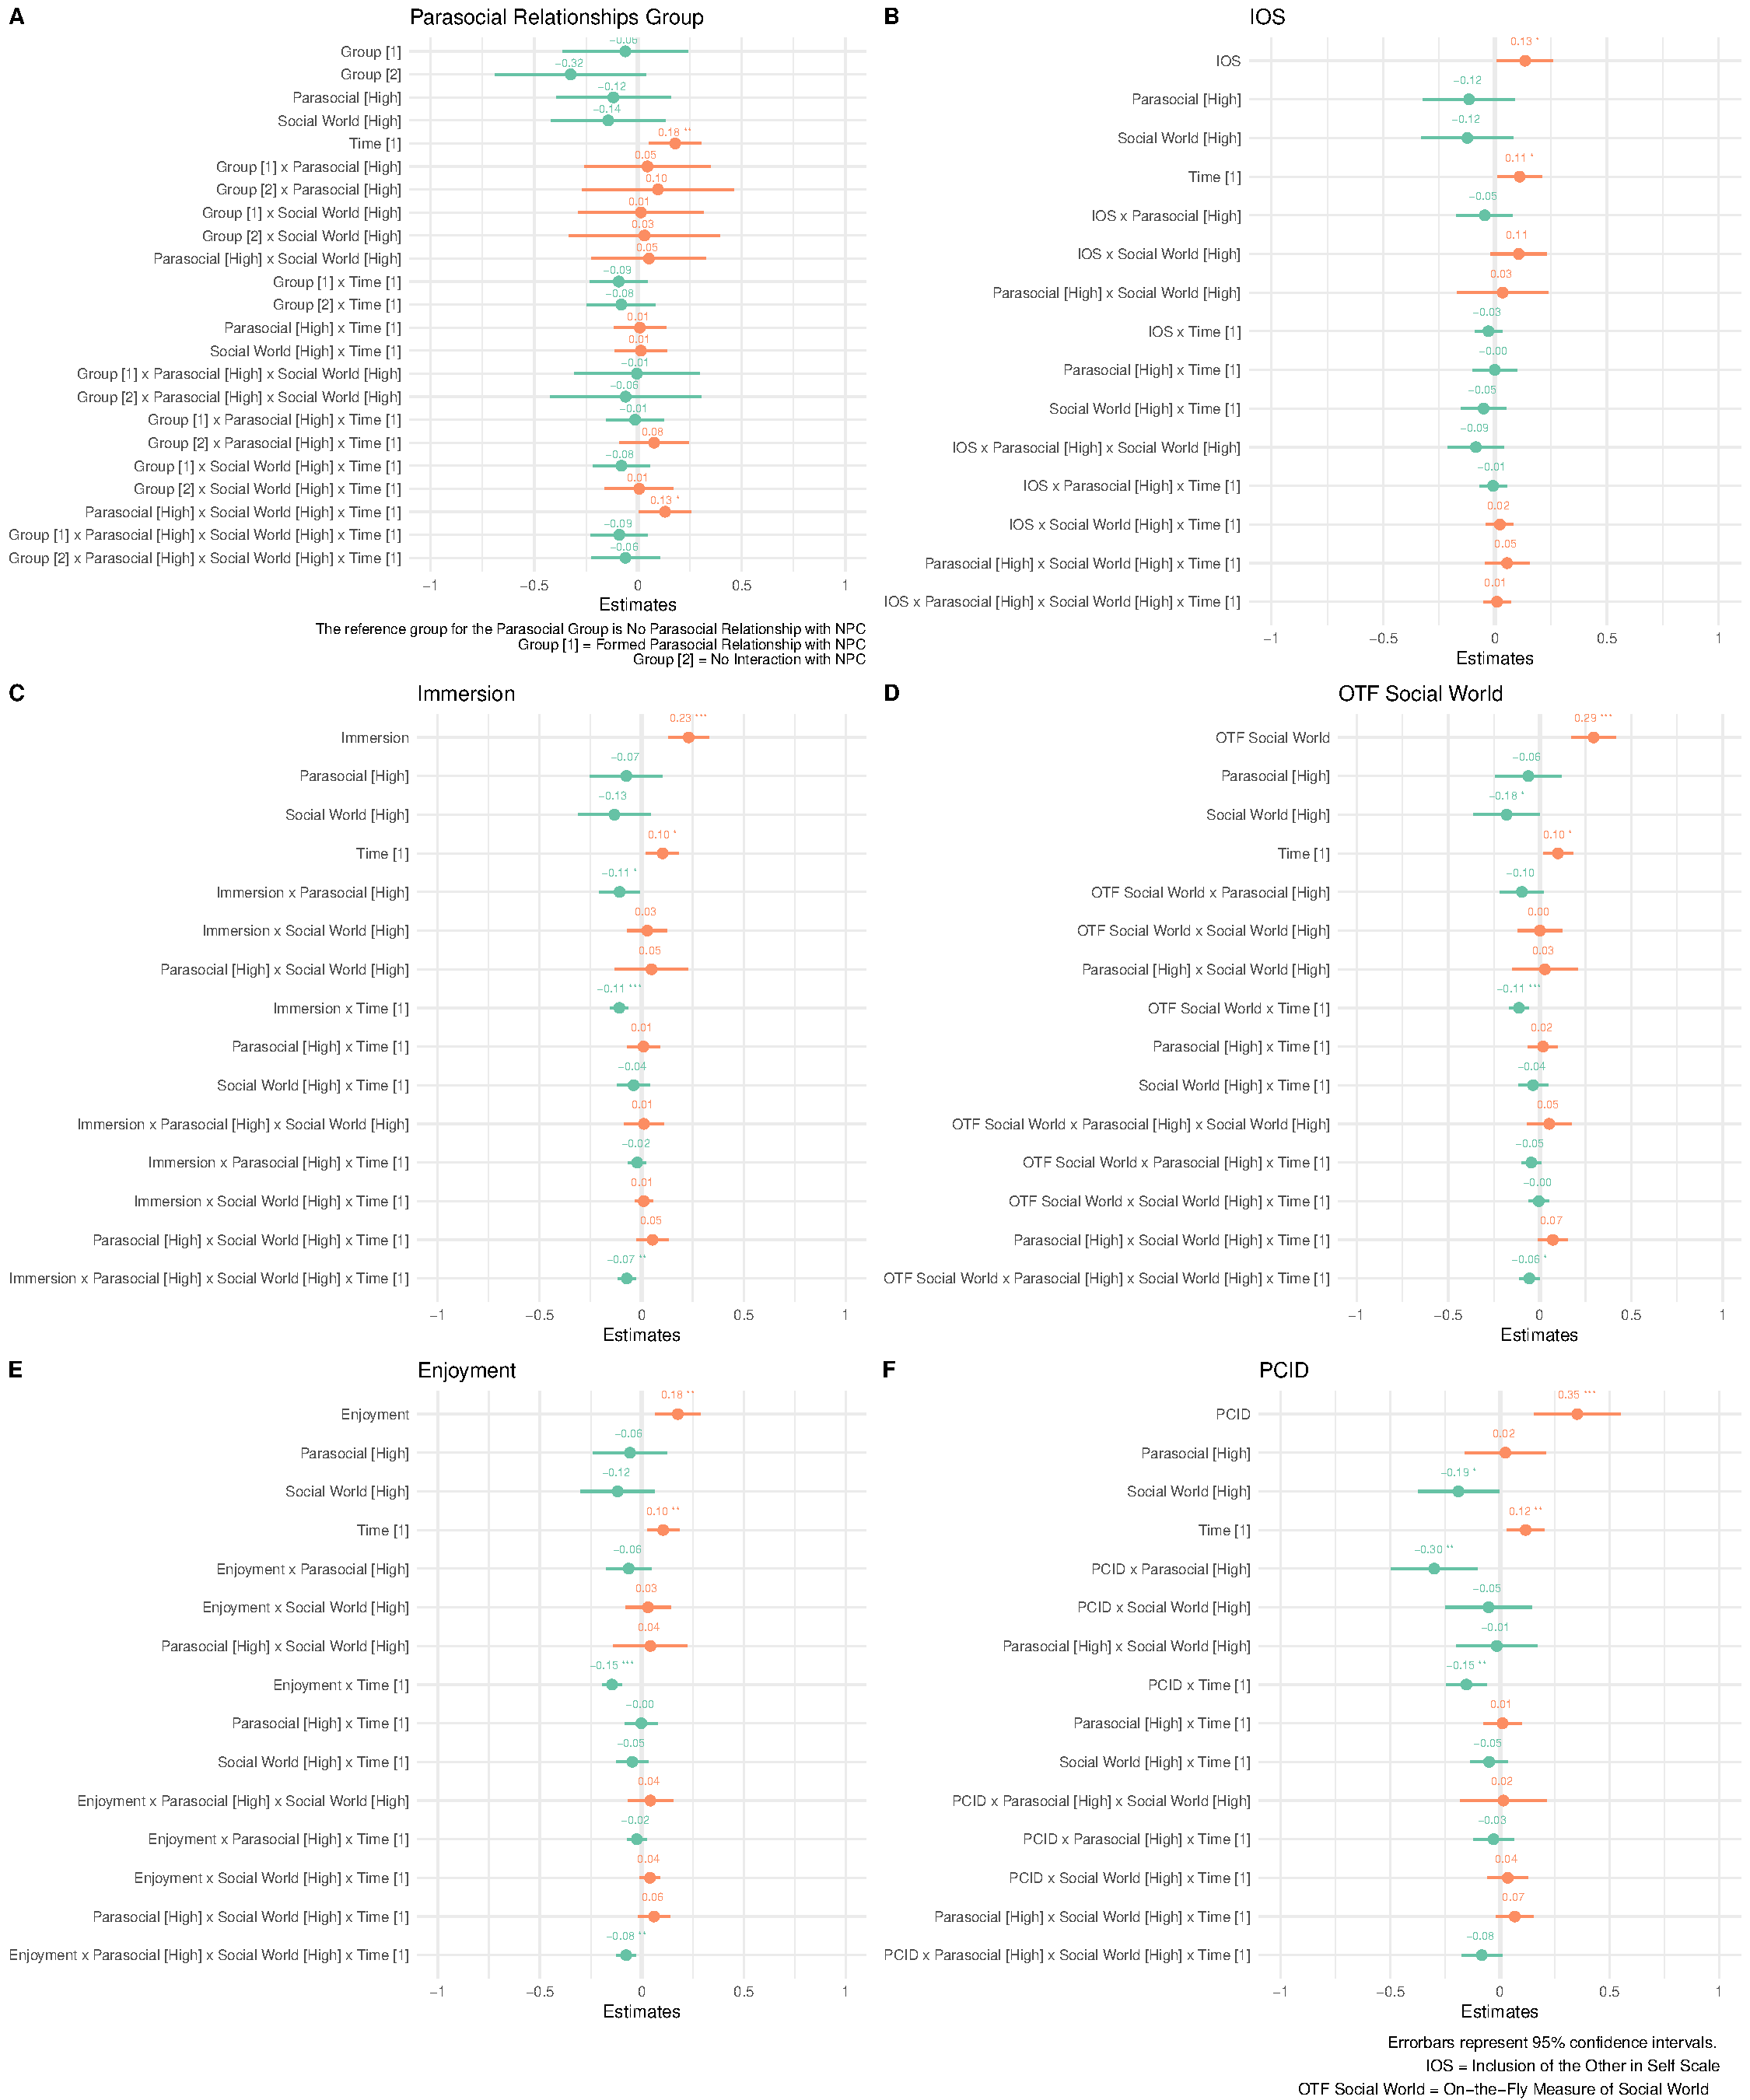
\includegraphics[keepaspectratio]{Sunami-Dissertation_files/figure-latex/s3-mod-plots-1.pdf}}
\caption{\label{fig:s3-mod-plots}Study 3 - Regression Coefficients Across Models Examining Moderation by Parasocial Relationships, Social World, Enjoyment, and Player Character Identification}
\end{figure}

Across all the models, I observed a main effect of time such that
participants reported lower Heart Manikin scores at Time 2 than Time 2,
consistent with the prior analysis.

For the analysis treating parasocial relationship group as a moderator,
I found the three-way interaction among parasocial relationships
condition, social world condition and time
(\emph{B} = 0.13, \emph{SE} = 0.06, \emph{t} = 2.06, \emph{p} = .040;
Figure \ref{fig:s3-mod-plots}, Panel A).
However, follow-up tests showed that the group means were not different
from each other.

For the analysis treating the Inclusion of the Other in Self as a
moderator, I found the main effect of the Inclusion of the Other in Self
scores (\emph{B} = 0.13, \emph{SE} = 0.06, \emph{t} = 2.10, \emph{p} = .037; Figure
\ref{fig:s3-mod-plots}, Panel B). These results suggest that
participants with higher Inclusion of the Other in Self scores reported
higher Heart Manikin sores across conditions and time.

For the analysis treating the Single-Item Immersion scale as a
moderator, I found the main effect of the immersion scores, such that
participants reporting higher immersion also reported higher belonging
(\emph{B} = 0.23, \emph{SE} = 0.05, \emph{t} = 4.61, \emph{p} \textless{} .001; Figure
\ref{fig:s3-mod-plots}, Panel C). I found the two-way Immersion x
Parasocial Relationship Condition effect (
\emph{B} = -0.11, \emph{SE} = 0.05, \emph{t} = -2.16, \emph{p} = .032).
Follow-up tests suggested that the relationship between immersion and belonging was
greater in the low parasocial relationship condition than in the high parasocial relationship condition
(Low Parasocial Relationship Condition: \emph{B} = 0.34, \emph{SE} = 0.07, 95\%CI{[}0.19, 0.48{]}; High Parasocial Relationship Condition: \emph{B} = 0.12, \emph{SE} = 0.07, 95\%CI{[}-0.01, 0.25{]}).
I also found the two-way Immersion x Time
effect
(\emph{B} = -0.11, \emph{SE} = 0.02, \emph{t} = -4.86, \emph{p} \textless{} .001).
Follow-up tests showed that the slope of immersion scores predicting
belonging was greater at Time 2 than Time 1 (Time 1:
\emph{B} = 0.12, \emph{SE} = 0.05, 95\%CI{[}0.01, 0.23{]}; Time 2: \emph{B} = 0.34, \emph{SE} = 0.05, 95\%CI{[}0.23, 0.45{]}). I also found
the four-way Immersion x Parasocial Relationship x Social World x Time
interaction
(\emph{B} = -0.07, \emph{SE} = 0.02, \emph{t} = -3.25, \emph{p} = .001).
Follow-up tests suggested that, among the high parasocial and high
social world condition, the relationship between immersion and belonging
was greater at Time 2 than Time 1 (Time 1:
\emph{B} = -0.03, \emph{SE} = 0.10, 95\%CI{[}-0.23, 0.16{]};
Time 2:
\emph{B} = 0.35, \emph{SE} = 0.10, 95\%CI{[}0.16, 0.55{]}).

For the analysis treating the On-the-Fly Measure of Social World (OTF
Social World) as a moderator, I found the main effect of the On-the-Fly
Measure of Social World, such that participants reporting higher scores
of social world also reported higher belonging
(\emph{B} = 0.29, \emph{SE} = 0.06, \emph{t} = 4.83, \emph{p} \textless{} .001; Figure
\ref{fig:s3-mod-plots}, Panel D). I also
found the main effect of social world, such that participants in the
high social world condition reported lower belonging than those in the
low social world condition
(\emph{B} = -0.18, \emph{SE} = 0.09, \emph{t} = -1.97, \emph{p} = .049). I also
observed the two-way OTF Social World x Time interaction
(\emph{B} = 0.10, \emph{SE} = 0.04, \emph{t} = 2.41, \emph{p} = .016). Follow-up tests
suggested that the relationship between the social world scores and
belonging was greater at Time 2 than at Time 1 (Time 1:
\emph{B} = 0.18, \emph{SE} = 0.07, 95\%CI{[}0.05, 0.31{]}; Time 2: \emph{B} = 0.41, \emph{SE} = 0.07, 95\%CI{[}0.28, 0.54{]}).
Finally, I found the four-way Parasocial Relationships x Social World x
OTF Social World x Time interaction
(\emph{B} = -0.06, \emph{SE} = 0.03, \emph{t} = -2.04, \emph{p} = .042).
Follow-up tests suggested that, in the high parasocial and high social
world condition, the relationship between OTF Social World scores and
belonging was greater at Time 2 than at Time 1 (Time 1:
\emph{B} = 0.03, \emph{SE} = 0.12, 95\%CI{[}-0.20, 0.26{]};
Time 2:
\emph{B} = 0.47, \emph{SE} = 0.12, 95\%CI{[}0.24, 0.70{]}).

For the analysis treating the enjoyment as a moderator, I found the main
effect of enjoyment, such that participants with higher scores of
enjoyment reported higher belonging
(\emph{B} = 0.18, \emph{SE} = 0.06, \emph{t} = 3.11, \emph{p} = .002; Figure
\ref{fig:s3-mod-plots}, Panel E). I also found the
2-way Enjoyment x Time interaction
(\emph{B} = -0.15, \emph{SE} = 0.02, \emph{t} = -5.92, \emph{p} \textless{} .001). Follow-up
tests suggested that the relationship between enjoyment and belonging
was greater at Time 2 than at Time 1 (Time 1:
\emph{B} = 0.03, \emph{SE} = 0.06, 95\%CI{[}-0.09, 0.15{]}; Time 2:
\emph{B} = 0.32, \emph{SE} = 0.06, 95\%CI{[}0.20, 0.44{]}). I also observed the four-way
Enjoyment x Parasocial Relationships x Socail World x Time interaction
(\emph{B} = -0.08, \emph{SE} = 0.02, \emph{t} = -3.09, \emph{p} = .002).
Follow-up tests showed that, in the low parasocial and low social world
condition, the relationship between enjoyment and belonging was greater
at Time 2 than at Time 1 (Time 1:
\emph{B} = -0.02, \emph{SE} = 0.12, 95\%CI{[}-0.25, 0.21{]};
Time 2:
\emph{B} = 0.39, \emph{SE} = 0.12, 95\%CI{[}0.16, 0.62{]}).
The relationship between enjoyment and belonging in the low parasocial
and low social world at Time 2 was also greater than the relationship
between enjoyment and belonging in the high parasocial and low social
world condition at Time 1
(\emph{B} = 0.39, \emph{SE} = 0.12, 95\%CI{[}0.16, 0.62{]}
vs.
\emph{B} = -0.10, \emph{SE} = 0.13, 95\%CI{[}-0.34, 0.15{]}).

Lastly, for the analysis treating the identification with the player
character as a moderator, I found the main effect of the player character
identification, such that participants who identified more with the
player character reported higher belonging across conditions and time
(\emph{B} = 0.35, \emph{SE} = 0.10, \emph{t} = 3.51, \emph{p} \textless{} .001; Figure
\ref{fig:s3-mod-plots}, Panel F). I
also found the main effect of Social World, such that participants in the
High Social World condition reported lower belonging
(\emph{B} = -0.19, \emph{SE} = 0.09, \emph{t} = -2.02, \emph{p} = .045). The two-way
player character identification x Parasocial Relationships was greater
than zero
(\emph{B} = -0.30, \emph{SE} = 0.10, \emph{t} = -2.99, \emph{p} = .003).
Follow-up tests suggested that the relationship between player character
identification and belonging was greater in the low parasocial condition
than in the high parasocial condition (low parasocial condition:
\emph{B} = 0.65, \emph{SE} = 0.15, 95\%CI{[}0.36, 0.95{]}; high parasocial
condition: \emph{B} = 0.05, \emph{SE} = 0.13, 95\%CI{[}-0.21, 0.32{]}). I also
found the two-way Player Character Identification x Time interaction
(\emph{B} = -0.15, \emph{SE} = 0.05, \emph{t} = -3.27, \emph{p} = .001).
Follow-up tests suggested that the relationship between player character
identification and belonging was stronger at Time 2 than at Time 1 (Time
1: \emph{B} = 0.20, \emph{SE} = 0.11, 95\%CI{[}-0.02, 0.42{]}; Time 2:
\emph{B} = 0.51, \emph{SE} = 0.11, 95\%CI{[}0.29, 0.72{]}).

\textbf{Bivariate Correltion Analysis}. I explored associations among the
measured variables via bivariate correlations. I only report select
positive associations here. For the full correlation matrix, see Table
\ref{tab:appendix-s3-correlations-table} in {[}Appendix{]}. Note that these
analyses were not planned a priori, and prone to Type I error. At Time
2, participants with higher Heart Manikin scores reported higher
parasocial relatioships, immersion, social world, player character
identification, and enjoyment, compared with those with lower Heart
Manikin scores. Measures of parasocial relationships, immersion, social
world, player character identification, and enjoyment were positively
correlated with each other.

\section{Discussion}\label{discussion-2}

In Study 3, I tested whether playing a video game with higher parasocial
relationships and higher social worlds could increase belonging
following social rejection (Hypotheses 2, 3, and 4). Results did not
support these hypothesis. Rejected participants reported similar levels
of belonging regardless of the levels of exposure to the parasocial
relationships content and the social world content in the video game.
The current null results imply many possibilities: (a) failure of
manipulating parasocial relationships and social worlds, (b) failure of
inducing social rejection, (c) time passed from social rejection simply
recovering belonging, and (d) stressors and distractions during the
COVID-19 pandemic reducing the effectiveness of the rejection induction
and the social surrogacy manipulations.

\textbf{Failure of Manipulating Parasocial Relationships and Social Worlds}
We can possibly attribute the current results to ineffective
manipulations for the parasocial relationships and social worlds.
Results of the exploratory manipulation check supports this notion.
Regardless of their parasocial condition, participants reported similar
levels of experiencing parasocial relationships. Similarly, participants
reported similar levels of social world regardless of the social world
conditions (higher vs lower). As planned, I refrain from making a
conclusion about the effectiveness of the manipulations since the
manipulation check measures were not validated to measure parasocial
relationships and social worlds, as mentioned previously. Still, these
null results highlight the possibility of the failure of the
manipulations.

In retrospect, a better approach would have been to validate the
effectiveness of the video game manipulation with the social world. That
said, these measures have never been used to validate the effectiveness
of a manipulation for parasocial relationships and social world, and
thus the true effectiveness of the current manipulation remains
ambiguous. Future studies should develop effective measures of prosocial
relationships and social world, and then use them to validate
manipulations.

\textbf{Failure of Inducing Social Rejection.} Consistent with the
possibility discussed in Study 2, the rejection manipulation could have
been ineffective to begin with, and thus the current study failed to
capture any effects of recovering belonging. Again, I suggest that this
possibility is unlikely since the rejection manipulation was shown to be
effective, as discussed in Study 2.

\textbf{Time from Rejection Induction} Participants played the video game on
the average of 30.48 minutes
(\emph{M} = 30.48, \emph{SD} = 63.69). One possibility is that all participants
replenished their belonging while playing the video game, regardless of
their parasocial relationships and social world content. If this is the
case, participants would report similar levels of belonging before
writing the rejection essay and after playing the video game. However,
the results do not support this notion. Instead, participants felt less
belonging after playing a game (Time 2) than their baseline (Time 1). I
cannot conclude whether passage of time replenished everyone's belonging
based on the current results.

\textbf{Negative Effect of Video Game on Belonging}. One possibility remains
that the video game had a negative, not a positive, effect on belonging.
Again, participants reported lower belonging after playing the video
game (Time 2) than baseline. I speculate two possibilities for the
lowered belonging: (a) frustrations in playing a new game, and (b)
fighting with enemies.

I speculate that some participants may have experienced frustrations in
completing the game (e.g., difficulty in controls) since everyone played
the game for the first time. As a result, participants may have
experienced lowered sense of control. Since people with lowered sense of
control can experience lowered belonging, participants who experienced
difficulty playing the game could have experienced lowered sense of
belonging (\citeproc{ref-williamsOstracismTemporalNeedthreat2009}{Williams, 2009}).

I also speculate that the battles in the game may have had an adverse
influence to a sense of belonging. The role-playing games on the market
usually contain contents of fighting against enemies. Thus, I included
battles in the game to make the current video game representative of
other games on the market. However, battles involve defeating monsters
and key enemy figures, akin to aggressive, antisocial behaviors that
usually reduce belonging. Some participants may have found it aversive
to defeat enemies in the game, especially if they liked the enemy
characters, eventually lowering their sense of belonging.

\textbf{Participants Meta-Experience of the Study due to Pandemic}.
Participants in the current study participated in the study online
during the COVID-19 pandemic (participation date ranging from
March, 2021 to
April, 2021). One possibility of
the null result can be that the basal stresses and social isolation
during the pandemic is so prominent that the social surrogacy
manipulation deemed ineffective, resulting in everyone feeling rejected
regardless of the exposure to social surrogacy. Another possibility is
that these pandemic-related stresses distracted participants from paying
attention in the game, resulting in ineffective manipulations of
parasocial relationships and social worlds. Although I excluded any
participants who failed attention check, these pandemic-related stresses
and distractions might have made participants less affected by the
social surrogacy presented in the manipulations. Overall, I suggest that
we interpret the current results with a caveat that the data collection
happened during a global pandemic.

Overall, results of Study 3 suggested that rejected participants did not
replenish belonging after playing a video game, regardless of their
content of parasocial relationships or social world. These results are
inconsistent with the social surrogacy hypothesis suggesting that
parasocial relationships and social world can replenish belonging. I
speculate that the inconsistencies might stem from the failure of
manipulation social surrogacy (parasocial relationships and social
world), the failure of social rejection, time from rejection experience,
the video game's negative effect on belonging, and the participants'
experience of the study due to the COVID-19 pandemic.

\chapter{General Discussion}\label{general-discussion}

In my dissertation studies (total N = 1970), I examined whether playing a single-player
video game alone replenishes belonging after social rejection, a
potential disengaged--prosocial response to social rejection in the
bi-dimensional rejection taxonomy (\citeproc{ref-sunamiBIDimensionalRejectionTaxonomy2020}{Sunami et al., 2020}). In Study 1, I
validated a single-item measure of belonging, the Heart Manikin, used as
the primary outcome for the subsequent studies. In Study 2, I examined
whether recalling one's time playing a social surrogate video game vs.~a
non-social surrogate video game can replenish belonging after social
rejection. Lastly in Study 3, I examined whether rejected people who
play a video game with varying degrees of parasocial relationship and
social world contents can replenish their belonging. The results of the
studies did not support the social surrogacy hypothesis. I discuss the
implications of the current nulls results below.

\section{Impact on the Social Rejection and Video Games Literature}\label{impact-on-the-social-rejection-and-video-games-literature}

\subsection{Heart Manikin as a Quick Measure of Belonging}\label{heart-manikin-as-a-quick-measure-of-belonging}

In Study 1, I attempted to validate the Heart Manikin. Results indicated
a strong evidence for the convergent validity of the heart manikin with
belonging-related measures, including a sense of belonging, self-esteem,
control, and meaningful existence. The Heart Manikin scores also
converged consistently with measures of positive affect. On the other
hand, I found moderate evidence for the discriminant validity of the
Heart Manikin. The Heart Manikin scores did not correlate with unrelated
constructs, such as interpersonal reactivity, paradoxical mindset, sleep
quality, abuse perpetration, food craving, body image, and subjective
socioeconomic status. However, the measure did not show discriminant
validity against measures of arousal and dominance. Overall, I suggest
that the Heart Manikin has a strong convergent validity with measures of
belonging and positive valence. Future studies in social rejection
research could use this measure to efficiently measure state belonging.
Given the moderate discriminant validity of this measure, I recommend
researchers to use other concurrent measure if they wish to measure
belonging that is independent from arousal, dominance, and possibly
subjective socioeconomic status.

I also tested whether the Heart Manikin scores were sensitive to the
laboratory manipulation of social rejection. Across Studies 1c, 1d, and
1e, I observed that participants in the rejected condition reported
lower Heart Manikin scores than those in the non-rejected condition,
supporting the sensitivity of this measure. I suggest that the Heart
Manikin can be a useful, quick tool to check an effectiveness of a
social rejection manipulation.

\subsection{Possible Explanations for the Null Results and Implications to Social Surrogacy Hypothesis}\label{possible-explanations-for-the-null-results-and-implications-to-social-surrogacy-hypothesis}

The current results are not consistent with the social surrogacy
hypothesis on surface (\citeproc{ref-gabrielSocialSurrogatesRejection2017}{Gabriel \& Valenti, 2017}). In two studies, I observed that
rejected participants did not replenish their belonging after writing
about a video game with social surrogates (compared with writing about a
video game without them), and after playing a novel video game with
higher parasocial relationships and social world content (vs.~low
parasocial relationships and social world content). Below I speculate
why I observed null results.

\textbf{Ineffective Manipulations on Social Surrogacy.} The manipulations for
the social surrogates used in Studies 2 and 3 were new, and thus they
have never been validated to manipulate social surrogacy. That being
said, I expected that these manipulations were reasonable to induce
social surrogacy for the following reasons.

In Study 2, I used a role-playing game for social surrogacy essay since
role-playing games often present strong relatable characters and
immersive stories and social world. I contrasted these games with non
role-playing games that usually do not have these components. In Study
3, I developed a novel role-playing game to independently manipulate
parasocial relationships and social worlds, Since the game was new, I
was able to avoid any influence from participants' previous exposure to
the game's characters or stories.

Yet, I did not observe results consistent with the social surrogacy
hypothesis. To explore the effectiveness of the manipulations, I used
exploratory manipulation checks. Results for the manipulation checks
were inconsistent across Studies 2 and 3. In Study 2, participants
reported higher parasocial relationships and social worlds in the social
surrogacy condition, compared with the non-social surrogacy condition.
In Study 3, participants reported similar levels of parasocial
interactions and social worlds, regardless of the type of the video game
they played. Overall, I do not conclude about the effectiveness of the
manipulations given that the manipulation check items were never used to
validate manipulations. Future studies should investigate how we
effectively induce social surrogacy (parasocial relationships and social
worlds) and how we can measure these constructs in a validated manner.

\textbf{Type II Error.} An absence of an effect does not mean that the true
effect is absent---it can mean Type II error, missing a true effect.
But, I suggest that Type II error is unlikely since (a) I ensured that
all studies were powered to detect an effect of (\emph{d} =
0.35), and (b) the null findings are consistent across
studies. That said, the current studies could only capture an effect
size that is larger than (\emph{d} = 0.35). If the true effect
of social surrogacy on belonging was smaller than this hypothesized
effect size, the current studies could not detect the effect.

\textbf{Towards Refining the Theory.} Another possibility is that the social
surrogacy hypothesis may not be robust in its current form, and the
theory needs to identify boundary conditions and expected effect sizes
of social surrogates on belonging. Empirical evidence supporting the
social surrogacy hypothesis has mainly come from studies on books and TV
programs, but not video games. One possibility is that the social
surrgacy hypothesis operates better in reading books and watching TV
programs, but apply less to playing video games. Future studies should
examine these possibilities.

\subsection{Implications to Video Game Studies}\label{implications-to-video-game-studies}

In the video games literature, accumulating theoretical work and
qualitative evidence suggest that video game players can feel being
connected with characters in the game, and thus satisfying relatedness
needs (\citeproc{ref-bopp2019}{Bopp et al., 2019}; \citeproc{ref-burgess2020a}{Burgess \& Jones, 2020}; \citeproc{ref-poretski2019}{Poretski et al., 2019}; \citeproc{ref-tyack2017}{Tyack \& Wyeth, 2017}). However, no
experimental studies have tested this possibility, and the current
studies offered initial experimental tests of this possibility.

The current null results did not find that participants satisfied
belonging (relatedness needs) by writing about video games (Study 2) or
by playing one (Study 3). However, I did find that participants reported
forming more parasocial relationships with non-player characters, more
immersion, more engagement with the narrative, more social world, and
more enjoyment for a social surrogacy game (e.g., a role-playing game),
compared with a non-social surrogacy game in Study 2. Moreover, people
who enjoyed their video game more reported feeling more belonged and
happier, forming more parasocial relationships with characters, engaged
more with the narrative, and immersed more into the story (see the
bivariate correlation analysis in Study 3). These results at minimum
suggest that belonging, paraoscial relationships, social worlds, and
enjoyment are interrelated in video games.

\section{Possible Impact on Society}\label{possible-impact-on-society}

All humans have a fundamental need to belong, and when this need is
threatened, people experience adverse mental and physical health
outcomes (\citeproc{ref-cacioppoLonelinessSpecificRisk2006}{Cacioppo et al., 2006}; \citeproc{ref-hawkleyLonelinessPredictsIncreased2010}{Hawkley et al., 2010}; \citeproc{ref-jaremkaLonelinessPromotesInflammation2013}{Jaremka, Fagundes, Peng, et al., 2013}). People experience
threats to belonging in everyday life (\citeproc{ref-nezlekOstracismEverydayLife2012}{Nezlek et al., 2012}). Identifying an
effective strategy to replenish belonging after social rejection will
help efforts to develop interventions to protect belonging, and
ultimately improve mental and physical well-being. One step for
identifying such intervention is to measure belonging in a quick and
effective way. The Heart Manikin validated in my dissertation can be an
ideal tool for a large-scale research that requires less cost per
participant.

The current null results for the social surrogacy hypothesis do not
offer clear strategies to reduce threats to belonging. However, I did
find that participants who enjoyed a video game reported higher
belonging compared with those who did not enjoy across studies. Future
studies could explore whether playing an enjoyable video game has a
positive impact on belonging vs playing an unenjoyable video game. Such
evidence could add to the broader conversation about the benefits of
playing a video game (\citeproc{ref-granicBenefitsPlayingVideo2014}{Granic et al., 2014}).

\section{Constraints on Generality and Future Directions}\label{constraints-on-generality-and-future-directions}

I discuss the constraints on generality of the present findings
(\citeproc{ref-simons2017}{Simons et al., 2017}) to highlight any design or sample characteristics that can
impose constraints on interpretation of the results and future
directions in this section.

\subsection{Social Surrogates in Non-Rejected People}\label{social-surrogates-in-non-rejected-people}

Across the current studies (Studies 2 and 3), all participants
experienced acute social rejection before seeing social surrogates.
Thus, the current studies did not test whether non-rejected people can
increase belonging, or whether people with chronic feelings of social
rejection (e.g., loneliness) could replenish belonging via social
surrogacy in video games, both important directions for future
investigations.

\subsection{Negative Parasocial Relationships and Social Worlds}\label{negative-parasocial-relationships-and-social-worlds}

The current studies only examined positive parasocial relationships and
social worlds. In Study 2, participants recalled their parasocial
relationships and social worlds in their favorite game. In Study 3,
participants experienced a friendly parasocial target and a positive
social world. The results of the current study may not generalize to
other video games where people have a negative parasocial relationship
with characters, or negative experience being immersed in a social
world. People can hate characters in TV programs (\citeproc{ref-chory2013}{Chory, 2013}; \citeproc{ref-jennings2016}{Jennings \& Alper, 2016})---likewise, people can hate non-player characters and
form a negative parasocial relationship. People can also immerse
themselves in negative social worlds---social worlds that are immoral or
ethically unjust, such as ones described in many horror films (e.g., the
Saw Franchise, the Texas Chain Saw Massacre, etc.). Future research
should carefully consider the nature of the parasocial relationships and
the social worlds in video games, and whether they can replenish or even
hurt belonging.

\subsection{Another Type of Social Surrogacy: Reminders of Others}\label{another-type-of-social-surrogacy-reminders-of-others}

The social surrogacy hypothesis identifies three types of social
surrogates: parasocial relationships, social worlds, and reminders of
others (\citeproc{ref-gabrielSocialSurrogatesRejection2017}{Gabriel \& Valenti, 2017}). In my dissertation, I focused on parasocial
relationships and social worlds but not reminders of others---remnants
of real social relationships, such as photographs of close others,
comfort foods prepared by loved ones. I did not focus on the remainder
of others because the current definition of reminders of others requires
a real preexisting social relationship that is absent in single-player
video games.

A new avenue for research may be to examine if the definition of
reminders of others includes the parasocial relationship and social
worlds. People can play video games to remind themselves of past
parasocial relationships and social worlds experienced previously in
video games---especially those multiple releases over time. For example,
long-time players of the Animal Crossing series can play a newly
released Animal Crossing: New Horizons in 2020 (\citeproc{ref-nintendo2020a}{E. P. D. Nintendo, 2020}), and
remember about the parasocial relationships they formed with the older
game such as Animal Crossing: New Leaf in 2012 (\citeproc{ref-nintendo2012a}{E. A. D. Nintendo, 2012}).
Similarly, playing Witcher 3 in 2015 (\citeproc{ref-cdprojektred2015}{CD Projekt Red, 2015}) can remind the
player of their time immersed in the social world in the first Witcher
in 2007 (\citeproc{ref-cdprojektred2007}{CD Projekt Red, 2007}). Future studies can examine whether people
can replenish belonging via remainders of the parasocial relationships
or social worlds.

As mentioned in Study 2, I speculate that people may have replenished
belonging by remembering their memories of playing a single-player video
game in the presence of a close other. For example, people can feel
loved by simply remembering their time playing Tetris in front of their
friends. This way, people replenish belonging, not because of the
content of the game, but because of the time shared with their friends.
Future studies that focus on single-player video game can ask
participants to report how much they spend playing a video game in front
of others (e.g., passing controllers to each other, or simply letting
someone watch the game). A novel hypothesis is that participants can
replenish their belonging by remembering a video game that they shared
playing with close others, similar to replenishing belonging via comfort
food (\citeproc{ref-troisiThreatenedBelongingPreference2015}{Troisi et al., 2015}; \citeproc{ref-jordand.troisiChickenSoupReally2011}{Troisi \& Gabriel, 2011}).

\subsection{Character Identification}\label{character-identification}

In the present dissertation, I focused on parasocial relationships with
the non-player characters in video games. However, existing studies
suggest that players can be emotionally attached to the player
characters they control---such as Commander Sheperd in Mass Effect and
Geralt of Rivia in Witcher (\citeproc{ref-bopp2019}{Bopp et al., 2019}). According to the current
definition of a parasocial relationship, the relationship between the
player and the player character may not be considered as parasocial
since the relationship can be two-sided: the player can control and
influence the player character's behavior, which in turn influences the
player's behavior (\citeproc{ref-banks2015}{Banks, 2015}; \citeproc{ref-banks2016}{Banks \& Bowman, 2016}; \citeproc{ref-cohen2014}{J. Cohen, 2014}). Thus, the
relationship players form with the player character may not fall under
the concept of social surrogates. However, players can be emotionally
attached to the player character and thus may replenish their sense of
belonging. Indeed, theoretical discussions suggest that players can form
parasocial relationships with player characters with established
backgrounds (e.g., Lara Croft from the Tomb Raider series), but not with
the avatars that they create themselves {[}e.g., the player character in
Skyrim; Kavli (\citeproc{ref-kavli2012}{2012}); Lewis et al. (\citeproc{ref-lewis2008}{2008}){]}.

I explored the role of player character identification in Study 3. In
general, identification with the player character was unrelated to
belonging. However, among participants who played a game without a
parasocial relationship target, those identifying more with the player
character reported higher belonging than those identifying less with the
player character. This association was absent among participants who
played a game with a parasocial relationship target. One possible
explanation for these results is that participants identifying with the
player character (Higra) were more likely to experience higher belonging
in an absence of the parasocial target (Sashu) since the player can
focus more on the player character. On the other hand, in the higher
parasocial relationship condition, players' attention was divided
between the player character and the parasocial relationship target.
Future studies can investigate whether players benefit form from certain
player characters to form parasocial relationships and immerse
themselves in the social worlds.

\subsection{Multiplayer Gameplay}\label{multiplayer-gameplay}

The current dissertation focused on solo gameplay because of its focus
on social surrogates---non-human entities that can satisfy the belonging
need (\citeproc{ref-gabrielSocialSurrogatesRejection2017}{Gabriel \& Valenti, 2017}). Accordingly, the current results do not generalize
to multiplayer gameplay. One unexamined avenue for future research is to
understand the impact of a common social surrogate shared by two real
players. For example, two players can form a parasocial relationship
with the same non-player character or immerse in the same social worlds
(\citeproc{ref-gabrielSocialSurrogatesSocial2016}{Gabriel et al., 2016}). For example, two players of the Massively-Online
Multiplayer Game, Final Fantasy XIV (\citeproc{ref-enix2010a}{Enix, 2010}) can simultaneously form
a parasocial relationship with Gigi or become members of the same guild.
Similarly, these players also share knowledge about the stories of Final
Fantasy. Having shared parasocial relationships or social worlds may
benefit real social relationships. Indeed, couples who consume media
together tend to have better relationship quality, and thus higher
belonging (\citeproc{ref-gomillion2017}{Gomillion et al., 2017}). Taken together, I expect that people who
experience social surrogates together with close others will report
higher belonging than those who experience them alone.

\subsection{Mechanisms}\label{mechanisms}

In the proposal, I planned to speculate on possible mechanisms if I find
that rejected people replenished their belonging via social surrogates
in video games. I speculated that a video game player can experience
positive emotions, which can facilitate replenishing belonging
(\citeproc{ref-williamsOstracismTemporalNeedthreat2009}{Williams, 2009}). Or, they can experience a
sense of confidence and self-esteem in playing a video game, and this
increase in self-esteem could increase belonging consistent with the
sociometer hypothesis (\citeproc{ref-learySelfesteemInterpersonalMonitor1995}{Leary et al., 1995}).
Rejected people can also play a single-player video game to simply
distract themselves, and distraction can replenish belonging
(\citeproc{ref-hales2016}{Hales et al., 2016}; \citeproc{ref-nadzan2019}{Nadzan et al., 2019}; \citeproc{ref-wesselmann2013}{Wesselmann et al., 2013}). However, I did not find that
rejected people replenished belonging by social surrogates in the
current studies in the first place. Future research should investigate
whether social surrogates in video games can replenish belonging first
before investigating mechanisms.

\section{Conclusion}\label{conclusion-1}

My dissertation examined whether people can replenish their belonging
following social rejection by playing a single-player video game with
social surrogates. The results did not support the social surrogacy
hypothesis. I do not have a strong evidence that can explain the current
null results. Possibilities of the null results include ineffective
manipulations of social surrogacy, Type II error, and unexplained
boundary conditions.

I note that many past studies in social psychology focused on
investigating negative effects of playing video games (for discussion,
see \citeproc{ref-anderson2010}{Anderson et al., 2010}; \citeproc{ref-hilgard2017}{Hilgard et al., 2017}). I took a different perspective and
focused on possible positive influence of the gameplay (see \citeproc{ref-adachiVideoGamesPromote2013}{Adachi \& Willoughby, 2013}; \citeproc{ref-granicBenefitsPlayingVideo2014}{Granic et al., 2014} for
similar perspectives). I hope my dissertation contributes towards a more
nuanced understanding of video games and how they influence social
well-being.

Despite the technological advances to connect us better, social
rejection continues to be an everyday experience of modern human life. I
hope my dissertation contributes the way for future efforts to better
understand the role of video game in belonging, and eventually
contributes to developing ways to mitigate the detrimental effects of
social rejection.

\chapter*{References}\label{references}
\addcontentsline{toc}{chapter}{References}

\phantomsection\label{refs}
\begin{CSLReferences}{1}{0}
\bibitem[\citeproctext]{ref-abeytaLookingBackMove2015}
Abeyta, A. A., Routledge, C., \& Juhl, J. (2015). Looking back to move forward: {Nostalgia} as a psychological resource for promoting relationship goals and overcoming relationship challenges. \emph{Journal of Personality and Social Psychology}, \emph{109}(6), 1029--1044. \url{https://doi.org/10.1037/pspi0000036}

\bibitem[\citeproctext]{ref-abramsPredictorsSelfNeglectCommunityDwelling2002}
Abrams, R. C., Lachs, M., McAvay, G., Keohane, D. J., \& Bruce, M. L. (2002). Predictors of {Self}-{Neglect} in {Community}-{Dwelling Elders}. \emph{American Journal of Psychiatry}. \url{https://doi.org/10.1176/appi.ajp.159.10.1724}

\bibitem[\citeproctext]{ref-adachiVideoGamesPromote2013}
Adachi, P. J. C., \& Willoughby, T. (2013). Do {Video Games Promote Positive Youth Development}? \emph{Journal of Adolescent Research}, \emph{28}(2), 155--165. \url{https://doi.org/10.1177/0743558412464522}

\bibitem[\citeproctext]{ref-R-metathis}
Aden-Buie, G. (2023). \emph{Metathis: HTML metadata tags for r markdown and shiny}. \url{https://pkg.garrickadenbuie.com/metathis/}

\bibitem[\citeproctext]{ref-adlerRelationshipSubjectiveObjective2000}
Adler, N. E., Epel, E. S., Castellazzo, G., \& Ickovics, J. R. (2000). Relationship of subjective and objective social status with psychological and physiological functioning: {Preliminary} data in healthy, {White} women. \emph{Health Psychology}, \emph{19}(6), 586--592. \url{https://doi.org/10.1037/0278-6133.19.6.586}

\bibitem[\citeproctext]{ref-agarwal2000}
Agarwal, R., \& Karahanna, E. (2000). Time flies when you're having fun: Cognitive absorption and beliefs about information technology usage. \emph{MIS Quarterly}, \emph{24}(4), 665--694. \url{https://doi.org/10.2307/3250951}

\bibitem[\citeproctext]{ref-aldenInterpersonalProcessesSocial2004}
Alden, L. E., \& Taylor, C. T. (2004). Interpersonal processes in social phobia. \emph{Clinical Psychology Review}, \emph{24}(7), 857--882. \url{https://doi.org/10.1016/j.cpr.2004.07.006}

\bibitem[\citeproctext]{ref-R-rmarkdown}
Allaire, J., Xie, Y., Dervieux, C., McPherson, J., Luraschi, J., Ushey, K., Atkins, A., Wickham, H., Cheng, J., Chang, W., \& Iannone, R. (2024). \emph{Rmarkdown: Dynamic documents for r}. \url{https://github.com/rstudio/rmarkdown}

\bibitem[\citeproctext]{ref-amireaultGodinShephardLeisuretimePhysical2015}
Amireault, S., \& Godin, G. (2015). The {Godin}-{Shephard} leisure-time physical activity questionnaire: Validity evidence supporting its use for classifying healthy adults into active and insufficiently active categories. \emph{Perceptual and Motor Skills}, \emph{120}(2), 604--622. \url{https://doi.org/10.2466/03.27.PMS.120v19x7}

\bibitem[\citeproctext]{ref-anderson2010}
Anderson, C. A., Shibuya, A., Ihori, N., Swing, E. L., Bushman, B. J., Sakamoto, A., Rothstein, H. R., \& Saleem, M. (2010). Violent video game effects on aggression, empathy, and prosocial behavior in eastern and western countries: A meta-analytic review. \emph{Psychological Bulletin}, \emph{136}(2), 151--173. \url{https://doi.org/10.1037/a0018251}

\bibitem[\citeproctext]{ref-aronInclusionOtherSelf1992}
Aron, A., Aron, E. N., \& Smollan, D. (1992). Inclusion of {Other} in the {Self Scale} and the structure of interpersonal closeness. \emph{Journal of Personality and Social Psychology}, \emph{63}(4), 596--612. \url{https://doi.org/10.1037/0022-3514.63.4.596}

\bibitem[\citeproctext]{ref-R-codebook}
Arslan, R. (2024). \emph{Codebook: Automatic codebooks from metadata encoded in dataset attributes}. \url{https://rubenarslan.github.io/codebook/}

\bibitem[\citeproctext]{ref-aspinwallStitchTimeSelfregulation1997}
Aspinwall, L. G., \& Taylor, S. E. (1997). A stitch in time: {Self}-regulation and proactive coping. \emph{Psychological Bulletin}, \emph{121}(3), 417--436. \url{https://doi.org/10.1037/0033-2909.121.3.417}

\bibitem[\citeproctext]{ref-aydukIndividualDifferencesRejection2008}
Ayduk, Ã., Gyurak, A., \& Luerss, A. (2008). Individual differences in the rejectionâ€``aggression link in the hot sauce paradigm: {The} case of rejection sensitivity. \emph{Journal of Experimental Social Psychology}, \emph{44}(3), 775--782. \url{https://doi.org/10.1016/j.jesp.2007.07.004}

\bibitem[\citeproctext]{ref-band-wintersteinElderSelfNeglect2012}
Band-Winterstein, T., Doron, I. (Issi), \& Naim, S. (2012). Elder self neglect: {A} geriatric syndrome or a life course story? \emph{Journal of Aging Studies}, \emph{26}(2), 109--118. \url{https://doi.org/10.1016/j.jaging.2011.10.001}

\bibitem[\citeproctext]{ref-banks2015}
Banks, J. (2015). Object, me, symbiote, other: A social typology of player-avatar relationships. \emph{First Monday}. \url{https://doi.org/10.5210/fm.v20i2.5433}

\bibitem[\citeproctext]{ref-banks2016}
Banks, J., \& Bowman, N. D. (2016). Emotion, anthropomorphism, realism, control: Validation of a merged metric for player{\textendash}avatar interaction (PAX). \emph{Computers in Human Behavior}, \emph{54}, 215--223. \url{https://doi.org/10.1016/j.chb.2015.07.030}

\bibitem[\citeproctext]{ref-baraniuk2020}
Baraniuk, C. (2020). Computer games: More than a lockdown distraction. \emph{BBC News}. \url{https://www.bbc.com/news/business-52210938}

\bibitem[\citeproctext]{ref-R-data.table}
Barrett, T., Dowle, M., Srinivasan, A., Gorecki, J., Chirico, M., Hocking, T., \& Schwendinger, B. (2024). \emph{Data.table: Extension of `data.frame`}. \url{https://r-datatable.com}

\bibitem[\citeproctext]{ref-lme42015}
Bates, D., Mächler, M., Bolker, B., \& Walker, S. (2015). Fitting linear mixed-effects models using {lme4}. \emph{Journal of Statistical Software}, \emph{67}(1), 1--48. \url{https://doi.org/10.18637/jss.v067.i01}

\bibitem[\citeproctext]{ref-R-lme4}
Bates, D., Maechler, M., Bolker, B., \& Walker, S. (2024). \emph{lme4: Linear mixed-effects models using eigen and S4}. \url{https://github.com/lme4/lme4/}

\bibitem[\citeproctext]{ref-R-Matrix}
Bates, D., Maechler, M., \& Jagan, M. (2024). \emph{Matrix: Sparse and dense matrix classes and methods}. \url{https://Matrix.R-forge.R-project.org}

\bibitem[\citeproctext]{ref-batsonAltruismProsocialBehavior2003}
Batson, C. D., \& Powell, A. A. (2003). Altruism and {Prosocial Behavior}. In \emph{Handbook of {Psychology}}. {John Wiley \& Sons, Inc.} \url{http://onlinelibrary.wiley.com/doi/10.1002/0471264385.wei0519/abstract}

\bibitem[\citeproctext]{ref-baumeisterNeedBelongDesire1995}
Baumeister, R. F., \& Leary, M. R. (1995). The need to belong: {Desire} for interpersonal attachments as a fundamental human motivation. \emph{Psychological Bulletin}, \emph{117}(3), 497--529. \url{https://doi.org/10.1037/0033-2909.117.3.497}

\bibitem[\citeproctext]{ref-effectsize2020}
Ben-Shachar, M. S., Lüdecke, D., \& Makowski, D. (2020). {e}ffectsize: Estimation of effect size indices and standardized parameters. \emph{Journal of Open Source Software}, \emph{5}(56), 2815. \url{https://doi.org/10.21105/joss.02815}

\bibitem[\citeproctext]{ref-R-effectsize}
Ben-Shachar, M. S., Makowski, D., Lüdecke, D., Patil, I., Wiernik, B. M., Thériault, R., \& Waggoner, P. (2024). \emph{Effectsize: Indices of effect size}. \url{https://easystats.github.io/effectsize/}

\bibitem[\citeproctext]{ref-beresford2020}
Beresford, T. (2020). \emph{Worldwide Digital Video Game Spending Hits Record-Breaking {\$}10.5B in April}. \url{https://www.hollywoodreporter.com/news/worldwide-digital-video-game-spending-hits-record-breaking-105-billion-april-1295670}

\bibitem[\citeproctext]{ref-bernsteinPreferenceGenuineSmiles2010}
Bernstein, M. J., Sacco, D. F., Brown, C. M., Young, S. G., \& Claypool, H. M. (2010). A preference for genuine smiles following social exclusion. \emph{Journal of Experimental Social Psychology}, \emph{46}(1), 196--199. \url{https://doi.org/10.1016/j.jesp.2009.08.010}

\bibitem[\citeproctext]{ref-bioware2010}
BioWare. (2010). \emph{Mass effect 2}. BioWare.

\bibitem[\citeproctext]{ref-blackhartRejectionImpactSelfdefeating2006}
Blackhart, G. C., Baumeister, R. F., \& Twenge, J. M. (2006). Rejection's impact on self-defeating, prosocial, antisocial, and self-regulatory behaviors. In K. D. Vohs \& E. J. Finkel (Eds.), \emph{Self and relationships: {Connecting} intrapersonal and interpersonal processes.} (pp. 237--253). {Guilford Press}.

\bibitem[\citeproctext]{ref-boateng2018}
Boateng, G. O., Neilands, T. B., Frongillo, E. A., Melgar-Quiñonez, H. R., \& Young, S. L. (2018). Best practices for developing and validating scales for health, social, and behavioral research: A primer. \emph{Frontiers in Public Health}, \emph{6}. \url{https://doi.org/10.3389/fpubh.2018.00149}

\bibitem[\citeproctext]{ref-R-broom.mixed}
Bolker, B., \& Robinson, D. (2024). \emph{Broom.mixed: Tidying methods for mixed models}. \url{https://github.com/bbolker/broom.mixed}

\bibitem[\citeproctext]{ref-bopp2019}
Bopp, J. A., Müller, L. J., Aeschbach, L. F., Opwis, K., \& Mekler, E. D. (2019). \emph{CHI PLAY '19: The Annual Symposium on Computer-Human Interaction in Play}. 313--324. \url{https://doi.org/10.1145/3311350.3347169}

\bibitem[\citeproctext]{ref-borensteinEffectSizesMetaAnalysis2019}
Borenstein, M. (2019). Effect {Sizes} for {Meta}-{Analysis}. In H. M. Cooper, L. V. Hedges, \& J. C. Valentine (Eds.), \emph{Handbook of research synthesis and meta-analysis} (3rd edition). {Russell Sage Foundation}.

\bibitem[\citeproctext]{ref-bormannImmersedVirtualWorlds2015}
Bormann, D., \& Greitemeyer, T. (2015). Immersed in {Virtual Worlds} and {Minds}: {Effects} of {In}-{Game Storytelling} on {Immersion}, {Need Satisfaction}, and {Affective Theory} of {Mind}. \emph{Social Psychological and Personality Science}, \emph{6}(6), 646--652. \url{https://doi.org/10.1177/1948550615578177}

\bibitem[\citeproctext]{ref-bowlbySeparationAnxietyAnger2000}
Bowlby, J. (2000). \emph{Separation: Anxiety and anger} (Reprint). {Basic Books}.

\bibitem[\citeproctext]{ref-bozinovskiOlderSelfNeglectersInterpersonal2000}
Bozinovski, S. D. (2000). Older {Self}-{Neglecters}: {Interpersonal Problems} and the {Maintenance} of {Self}-{Continuity}. \emph{Journal of Elder Abuse \& Neglect}, \emph{12}(1), 37--56. \url{https://doi.org/10.1300/J084v12n01_06}

\bibitem[\citeproctext]{ref-bradleyMeasuringEmotionSelfAssessment1994}
Bradley, M. M., \& Lang, P. J. (1994). Measuring emotion: The {Self}-{Assessment Manikin} and the {Semantic Differential}. \emph{Journal of Behavior Therapy and Experimental Psychiatry}, \emph{25}(1), 49--59.

\bibitem[\citeproctext]{ref-brownExaminingFourProcesses2015}
Brown, W. J. (2015). Examining {Four Processes} of {Audience Involvement} with {Media Personae}: {Transportation}, {Parasocial Interaction}, {Identification}, and {Worship}. \emph{Communication Theory}, \emph{25}(3), 259--283. \url{https://doi.org/10.1111/comt.12053}

\bibitem[\citeproctext]{ref-burgess2020a}
Burgess, J., \& Jones, C. (2020). I harbour strong feelings for tali despite her being a fictional character{''}: Investigating videogame players{'} emotional attachments to non-player characters. \emph{Game Studies}, \emph{20}(1). \url{http://gamestudies.org/2001/articles/burgessjones}

\bibitem[\citeproctext]{ref-busselleMeasuringNarrativeEngagement2009}
Busselle, R., \& Bilandzic, H. (2009). Measuring {Narrative Engagement}. \emph{Media Psychology}, \emph{12}(4), 321--347. \url{https://doi.org/10.1080/15213260903287259}

\bibitem[\citeproctext]{ref-cacioppoLonelinessSpecificRisk2006}
Cacioppo, J. T., Hughes, M. E., Waite, L. J., Hawkley, L. C., \& Thisted, R. A. (2006). Loneliness as a specific risk factor for depressive symptoms: {Cross}-sectional and longitudinal analyses. \emph{Psychology and Aging}, \emph{21}(1), 140--151. \url{https://doi.org/10.1037/0882-7974.21.1.140}

\bibitem[\citeproctext]{ref-carverPersonalityCoping2010}
Carver, C. S., \& Connor-Smith, J. (2010). Personality and {Coping}. \emph{Annual Review of Psychology}, \emph{61}(1), 679--704. \url{https://doi.org/10.1146/annurev.psych.093008.100352}

\bibitem[\citeproctext]{ref-cdprojektred2007}
CD Projekt Red. (2007). \emph{The witcher}.

\bibitem[\citeproctext]{ref-cdprojektred2015}
CD Projekt Red. (2015). \emph{The witcher 3: Wild hunt}.

\bibitem[\citeproctext]{ref-cellaPROMISAdultHealth2019}
Cella, D., Choi, S. W., Condon, D. M., Schalet, B., Hays, R. D., Rothrock, N. E., Yount, S., Cook, K. F., Gershon, R. C., Amtmann, D., DeWalt, D. A., Pilkonis, P. A., Stone, A. A., Weinfurt, K., \& Reeve, B. B. (2019). {PROMIS}â® {Adult Health Profiles}: {Efficient Short}-{Form Measures} of {Seven Health Domains}. \emph{Value in Health: The Journal of the International Society for Pharmacoeconomics and Outcomes Research}, \emph{22}(5), 537--544. \url{https://doi.org/10.1016/j.jval.2019.02.004}

\bibitem[\citeproctext]{ref-cepeda-benitoDevelopmentValidationState2000}
Cepeda-Benito, A., Gleaves, D. H., Williams, T. L., \& Erath, S. A. (2000). The development and validation of the state and trait food-cravings questionnaires. \emph{Behavior Therapy}, \emph{31}(1), 151--173. \url{https://doi.org/10.1016/S0005-7894(00)80009-X}

\bibitem[\citeproctext]{ref-R-apastats}
Chetverikov, A. (2024). \emph{Apastats: APA-style results}. \url{https://github.com/achetverikov/APAstats}

\bibitem[\citeproctext]{ref-choenaromRoleSenseBelonging2005}
Choenarom, C., Williams, R. A., \& Hagerty, B. M. (2005). The role of sense of belonging and social support on stress and depression in individuals with depression. \emph{Archives of Psychiatric Nursing}, \emph{19}(1), 18--29. \url{https://doi.org/10.1016/j.apnu.2004.11.003}

\bibitem[\citeproctext]{ref-chory2013}
Chory, R. M. (2013). Differences in television viewers{'} involvement: Identification with and attraction to liked, disliked, and neutral characters. \emph{Communication Research Reports}, \emph{30}(4), 293--305. \url{https://doi.org/10.1080/08824096.2013.837041}

\bibitem[\citeproctext]{ref-clarkCognitivePerspectiveSocial2001}
Clark, D. M. (2001). A cognitive perspective on social phobia. In \emph{International handbook of social anxiety: {Concepts}, research and interventions relating to the self and shyness} (pp. 405--430). {John Wiley \& Sons Ltd}.

\bibitem[\citeproctext]{ref-cohen2016}
Cohen, E. L., \& Hoffner, C. (2016). Finding meaning in a celebrity{'}s death: The relationship between parasocial attachment, grief, and sharing educational health information related to Robin Williams on social network sites. \emph{Computers in Human Behavior}, \emph{65}, 643--650. \url{https://doi.org/10.1016/j.chb.2016.06.042}

\bibitem[\citeproctext]{ref-cohen2003}
Cohen, J. (2003). Parasocial breakups: Measuring individual differences in responses to the dissolution of parasocial relationships. \emph{Mass Communication and Society}, \emph{6}(2), 191--202. \url{https://doi.org/10.1207/S15327825MCS0602_5}

\bibitem[\citeproctext]{ref-cohen2014}
Cohen, J. (2014). \emph{Mediated relationships and social life: Current research on fandom, parasocial relationships, and identification} (pp. 142--156). Routledge/Taylor \& Francis Group. \url{https://doi.org/10.4324/9781315794174-10}

\bibitem[\citeproctext]{ref-cohenGlobalMeasurePerceived1983}
Cohen, S., Kamarck, T., \& Mermelstein, R. (1983). A {Global Measure} of {Perceived Stress}. \emph{Journal of Health and Social Behavior}, \emph{24}(4), 385--396. \url{https://doi.org/10.2307/2136404}

\bibitem[\citeproctext]{ref-compasEffortfulInvoluntaryResponses1997}
Compas, B. E., Connor, J., Osowiecki, D., \& Welch, A. (1997). Effortful and {Involuntary Responses} to {Stress}. In B. H. Gottlieb (Ed.), \emph{Coping with {Chronic Stress}} (pp. 105--130). {Springer US}. \url{https://doi.org/10.1007/978-1-4757-9862-3_4}

\bibitem[\citeproctext]{ref-connor-smithResponsesStressAdolescence2000}
Connor-Smith, J. K., Compas, B. E., Wadsworth, M. E., Thomsen, A. H., \& Saltzman, H. (2000). Responses to stress in adolescence: {Measurement} of coping and involuntary stress responses. \emph{Journal of Consulting and Clinical Psychology}, \emph{68}(6), 976. \url{https://doi.org/10.1037/0022-006X.68.6.976}

\bibitem[\citeproctext]{ref-corporation1994a}
Corporation, K. (1994). \emph{Tokimeki Memorial}.

\bibitem[\citeproctext]{ref-crockerCostlyPursuitSelfesteem2004}
Crocker, J., \& Park, L. E. (2004). The costly pursuit of self-esteem. \emph{Psychological Bulletin}, \emph{130}(3), 392--414. \url{https://doi.org/10.1037/0033-2909.130.3.392}

\bibitem[\citeproctext]{ref-csikszentmihalyi2008}
Csikszentmihalyi, M. (2008). \emph{Flow: The psychology of optimal experience} (1 edition). Harper Perennial Modern Classics.

\bibitem[\citeproctext]{ref-davisMultidimensionalApproachIndividual1980}
Davis, M. H. (1980). A multidimensional approach to individual difference in empathy. \emph{{JSAS Catalog} of {Selected Documents} in {Psychology}}, 85.

\bibitem[\citeproctext]{ref-derrickSocialSurrogacyHow2009}
Derrick, J. L., Gabriel, S., \& Hugenberg, K. (2009). Social surrogacy: {How} favored television programs provide the experience of belonging. \emph{Journal of Experimental Social Psychology}, \emph{45}(2), 352--362. \url{https://doi.org/10.1016/j.jesp.2008.12.003}

\bibitem[\citeproctext]{ref-derrick2008}
Derrick, J. L., Gabriel, S., \& Tippin, B. (2008). Parasocial relationships and self-discrepancies: Faux relationships have benefits for low self-esteem individuals. \emph{Personal Relationships}, \emph{15}(2), 261--280. \url{https://doi.org/10.1111/j.1475-6811.2008.00197.x}

\bibitem[\citeproctext]{ref-dewall2011}
DeWall, C. N., \& Richman, S. B. (2011). Social exclusion and the desire to reconnect. \emph{Social and Personality Psychology Compass}, \emph{5}(11), 919--932. \url{https://doi.org/10.1111/j.1751-9004.2011.00383.x}

\bibitem[\citeproctext]{ref-dewallLittleAcceptanceGoes2010}
DeWall, C. N., Twenge, J. M., Bushman, B., Im, C., \& Williams, K. (2010). A little acceptance goes a long way: {Applying} social impact theory to the rejection-aggression link. \emph{Social Psychological and Personality Science}, \emph{1}(2), 168--174. \url{https://doi.org/10.1177/1948550610361387}

\bibitem[\citeproctext]{ref-dewall2009}
DeWall, C. N., Twenge, J. M., Gitter, S. A., \& Baumeister, R. F. (2009). It's the thought that counts: The role of hostile cognition in shaping aggressive responses to social exclusion. \emph{Journal of Personality and Social Psychology}, \emph{96}(1), 45--59. \url{https://doi.org/10.1037/a0013196}

\bibitem[\citeproctext]{ref-diamondEveryTimeYou2008}
Diamond, L. M., Hicks, A. M., \& Otter-Henderson, K. D. (2008). Every time you go away: {Changes} in affect, behavior, and physiology associated with travel-related separations from romantic partners. \emph{Journal of Personality and Social Psychology}, \emph{95}(2), 385--403. \url{https://doi.org/10.1037/0022-3514.95.2.385}

\bibitem[\citeproctext]{ref-dijkstraEngagingRatherDisengaging2016}
Dijkstra, M. T. M., \& Homan, A. C. (2016). Engaging in {Rather} than {Disengaging} from {Stress}: {Effective Coping} and {Perceived Control}. \emph{Frontiers in Psychology}, \emph{7}. \url{https://doi.org/10.3389/fpsyg.2016.01415}

\bibitem[\citeproctext]{ref-domschStoryplayingAgencyNarrative2013}
Domsch, S. (2013). \emph{Storyplaying: {Agency} and {Narrative} in {Video Games}}. {De Gruyter}. \url{https://doi.org/10.1515/9783110272451}

\bibitem[\citeproctext]{ref-dongCrosssectionalPopulationbasedStudy2010}
Dong, X., Simon, M., Beck, T., \& Evans, D. (2010). A cross-sectional population-based study of elder self-neglect and psychological, health, and social factors in a biracial community. \emph{Aging \& Mental Health}, \emph{14}(1), 74--84. \url{https://doi.org/10.1080/13607860903421037}

\bibitem[\citeproctext]{ref-donnellanAssociationLonelinessBathing2015}
Donnellan, M. B., Lucas, R. E., \& Cesario, J. (2015). On the association between loneliness and bathing habits: Nine replications of {Bargh} and {Shalev} (2012) {Study} 1. \emph{Emotion}, \emph{15}(1), 109--119. \url{https://doi.org/10.1037/a0036079}

\bibitem[\citeproctext]{ref-downeyImplicationsRejectionSensitivity1996}
Downey, G., \& Feldman, S. I. (1996). Implications of rejection sensitivity for intimate relationships. \emph{Journal of Personality and Social Psychology}, \emph{70}(6), 1327--1343. \url{https://doi.org/10.1037/0022-3514.70.6.1327}

\bibitem[\citeproctext]{ref-downeyRejectionSensitivityMale2000}
Downey, G., Feldman, S., \& Ayduk, O. (2000). Rejection sensitivity and male violence in romantic relationships. \emph{Personal Relationships}, \emph{7}(1), 45--61. \url{https://doi.org/10.1111/j.1475-6811.2000.tb00003.x}

\bibitem[\citeproctext]{ref-downeySelffulfillingProphecyClose1998}
Downey, G., Freitas, A. L., Michaelis, B., \& Khouri, H. (1998). The self-fulfilling prophecy in close relationships: {Rejection} sensitivity and rejection by romantic partners. \emph{Journal of Personality and Social Psychology}, \emph{75}(2), 545--560. \url{https://doi.org/10.1037/0022-3514.75.2.545}

\bibitem[\citeproctext]{ref-downeyRejectionSensitivityChildren1998}
Downey, G., Lebolt, A., RincÃÂn, C., \& Freitas, A. L. (1998). Rejection {Sensitivity} and {Children}'s {Interpersonal Difficulties}. \emph{Child Development}, \emph{69}(4), 1074--1091. \url{https://doi.org/10.1111/j.1467-8624.1998.tb06161.x}

\bibitem[\citeproctext]{ref-elliotApproachAvoidanceMotivation2006}
Elliot, A. J., Gable, S. L., \& Mapes, R. R. (2006). Approach and avoidance motivation in the social domain. \emph{Personality and Social Psychology Bulletin}, \emph{32}(3), 378--391. \url{https://doi.org/10.1177/0146167205282153}

\bibitem[\citeproctext]{ref-enix2010a}
Enix, S. (2010). \emph{Final Fantasy XIV}.

\bibitem[\citeproctext]{ref-ericksonExperimentalExaminationBinge2019}
Erickson, S. E., Dal Cin, S., \& Byl, H. (2019). An {Experimental Examination} of {Binge Watching} and {Narrative Engagement}. \emph{Social Sciences}, \emph{8}(1, 1), 19. \url{https://doi.org/10.3390/socsci8010019}

\bibitem[\citeproctext]{ref-eyal2006}
Eyal, K., \& Cohen, J. (2006). When good friends say goodbye: A parasocial breakup study. \emph{Journal of Broadcasting \& Electronic Media}, \emph{50}(3), 502--523. \url{https://doi.org/10.1207/s15506878jobem5003_9}

\bibitem[\citeproctext]{ref-eyal2012}
Eyal, K., \& Dailey, R. M. (2012). Examining relational maintenance in parasocial relationships. \emph{Mass Communication and Society}, \emph{15}(5), 758--781. \url{https://doi.org/10.1080/15205436.2011.616276}

\bibitem[\citeproctext]{ref-feldmanRejectionSensitivityMediator1994}
Feldman, S., \& Downey, G. (1994). Rejection sensitivity as a mediator of the impact of childhood exposure to family violence on adult attachment behavior. \emph{Development and Psychopathology}, \emph{6}(1), 231--247. \url{https://doi.org/10.1017/S0954579400005976}

\bibitem[\citeproctext]{ref-R-wordcloud}
Fellows, I. (2018). \emph{Wordcloud: Word clouds}. \url{http://blog.fellstat.com/?cat=11}

\bibitem[\citeproctext]{ref-R-english}
Fox, J., Venables, B., Damico, A., \& Salverda, A. P. (2021). \emph{English: Translate integers into english}.

\bibitem[\citeproctext]{ref-car2019}
Fox, J., \& Weisberg, S. (2019). \emph{An {R} companion to applied regression} (Third). Sage. \url{https://www.john-fox.ca/Companion/}

\bibitem[\citeproctext]{ref-R-carData}
Fox, J., Weisberg, S., \& Price, B. (2022). \emph{carData: Companion to applied regression data sets}. \url{https://r-forge.r-project.org/projects/car/}

\bibitem[\citeproctext]{ref-R-car}
Fox, J., Weisberg, S., \& Price, B. (2024). \emph{Car: Companion to applied regression}. \url{https://r-forge.r-project.org/projects/car/}

\bibitem[\citeproctext]{ref-funkTestingRulerItem2007}
Funk, J. L., \& Rogge, R. D. (2007). Testing the ruler with item response theory: {Increasing} precision of measurement for relationship satisfaction with the {Couples Satisfaction Index}. \emph{Journal of Family Psychology}, \emph{21}(4), 572--583. \url{https://doi.org/10.1037/0893-3200.21.4.572}

\bibitem[\citeproctext]{ref-gableSafelyTestingAlarm2012}
Gable, S. L., Gosnell, C. L., Maisel, N. C., \& Strachman, A. (2012). Safely testing the alarm: Close others' responses to personal positive events. \emph{Journal of Personality and Social Psychology}, \emph{103}(6), 963--981. \url{https://doi.org/10.1037/a0029488}

\bibitem[\citeproctext]{ref-gableApproachAvoidanceMotives2012}
Gable, S. L., \& Impett, E. A. (2012). Approach and avoidance motives and close relationships. \emph{Social and Personality Psychology Compass}, \emph{6}(1), 95--108. \url{https://doi.org/10.1111/j.1751-9004.2011.00405.x}

\bibitem[\citeproctext]{ref-gabrielSocialSurrogatesRejection2017}
Gabriel, S., \& Valenti, J. (2017). Social {Surrogates} and {Rejection}: {How Reading}, {Watching TV}, and {Eating Comfort Food Can Ease} the {Pain} of {Social Isolation}. In K. D. Williams \& S. A. Nida, \emph{Ostracism, {Exclusion}, and {Rejection}}. {Routledge}.

\bibitem[\citeproctext]{ref-gabrielSocialSurrogatesSocial2016}
Gabriel, S., Valenti, J., \& Young, A. F. (2016). Social surrogates, social motivations, and everyday activities: {The} case for a strong, subtle, and sneaky social self. In J. M. Olson \& M. P. Zanna (Eds.), \emph{Advances in {Experimental Social Psychology}} (Vol. 53, pp. 189--243). {Academic Press}. \url{http://www.sciencedirect.com/science/article/pii/S0065260115000258}

\bibitem[\citeproctext]{ref-gabrielBecomingVampireBeing2011}
Gabriel, S., \& Young, A. F. (2011). Becoming a vampire without being bitten: {The} narrative collective-assimilation hypothesis. \emph{Psychological Science}, \emph{22}(8), 990--994. \url{https://doi.org/10.1177/0956797611415541}

\bibitem[\citeproctext]{ref-gerberBeingRejectedMetaanalysis2009}
Gerber, J., \& Wheeler, L. (2009). On being rejected {A} meta-analysis of experimental research on rejection. \emph{Perspectives on Psychological Science}, \emph{4}(5), 468--488. \url{https://doi.org/10.1111/j.1745-6924.2009.01158.x}

\bibitem[\citeproctext]{ref-gerrig1993}
Gerrig, R. J. (1993). \emph{Experiencing Narrative Worlds: On the Psychological Activities of Reading} (1st ed.). Routledge. \url{https://doi.org/10.4324/9780429500633}

\bibitem[\citeproctext]{ref-godinGodinShephardLeisureTimePhysical2011}
Godin, G. (2011). The {Godin}-{Shephard Leisure}-{Time Physical Activity Questionnaire}. \emph{The Health \& Fitness Journal of Canada}, \emph{4}(1, 1), 18--22. \url{https://doi.org/10.14288/hfjc.v4i1.82}

\bibitem[\citeproctext]{ref-godinSimpleMethodAssess1985}
Godin, G., \& Shephard, R. J. (1985). A simple method to assess exercise behavior in the community. \emph{Canadian Journal of Applied Sport Sciences. Journal Canadien Des Sciences Appliquees Au Sport}, \emph{10}(3), 141--146.

\bibitem[\citeproctext]{ref-gomillion2017}
Gomillion, S., Gabriel, S., Kawakami, K., \& Young, A. F. (2017). Let{'}s stay home and watch TV: The benefits of shared media use for close relationships. \emph{Journal of Social and Personal Relationships}, \emph{34}(6), 855--874. \url{https://doi.org/10.1177/0265407516660388}

\bibitem[\citeproctext]{ref-R-forestplot}
Gordon, M., \& Lumley, T. (2024). \emph{Forestplot: Advanced forest plot using grid graphics}. \url{https://gforge.se/packages/}

\bibitem[\citeproctext]{ref-graham-kevanPhysicalAggressionControl2003}
Graham-Kevan, N., \& Archer, J. (2003). Physical aggression and control in heterosexual relationships: {The} effect of sampling. \emph{Violence and Victims}, \emph{18}(2), 181--196. \url{https://doi.org/10.1891/vivi.2003.18.2.181}

\bibitem[\citeproctext]{ref-granicBenefitsPlayingVideo2014}
Granic, I., Lobel, A., \& Engels, R. C. M. E. (2014). The benefits of playing video games. \emph{American Psychologist}, \emph{69}(1), 66--78. \url{https://doi.org/10.1037/a0034857}

\bibitem[\citeproctext]{ref-green2004}
Green, M. C. (2004). Transportation into narrative worlds: The role of prior knowledge and perceived realism. \emph{Discourse Processes}, \emph{38}(2), 247--266. \url{https://doi.org/10.1207/s15326950dp3802_5}

\bibitem[\citeproctext]{ref-green2000}
Green, M. C., \& Brock, T. C. (2000). The role of transportation in the persuasiveness of public narratives. \emph{Journal of Personality and Social Psychology}, \emph{79}(5), 701--721. \url{https://doi.org/10.1037//0022-3514.79.5.701}

\bibitem[\citeproctext]{ref-greenTransportationTheory2017}
Green, M. C., \& Sestir, M. (2017). Transportation {Theory}. In \emph{The {International Encyclopedia} of {Media Effects}} (pp. 1--14). {American Cancer Society}. \url{https://doi.org/10.1002/9781118783764.wbieme0083}

\bibitem[\citeproctext]{ref-greenwood2009}
Greenwood, D. N., \& Long, C. R. (2009). Psychological Predictors of Media Involvement: Solitude Experiences and the Need to Belong. \emph{Communication Research}, \emph{36}(5), 637--654. \url{https://doi.org/10.1177/0093650209338906}

\bibitem[\citeproctext]{ref-gregory2020}
Gregory, S. (2020). Don{'}t Feel Bad if Your Kids Are Gaming More Than Ever. \emph{Time}. \url{https://time.com/5825214/video-games-screen-time-parenting-coronavirus/}

\bibitem[\citeproctext]{ref-lubridate2011}
Grolemund, G., \& Wickham, H. (2011). Dates and times made easy with {lubridate}. \emph{Journal of Statistical Software}, \emph{40}(3), 1--25. \url{https://www.jstatsoft.org/v40/i03/}

\bibitem[\citeproctext]{ref-hagertyEffectsSenseBelonging1999}
Hagerty, B. M., \& Williams, R. A. (1999 Jul-Aug). The effects of sense of belonging, social support, conflict, and loneliness on depression. \emph{Nursing Research}, \emph{48}(4), 215--219.

\bibitem[\citeproctext]{ref-hahnNewEnglishSpanish2014}
Hahn, E. A., DeWalt, D. A., Bode, R. K., Garcia, S. F., DeVellis, R. F., Correia, H., Cella, D., \& PROMIS Cooperative Group. (2014). New {English} and {Spanish} social health measures will facilitate evaluating health determinants. \emph{Health Psychology: Official Journal of the Division of Health Psychology, American Psychological Association}, \emph{33}(5), 490--499. \url{https://doi.org/10.1037/hea0000055}

\bibitem[\citeproctext]{ref-hales2016}
Hales, A. H., Wesselmann, E. D., \& Williams, K. D. (2016). Prayer, self-affirmation, and distraction improve recovery from short-term ostracism. \emph{Journal of Experimental Social Psychology}, \emph{64}, 8--20. \url{https://doi.org/10.1016/j.jesp.2016.01.002}

\bibitem[\citeproctext]{ref-R-Hmisc}
Harrell, F. E., Jr. (2024). \emph{Hmisc: Harrell miscellaneous}. \url{https://hbiostat.org/R/Hmisc/}

\bibitem[\citeproctext]{ref-hartgerinkOrdinalEffectsOstracism2015}
Hartgerink, C. H. J., van Beest, I., Wicherts, J. M., \& Williams, K. D. (2015). The {Ordinal Effects} of {Ostracism}: {A Meta}-{Analysis} of 120 {Cyberball Studies}. \emph{PLoS ONE}, \emph{10}(5), e0127002. \url{https://doi.org/10.1371/journal.pone.0127002}

\bibitem[\citeproctext]{ref-hartmann2008}
Hartmann, T., Stuke, D., \& Daschmann, G. (2008). Positive parasocial relationships with drivers affect suspense in racing sport spectators. \emph{Journal of Media Psychology: Theories, Methods, and Applications}, \emph{20}(1), 24--34. \url{https://doi.org/10.1027/1864-1105.20.1.24}

\bibitem[\citeproctext]{ref-haslamMaintainingGroupMemberships2008}
Haslam, C., Holme, A., Haslam, S. A., Iyer, A., Jetten, J., \& Williams, W. H. (2008 Oct-Dec). Maintaining group memberships: Social identity continuity predicts well-being after stroke. \emph{Neuropsychological Rehabilitation}, \emph{18}(5-6), 671--691. \url{https://doi.org/10.1080/09602010701643449}

\bibitem[\citeproctext]{ref-hauserAreManipulationChecks2018}
Hauser, D. J., Ellsworth, P. C., \& Gonzalez, R. (2018). Are {Manipulation Checks Necessary}? \emph{Frontiers in Psychology}, \emph{9}. \url{https://doi.org/10.3389/fpsyg.2018.00998}

\bibitem[\citeproctext]{ref-hawkleyLonelinessPredictsIncreased2010}
Hawkley, L. C., Thisted, R. A., Masi, C. M., \& Cacioppo, J. T. (2010). Loneliness predicts increased blood pressure: 5-year cross-lagged analyses in middle-aged and older adults. \emph{Psychology and Aging}, \emph{25}(1), 132--141. \url{https://doi.org/10.1037/a0017805}

\bibitem[\citeproctext]{ref-heiderExperimentalStudyApparent1944}
Heider, F., \& Simmel, M. (1944). An {Experimental Study} of {Apparent Behavior}. \emph{The American Journal of Psychology}, \emph{57}(2), 243--259. \url{https://doi.org/10.2307/1416950}

\bibitem[\citeproctext]{ref-hexa-2020a}
hexa-. (2020). \emph{Hexa-/SAM-vectors}. \url{https://github.com/hexa-/SAM-vectors}

\bibitem[\citeproctext]{ref-heyman2004}
Heyman, R. E. (2004). \emph{Rapid Marital Interaction Coding System (RMICS)} (P. K. Kerig \& D. H. Baucom, Eds.; 1st ed., p. 28). Routledge. \url{https://www.taylorfrancis.com/books/e/9781410610843/chapters/10.4324/9781410610843-14}

\bibitem[\citeproctext]{ref-hilgardIndividualDifferencesMotives2013}
Hilgard, J., Engelhardt, C. R., \& Bartholow, B. D. (2013). Individual differences in motives, preferences, and pathology in video games: The gaming attitudes, motives, and experiences scales ({GAMES}). \emph{Frontiers in Psychology}, \emph{4}. \url{https://doi.org/10.3389/fpsyg.2013.00608}

\bibitem[\citeproctext]{ref-hilgard2017}
Hilgard, J., Engelhardt, C. R., \& Rouder, J. N. (2017). Overstated evidence for short-term effects of violent games on affect and behavior: A reanalysis of anderson et al. (2010). \emph{Psychological Bulletin}, \emph{143}(7), 757--774. \url{https://doi.org/10.1037/bul0000074}

\bibitem[\citeproctext]{ref-hoffmanRacialBiasPain2016}
Hoffman, K. M., Trawalter, S., Axt, J. R., \& Oliver, M. N. (2016). Racial bias in pain assessment and treatment recommendations, and false beliefs about biological differences between blacks and whites. \emph{Proceedings of the National Academy of Sciences}, \emph{113}(16), 4296--4301. \url{https://doi.org/10.1073/pnas.1516047113}

\bibitem[\citeproctext]{ref-horneyNeuroticPersonalityOur1964}
Horney, K. (1964). \emph{The neurotic personality of our time}. {Norton}.

\bibitem[\citeproctext]{ref-horneyNeurosisHumanGrowth1991}
Horney, K. (1991). \emph{Neurosis and human growth: The struggle toward self-realization}. {Norton}.

\bibitem[\citeproctext]{ref-horton1956}
Horton, D., \& Wohl, R. R. (1956). Mass communication and para-social interaction. \emph{Psychiatry}, \emph{19}(3), 215--229. \url{https://doi.org/10.1080/00332747.1956.11023049}

\bibitem[\citeproctext]{ref-jaremkaPainDepressionFatigue2014}
Jaremka, L. M., Andridge, R. R., Fagundes, C. P., Alfano, C. M., Povoski, S. P., Lipari, A. M., Agnese, D. M., Arnold, M. W., Farrar, W. B., Yee, L. D., Carson, W. E., Bekaii-Saab, T., Martin, E. W., Schmidt, C. R., \& Kiecolt-Glaser, J. K. (2014). Pain, depression, and fatigue: Loneliness as a longitudinal risk factor. \emph{Health Psychology: Official Journal of the Division of Health Psychology, American Psychological Association}, \emph{33}(9), 948--957. \url{https://doi.org/10.1037/a0034012}

\bibitem[\citeproctext]{ref-jaremkaLonelinessPredictsPain2013}
Jaremka, L. M., Fagundes, C. P., Glaser, R., Bennett, J. M., Malarkey, W. B., \& Kiecolt-Glaser, J. K. (2013). Loneliness predicts pain, depression, and fatigue: Understanding the role of immune dysregulation. \emph{Psychoneuroendocrinology}, \emph{38}(8), 1310--1317. \url{https://doi.org/10.1016/j.psyneuen.2012.11.016}

\bibitem[\citeproctext]{ref-jaremkaLonelinessPromotesInflammation2013}
Jaremka, L. M., Fagundes, C. P., Peng, J., Bennett, J. M., Glaser, R., Malarkey, W. B., \& Kiecolt-Glaser, J. K. (2013). Loneliness {Promotes Inflammation During Acute Stress}. \emph{Psychological Science}, \emph{24}(7), 1089--1097. \url{https://doi.org/10.1177/0956797612464059}

\bibitem[\citeproctext]{ref-jennings2016}
Jennings, N., \& Alper, M. (2016). Young children{'}s positive and negative parasocial relationships with media characters. \emph{Communication Research Reports}, \emph{33}(2), 96--102. \url{https://doi.org/10.1080/08824096.2016.1154833}

\bibitem[\citeproctext]{ref-R-ggmosaic}
Jeppson, H., Hofmann, H., \& Cook, D. (2021). \emph{Ggmosaic: Mosaic plots in the ggplot2 framework}. \url{https://github.com/haleyjeppson/ggmosaic}

\bibitem[\citeproctext]{ref-kadokawacorporationRPGMakerMV2015}
KADOKAWA Corporation. (2015). \emph{{RPG Maker MV}}.

\bibitem[\citeproctext]{ref-R-ggpubr}
Kassambara, A. (2023). \emph{Ggpubr: ggplot2 based publication ready plots}. \url{https://rpkgs.datanovia.com/ggpubr/}

\bibitem[\citeproctext]{ref-kavli2012}
Kavli, K. (2012). \emph{The player's parasocial interaction with digital entities}. 8389. \url{https://doi.org/10.1145/2393132.2393150}

\bibitem[\citeproctext]{ref-kimCultureSocialSupport2008}
Kim, H. S., Sherman, D. K., \& Taylor, S. E. (2008). Culture and social support. \emph{American Psychologist}, \emph{63}(6), 518--526. \url{https://doi.org/10.1037/0003-066X}

\bibitem[\citeproctext]{ref-knowlesBelongingRegulationUse2013}
Knowles, M. L. (2013). \emph{Belonging regulation through the use of (para)social surrogates.} (pp. 275--285). {Oxford University Press (New York,~NY,~US)}. \url{http://search.proquest.com.udel.idm.oclc.org/psycinfo/docview/1511555768/932126B217CD4B3APQ/2}

\bibitem[\citeproctext]{ref-konrathDevelopmentValidationSingle2014}
Konrath, S., Meier, B. P., \& Bushman, B. J. (2014). Development and {Validation} of the {Single Item Narcissism Scale} ({SINS}). \emph{PLoS ONE}, \emph{9}(8), e103469. \url{https://doi.org/10.1371/journal.pone.0103469}

\bibitem[\citeproctext]{ref-kooGuidelineSelectingReporting2016}
Koo, T. K., \& Li, M. Y. (2016). A {Guideline} of {Selecting} and {Reporting Intraclass Correlation Coefficients} for {Reliability Research}. \emph{Journal of Chiropractic Medicine}, \emph{15}(2), 155--163. \url{https://doi.org/10.1016/j.jcm.2016.02.012}

\bibitem[\citeproctext]{ref-kowert2015}
Kowert, R., \& Oldmeadow, J. A. (2015). Playing for social comfort: Online video game play as a social accommodator for the insecurely attached. \emph{Computers in Human Behavior}, \emph{53}, 556--566. \url{https://doi.org/10.1016/j.chb.2014.05.004}

\bibitem[\citeproctext]{ref-kruglanskiMotivationsJudgingKnowing1990}
Kruglanski, A. W. (1990). Motivations for judging and knowing: {Implications} for causal attribution. In \emph{Handbook of motivation and cognition: {Foundations} of social behavior, {Vol}. 2.} (pp. 333--368). {The Guilford Press}.

\bibitem[\citeproctext]{ref-R-corrr}
Kuhn, M., Jackson, S., \& Cimentada, J. (2022). \emph{Corrr: Correlations in r}. \url{https://github.com/tidymodels/corrr}

\bibitem[\citeproctext]{ref-lmerTest2017}
Kuznetsova, A., Brockhoff, P. B., \& Christensen, R. H. B. (2017). {lmerTest} package: Tests in linear mixed effects models. \emph{Journal of Statistical Software}, \emph{82}(13), 1--26. \url{https://doi.org/10.18637/jss.v082.i13}

\bibitem[\citeproctext]{ref-R-lmerTest}
Kuznetsova, A., Bruun Brockhoff, P., \& Haubo Bojesen Christensen, R. (2020). \emph{lmerTest: Tests in linear mixed effects models}. \url{https://github.com/runehaubo/lmerTestR}

\bibitem[\citeproctext]{ref-lakensEquivalenceTestsPractical2017}
Lakens, D. (2017). Equivalence {Tests}: {A Practical Primer} for t {Tests}, {Correlations}, and {Meta}-{Analyses}. \emph{Social Psychological and Personality Science}, \emph{8}(4), 355--362. \url{https://doi.org/10.1177/1948550617697177}

\bibitem[\citeproctext]{ref-lakensSimulationBasedPowerAnalysisFactorial2019}
Lakens, D., \& Caldwell, A. R. (2019). \emph{Simulation-{Based Power}-{Analysis} for {Factorial ANOVA Designs}}. \url{https://doi.org/10.31234/osf.io/baxsf}

\bibitem[\citeproctext]{ref-laneEstimatingEffectSize1978}
Lane, D. M., \& Dunlap, W. P. (1978). Estimating effect size: {Bias} resulting from the significance criterion in editorial decisions. \emph{British Journal of Mathematical and Statistical Psychology}, \emph{31}(2), 107--112. \url{https://doi.org/10.1111/j.2044-8317.1978.tb00578.x}

\bibitem[\citeproctext]{ref-checkmate}
Lang, M. (2017). {checkmate}: Fast argument checks for defensive {R} programming. \emph{The R Journal}, \emph{9}(1), 437--445. \url{https://doi.org/10.32614/RJ-2017-028}

\bibitem[\citeproctext]{ref-R-checkmate}
Lang, M. (2024). \emph{Checkmate: Fast and versatile argument checks}. \url{https://mllg.github.io/checkmate/}

\bibitem[\citeproctext]{ref-langBehavioralTreatmentBiobehavioral1980}
Lang, P. J. (1980). Behavioral treatment and bio-behavioral assessment: Computer applications. In J. Sidowski, J. Johnson, \& T. Williams (Eds.), \emph{Technology in mental health care delivery systems} (pp. 119--l37). {Ablex}.

\bibitem[\citeproctext]{ref-langille2020}
Langille, A., Daviau, C., \& Hawreliak, J. (2020). \emph{Playing video games can ease loneliness during the coronavirus pandemic}. \url{http://theconversation.com/playing-video-games-can-ease-loneliness-during-the-coronavirus-pandemic-134198}

\bibitem[\citeproctext]{ref-lather2011}
Lather, J., \& Moyer-Guse, E. (2011). How do we react when our favorite characters are taken away? An examination of a temporary parasocial breakup. \emph{Mass Communication and Society}, \emph{14}(2), 196--215. \url{https://doi.org/10.1080/15205431003668603}

\bibitem[\citeproctext]{ref-lazarus2020}
Lazarus, D. (2020). \emph{Column: Video games are thriving amid COVID-19 {\textemdash} and experts say that's a good thing}. \url{https://www.latimes.com/business/story/2020-06-16/column-coronavirus-video-games}

\bibitem[\citeproctext]{ref-lazarusStressAppraisalCoping1984}
Lazarus, R. S., \& Folkman, S. (1984). \emph{Stress, {Appraisal}, and {Coping}}. {Springer Publishing Company}.

\bibitem[\citeproctext]{ref-le2011}
Le, B., Korn, M. S., Crockett, E. E., \& Loving, T. J. (2011). Missing you maintains us: Missing a romantic partner, commitment, relationship maintenance, and physical infidelity. \emph{Journal of Social and Personal Relationships}, \emph{28}(5), 653--667. \url{https://doi.org/10.1177/0265407510384898}

\bibitem[\citeproctext]{ref-le2008}
Le, B., Loving, T. J., Lewandowski, G. W., Feinberg, E. G., Johnson, K. C., Fiorentino, R., \& Ing, J. (2008). Missing a romantic partner: A prototype analysis. \emph{Personal Relationships}, \emph{15}(4), 511--532. \url{https://doi.org/10.1111/j.1475-6811.2008.00213.x}

\bibitem[\citeproctext]{ref-learyBriefVersionFear1983}
Leary, M. R. (1983). A brief version of the fear of negative evaluation scale. \emph{Personality and Social Psychology Bulletin}, \emph{9}(3), 371--375. \url{https://doi.org/10.1177/0146167283093007}

\bibitem[\citeproctext]{ref-learySelfesteemInterpersonalMonitor1995}
Leary, M. R., Tambor, E. S., Terdal, S. K., \& Downs, D. L. (1995). Self-esteem as an interpersonal monitor: {The} sociometer hypothesis. \emph{Journal of Personality and Social Psychology}, \emph{68}(3), 518--530. \url{https://doi.org/10.1037/0022-3514.68.3.518}

\bibitem[\citeproctext]{ref-learyInterpersonalRejectionDeterminant2006}
Leary, M. R., Twenge, J. M., \& Quinlivan, E. (2006). Interpersonal rejection as a determinant of anger and aggression. \emph{Personality and Social Psychology Review}, \emph{10}(2), 111--132. \url{https://doi.org/10.1207/s15327957pspr1002_2}

\bibitem[\citeproctext]{ref-R-emmeans}
Lenth, R. V. (2024). \emph{Emmeans: Estimated marginal means, aka least-squares means}. \url{https://rvlenth.github.io/emmeans/}

\bibitem[\citeproctext]{ref-lewis2008}
Lewis, M. L., Weber, R., \& Bowman, N. D. (2008). {``}They May Be Pixels, But They're MY Pixels:{''} Developing a Metric of Character Attachment in Role-Playing Video Games. \emph{CyberPsychology \& Behavior}, \emph{11}(4), 515--518. \url{https://doi.org/10.1089/cpb.2007.0137}

\bibitem[\citeproctext]{ref-liebers2017}
Liebers, N., \& Schramm, H. (2017). Friends in books: The influence of character attributes and the reading experience on parasocial relationships and romances. \emph{Poetics}, \emph{65}, 12--23. \url{https://doi.org/10.1016/j.poetic.2017.10.001}

\bibitem[\citeproctext]{ref-lobb2010}
Lobb, E. A., Kristjanson, L. J., Aoun, S. M., Monterosso, L., Halkett, G. K. B., \& Davies, A. (2010). Predictors of complicated grief: A systematic review of empirical studies. \emph{Death Studies}, \emph{34}(8), 673--698. \url{https://doi.org/10.1080/07481187.2010.496686}

\bibitem[\citeproctext]{ref-londonSocialCausesConsequences2007}
London, B., Downey, G., Bonica, C., \& Paltin, I. (2007). Social causes and consequences of rejection sensitivity. \emph{Journal of Research on Adolescence}, \emph{17}(3), 481--506. \url{https://doi.org/10.1111/j.1532-7795.2007.00531.x}

\bibitem[\citeproctext]{ref-lundorff2017}
Lundorff, M., Holmgren, H., Zachariae, R., Farver-Vestergaard, I., \& O'Connor, M. (2017). Prevalence of prolonged grief disorder in adult bereavement: A systematic review and meta-analysis. \emph{Journal of Affective Disorders}, \emph{212}, 138--149. \url{https://doi.org/10.1016/j.jad.2017.01.030}

\bibitem[\citeproctext]{ref-manerDoesSocialExclusion2007}
Maner, J. K., DeWall, C. N., Baumeister, R. F., \& Schaller, M. (2007). Does social exclusion motivate interpersonal reconnection? {Resolving} the {"}porcupine problem{"}. \emph{Journal of Personality and Social Psychology}, \emph{92}(1), 42--55. \url{https://doi.org/10.1037/0022-3514.92.1.42}

\bibitem[\citeproctext]{ref-mar2008}
Mar, R. A., \& Oatley, K. (2008). The Function of Fiction is the Abstraction and Simulation of Social Experience. \emph{Perspectives on Psychological Science}, \emph{3}(3), 173--192. \url{https://doi.org/10.1111/j.1745-6924.2008.00073.x}

\bibitem[\citeproctext]{ref-maslow1943}
Maslow, A. (1943). A theory of human motivation. \emph{Psychological Review}, \emph{50}(4), 370--396. \url{https://doi.org/10.1037/h0054346}

\bibitem[\citeproctext]{ref-meagherSeekingSafetySociofugal2017}
Meagher, B. R., \& Marsh, K. L. (2017). Seeking the safety of sociofugal space: {Environmental} design preferences following social ostracism. \emph{Journal of Experimental Social Psychology}, \emph{68}, 192--199. \url{https://doi.org/10.1016/j.jesp.2016.07.004}

\bibitem[\citeproctext]{ref-mehtaTestosteroneCortisolJointly2010}
Mehta, P. H., \& Josephs, R. A. (2010). Testosterone and cortisol jointly regulate dominance: {Evidence} for a dual-hormone hypothesis. \emph{Hormones and Behavior}, \emph{58}(5), 898--906. \url{https://doi.org/10.1016/j.yhbeh.2010.08.020}

\bibitem[\citeproctext]{ref-miron-spektorMicrofoundationsOrganizationalParadox2018}
Miron-Spektor, E., Ingram, A., Keller, J., Smith, W. K., \& Lewis, M. W. (2018). Microfoundations of {Organizational Paradox}: {The Problem Is How We Think} about the {Problem}. \emph{Academy of Management Journal}, \emph{61}(1), 26--45. \url{https://doi.org/10.5465/amj.2016.0594}

\bibitem[\citeproctext]{ref-montoya2008}
Montoya, R. M., Horton, R. S., \& Kirchner, J. (2008). Is actual similarity necessary for attraction? A meta-analysis of actual and perceived similarity. \emph{Journal of Social and Personal Relationships}, \emph{25}(6), 889--922. \url{https://doi.org/10.1177/0265407508096700}

\bibitem[\citeproctext]{ref-R-here}
Müller, K. (2020). \emph{Here: A simpler way to find your files}. \url{https://here.r-lib.org/}

\bibitem[\citeproctext]{ref-R-tibble}
Müller, K., \& Wickham, H. (2023). \emph{Tibble: Simple data frames}. \url{https://tibble.tidyverse.org/}

\bibitem[\citeproctext]{ref-murrayBalancingConnectednessSelfprotection2008}
Murray, S. L., Derrick, J. L., Leder, S., \& Holmes, J. G. (2008). Balancing connectedness and self-protection goals in close relationships: {A} levels-of-processing perspective on risk regulation. \emph{Journal of Personality and Social Psychology}, \emph{94}(3), 429--459. \url{https://doi.org/10.1037/0022-3514.94.3.429}

\bibitem[\citeproctext]{ref-murrayOptimizingAssuranceRisk2006}
Murray, S. L., Holmes, J. G., \& Collins, N. L. (2006). Optimizing assurance: {The} risk regulation system in relationships. \emph{Psychological Bulletin}, \emph{132}(5), 641--666. \url{https://doi.org/10.1037/0033-2909.132.5.641}

\bibitem[\citeproctext]{ref-murrayWhenRejectionStings2002}
Murray, S. L., Rose, P., Bellavia, G. M., Holmes, J. G., \& Kusche, A. G. (2002). When rejection stings: {How} self-esteem constrains relationship-enhancement processes. \emph{Journal of Personality and Social Psychology}, \emph{83}(3), 556--573. \url{https://doi.org/10.1037/0022-3514.83.3.556}

\bibitem[\citeproctext]{ref-nadzanModifiedNeedThreatScale2017}
Nadzan, M. A., \& Jaremka, L. M. (2017). \emph{Modified {Need}-{Threat Scale}}.

\bibitem[\citeproctext]{ref-nadzan2019}
Nadzan, M. A., Jaremka, L. M., \& Sunami, N. (2019). \emph{Threats to belonging: Understanding the impact of relational closeness}.

\bibitem[\citeproctext]{ref-R-RColorBrewer}
Neuwirth, E. (2022). \emph{RColorBrewer: ColorBrewer palettes}.

\bibitem[\citeproctext]{ref-nezlekOstracismEverydayLife2012}
Nezlek, J. B., Wesselmann, E. D., Wheeler, L., \& Williams, K. D. (2012). Ostracism in {Everyday Life}. \emph{Group Dynamics: Theory, Research, and Practice}. \url{https://doi.org/10.1037/a0028029}

\bibitem[\citeproctext]{ref-nintendo2012a}
Nintendo, E. A. D. (2012). \emph{Animal crossing: New leaf}.

\bibitem[\citeproctext]{ref-nintendo2020a}
Nintendo, E. P. D. (2020). \emph{Animal crossing: New horizons}.

\bibitem[\citeproctext]{ref-on-line1984a}
On-Line, S. (1984). \emph{King{'}s quest i}.

\bibitem[\citeproctext]{ref-paikPlayfulGenderSwapping2013}
Paik, P. C., \& Shi, C.-K. (2013). Playful gender swapping: User attitudes toward gender in {MMORPG} avatar customisation. \emph{Digital Creativity}, \emph{24}(4), 310--326. \url{https://doi.org/10.1080/14626268.2013.767275}

\bibitem[\citeproctext]{ref-parkResponsesSelfthreatLinking2010}
Park, L. E. (2010). Responses to self-threat: {Linking} self and relational constructs with approach and avoidance motivation. \emph{Social and Personality Psychology Compass}, \emph{4}(3), 201--221. \url{https://doi.org/10.1111/j.1751-9004.2009.00247.x}

\bibitem[\citeproctext]{ref-parrottAddressingCriterionProblem2007}
Parrott, D. J., \& Giancola, P. R. (2007). Addressing “{The} criterion problem” in the assessment of aggressive behavior: {Development} of a new taxonomic system. \emph{Aggression and Violent Behavior}, \emph{12}(3), 280--299. \url{https://doi.org/10.1016/j.avb.2006.08.002}

\bibitem[\citeproctext]{ref-patrick2000}
Patrick, E., Cosgrove, D., Slavkovic, A., Rode, J. A., Verratti, T., \& Chiselko, G. (2000). \emph{Using a large projection screen as an alternative to head-mounted displays for virtual environments}. 478485. \url{https://doi.org/10.1145/332040.332479}

\bibitem[\citeproctext]{ref-peruginiSafeguardPowerProtection2014}
Perugini, M., Gallucci, M., \& Costantini, G. (2014). Safeguard {Power} as a {Protection Against Imprecise Power Estimates}. \emph{Perspectives on Psychological Science}, \emph{9}(3), 319--332. \url{https://doi.org/10.1177/1745691614528519}

\bibitem[\citeproctext]{ref-phanDevelopmentValidationGame2016}
Phan, M. H., Keebler, J. R., \& Chaparro, B. S. (2016). The {Development} and {Validation} of the {Game User Experience Satisfaction Scale} ({GUESS}). \emph{Human Factors}, \emph{58}(8), 1217--1247. \url{https://doi.org/10.1177/0018720816669646}

\bibitem[\citeproctext]{ref-pine1999}
Pine, B. J. I., \& Gilmore, J. H. (1999). \emph{The experience economy: Work is theater \& every business a stage} (1st edition). Harvard Business School Press.

\bibitem[\citeproctext]{ref-R-abind}
Plate, T., \& Heiberger, R. (2024). \emph{Abind: Combine multidimensional arrays}.

\bibitem[\citeproctext]{ref-platjeTestosteroneCortisolRelation2015}
Platje, E., Popma, A., Vermeiren, R. R. J. M., Doreleijers, T. A. H., Meeus, W. H. J., van Lier, P. A. C., Koot, H. M., Branje, S. J. T., \& Jansen, L. M. C. (2015). Testosterone and cortisol in relation to aggression in a non-clinical sample of boys and girls. \emph{Aggressive Behavior}, \emph{41}(5), 478--487. \url{https://doi.org/10.1002/ab.21585}

\bibitem[\citeproctext]{ref-pollack1996}
Pollack, A. (1996). Japan's newest young heartthrobs are sexy, talented and virtual. \emph{The New York Times}. \url{https://www.nytimes.com/1996/11/25/business/japan-s-newest-young-heartthrobs-are-sexy-talented-and-virtual.html}

\bibitem[\citeproctext]{ref-poretski2019}
Poretski, L., Arazy, O., Lanir, J., Shahar, S., \& Nov, O. (2019). \emph{the 2019 CHI Conference}. 1--13. \url{https://doi.org/10.1145/3290605.3300921}

\bibitem[\citeproctext]{ref-postmusAbusiveBehaviorInventory2015}
Postmus, J. L., Stylianou, A. M., \& McMahon, S. (2015). The {Abusive Behavior Inventory}â€``{Revised}. \emph{Journal of Interpersonal Violence}, 0886260515581882. \url{https://doi.org/10.1177/0886260515581882}

\bibitem[\citeproctext]{ref-proulxCaseTransmogrifyingExperimenter2008}
Proulx, T., \& Heine, S. J. (2008). The case of the transmogrifying experimenter affirmation of a moral schema following implicit change detection. \emph{Psychological Science}, \emph{19}(12), 1294--1300. \url{https://doi.org/10.1111/j.1467-9280.2008.02238.x}

\bibitem[\citeproctext]{ref-R-base}
R Core Team. (2024). \emph{R: A language and environment for statistical computing}. R Foundation for Statistical Computing. \url{https://www.R-project.org/}

\bibitem[\citeproctext]{ref-rabe-hesketh2012a}
Rabe-Hesketh, S., \& Skrondal, A. (2012). \emph{Multilevel and longitudinal modeling using stata: Vols. Volumes I and II} (Third Edition (3rd). {Stata Press}.

\bibitem[\citeproctext]{ref-radloffCESDScaleSelfReport1977}
Radloff, L. S. (1977). The {CES}-{D Scale A Self}-{Report Depression Scale} for {Research} in the {General Population}. \emph{Applied Psychological Measurement}, \emph{1}(3), 385--401. \url{https://doi.org/10.1177/014662167700100306}

\bibitem[\citeproctext]{ref-ratanWomenKeepIt2019}
Ratan, R. A., Fordham, J. A., Leith, A. P., \& Williams, D. (2019). Women {Keep} it {Real}: {Avatar Gender Choice} in {League} of {Legends}. \emph{Cyberpsychology, Behavior, and Social Networking}, \emph{22}(4), 254--257. \url{https://doi.org/10.1089/cyber.2018.0302}

\bibitem[\citeproctext]{ref-renEvidenceAnotherResponse2015}
Ren, D., Wesselmann, E., \& Williams, K. D. (2015). Evidence for another response to ostracism solitude seeking. \emph{Social Psychological and Personality Science}, 1948550615616169. \url{https://doi.org/10.1177/1948550615616169}

\bibitem[\citeproctext]{ref-reysenInitialValidationReliability2019}
Reysen, S., Plante, C. N., Roberts, S. E., \& Gerbasi, K. C. (2019). Initial validation and reliability of the single-item measure of immersion. \emph{Creative Industries Journal}, \emph{12}(3), 272--283. \url{https://doi.org/10.1080/17510694.2019.1621586}

\bibitem[\citeproctext]{ref-richardOneHundredYears2003}
Richard, F. D., Bond, C. F., \& Stokes-zoota, J. J. (2003). One hundred years of social psychology quantitatively described. \emph{Review of General Psychology}, 331--363. \url{https://doi.org/10.1037/1089-2680.7.4.331}

\bibitem[\citeproctext]{ref-richmanReactionsDiscriminationStigmatization2009}
Richman, L. S., \& Leary, M. R. (2009). Reactions to discrimination, stigmatization, ostracism, and other forms of interpersonal rejection: {A} multimotive model. \emph{Psychological Review}, \emph{116}(2), 365--383. \url{https://doi.org/10.1037/a0015250}

\bibitem[\citeproctext]{ref-rivaChronicSocialExclusion2017}
Riva, P., Montali, L., Wirth, J. H., Curioni, S., \& Williams, K. D. (2017). Chronic social exclusion and evidence for the resignation stage: {An} empirical investigation. \emph{Journal of Social and Personal Relationships}, \emph{34}(4), 541--564. \url{https://doi.org/10.1177/0265407516644348}

\bibitem[\citeproctext]{ref-R-broom}
Robinson, D., Hayes, A., \& Couch, S. (2024). \emph{Broom: Convert statistical objects into tidy tibbles}. \url{https://broom.tidymodels.org/}

\bibitem[\citeproctext]{ref-R-tidytext}
Robinson, D., \& Silge, J. (2024). \emph{Tidytext: Text mining using dplyr, ggplot2, and other tidy tools}. \url{https://juliasilge.github.io/tidytext/}

\bibitem[\citeproctext]{ref-roetsItemSelectionValidation2011}
Roets, A., \& Van Hiel, A. (2011). \emph{Item selection and validation of a brief, 15-item version of the {Need} for {Closure Scale}}. \emph{50}, 90--94. \url{https://doi.org/10.1016/j.paid.2010.09.004}

\bibitem[\citeproctext]{ref-romero-canyasPayingBelongWhen2010}
Romero-Canyas, R., Downey, G., Reddy, K. S., Rodriguez, S., Cavanaugh, T. J., \& Pelayo, R. (2010). Paying to belong: {When} does rejection trigger ingratiation? \emph{Journal of Personality and Social Psychology.}, \emph{99}(5), 802--823. \url{https://doi.org/10.1037/a0020013}

\bibitem[\citeproctext]{ref-romero-martinezTestosteroneCortisolRatio2013}
Romero-MartÃÂnez, A., GonzÃÂlez-Bono, E., Lila, M., \& Moya-Albiol, L. (2013). Testosterone/cortisol ratio in response to acute stress: A possible marker of risk for marital violence. \emph{Social Neuroscience}, \emph{8}(3), 240--247. \url{https://doi.org/10.1080/17470919.2013.772072}

\bibitem[\citeproctext]{ref-rosenbergMeasurementSelfEsteem1965}
Rosenberg, M. (1965). The {Measurement} of {Self}-{Esteem}. In \emph{Society and the {Adolescent Self}-{Image}} (pp. 16--36). {Princeton University Press}. \url{https://doi.org/10.2307/j.ctt183pjjh.5}

\bibitem[\citeproctext]{ref-rosenblattEvidenceTerrorManagement1989}
Rosenblatt, A., Greenberg, J., Solomon, S., Pyszczynski, T., \& Lyon, D. (1989). Evidence for terror management theory: {I}. {The} effects of mortality salience on reactions to those who violate or uphold cultural values. \emph{Journal of Personality and Social Psychology}, \emph{57}(4), 681--690.

\bibitem[\citeproctext]{ref-codebook2019}
Ruben C. Arslan. (2019). How to automatically document data with the codebook package to facilitate data re-use. \emph{Advances in Methods and Practices in Psychological Science}, \emph{2}(2), 169--187. \url{https://doi.org/10.1177/2515245919838783}

\bibitem[\citeproctext]{ref-rubin1985}
Rubin, A. M., Perse, E. M., \& Powell, R. A. (1985). Loneliness, Parasocial Interaction, and Local Television News Viewing. \emph{Human Communication Research}, \emph{12}(2), 155--180. \url{https://doi.org/10.1111/j.1468-2958.1985.tb00071.x}

\bibitem[\citeproctext]{ref-rubin1987}
Rubin, R. B., \& McHugh, M. P. (1987). Development of Parasocial Interaction Relationship A Uses and Gratifications Symposium. \emph{Journal of Broadcasting \& Electronic Media}, \emph{31}(3), 279--292. \url{https://heinonline.org/HOL/P?h=hein.journals/jbem31&i=289}

\bibitem[\citeproctext]{ref-rusbultResponsesDissatisfactionClose1987}
Rusbult, C. E. (1987). Responses to dissatisfaction in close relationships: {The} exit-voice-loyalty-neglect model. In D. Perlman \& S. Duck (Eds.), \emph{Intimate relationships: {Development}, dynamics, and deterioration} (pp. 209--237). {Sage Publications, Inc}.

\bibitem[\citeproctext]{ref-rusbultInterdependenceAnalysisAccommodation1991}
Rusbult, C. E., \& Verette, J. (1991). An interdependence analysis of accommodation processes in close relationships. \emph{Representative Research in Social Psychology}, \emph{19}(1), 3--33.

\bibitem[\citeproctext]{ref-rusbultExitVoiceLoyalty1982}
Rusbult, C. E., Zembrodt, I. M., \& Gunn, L. K. (1982). Exit, voice, loyalty, and neglect: {Responses} to dissatisfaction in romantic involvements. \emph{Journal of Personality and Social Psychology}, \emph{43}(6), 1230. \url{https://doi.org/10.1037/0022-3514.43.6.1230}

\bibitem[\citeproctext]{ref-russell1996}
Russell, D. W. (1996). UCLA loneliness scale (version 3): Reliability, validity, and factor structure. \emph{Journal of Personality Assessment}, \emph{66}(1), 20--40. \url{https://doi.org/10.1207/s15327752jpa6601_2}

\bibitem[\citeproctext]{ref-sbarra2006}
Sbarra, D. A., \& Ferrer, E. (2006). The structure and process of emotional experience following nonmarital relationship dissolution: dynamic factor analyses of love, anger, and sadness. \emph{Emotion (Washington, D.C.)}, \emph{6}(2), 224--238. \url{https://doi.org/10.1037/1528-3542.6.2.224}

\bibitem[\citeproctext]{ref-scheierCopingStressDivergent1986}
Scheier, M. F., Weintraub, J. K., \& Carver, C. S. (1986). Coping with stress: {Divergent} strategies of optimists and pessimists. \emph{Journal of Personality and Social Psychology}, \emph{51}(6), 1257--1264. \url{https://doi.org/10.1037/0022-3514.51.6.1257}

\bibitem[\citeproctext]{ref-R-GGally}
Schloerke, B., Cook, D., Larmarange, J., Briatte, F., Marbach, M., Thoen, E., Elberg, A., \& Crowley, J. (2024). \emph{GGally: Extension to ggplot2}. \url{https://ggobi.github.io/ggally/}

\bibitem[\citeproctext]{ref-schmid2011}
Schmid, H., \& Klimmt, C. (2011). A magically nice guy: Parasocial relationships with Harry Potter across different cultures. \emph{International Communication Gazette}, \emph{73}(3), 252--269. \url{https://doi.org/10.1177/1748048510393658}

\bibitem[\citeproctext]{ref-schollPerceptualCausalityAnimacy2000}
Scholl, B. J., \& Tremoulet, P. D. (2000). Perceptual causality and animacy. \emph{Trends in Cognitive Sciences}, \emph{4}(8), 299--309. \url{https://doi.org/10.1016/S1364-6613(00)01506-0}

\bibitem[\citeproctext]{ref-schrammPSIProcessScalesNew2008}
Schramm, H., \& Hartmann, T. (2008). The {PSI}-{Process Scales}. {A} new measure to assess the intensity and breadth of parasocial processes. \emph{Communications}, \emph{33}(4). \url{https://doi.org/10.1515/COMM.2008.025}

\bibitem[\citeproctext]{ref-shanley2020}
Shanley, P. (2020). \emph{Gaming Usage Up 75 Percent Amid Coronavirus Outbreak, Verizon Reports}. \url{https://www.hollywoodreporter.com/news/gaming-usage-up-75-percent-coronavirus-outbreak-verizon-reports-1285140}

\bibitem[\citeproctext]{ref-shilling2015}
Shilling, A. A., \& Brown, C. M. (2015). Goal-Driven Resource Redistribution: An Adaptive Response to Social Exclusion. \emph{Evolutionary Behavioral Sciences}. \url{https://doi.org/10.1037/ebs0000062}

\bibitem[\citeproctext]{ref-tidytext2016}
Silge, J., \& Robinson, D. (2016). Tidytext: Text mining and analysis using tidy data principles in r. \emph{JOSS}, \emph{1}(3). \url{https://doi.org/10.21105/joss.00037}

\bibitem[\citeproctext]{ref-simons2017}
Simons, D. J., Shoda, Y., \& Lindsay, D. S. (2017). Constraints on generality (COG): A proposed addition to all empirical papers. \emph{Perspectives on Psychological Science}, \emph{12}(6), 1123--1128. \url{https://doi.org/10.1177/1745691617708630}

\bibitem[\citeproctext]{ref-skinnerSearchingStructureCoping2003}
Skinner, E. A., Edge, K., Altman, J., \& Sherwood, H. (2003). Searching for the structure of coping: {A} review and critique of category systems for classifying ways of coping. \emph{Psychological Bulletin}, \emph{129}(2), 216--269. \url{https://doi.org/10.1037/0033-2909.129.2.216}

\bibitem[\citeproctext]{ref-slaterExtendingConceptualizationMeasurement2018}
Slater, M. D., Ewoldsen, D. R., \& Woods, K. W. (2018). Extending {Conceptualization} and {Measurement} of {Narrative Engagement After}-the-{Fact}: {Parasocial Relationship} and {Retrospective Imaginative Involvement}. \emph{Media Psychology}, \emph{21}(3), 329--351. \url{https://doi.org/10.1080/15213269.2017.1328313}

\bibitem[\citeproctext]{ref-snyderSelfmonitoringExpressiveBehavior1974}
Snyder, M. (1974). Self-monitoring of expressive behavior. \emph{Journal of Personality and Social Psychology}, \emph{30}(4), 526--537. \url{https://doi.org/10.1037/h0037039}

\bibitem[\citeproctext]{ref-song2016}
Song, W., \& Fox, J. (2016). Playing for love in a romantic video game: Avatar identification, parasocial relationships, and chinese women's romantic beliefs. \emph{Mass Communication and Society}, \emph{19}(2), 197--215. \url{https://doi.org/10.1080/15205436.2015.1077972}

\bibitem[\citeproctext]{ref-southrichardsonEverydayAggressionTakes2014}
South Richardson, D. (2014). Everyday {Aggression Takes Many Forms}. \emph{Current Directions in Psychological Science}, \emph{23}(3), 220--224. \url{https://doi.org/10.1177/0963721414530143}

\bibitem[\citeproctext]{ref-R-lubridate}
Spinu, V., Grolemund, G., \& Wickham, H. (2024). \emph{Lubridate: Make dealing with dates a little easier}. \url{https://lubridate.tidyverse.org}

\bibitem[\citeproctext]{ref-stroebeRoleLonelinessSocial1996}
Stroebe, W., Stroebe, M., Abakoumkin, G., \& Schut, H. (1996). The role of loneliness and social support in adjustment to loss: {A} test of attachment versus stress theory. \emph{Journal of Personality and Social Psychology}, \emph{70}(6), 1241--1249. \url{https://doi.org/10.1037/0022-3514.70.6.1241}

\bibitem[\citeproctext]{ref-stunkardThreefactorEatingQuestionnaire1985}
Stunkard, A. J., \& Messick, S. (1985). The three-factor eating questionnaire to measure dietary restraint, disinhibition and hunger. \emph{Journal of Psychosomatic Research}, \emph{29}(1), 71--83. \url{https://doi.org/10.1016/0022-3999(85)90010-8}

\bibitem[\citeproctext]{ref-sunamiDoesProspectFulfilling2019}
Sunami, N., Nadzan, M. A., \& Jaremka, L. M. (2019). Does the prospect of fulfilling belonging affect social responses to rejection? {A} conceptual replication attempt. \emph{Social Psychological and Personality Science}, \emph{10}(3), 307--316. \url{https://doi.org/10.1177/1948550618762301}

\bibitem[\citeproctext]{ref-sunamiBIDimensionalRejectionTaxonomy2020}
Sunami, N., Nadzan, M. A., \& Jaremka, L. M. (2020, April 23). \emph{The {BI}-{Dimensional Rejection Taxonomy}: {Organizing Responses} to {Social Rejection}} {[}Oral paper{]}. The 92nd annual meeting of the {Midwestern Psychological Association}, {Chicago, IL}.

\bibitem[\citeproctext]{ref-superdatastaff2020}
SuperData Staff. (2020). \emph{Worldwide digital games market}. \url{https://www.superdataresearch.com/blog/worldwide-digital-games-market}

\bibitem[\citeproctext]{ref-tobinHierarchicalFactorStructure1989}
Tobin, D. L., Holroyd, K. A., Reynolds, R. V., \& Wigal, J. K. (1989). The hierarchical factor structure of the coping strategies inventory. \emph{Cognitive Therapy and Research}, \emph{13}(4), 343--361. \url{https://doi.org/10.1007/BF01173478}

\bibitem[\citeproctext]{ref-jordand.troisiChickenSoupReally2011}
Troisi, J. D., \& Gabriel, S. (2011). Chicken {Soup Really Is Good} for the {Soul}: {"}{Comfort Food}{"} {Fulfills} the {Need} to {Belong}. \emph{Psychological Science}, \emph{22}(6), 747--753. \url{https://www.jstor.org/stable/25835448}

\bibitem[\citeproctext]{ref-troisiThreatenedBelongingPreference2015}
Troisi, J. D., Gabriel, S., Derrick, J. L., \& Geisler, A. (2015). Threatened belonging and preference for comfort food among the securely attached. \emph{Appetite}, \emph{90}, 58--64. \url{https://doi.org/10.1016/j.appet.2015.02.029}

\bibitem[\citeproctext]{ref-troppIngroupIdentificationInclusion2016}
Tropp, L. R., \& Wright, S. C. (2016). Ingroup {Identification} as the {Inclusion} of {Ingroup} in the {Self}: \emph{Personality and Social Psychology Bulletin}. \url{https://doi.org/10.1177/0146167201275007}

\bibitem[\citeproctext]{ref-turner1993}
Turner, J. R. (1993). Interpersonal and psychological predictors of parasocial interaction with different television performers. \emph{Communication Quarterly}, \emph{41}(4), 443--453. \url{https://doi.org/10.1080/01463379309369904}

\bibitem[\citeproctext]{ref-twengeIfYouCan2001}
Twenge, J. M., Baumeister, R. F., Tice, D. M., \& Stucke, T. S. (2001). If you can't join them, beat them: {Effects} of social exclusion on aggressive behavior. \emph{Journal of Personality and Social Psychology}, \emph{81}(6), 1058--1069. \url{https://doi.org/10.1037/0022-3514.81.6.1058}

\bibitem[\citeproctext]{ref-twengeIsnItFun2003}
Twenge, J. M., \& Campbell, W. K. (2003). €œ{Isn}’t it fun to get the respect that we’re going to deserve?” narcissism, social rejection, and aggression. \emph{Personality and Social Psychology Bulletin}, \emph{29}(2), 261--272. \url{https://doi.org/10.1177/0146167202239051}

\bibitem[\citeproctext]{ref-tyack2017}
Tyack, A., \& Wyeth, P. (2017). \emph{Exploring relatedness in single-player video game play}. 422427. \url{https://doi.org/10.1145/3152771.3156149}

\bibitem[\citeproctext]{ref-vanlooyPlayerIdentificationOnline2012}
Van Looy, J., Courtois, C., Vocht, M. D., \& Marez, L. D. (2012). Player {Identification} in {Online Games}: {Validation} of a {Scale} for {Measuring Identification} in {MMOGs}. \emph{Media Psychology}, \emph{15}(2), 197--221. \url{https://doi.org/10.1080/15213269.2012.674917}

\bibitem[\citeproctext]{ref-vella2015}
Vella, K., Johnson, D., \& Hides, L. (2015). \emph{Playing alone, playing with others: Differences in player experience and indicators of wellbeing}. 312. \url{https://doi.org/10.1145/2793107.2793118}

\bibitem[\citeproctext]{ref-vordererEnjoymentHeartMedia2004}
Vorderer, P., Klimmt, C., \& Ritterfeld, U. (2004). Enjoyment: {At} the {Heart} of {Media Entertainment}. \emph{Communication Theory}, \emph{14}(4), 388--408. \url{https://doi.org/10.1111/j.1468-2885.2004.tb00321.x}

\bibitem[\citeproctext]{ref-warburtonWhenOstracismLeads2006}
Warburton, W. A., Williams, K. D., \& Cairns, D. R. (2006). When ostracism leads to aggression: {The} moderating effects of control deprivation. \emph{Journal of Experimental Social Psychology}, \emph{42}(2), 213--220. \url{https://doi.org/10.1016/j.jesp.2005.03.005}

\bibitem[\citeproctext]{ref-weiExperiencesCloseRelationship2007}
Wei, M., Russell, D. W., Mallinckrodt, B., \& Vogel, D. L. (2007). The {Experiences} in {Close Relationship Scale} ({ECR})-{Short Form}: {Reliability}, {Validity}, and {Factor Structure}. \emph{Journal of Personality Assessment}, \emph{88}(2), 187--204. \url{https://doi.org/10.1080/00223890701268041}

\bibitem[\citeproctext]{ref-wesselmann2012}
Wesselmann, E. D., Wirth, J. H., Mroczek, D. K., \& Williams, K. D. (2012). Dial a feeling: Detecting moderation of affect decline during ostracism. \emph{Personality and Individual Differences}, \emph{53}(5), 580--586. \url{https://doi.org/10.1016/j.paid.2012.04.039}

\bibitem[\citeproctext]{ref-wesselmann2013}
Wesselmann, E. D., Wirth, J. H., Pryor, J. B., Reeder, G. D., \& Williams, K. D. (2013). When do we ostracize? \emph{Social Psychological and Personality Science}, \emph{4}(1), 108--115. \url{https://doi.org/10.1177/1948550612443386}

\bibitem[\citeproctext]{ref-ggplot22016}
Wickham, H. (2016). \emph{ggplot2: Elegant graphics for data analysis}. Springer-Verlag New York. \url{https://ggplot2.tidyverse.org}

\bibitem[\citeproctext]{ref-R-forcats}
Wickham, H. (2023a). \emph{Forcats: Tools for working with categorical variables (factors)}. \url{https://forcats.tidyverse.org/}

\bibitem[\citeproctext]{ref-R-stringr}
Wickham, H. (2023b). \emph{Stringr: Simple, consistent wrappers for common string operations}. \url{https://stringr.tidyverse.org}

\bibitem[\citeproctext]{ref-R-tidyverse}
Wickham, H. (2023c). \emph{Tidyverse: Easily install and load the tidyverse}. \url{https://tidyverse.tidyverse.org}

\bibitem[\citeproctext]{ref-tidyverse2019}
Wickham, H., Averick, M., Bryan, J., Chang, W., McGowan, L. D., François, R., Grolemund, G., Hayes, A., Henry, L., Hester, J., Kuhn, M., Pedersen, T. L., Miller, E., Bache, S. M., Müller, K., Ooms, J., Robinson, D., Seidel, D. P., Spinu, V., \ldots{} Yutani, H. (2019). Welcome to the {tidyverse}. \emph{Journal of Open Source Software}, \emph{4}(43), 1686. \url{https://doi.org/10.21105/joss.01686}

\bibitem[\citeproctext]{ref-R-ggplot2}
Wickham, H., Chang, W., Henry, L., Pedersen, T. L., Takahashi, K., Wilke, C., Woo, K., Yutani, H., Dunnington, D., \& van den Brand, T. (2024). \emph{ggplot2: Create elegant data visualisations using the grammar of graphics}. \url{https://ggplot2.tidyverse.org}

\bibitem[\citeproctext]{ref-R-dplyr}
Wickham, H., François, R., Henry, L., Müller, K., \& Vaughan, D. (2023). \emph{Dplyr: A grammar of data manipulation}. \url{https://dplyr.tidyverse.org}

\bibitem[\citeproctext]{ref-R-purrr}
Wickham, H., \& Henry, L. (2023). \emph{Purrr: Functional programming tools}. \url{https://purrr.tidyverse.org/}

\bibitem[\citeproctext]{ref-R-readr}
Wickham, H., Hester, J., \& Bryan, J. (2024). \emph{Readr: Read rectangular text data}. \url{https://readr.tidyverse.org}

\bibitem[\citeproctext]{ref-R-scales}
Wickham, H., Pedersen, T. L., \& Seidel, D. (2023). \emph{Scales: Scale functions for visualization}. \url{https://scales.r-lib.org}

\bibitem[\citeproctext]{ref-R-tidyr}
Wickham, H., Vaughan, D., \& Girlich, M. (2024). \emph{Tidyr: Tidy messy data}. \url{https://tidyr.tidyverse.org}

\bibitem[\citeproctext]{ref-wildschutNostalgiaRepositorySocial2010}
Wildschut, T., Sedikides, C., Routledge, C., Arndt, J., \& Cordaro, F. (2010). Nostalgia as a repository of social connectedness: {The} role of attachment-related avoidance. \emph{Journal of Personality and Social Psychology}, \emph{98}(4), 573--586. \url{https://doi.org/10.1037/a0017597}

\bibitem[\citeproctext]{ref-R-ggtext}
Wilke, C. O., \& Wiernik, B. M. (2022). \emph{Ggtext: Improved text rendering support for ggplot2}. \url{https://wilkelab.org/ggtext/}

\bibitem[\citeproctext]{ref-williamsOstracismTemporalNeedthreat2009}
Williams, K. D. (2009). Ostracism: {A} temporal need-threat model. In M. P. Zanna (Ed.), \emph{Advances in experimental social psychology, {Vol} 41.} (pp. 275--314). {Elsevier Academic Press}.

\bibitem[\citeproctext]{ref-williams2005}
Williams, K. D., Forgas, J. P., Hippel, W. V., Forgas, J. P., \& Hippel, W. V. (2005). \emph{The Social Outcast : Ostracism, Social Exclusion, Rejection, and Bullying}. Psychology Press. \url{https://doi.org/10.4324/9780203942888}

\bibitem[\citeproctext]{ref-williamsReactingOstracismRetaliation2005}
Williams, K. D., \& Govan, C. L. (2005). Reacting to ostracism: {Retaliation} or reconciliation? In D. Abrams, M. A. Hogg, \& J. M. Marques (Eds.), \emph{The social psychology of inclusion and exclusion.} (pp. 47--62). {Psychology Press}.

\bibitem[\citeproctext]{ref-williams1997}
Williams, K. D., \& Sommer, K. L. (1997). Social ostracism by coworkers: Does rejection lead to loafing or compensation? \emph{Personality and Social Psychology Bulletin}, \emph{23}(7), 693--706. \url{https://doi.org/10.1177/0146167297237003}

\bibitem[\citeproctext]{ref-bookdown2016}
Xie, Y. (2016). \emph{Bookdown: Authoring books and technical documents with {R} markdown}. Chapman; Hall/CRC. \url{https://bookdown.org/yihui/bookdown}

\bibitem[\citeproctext]{ref-R-bookdown}
Xie, Y. (2024). \emph{Bookdown: Authoring books and technical documents with r markdown}. \url{https://github.com/rstudio/bookdown}

\bibitem[\citeproctext]{ref-rmarkdown2018}
Xie, Y., Allaire, J. J., \& Grolemund, G. (2018). \emph{R markdown: The definitive guide}. Chapman; Hall/CRC. \url{https://bookdown.org/yihui/rmarkdown}

\bibitem[\citeproctext]{ref-rmarkdown2020}
Xie, Y., Dervieux, C., \& Riederer, E. (2020). \emph{R markdown cookbook}. Chapman; Hall/CRC. \url{https://bookdown.org/yihui/rmarkdown-cookbook}

\bibitem[\citeproctext]{ref-yeeMenHealMore2011}
Yee, N., Ducheneaut, N., Yao, M., \& Nelson, L. (2011). Do men heal more when in drag? Conflicting identity cues between user and avatar. \emph{Proceedings of the {SIGCHI Conference} on {Human Factors} in {Computing Systems}}, 773--776. \url{https://doi.org/10.1145/1978942.1979054}

\bibitem[\citeproctext]{ref-zadroOstracismEmpiricalStudies2004}
Zadro, L. (2004). \emph{Ostracism: {Empirical} studies inspired by real-world experiences of silence and exclusion}.

\bibitem[\citeproctext]{ref-zhangParadoxicalLeaderBehaviors2015}
Zhang, Y., Waldman, D. A., Han, Y.-L., \& Li, X.-B. (2015). Paradoxical {Leader Behaviors} in {People Management}: {Antecedents} and {Consequences}. \emph{Academy of Management Journal}, \emph{58}(2), 538--566. \url{https://doi.org/10.5465/amj.2012.0995}

\bibitem[\citeproctext]{ref-R-kableExtra}
Zhu, H. (2024). \emph{kableExtra: Construct complex table with kable and pipe syntax}. \url{http://haozhu233.github.io/kableExtra/}

\end{CSLReferences}

\appendix \addcontentsline{toc}{chapter}{\appendixname}


\chapter{Detailed Description of the Measures included in Study 1}\label{detailed-description-of-the-measures-included-in-study-1}

\section{Study 1a: Mass Testing}\label{study-1a-mass-testing}

\textbf{Center for Epidemiologic Studies Depression Scale (CES-D).} The Center for Epidemiologic Studies Depression Scale is a 20-item measure of depressive symptoms (\citeproc{ref-radloffCESDScaleSelfReport1977}{Radloff, 1977}). Participants answered how frequently they experienced a depressive symptom (e.g., ``I was bothered by things that usually don't bother me.'') over a past week on a 4-point scale (0 = Rarely or none of the time, 1 = Some or little of the time {[}1--2 days{]}, 2 = Occasionally or a moderate amount of time {[}3--4 days{]}, 3 = Most or all of the time {[}5--7 days{]}). I used the sum of the scores as an index. Cronbach's alpha for the current sample was .90.

\textbf{Patient-Reported Outcomes Measurement Information System (PROMIS) Social Isolation---Short Form 8a} The study used the Social Isolation subscale of the Patient-Reported Outcomes Measurement Information System (PROMIS), Short Form 8a (\citeproc{ref-cellaPROMISAdultHealth2019}{Cella et al., 2019}; \citeproc{ref-hahnNewEnglishSpanish2014}{Hahn et al., 2014}). The scale had 8 statements (e.g., ``I felt left out''). For each statement, participants answered how they felt in the past four weeks on a 5-point scale (1 = Never, 2 = Rarely, 3 = Sometimes, 4 = Usually, 5 = Always). I calculated the average score as an index of social isolation. Cronbach's alpha for the current sample was .95. The social isolation subscale demonstrated concurrent validity with other measures of social functioning (\citeproc{ref-hahnNewEnglishSpanish2014}{Hahn et al., 2014}).

\textbf{Beliefs about Biological Differences between Blacks and Whites Scale}. The Beliefs about Biological Differences between Blacks and Whites Scale is a 15-item measure of the false beliefs about biological differences between Blacks and Whites (\citeproc{ref-hoffmanRacialBiasPain2016}{Hoffman et al., 2016}). For each item (e.g., ``Blacks have a more sensitive sense of smell than Whites; they can differentiate odors and detect faint smells better than Whites.''), participants indicated how true each item is on a 6-point scale (1 = definitely untrue, 6 = definitely true). Among the 15 items, 4 items were fillers that described true differences (``Whites are less susceptible to heart disease like hypertension than Blacks'', ``Blacks are less likely to contract spinal cord diseases like multiple sclerosis'', ``Blacks, on average, have denser, stronger bones than Whites'', ``Whites are less likely to have a stroke than Blacks''). I calculated the average of the 11 items that describe false beliefs as an index. Cronbach's alpha for the current sample was .94.

\textbf{Interpersonal Reactivity Scale.} The Interpersonal Reactivity Scale is a 28-item measure of a tendency to react to another person's experience (\citeproc{ref-davisMultidimensionalApproachIndividual1980}{Davis, 1980}). The scale consisted of four subscales: perspective taking (one's tendency to adopt another's perspective), fantasy (tendency to transport themselves into the feelings and actions of characters in media), empathic concern (tendency to feel sympathy for others in misfortune), personal distress (tendency to feel anxiety in tense situations). For each item, participants read a statement (e.g., ``I often have tender, concerned feelings for people less fortunate than me.'') and indicated how much it describes themselves on a 5-point scale (0 = (A) does not describe me very well, 4 = (E) describes me very well). I calculated an average score within each subscale. Cronbach's alpha for the current sample were .80 for the total score, .71 for perspective taking, .77 for fantasy, .78 for empathic concern, and .71 for personal distress.

\textbf{Self-Monitoring Scale.} The self-monitoring scale is a 24-item measure of a tendency to self-observe and control one's behavior according to social appropriateness (\citeproc{ref-snyderSelfmonitoringExpressiveBehavior1974}{Snyder, 1974}). For each item, participants read a statement (e.g., ``I find it hard to imitate the behavior of other people'') and indicated whether the statement was true or mostly true (T) or false or usually not true (F). Each answer that corresponded with self-monitoring received a score of 1. I calculated the sum of the scores as an index.

\textbf{Paradox Mindset Scale.} The Paradox Mindset Scale is a 9-item measure of one's tendency to accept and get excited by tensions (\citeproc{ref-miron-spektorMicrofoundationsOrganizationalParadox2018}{Miron-Spektor et al., 2018}). Participants read statements (e.g., ``When I consider conflicting perspectives, I gain a better understanding of an issue.'') then indicated their agreement on a 7-point scale (-3 = strongly disagree to 3 = strongly agree). I calculated an average across items. Cronbach's alpha for the current sample was .85.

\textbf{Integrative Complexity Scale.} The Integrative Complexity Scale is a 11-item measure of the capacity to acknowledge the competing opinions and to integrate different perspectives on an issue in an organizational setting (\citeproc{ref-zhangParadoxicalLeaderBehaviors2015}{Zhang et al., 2015}). For each item, participants read a statement (e.g., ``I believe in the value of dissent.'') and indicated their agreement on a 7-point scale. I calculated an average across items. Cronbach's alpha for the current sample was .86.

\textbf{Multiple Identity Scale.} Four items from the Exeter Identity Transitions Scales (\citeproc{ref-haslamMaintainingGroupMemberships2008}{Haslam et al., 2008 Oct-Dec}) measured membership to different social groups. Participants indicate their agreement on a statement (e.g., ``I am a member of lots of different social groups.'') on a 7-point scale (1 = do not agree at all, 7 = agree completely). I calculated an average as an index of multiple identity. Cronbach's alpha for the current sample was .91.

\section{Study 1b: RAIv1}\label{study-1b-raiv1-1}

Cronbach's alsphas for the current sample was .88 for the PROMIS Social Isolation Scale.

\textbf{MacArthur Scale of Subjective Social Status.} The MacArthur Scale of Subjective Social Status is a single-item measure of subjective social status (\citeproc{ref-adlerRelationshipSubjectiveObjective2000}{Adler et al., 2000}). Participants saw a ladder with 10 rungs that represented where people stand in the United States. Participants answered where they place themselves in this ladder on a 11-point scale (0 = at the ground to 100 = the top rung, with 10-point increments).

\textbf{Patient-Reported Outcomes Measurement Information System (PROMIS) Emotional Support, and Informational Support---Short Form 8a.} The study used the Emotional Support and Informational Support subscales of the Patient-Reported Outcomes Measurement Information System (PROMIS), Short Form 8a (\citeproc{ref-cellaPROMISAdultHealth2019}{Cella et al., 2019}; \citeproc{ref-hahnNewEnglishSpanish2014}{Hahn et al., 2014}). Each subscales had 8 statements (e.g., ``I had someone who listened to me when I needed to talk'' for emotional support, and ``I had someone to give me good advice about a crisis if I needed it'' for informational support). For each statement, participants answered how they felt in the past four weeks on a 5-point scale (1 = Never, 2 = Rarely, 3 = Sometimes, 4 = Usually, 5 = Always). I calculated the sum scores for each subscale. Cronbach's alpha for the current sample were .92 for emotional support, and .92 for informational support. The social support subscale demonstrated concurrent validity with other measures of social functioning (\citeproc{ref-hahnNewEnglishSpanish2014}{Hahn et al., 2014}). People without comorbidities reported lower informational support than those with comorbidities, demonstrating a construct validity by known groups (\citeproc{ref-hahnNewEnglishSpanish2014}{Hahn et al., 2014}).

\textbf{Couple Satisfaction Index---4-item version}. The Couples Satisfaction Index---4-item Version is a measure of the quality of a romantic relationship (\citeproc{ref-funkTestingRulerItem2007}{Funk \& Rogge, 2007}). The scale consisted of four items, (1) ``Please indicate the degree of happiness, all things considered, of your relationship with your romantic partner during the past four weeks'', (2) ``I had a warm and comfortable relationship with my partner during the past four weeks'', (3) ``How rewarding was your relationship with your partner during the past four weeks?'', (4) ``In general, how satisfied were you with your relationship with your romantic partner during the past four weeks?''. Participants used a 7-point scale to answer the first item (0 = Extremely Unhappy, 6 = Perfect) and a 6-point scale for the Items 2, 3, and 4 (1 = Not at all to 6 = Completely true for Item 2, Not at all to 6 = Completely for Items 3 and 4). I calculated the aggregated average as an index. Cronbach's alpha for the current sample was .95. The scale showed a convergent validity (r = .84--.94) with the other scales measuring relationship satisfaction (\citeproc{ref-funkTestingRulerItem2007}{Funk \& Rogge, 2007}).

\textbf{Inclusion of Other in Self Scale.} The Inclusion of Other in Self Scale is a single-item measure of closeness between the self and the other person (\citeproc{ref-aronInclusionOtherSelf1992}{Aron et al., 1992}). The scale consisted of 7 pairs of circles (labeled ``Self'' and ``Other'') with varying degrees of overlap to each other (1 = no overlapping between Self and Other, 7 = highest overlap between Self and Other). Participants were instructed to select the picture that best describes their feeling to the person they wrote about in the essay. The scale showed convergent validity with verbal measures of closeness, especially for romantic relationships (\citeproc{ref-aronInclusionOtherSelf1992}{Aron et al., 1992}). The test-retest reliability over a 2-week period ranged from \emph{r} = .83 to \emph{r} = .86 (\citeproc{ref-aronInclusionOtherSelf1992}{Aron et al., 1992}).

\textbf{Romantic Partner Responsiveness.} The study adopted three items measuring romantic partner responsiveness from a previous longitudinal study (\citeproc{ref-gableSafelyTestingAlarm2012}{Gable et al., 2012}). The items were, ``My {[}ex-{]} romantic partner understood me'', ``My {[}ex-{]} romantic partner made me feel like he/she valued my abilities and opinions.'', and ``My {[}ex-{]} romantic partner made me feel cared for''. Participants indicated their answers on a 5-point scale (1 = Not at all, 5 = Very much). I calculated an average across 3 items as an index of partner responsiveness. Cronbach's alpha for the current sample was .86.

\textbf{Relationship Conflict Scale.} Study 1c used a 3-item ad-hoc measure of relationship conflicts in the past four weeks. Items were: ``How often did you and your {[}ex-romantic{]} partner have arguments or disagreements?'', ``How often did you and your {[}ex-{]} romantic partner have arguments or disagreements that were serious enough to negatively affect your relationship?'', and ``How often did you and your {[}ex-{]} romantic partner have unresolved conflicts or disagreements?''. Participants indicated their answers on a 7-point scale (1 = Never, 7 = Regularly). I used an aggregated average as an index. Cronbach's alpha for the current sample was .83.

\textbf{Ostracism from Romantic Partner Scale.} Study 1c used an ad-hoc 10-item measure of ostracism from a romantic partner developed for the study. Participants indicated their experience in the past 4 weeks (e.g., ``{[}My partner/ex-romantic partner{]} Treated me as if I was invisible'') on a 5-point scale (1 = Never, 5 = Always). I used an aggregated average as an index of ostracism from a romantic partner. Cronbach's alpha for the current sample was .80.

\textbf{Abusive Behavior Inventory---Psychological Abuse \& Physical Abuse Subscales.} Study 1c useda modified version of the Psychological Abuse and Physical Abuse subscales of the Abusive Behavior Inventory---Revised (\citeproc{ref-postmusAbusiveBehaviorInventory2015}{Postmus et al., 2015}), for measuring the perpetration of abusive behavior by participants against their romantic partner. The Psychological Abuse and Psychological Abuse subscales had 12 items and 11 items, respectively. Participants reported how often they perpetrated psychological (e.g., ``Call your ex-romantic partner a name and/or criticize him/her'') and physical (e.g., ``Threaten to hit or throw something at your ex-romantic partner'') abusive behaviors to their current and ex-romantic partner (if any) in the past four weeks on a 5-point scale (1 = Never, 5 = Very Often). I used an aggregated average for each subscale. Cronbach's alphas for the curent sample were .78 for the psychological abuse subscale. I was not able to calculate Cronbach's alpha for the physical abuse subscale given the high invariance in responses.

\textbf{Controlling Behavior Scale---Modified.} Study 1c used a modified version of the Controlling Behavior Scale (\citeproc{ref-donnellanAssociationLonelinessBathing2015}{Donnellan et al., 2015}) measuring perpetration of controlling behavior in a close relationship in five categories (economic control, threats, intimidation, emotional control, and isolation). Participants were asked to indicate how often they did the actions described in each item on a 5-point scale (0 = Never, 4 = Always). Example items were, ``Make it difficult for your {[}ex-{]} romantic partner to work or study'' for economic control, ``Threaten to harm your {[}ex-{]} romantic partner'' for threatening control, ``Try to make your {[}ex-{]} partner do things they didn't want to'' for intimidating control, ``Try to put your {[}ex-{]} partner down when getting `too big for his or her boots'\,'' for emotional control, and ``Try to restrict time your {[}ex-{]} partner spent with family or friends'' for isolating control. I used an aggregated average for each subscale. Cronbach's alphas were .24 the economic control, .14 for the emotional control, and .76 for the isolating control subscales. I was not able to calculate Cronbach's alpha given the invariance in the responses for threatening control and initimidation control. The scale showed a construct validity by differentiating criminally violent perpetrators and non-perpetrators (\citeproc{ref-graham-kevanPhysicalAggressionControl2003}{Graham-Kevan \& Archer, 2003}).

\textbf{Modified Food Cravings Questionnaire---Trait Version.} Study 1c used a modified version of the Food Cravings Questionnaire---Trait Version (\citeproc{ref-cepeda-benitoDevelopmentValidationState2000}{Cepeda-Benito et al., 2000}) is a trait measure of food cravings. Study 1c used the following 6 subscales: (1) Intentions and Plans to Consume Food (3 items; e.g., ``Food cravings invariably made me think of ways to get what I wanted to eat''), (2) Lack of Control Over Eating (6 items; e.g., ``When I craved something, I knew I wouldn't be able to stop eating once I started''), (3) Thoughts or Preoccupation with Food (7 items; e.g., ``I felt like I had food on my mind all the time''), (4) Emotions (4 items; e.g., ``I craved foods when I felt bored, angry, or sad''), (5) Cues that Trigger Food Cravings (4 items; e.g., ``Being with someone who was eating often made me hungry''), and (6) Guilt From Cravings and/or for Giving Into Them (3 items; e.g., ``I hated it when I gave in to cravings''). For each item, participants indicate their agreement on a 5-point scale (1 = Strongly disagree, 5 = Strongly agree). I calculated an aggregated average for each subscale and an overall index. Cronbach's alphas were .84 for the intentions, .93 for lack of control, .90 for thoughts, .62 for emotions, .69 for cues, and .89 guilt subscales (overall alpha = .96). The scale showed convergent validity with the Eating Questionnaire (\citeproc{ref-stunkardThreefactorEatingQuestionnaire1985}{Stunkard \& Messick, 1985}).

\textbf{Dietary Social Support Scale.} The ad-hoc dietary support scale was a 9-item scale measuring how much participants received support from their current romantic partner on their eating habits over the past 4 weeks. Participants saw statements about their partner (e.g., ``Complimented me on my eating habits'') and indicated their answer on a 5-point scale (1 = Never or almost never, 5 = Almost always). I calculated an average across items as an index. Cronbach's alpha for the current sample was .76.

\textbf{Body Image Questionnaire.} The Body Image Questionnaire consisted of 9 images of female and male body images corresponding to BMIs of 17, 19, 22, 24, 26, 29, 33, 37, and 40 (the image available at: \url{https://web.archive.org/web/20200817174630/https://www.windbercare.org/do-you-know-the-difference-between-bmi-and-body-fat/}). Participants were asked to choose which of the images best represented themselves.

\textbf{Godin-Shephard Leisure-Time Physical Activity Questionnaire.} The Godin Leisure-Time Exercise Questionnaire is a 3-item measure of physical activity (\citeproc{ref-godinGodinShephardLeisureTimePhysical2011}{Godin, 2011}; \citeproc{ref-godinSimpleMethodAssess1985}{Godin \& Shephard, 1985}). Participants answered how many times they did strenuous, moderate, and mild exercise per week on average in the past month. I used the following formula to calculate the weekly leisure-time activity scores: (9 x Strenuous) + (5 x Moderate) + (3 x Mild). People with the scores of 24 and more had lower body fat percentage and higher maximum rate of oxygen consumption (VO2 max) than those with scores of 23 or less (\citeproc{ref-amireaultGodinShephardLeisuretimePhysical2015}{Amireault \& Godin, 2015}).

\textbf{PROMIS Sleep Disturbance---Short Form 4a.} The PROMIS Sleep Disturbance---Short Form 4a is a 4-item measure of sleep disturbance (\citeproc{ref-cellaPROMISAdultHealth2019}{Cella et al., 2019}). Participants were asked about their sleep over the past four weeks. For the first item, participants indicate their general sleep quality on a 5-point scale(``My sleep quality was:'' 1 = Very poor, 5 = Very good, reverse-coded). For the items 2--4, participants rated their sleep quality (``My sleep was refreshing'' (reverse-coded), ``I had a problem with my sleep'', and ``I had difficulty falling asleep''). I calculated the sum of the scores with higher scores representing higher sleep disturbance. Cronbach's alpha for the current sample was XX. The scale had a concurrent validity with a measure of general health (\citeproc{ref-cellaPROMISAdultHealth2019}{Cella et al., 2019}).

\textbf{Single-Item Narcissism Scale.} The Single-Item Narcissism Scale is a 1-item measure of narcissism (\citeproc{ref-konrathDevelopmentValidationSingle2014}{Konrath et al., 2014}). Participants were asked, ``To what extent do you agree with the statement: `I am a narcissist.'\,''. The scale provided the definition of a narcissist (``Note: The word''narcissist'' means egotistical, self-focused, and vain.''). Participants answered on a 7-point scale (1 = Not very true of me, 7 = Very true of me). The scale has a convergent validity with other measures of narcissism (\citeproc{ref-konrathDevelopmentValidationSingle2014}{Konrath et al., 2014}).

\textbf{Perceived Stress Scale.} The Perceived Stress Scale is a 14-item measure of perceived stress (\citeproc{ref-cohenGlobalMeasurePerceived1983}{S. Cohen et al., 1983}). Participants indicated how frequently they experienced a stressful event in the past four weeks (e.g., How often have you been upset because of something that happened unexpectedly?) on a 5-point scale (0 = Never, 4 = Very often). I calculated an aggregated average as an index. Cronbach's alpha for the current sample was .87. The scale has a convergent validity with measures of depression, stressful life events, and physical symptoms, such as headache, back ache, and acid stomach (\citeproc{ref-cohenGlobalMeasurePerceived1983}{S. Cohen et al., 1983}).

\section{Study 1c: ARv1}\label{study-1c-arv1-1}

\textbf{Modified Need-Threat Scale---Essay Version.} Study 1d used a modified version of the Need-Threat Scale (\citeproc{ref-williamsOstracismTemporalNeedthreat2009}{Williams, 2009}). The scale consisted of the original 20 statements of the Need-Threat Scale. The instructions asked participants to think about their feelings when they recalled and wrote their essay. Participants indicated their agreement with each statement on a 5-point scale (1 = Strongly disagree, 5 = Strongly agree). I calculated an aggregated average for each subscale, and an overall average. Cronbach's alphas for the current sample was .96. for the overall score (belonging = .95, self-esteem = .90, control = .90, and meaningful existence = .82).

\section{Study 1d: EVv1}\label{study-1d-evv1-1}

\textbf{Need for Closure Scale.} The Need for Closure Scale was a 15-item measure of a need for closure, a desire for an answer on any topic (\citeproc{ref-roetsItemSelectionValidation2011}{Roets \& Van Hiel, 2011}). Participants answered their agreement on statements (e.g., ``I don't like situations that are uncertain'') on a 7-point scale (-3 = strongly disagree, +3 = strongly agree). I will use the average score across items as an index for need for closure. The scale showed convergent validity with constructs, such as need for structure and right-wing authoritarianism, related to need for closure (\citeproc{ref-roetsItemSelectionValidation2011}{Roets \& Van Hiel, 2011}). Cronbach's alpha for the current sample was .82.

\textbf{Social Judgment Survey.} The Social Judgement Survey is a single-item measure of adherence to the traditional cultural values (\citeproc{ref-proulxCaseTransmogrifyingExperimenter2008}{Proulx \& Heine, 2008}; \citeproc{ref-rosenblattEvidenceTerrorManagement1989}{Rosenblatt et al., 1989}). The survey asks participants to read a case brief of a defendant accused of prostitution, and answer how much bond should be assigned to the defendant. Higher amounts of bond indicates higher adherence to the traditional cultural values, and lower bond indicates lower adherence. The scale was found sensitive to the mortality salience and expectancy violation manipulations (\citeproc{ref-proulxCaseTransmogrifyingExperimenter2008}{Proulx \& Heine, 2008}; \citeproc{ref-rosenblattEvidenceTerrorManagement1989}{Rosenblatt et al., 1989}).

\section{Study 1e: NPSv2}\label{study-1e-npsv2-1}

\textbf{Modified Need-Threat Scale.} I used a modified version of the Need-Threat Scale (\citeproc{ref-nadzanModifiedNeedThreatScale2017}{Nadzan \& Jaremka, 2017}) to measure feelings of belonging, self-esteem, and control (\citeproc{ref-williamsOstracismTemporalNeedthreat2009}{Williams, 2009}). The original Need-Threat Scale asked participants to retrospectively report their feelings during a Cyberball game. Instead, this modified version asks participants to answer according to how they feel at the moment (``right now''). Example items included ``How accepted do you feel?'' for belonging, ``How confident do you feel?'' for self-esteem, ``How much control do you feel like you have?'' for control, and ``How important do you feel?''. Participants indicated their answers on a horizontal slider ranging from 0 (The least I could possibly ever feel) and 100 (the most I could ever possibly feel), to minimize floor and ceiling effects. I calculated an average for each subscale as an index. The Cronbach's alpha for the current sample was .77 (Time 3) and .74 (Time 5) for belonging, .79 (Time 3) and .80 (Time 5) for self-esteem, .68 (Time 3) and .79 (Time 5) for control, and .68 (Time 3) and .75 (Time 5) for meaningful existence. This modified scale has not been validated.

\textbf{Experiences in Close Relationships Scale---Short Form.} The Experiences in Close Relationships Scale---Short Form is a 12-item measure of attachment avoidance and anxiety (\citeproc{ref-weiExperiencesCloseRelationship2007}{Wei et al., 2007}). Participants were asked to indicate their agreement on sentences referring to concerns in intimate relationships on a 7-point scale (-3 = ``Strongly disagree'' to 3 ``Strongly agree''). Example items included ``I want to get close to others but I keep pulling back'' for avoidance and ``I find that people don't want to get as close as I would like'' for anxiety. I calculated an average for each subscale as an index. Cronbach's alphas for the current sample were .74 for the avoidance subscale and .73 for the anxiety subscale. Both subscales showed convergent and discriminant validities (\citeproc{ref-weiExperiencesCloseRelationship2007}{Wei et al., 2007}).

\textbf{Fear of Negative Evaluation Scale---Brief Version.} The Fear of Negative Evaluation is a 15-item measure of apprehension in expecting negative judgment from others (\citeproc{ref-learyBriefVersionFear1983}{Leary, 1983}). For each item, participants read a sentence (e.g., ``I worry about what other people will think of me even when I know it doesn't make any difference.'') and rated how characteristic it is of themselves on a 5-point scale (1 = ``Not at all characteristic of me'' and 5 = ``Extremely characteristic of me''). I calculated an average across 15 items as an index of fear of negative evaluation. Cronbach's alpha for the current sample was .91. The scale showed convergent validity with existing measures of social avoidance and anxiety (\citeproc{ref-learyBriefVersionFear1983}{Leary, 1983}).

\textbf{Rosenberg Self-Esteem Scale.} The Rosenberg Self-Esteem Scale is a 10-item measure of self-esteem (\citeproc{ref-rosenbergMeasurementSelfEsteem1965}{Rosenberg, 1965}). Participants answered how much they agreed to statements (e.g., ``I feel that I am a person of worth, at least on an equal basis with others.'') on a 7-point scale (-3 = ``Strongly disagree'' to 3 = ``Strongly agree''). I calculated an average across 10 items as an index of self-esteem. Cronabch's alpha for the current sample was .89. The scale has convergent validity with measures of optimism, life satisfaction, and narcissism (\citeproc{ref-rosenbergMeasurementSelfEsteem1965}{Rosenberg, 1965}).

\textbf{Rejection Sensitivity Questionnaire---Short Version.} The Rejection Sensitivity Questionnaire---Short Version is an 8-item version of the Rejection Sensitivity Questionnaire (\citeproc{ref-downeyImplicationsRejectionSensitivity1996}{Downey \& Feldman, 1996}; \citeproc{ref-romero-canyasPayingBelongWhen2010}{Romero-Canyas et al., 2010}). The scale consisted of 8 scenarios describing a situation that can possibly evoke social rejection by another person (e.g., ``You ask your parents for help in deciding what programs to apply to.''). All items are relevant to the college student sample. For each scenario, participants rated (a) how concerned or anxious they were about how the other person would respond (1= Not at all concerned, 6 = Very concerned), and (b) how much they expected rejection to happen (1 = Very unlikely, 6 = Very likely) on a 6-point scale (ranging from 1 = Not at all concerned or very unlikely to 6 = very concerned or very likely). Following the scoring guidelines, I created a scale composite by multiplying the two responses for each scenario (a and b) and averaging across the multiplied scores. Cronbach's alpha for the current sample was .70.

\chapter{Supplementary Figures and Analyses by Study}\label{supplementary-figures-and-analyses-by-study}

\section{Study 1}\label{study-1}

\subsection{Study 1a}\label{study-1a}

\begin{landscape}\begin{table}
\centering
\caption{\label{tab:appendix-s1a-correlations-table}Study 1a - Descriptive Statistics and Correlations among Variables}
\centering
\resizebox{\ifdim\width>\linewidth\linewidth\else\width\fi}{!}{
\begin{tabular}[t]{>{\raggedright\arraybackslash}p{1.5in}cccccccccccccccc}
\toprule
\multicolumn{1}{c}{Variable} & \multicolumn{1}{c}{$n$} & \multicolumn{1}{c}{$M$} & \multicolumn{1}{c}{$SD$} & \multicolumn{1}{c}{1} & \multicolumn{1}{c}{2} & \multicolumn{1}{c}{3} & \multicolumn{1}{c}{4} & \multicolumn{1}{c}{5} & \multicolumn{1}{c}{6} & \multicolumn{1}{c}{7} & \multicolumn{1}{c}{8} & \multicolumn{1}{c}{9} & \multicolumn{1}{c}{10} & \multicolumn{1}{c}{11} & \multicolumn{1}{c}{12} & \multicolumn{1}{c}{13}\\
\midrule
1. Heart & 571 & 6.30 & 1.93 &  &  &  &  &  &  &  &  &  &  &  &  & \\
2. Valence & 571 & 6.33 & 1.65 & .71* &  &  &  &  &  &  &  &  &  &  &  & \\
3. CESD & 571 & 17.15 & 10.41 & -.58* & -.67* &  &  &  &  &  &  &  &  &  &  & \\
4. Isolation & 566 & 2.20 & 0.89 & -.60* & -.60* & .71* &  &  &  &  &  &  &  &  &  & \\
5. Biological Beliefs & 570 & 2.33 & 0.95 & -.11* & -.08* & .12* & .14* &  &  &  &  &  &  &  &  & \\
\addlinespace
6. Reactivity & 569 & 2.33 & 0.42 & .01 & .00 & .10* & .10* & .03 &  &  &  &  &  &  &  & \\
7. Perspective & 570 & 2.48 & 0.59 & .00 & -.03 & .05 & .04 & -.01 & .71* &  &  &  &  &  &  & \\
8. Fantasy & 570 & 2.40 & 0.75 & -.03 & .01 & .07 & .08* & .05 & .71* & .30* &  &  &  &  &  & \\
9. Empathy & 569 & 2.74 & 0.66 & .16* & .11* & -.05 & -.07 & -.07 & .77* & .50* & .41* &  &  &  &  & \\
10. Distress & 569 & 1.55 & 0.66 & -.12* & -.10* & .20* & .22* & .11* & .27* & -.09* & -.06 & -.03 &  &  &  & \\
\addlinespace
11. Monitoring & 572 & 12.19 & 3.62 & -.09* & -.09* & .20* & .12* & .06 & .08 & .02 & .20* & -.01 & -.06 &  &  & \\
12. Paradox & 571 & 4.66 & 0.83 & .03 & -.01 & .01 & .02 & -.04 & .06 & .20* & .09* & .07 & -.27* & .08* &  & \\
13. Complexity & 568 & 4.98 & 0.74 & .02 & .00 & .00 & .01 & -.09* & .30* & .41* & .22* & .26* & -.18* & .08 & .51* & \\
14. Multiple Identity & 568 & 4.40 & 1.36 & .19* & .19* & -.11* & -.16* & -.03 & .05 & .06 & .09* & .06 & -.13* & .17* & .22* & .17*\\
\bottomrule
\multicolumn{17}{l}{\rule{0pt}{1em}\textit{Note.} Heart = Heart Manikin, Valence = Valence Self-Assessment Manikin,}\\
\multicolumn{17}{l}{\rule{0pt}{1em}CESD = Center for Epidemiological Studies - Depression Scale}\\
\end{tabular}}
\end{table}
\end{landscape}

\subsection{Study 1b}\label{study-1b}

\begin{landscape}\begin{table}
\centering
\caption{\label{tab:appendix-s1b-correlations-table}Study 1b - Descriptive Statistics and Correlations among Variables}
\centering
\begin{threeparttable}
\resizebox{\ifdim\width>\linewidth\linewidth\else\width\fi}{!}{
\begin{tabular}[t]{>{\raggedright\arraybackslash}p{1.5in}cccccccccccccccccccccccccc}
\toprule
\multicolumn{1}{c}{Variable} & \multicolumn{1}{c}{$n$} & \multicolumn{1}{c}{$M$} & \multicolumn{1}{c}{$SD$} & \multicolumn{1}{c}{1} & \multicolumn{1}{c}{2} & \multicolumn{1}{c}{3} & \multicolumn{1}{c}{4} & \multicolumn{1}{c}{5} & \multicolumn{1}{c}{6} & \multicolumn{1}{c}{7} & \multicolumn{1}{c}{8} & \multicolumn{1}{c}{9} & \multicolumn{1}{c}{10} & \multicolumn{1}{c}{11} & \multicolumn{1}{c}{12} & \multicolumn{1}{c}{13} & \multicolumn{1}{c}{14} & \multicolumn{1}{c}{15} & \multicolumn{1}{c}{16} & \multicolumn{1}{c}{17} & \multicolumn{1}{c}{18} & \multicolumn{1}{c}{19} & \multicolumn{1}{c}{20} & \multicolumn{1}{c}{21} & \multicolumn{1}{c}{22} & \multicolumn{1}{c}{23}\\
\midrule
1. Heart & 325 & 7.14 & 1.51 &  &  &  &  &  &  &  &  &  &  &  &  &  &  &  &  &  &  &  &  &  &  & \\
2. Valence & 325 & 6.51 & 1.45 & .62* &  &  &  &  &  &  &  &  &  &  &  &  &  &  &  &  &  &  &  &  &  & \\
3. SES & 325 & 7.16 & 1.46 & .08 & .18* &  &  &  &  &  &  &  &  &  &  &  &  &  &  &  &  &  &  &  &  & \\
4. Social Isolation & 325 & 16.60 & 4.97 & -.40* & -.30* & -.18* &  &  &  &  &  &  &  &  &  &  &  &  &  &  &  &  &  &  &  & \\
5. Emotional Support & 325 & 36.12 & 4.57 & .48* & .31* & .04 & -.40* &  &  &  &  &  &  &  &  &  &  &  &  &  &  &  &  &  &  & \\
\addlinespace
6. Informational Support & 325 & 34.23 & 5.13 & .36* & .32* & .14* & -.35* & .67* &  &  &  &  &  &  &  &  &  &  &  &  &  &  &  &  &  & \\
7. Couples Satisfaction & 325 & 4.64 & 1.07 & .47* & .36* & .00 & -.27* & .44* & .24* &  &  &  &  &  &  &  &  &  &  &  &  &  &  &  &  & \\
8. IOS & 325 & 4.90 & 1.28 & .28* & .21* & -.05 & -.07 & .25* & .16* & .52* &  &  &  &  &  &  &  &  &  &  &  &  &  &  &  & \\
9. Responsiveness & 325 & 4.39 & 0.78 & .42* & .30* & -.01 & -.24* & .44* & .22* & .79* & .48* &  &  &  &  &  &  &  &  &  &  &  &  &  &  & \\
10. Conflict & 325 & 1.91 & 0.99 & -.25* & -.14* & .00 & .13* & -.18* & -.07 & -.58* & -.23* & -.51* &  &  &  &  &  &  &  &  &  &  &  &  &  & \\
\addlinespace
11. Partner Ostracism & 325 & 1.65 & 0.54 & -.43* & -.30* & .03 & .26* & -.39* & -.30* & -.63* & -.48* & -.57* & .22* &  &  &  &  &  &  &  &  &  &  &  &  & \\
12. Psychological Abuse & 325 & 1.24 & 0.30 & -.11 & -.08 & .12* & .21* & -.06 & -.03 & -.11* & .12* & -.12* & .33* & .00 &  &  &  &  &  &  &  &  &  &  &  & \\
13. Physical Abuse & 325 & 1.03 & 0.09 & .03 & .07 & -.04 & -.02 & .03 & -.04 & -.02 & .05 & -.02 & .10 & -.06 & .26* &  &  &  &  &  &  &  &  &  &  & \\
14. Economic Control & 325 & 0.20 & 0.28 & -.14* & -.08 & -.04 & .21* & -.04 & -.08 & -.07 & -.04 & -.03 & .07 & .05 & .22* & .07 &  &  &  &  &  &  &  &  &  & \\
15. Threats & 325 & 0.04 & 0.12 & -.18* & -.09 & .06 & .19* & -.12* & -.10 & -.34* & -.11 & -.30* & .47* & .25* & .26* & .07 & .15* &  &  &  &  &  &  &  &  & \\
\addlinespace
16. Intimidation & 325 & 0.05 & 0.12 & -.03 & -.09 & -.02 & .02 & -.01 & -.14* & -.09 & -.05 & -.11 & .20* & .05 & .29* & .05 & .21* & .18* &  &  &  &  &  &  &  & \\
17. Emotional Control & 325 & 0.08 & 0.15 & -.13* & -.10 & .08 & .09 & -.08 & -.09 & -.21* & -.05 & -.23* & .31* & .14* & .43* & .15* & .29* & .33* & .33* &  &  &  &  &  &  & \\
18. Isolation Control & 325 & 0.23 & 0.38 & -.10 & -.08 & .11 & .17* & -.08 & -.04 & -.16* & .06 & -.12* & .17* & .16* & .47* & .17* & .28* & .14* & .26* & .40* &  &  &  &  &  & \\
19. Craving & 325 & 2.47 & 0.81 & -.08 & -.13* & -.09 & .20* & -.04 & -.11 & .02 & -.02 & .11* & -.14* & .10 & -.05 & -.03 & .14* & -.07 & .05 & -.06 & .06 &  &  &  &  & \\
20. Body Image & 325 & 3.86 & 1.34 & -.02 & .03 & -.07 & .02 & -.06 & -.11* & .14* & .12* & .16* & -.03 & -.05 & -.04 & .01 & .05 & -.02 & .06 & -.04 & -.04 & .27* &  &  &  & \\
\addlinespace
21. Sleep & 325 & 11.95 & 1.59 & .07 & .06 & -.06 & -.02 & .03 & .03 & .13* & .14* & .16* & -.08 & -.11 & .13* & .05 & .08 & .05 & .05 & .09 & .06 & .10 & .01 &  &  & \\
22. Narcissism & 325 & 2.64 & 1.31 & -.17* & -.15* & .12* & .13* & -.24* & -.17* & -.21* & .04 & -.17* & .10 & .17* & .16* & .10 & .15* & -.05 & .13* & .14* & .16* & .20* & -.06 & .01 &  & \\
23. Stress & 325 & 1.69 & 0.64 & -.45* & -.43* & -.09 & .49* & -.36* & -.35* & -.33* & -.16* & -.28* & .18* & .35* & .18* & .01 & .26* & .21* & .10 & .18* & .24* & .30* & .02 & -.05 & .19* & \\
24. CESD & 325 & 0.85 & 0.54 & -.53* & -.46* & -.08 & .57* & -.47* & -.45* & -.42* & -.22* & -.38* & .16* & .46* & .18* & .03 & .18* & .20* & .11* & .14* & .21* & .25* & .07 & -.05 & .27* & .78*\\
\bottomrule
\end{tabular}}
\begin{tablenotes}[para]
\item \textit{Note.} 
\item Heart = Heart Manikin, Valence = Valence Self-Assessment Manikin, SES = Subjective Socioeconomic Status, IOS = Inclusion of the Other in the Self Scale, CESD = Center for Epidemiological Studies - Depression Scale
\end{tablenotes}
\end{threeparttable}
\end{table}
\end{landscape}

\begin{figure}
\centering
\pandocbounded{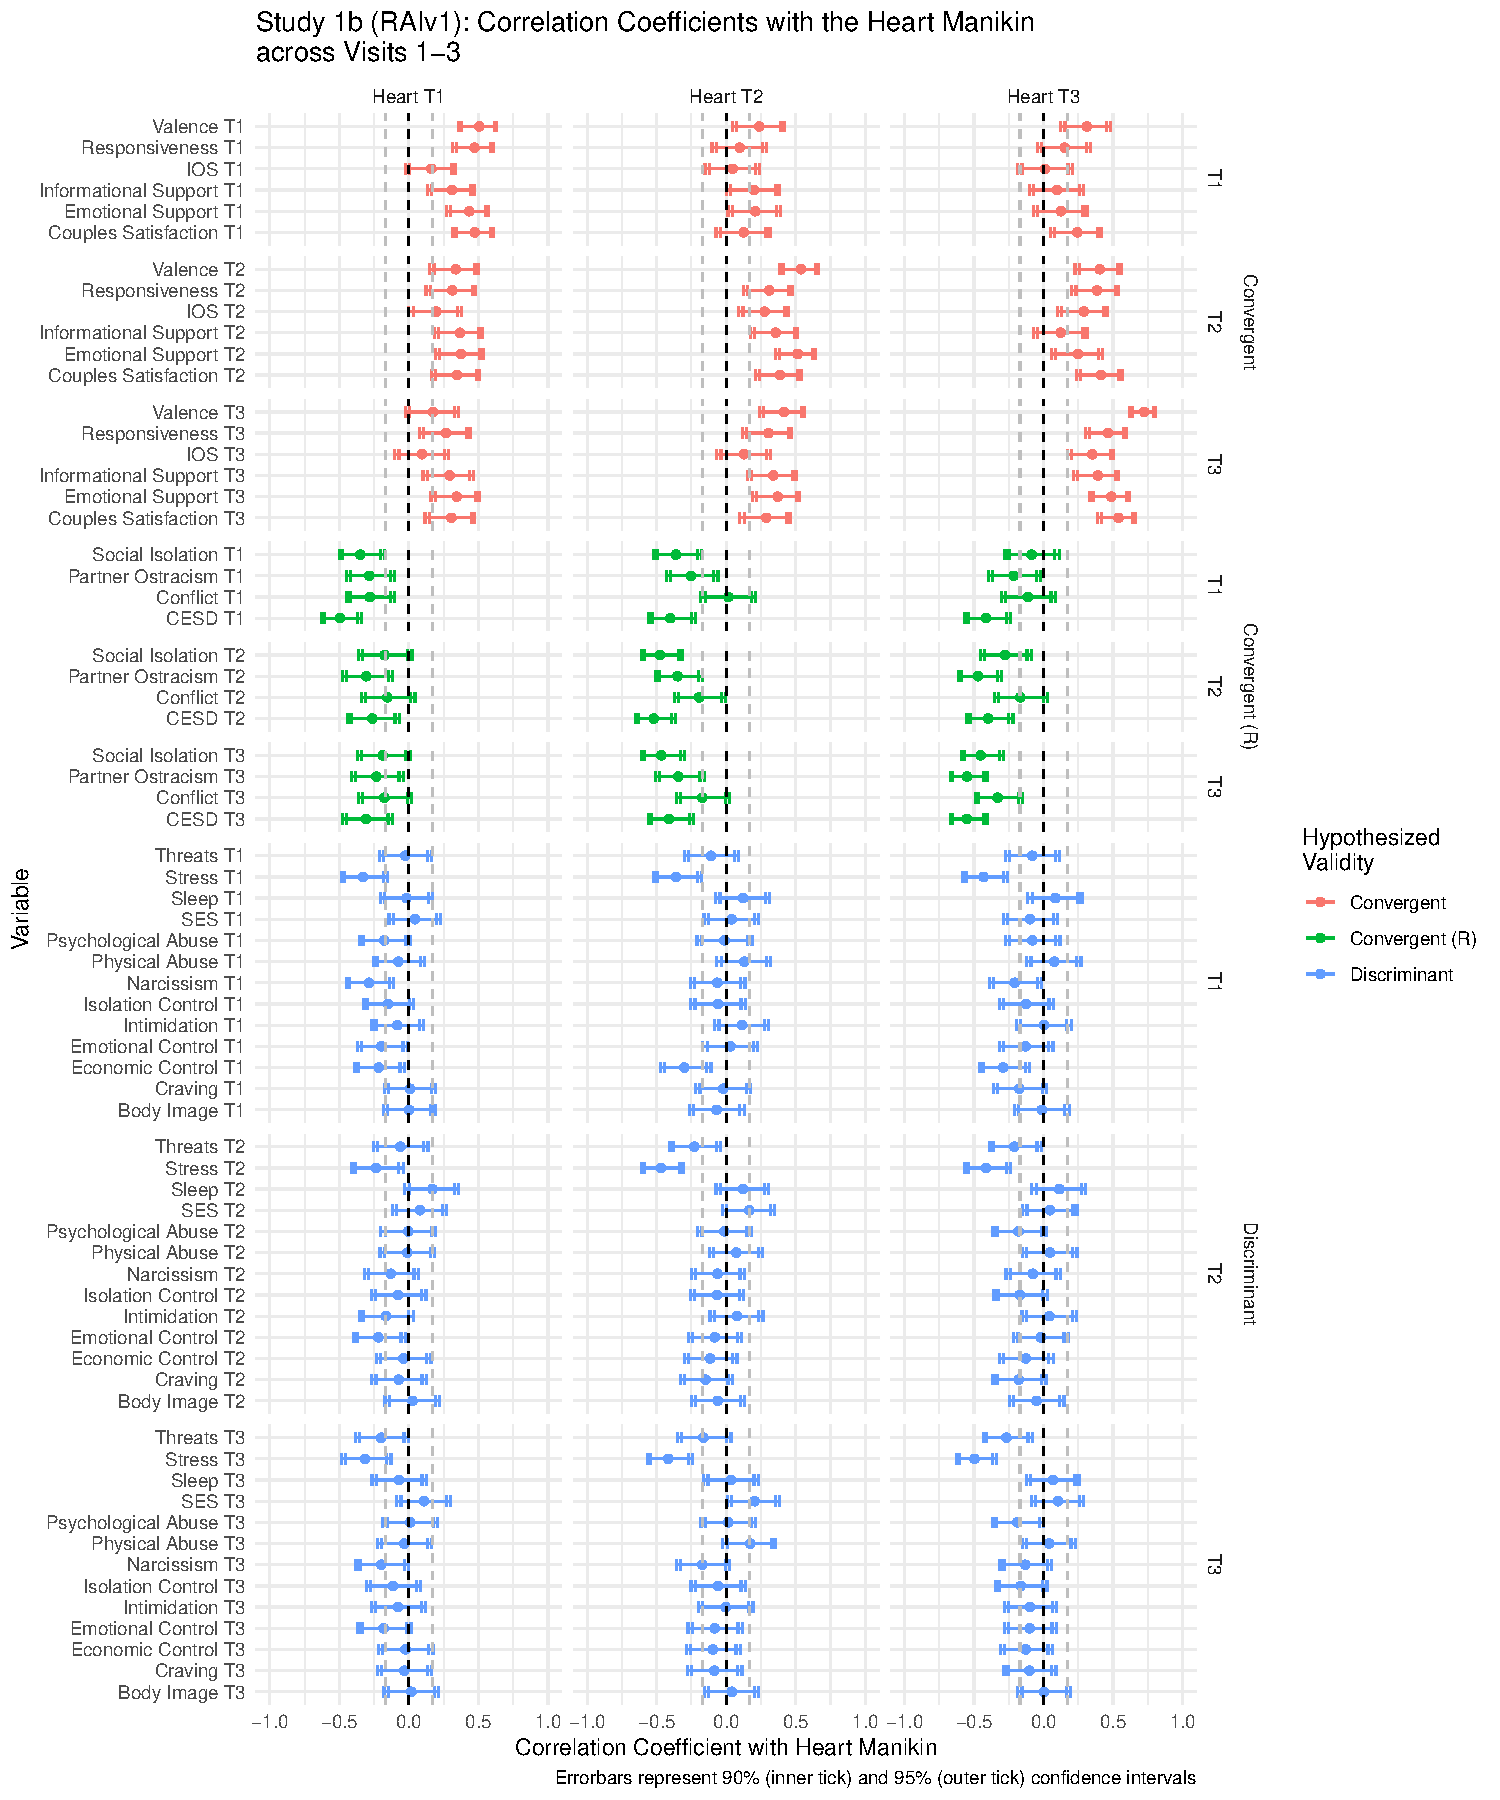
\includegraphics[keepaspectratio]{Sunami-Dissertation_files/figure-latex/appendix-s1b-forest-1.pdf}}
\caption{\label{fig:appendix-s1b-forest}Study 1b (RAIv1) - Forest plot of correlation coefficients of the measured variables with the Heart Manikin Scores}
\end{figure}

\subsection{Study 1c (ARv1)}\label{study-1c-arv1-2}

\begin{landscape}\begin{table}
\centering
\caption{\label{tab:appendix-s1c-correlations-table}Study 1c - Descriptive Statistics and Correlations among Variables}
\centering
\begin{threeparttable}
\resizebox{\ifdim\width>\linewidth\linewidth\else\width\fi}{!}{
\begin{tabular}[t]{>{\raggedright\arraybackslash}p{1.5in}cccccccccccccccc}
\toprule
\multicolumn{1}{c}{Variable} & \multicolumn{1}{c}{$n$} & \multicolumn{1}{c}{$M$} & \multicolumn{1}{c}{$SD$} & \multicolumn{1}{c}{1} & \multicolumn{1}{c}{2} & \multicolumn{1}{c}{3} & \multicolumn{1}{c}{4} & \multicolumn{1}{c}{5} & \multicolumn{1}{c}{6} & \multicolumn{1}{c}{7} & \multicolumn{1}{c}{8} & \multicolumn{1}{c}{9} & \multicolumn{1}{c}{10} & \multicolumn{1}{c}{11} & \multicolumn{1}{c}{12} & \multicolumn{1}{c}{13}\\
\midrule
1. Heart T1 & 290 & 6.69 & 1.81 &  &  &  &  &  &  &  &  &  &  &  &  & \\
2. Heart T2 & 290 & 5.11 & 2.96 & .12* &  &  &  &  &  &  &  &  &  &  &  & \\
3. Heart T3 & 290 & 6.64 & 2.39 & .66* & .48* &  &  &  &  &  &  &  &  &  &  & \\
4. Valence T1 & 290 & 6.58 & 1.79 & .70* & .11 & .52* &  &  &  &  &  &  &  &  &  & \\
5. Valence T2 & 290 & 5.08 & 2.84 & .13* & .92* & .46* & .16* &  &  &  &  &  &  &  &  & \\
\addlinespace
6. Valence T3 & 290 & 7.00 & 2.64 & .51* & .42* & .73* & .53* & .43* &  &  &  &  &  &  &  & \\
7. Arousal T2 & 290 & 5.47 & 2.07 & .07 & .33* & .26* & .00 & .34* & .25* &  &  &  &  &  &  & \\
8. Dominance T2 & 290 & 4.92 & 2.26 & .05 & .80* & .37* & .09 & .75* & .34* & .30* &  &  &  &  &  & \\
9. NTS Belonging T2 & 290 & 55.05 & 35.12 & .02 & .85* & .35* & -.01 & .85* & .31* & .28* & .68* &  &  &  &  & \\
10. NTS Self-Esteem T2 & 290 & 53.24 & 31.42 & .08 & .80* & .37* & .08 & .80* & .36* & .25* & .71* & .84* &  &  &  & \\
\addlinespace
11. NTS Control T2 & 290 & 39.24 & 26.52 & .06 & .64* & .33* & .09 & .63* & .28* & .21* & .68* & .58* & .71* &  &  & \\
12. NTS Meaning T2 & 290 & 57.72 & 30.77 & .00 & .78* & .30* & -.03 & .75* & .29* & .29* & .65* & .87* & .83* & .60* &  & \\
13. NTS Overall T2 & 290 & 51.60 & 28.33 & .04 & .86* & .37* & .03 & .85* & .34* & .29* & .75* & .94* & .94* & .77* & .93* & \\
14. SES T3 & 290 & 48.90 & 19.08 & .27* & .12* & .18* & .22* & .09 & .14* & .03 & .15* & .06 & .11 & .11 & .02 & .08\\
\bottomrule
\end{tabular}}
\begin{tablenotes}[para]
\item \textit{Note.} 
\item Heart = the Heart Manikin, SES = Subjective Socioeconomic Status, IOS = Inclusion of the Other in the Self Scale, NTS = the Need-Threat Scale
\end{tablenotes}
\end{threeparttable}
\end{table}
\end{landscape}

\begin{figure}
\centering
\pandocbounded{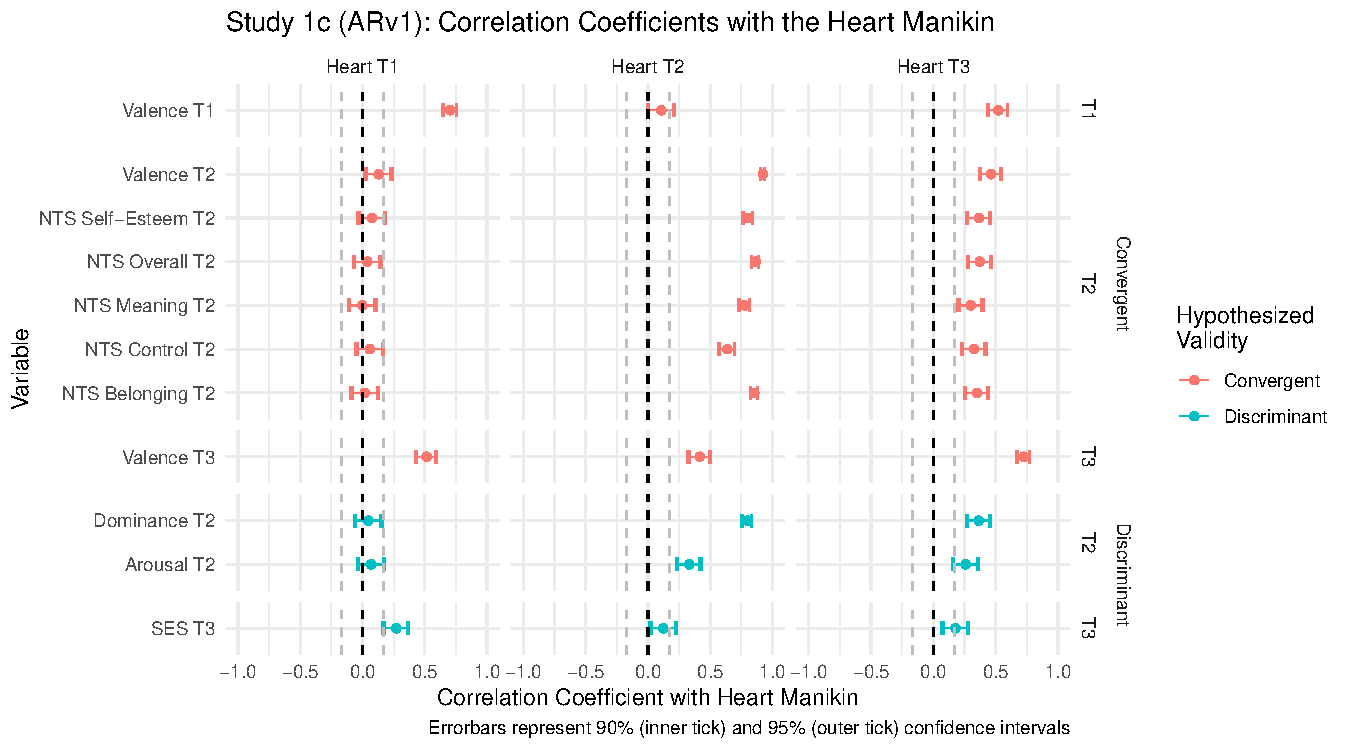
\includegraphics[keepaspectratio]{Sunami-Dissertation_files/figure-latex/appendix-s1c-all-cors-plot-1.pdf}}
\caption{\label{fig:appendix-s1c-all-cors-plot}Study 1c - Forestplot of Correlation Coefficients between the Measured Variabels with the Heart Manikin}
\end{figure}

I explored whether the heart manikin scores changed across time by condition in a mixed model.

\begin{figure}
\centering
\pandocbounded{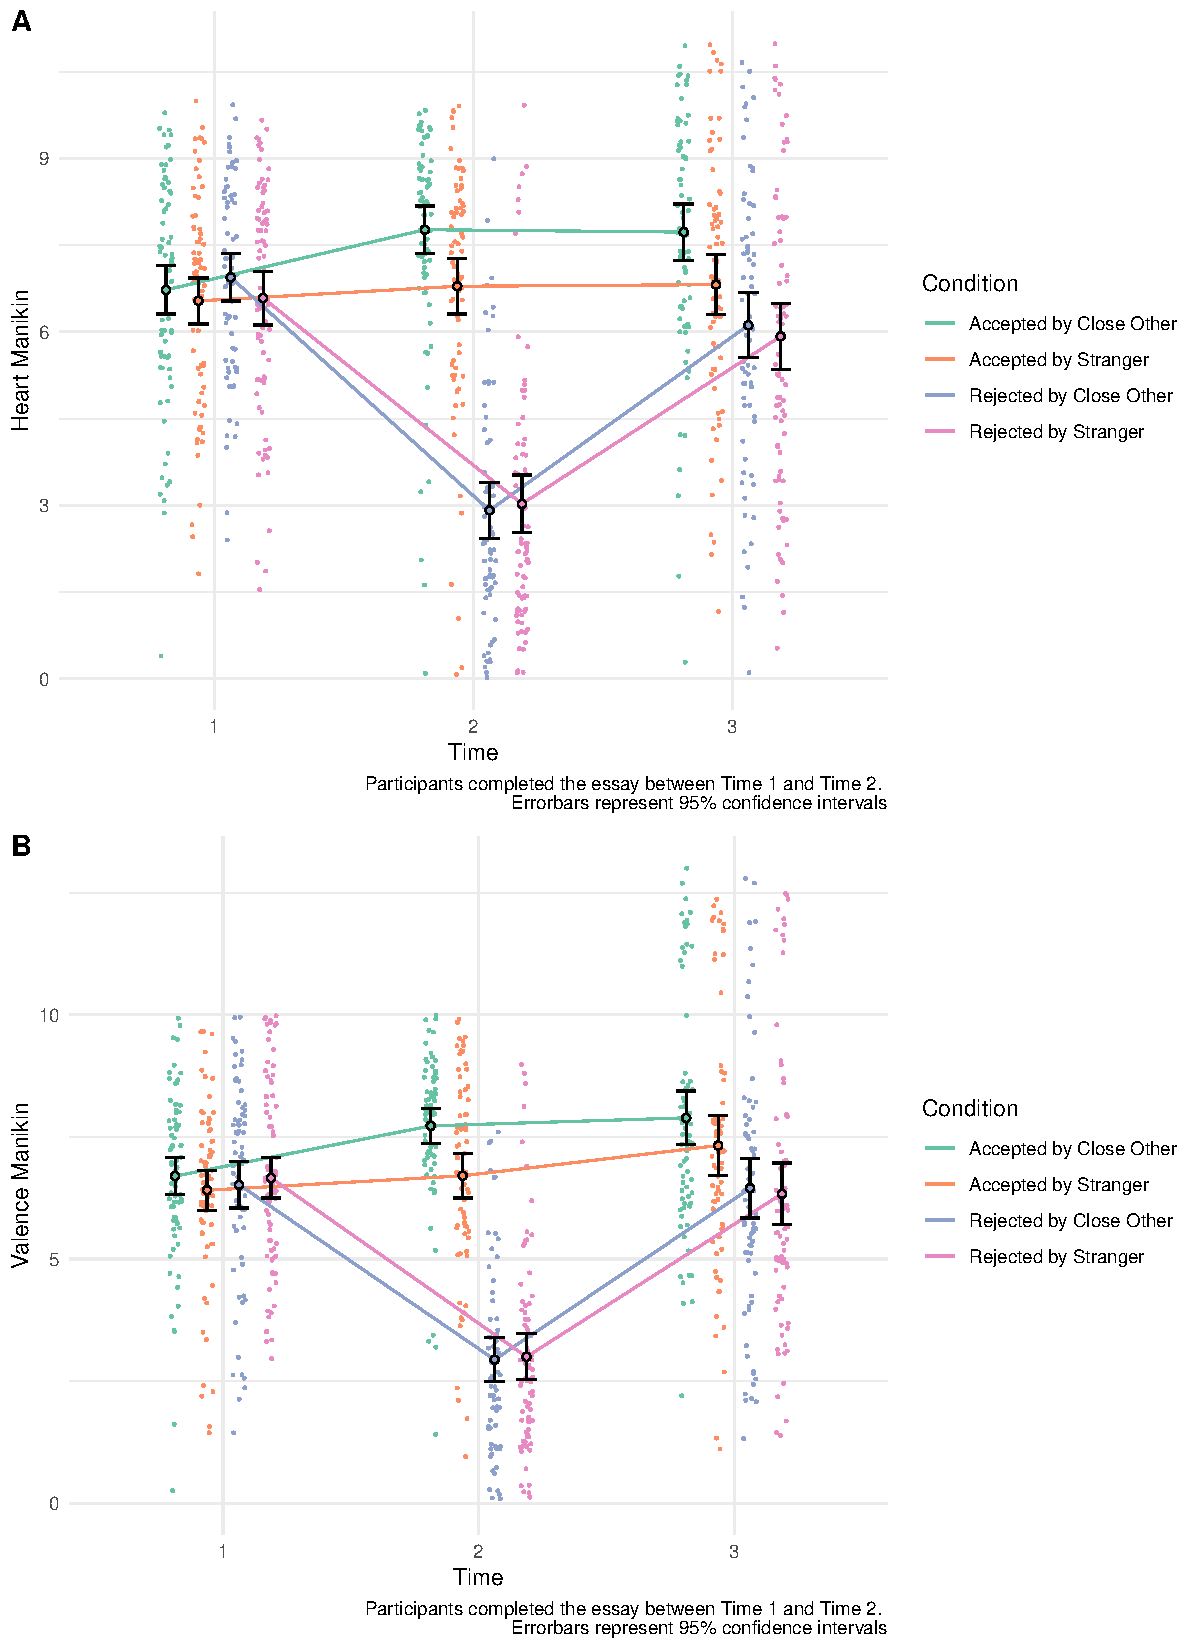
\includegraphics[keepaspectratio]{Sunami-Dissertation_files/figure-latex/appnedix-s1c-belonging-across-time-1.pdf}}
\caption{\label{fig:appnedix-s1c-belonging-across-time}Study 1c - Heart Manikin Scores Across Time and Conditions}
\end{figure}

\subsection{Study 1d (EVv1)}\label{study-1d-evv1-2}

\begin{landscape}\begin{table}
\centering
\caption{\label{tab:appendix-s1d-correlations-table}Study 1d - Descriptive Statistics and Correlations among Variables}
\centering
\resizebox{\ifdim\width>\linewidth\linewidth\else\width\fi}{!}{
\begin{tabular}[t]{>{\raggedright\arraybackslash}p{1.2in}ccccccccccccccccccccccccccccccc}
\toprule
\multicolumn{1}{c}{Variable} & \multicolumn{1}{c}{$n$} & \multicolumn{1}{c}{$M$} & \multicolumn{1}{c}{$SD$} & \multicolumn{1}{c}{1} & \multicolumn{1}{c}{2} & \multicolumn{1}{c}{3} & \multicolumn{1}{c}{4} & \multicolumn{1}{c}{5} & \multicolumn{1}{c}{6} & \multicolumn{1}{c}{7} & \multicolumn{1}{c}{8} & \multicolumn{1}{c}{9} & \multicolumn{1}{c}{10} & \multicolumn{1}{c}{11} & \multicolumn{1}{c}{12} & \multicolumn{1}{c}{13} & \multicolumn{1}{c}{14} & \multicolumn{1}{c}{15} & \multicolumn{1}{c}{16} & \multicolumn{1}{c}{17} & \multicolumn{1}{c}{18} & \multicolumn{1}{c}{19} & \multicolumn{1}{c}{20} & \multicolumn{1}{c}{21} & \multicolumn{1}{c}{22} & \multicolumn{1}{c}{23} & \multicolumn{1}{c}{24} & \multicolumn{1}{c}{25} & \multicolumn{1}{c}{26} & \multicolumn{1}{c}{27} & \multicolumn{1}{c}{28}\\
\midrule
1. Heart T1 & 242 & 6.57 & 1.79 &  &  &  &  &  &  &  &  &  &  &  &  &  &  &  &  &  &  &  &  &  &  &  &  &  &  &  & \\
2. Heart T2 & 242 & 6.63 & 1.60 & .84* &  &  &  &  &  &  &  &  &  &  &  &  &  &  &  &  &  &  &  &  &  &  &  &  &  &  & \\
3. Heart T3 & 238 & 6.34 & 1.81 & .59* & .66* &  &  &  &  &  &  &  &  &  &  &  &  &  &  &  &  &  &  &  &  &  &  &  &  &  & \\
4. Heart T4 & 237 & 6.37 & 1.64 & .70* & .80* & .74* &  &  &  &  &  &  &  &  &  &  &  &  &  &  &  &  &  &  &  &  &  &  &  &  & \\
5. Valence T1 & 242 & 6.66 & 1.35 & .47* & .44* & .35* & .39* &  &  &  &  &  &  &  &  &  &  &  &  &  &  &  &  &  &  &  &  &  &  &  & \\
\addlinespace
6. Valence T2 & 242 & 6.45 & 1.39 & .22* & .41* & .15* & .27* & .59* &  &  &  &  &  &  &  &  &  &  &  &  &  &  &  &  &  &  &  &  &  &  & \\
7. Valence T3 & 238 & 6.03 & 1.78 & .25* & .27* & .65* & .37* & .46* & .34* &  &  &  &  &  &  &  &  &  &  &  &  &  &  &  &  &  &  &  &  &  & \\
8. Valence T4 & 237 & 5.93 & 1.61 & .39* & .47* & .49* & .56* & .61* & .49* & .61* &  &  &  &  &  &  &  &  &  &  &  &  &  &  &  &  &  &  &  &  & \\
9. Arousal T1 & 242 & 4.05 & 1.48 & .09 & .12 & .04 & .07 & .24* & .25* & .25* & .25* &  &  &  &  &  &  &  &  &  &  &  &  &  &  &  &  &  &  &  & \\
10. Arousal T2 & 242 & 4.74 & 1.64 & .02 & .11 & -.05 & -.01 & .28* & .37* & .15* & .21* & .66* &  &  &  &  &  &  &  &  &  &  &  &  &  &  &  &  &  &  & \\
\addlinespace
11. Arousal T3 & 238 & 4.74 & 1.74 & .01 & .04 & .17* & .05 & .21* & .17* & .38* & .30* & .59* & .72* &  &  &  &  &  &  &  &  &  &  &  &  &  &  &  &  &  & \\
12. Arousal T4 & 237 & 4.79 & 1.71 & .13 & .18* & .09 & .12 & .26* & .30* & .27* & .34* & .61* & .73* & .74* &  &  &  &  &  &  &  &  &  &  &  &  &  &  &  &  & \\
13. Dominance T1 & 242 & 6.23 & 1.50 & .31* & .31* & .23* & .34* & .30* & .23* & .17* & .35* & .07 & .11 & .12 & .14* &  &  &  &  &  &  &  &  &  &  &  &  &  &  &  & \\
14. Dominance T2 & 242 & 6.34 & 1.42 & .26* & .43* & .31* & .41* & .31* & .35* & .21* & .36* & .08 & .16* & .09 & .16* & .75* &  &  &  &  &  &  &  &  &  &  &  &  &  &  & \\
15. Dominance T3 & 238 & 6.21 & 1.53 & .16* & .29* & .51* & .44* & .24* & .25* & .49* & .43* & .04 & .04 & .18* & .13* & .62* & .69* &  &  &  &  &  &  &  &  &  &  &  &  &  & \\
\addlinespace
16. Dominance T4 & 237 & 6.23 & 1.51 & .27* & .37* & .40* & .54* & .30* & .20* & .33* & .55* & .06 & .05 & .08 & .14* & .61* & .71* & .67* &  &  &  &  &  &  &  &  &  &  &  &  & \\
17. Self-Esteem T1 & 241 & 1.54 & 0.96 & .57* & .57* & .43* & .49* & .41* & .32* & .30* & .35* & .03 & .05 & .03 & .06 & .30* & .34* & .31* & .34* &  &  &  &  &  &  &  &  &  &  &  & \\
18. Need for Closure T1 & 238 & 0.33 & 0.76 & -.06 & -.07 & -.08 & -.04 & .03 & -.02 & -.08 & .01 & .02 & .12 & .08 & .09 & -.07 & -.04 & -.07 & -.09 & -.19* &  &  &  &  &  &  &  &  &  &  & \\
19. NTS Belonging T3 & 238 & 72.51 & 20.50 & .23* & .26* & .63* & .36* & .18* & -.01 & .57* & .27* & .00 & -.08 & .19* & .03 & .13* & .18* & .41* & .21* & .28* & -.18* &  &  &  &  &  &  &  &  &  & \\
20. NTS Self-Esteem T3 & 238 & 69.90 & 19.48 & .28* & .31* & .61* & .43* & .28* & .09 & .61* & .37* & .09 & -.05 & .19* & .08 & .21* & .26* & .49* & .40* & .49* & -.20* & .71* &  &  &  &  &  &  &  &  & \\
\addlinespace
21. NTS Control T3 & 238 & 49.46 & 21.11 & .06 & .13* & .31* & .23* & .13* & .11 & .35* & .30* & .04 & .02 & .17* & .08 & .16* & .27* & .42* & .34* & .27* & -.14* & .48* & .54* &  &  &  &  &  &  &  & \\
22. NTS Meaning T3 & 238 & 76.45 & 18.00 & .33* & .33* & .64* & .41* & .28* & .06 & .59* & .31* & .10 & -.01 & .23* & .10 & .15* & .19* & .43* & .29* & .45* & -.15* & .76* & .79* & .45* &  &  &  &  &  &  & \\
23. NTS Overall T3 & 238 & 65.27 & 16.65 & .25* & .30* & .60* & .41* & .27* & .11 & .60* & .39* & .09 & -.02 & .23* & .10 & .20* & .28* & .52* & .40* & .47* & -.19* & .75* & .90* & .80* & .86* &  &  &  &  &  & \\
24. NTS Belonging T4 & 237 & 75.65 & 16.70 & .31* & .38* & .55* & .54* & .24* & .10 & .41* & .41* & .07 & -.07 & .08 & .03 & .17* & .25* & .40* & .43* & .43* & -.20* & .61* & .62* & .37* & .63* & .62* &  &  &  &  & \\
25. NTS Self-Esteem T4 & 237 & 66.59 & 20.17 & .28* & .42* & .41* & .52* & .28* & .23* & .26* & .46* & .06 & -.04 & .01 & .04 & .22* & .31* & .36* & .54* & .47* & -.15* & .28* & .55* & .35* & .38* & .50* & .67* &  &  &  & \\
\addlinespace
26. NTS Control T4 & 237 & 51.86 & 22.80 & .18* & .28* & .26* & .37* & .25* & .19* & .14* & .35* & .09 & .03 & .06 & .04 & .24* & .31* & .31* & .45* & .37* & -.16* & .19* & .40* & .57* & .27* & .49* & .44* & .65* &  &  & \\
27. NTS Meaning T4 & 237 & 77.25 & 16.49 & .30* & .40* & .51* & .53* & .22* & .11 & .39* & .43* & .09 & -.01 & .10 & .08 & .19* & .29* & .40* & .50* & .46* & -.12 & .46* & .57* & .35* & .58* & .58* & .80* & .72* & .48* &  & \\
28. NTS Overall T4 & 237 & 68.44 & 15.95 & .31* & .43* & .50* & .58* & .29* & .19* & .35* & .48* & .09 & -.03 & .07 & .05 & .24* & .34* & .43* & .56* & .51* & -.19* & .45* & .63* & .49* & .54* & .65* & .85* & .89* & .78* & .87* & \\
29. Social Judgement Survey T4 & 237 & 418.70 & 226.03 & .01 & -.07 & .00 & -.05 & .00 & -.08 & -.04 & -.01 & -.15* & -.12 & -.09 & -.06 & .13* & .11 & .04 & .11 & .00 & .07 & .01 & -.01 & -.01 & -.06 & -.03 & -.03 & .01 & .01 & -.02 & -.01\\
\bottomrule
\multicolumn{32}{l}{\rule{0pt}{1em}\textit{Note.} Heart = the Heart Manikin, NTS = the Need-Threat Scale}\\
\end{tabular}}
\end{table}
\end{landscape}

\begin{figure}
\centering
\pandocbounded{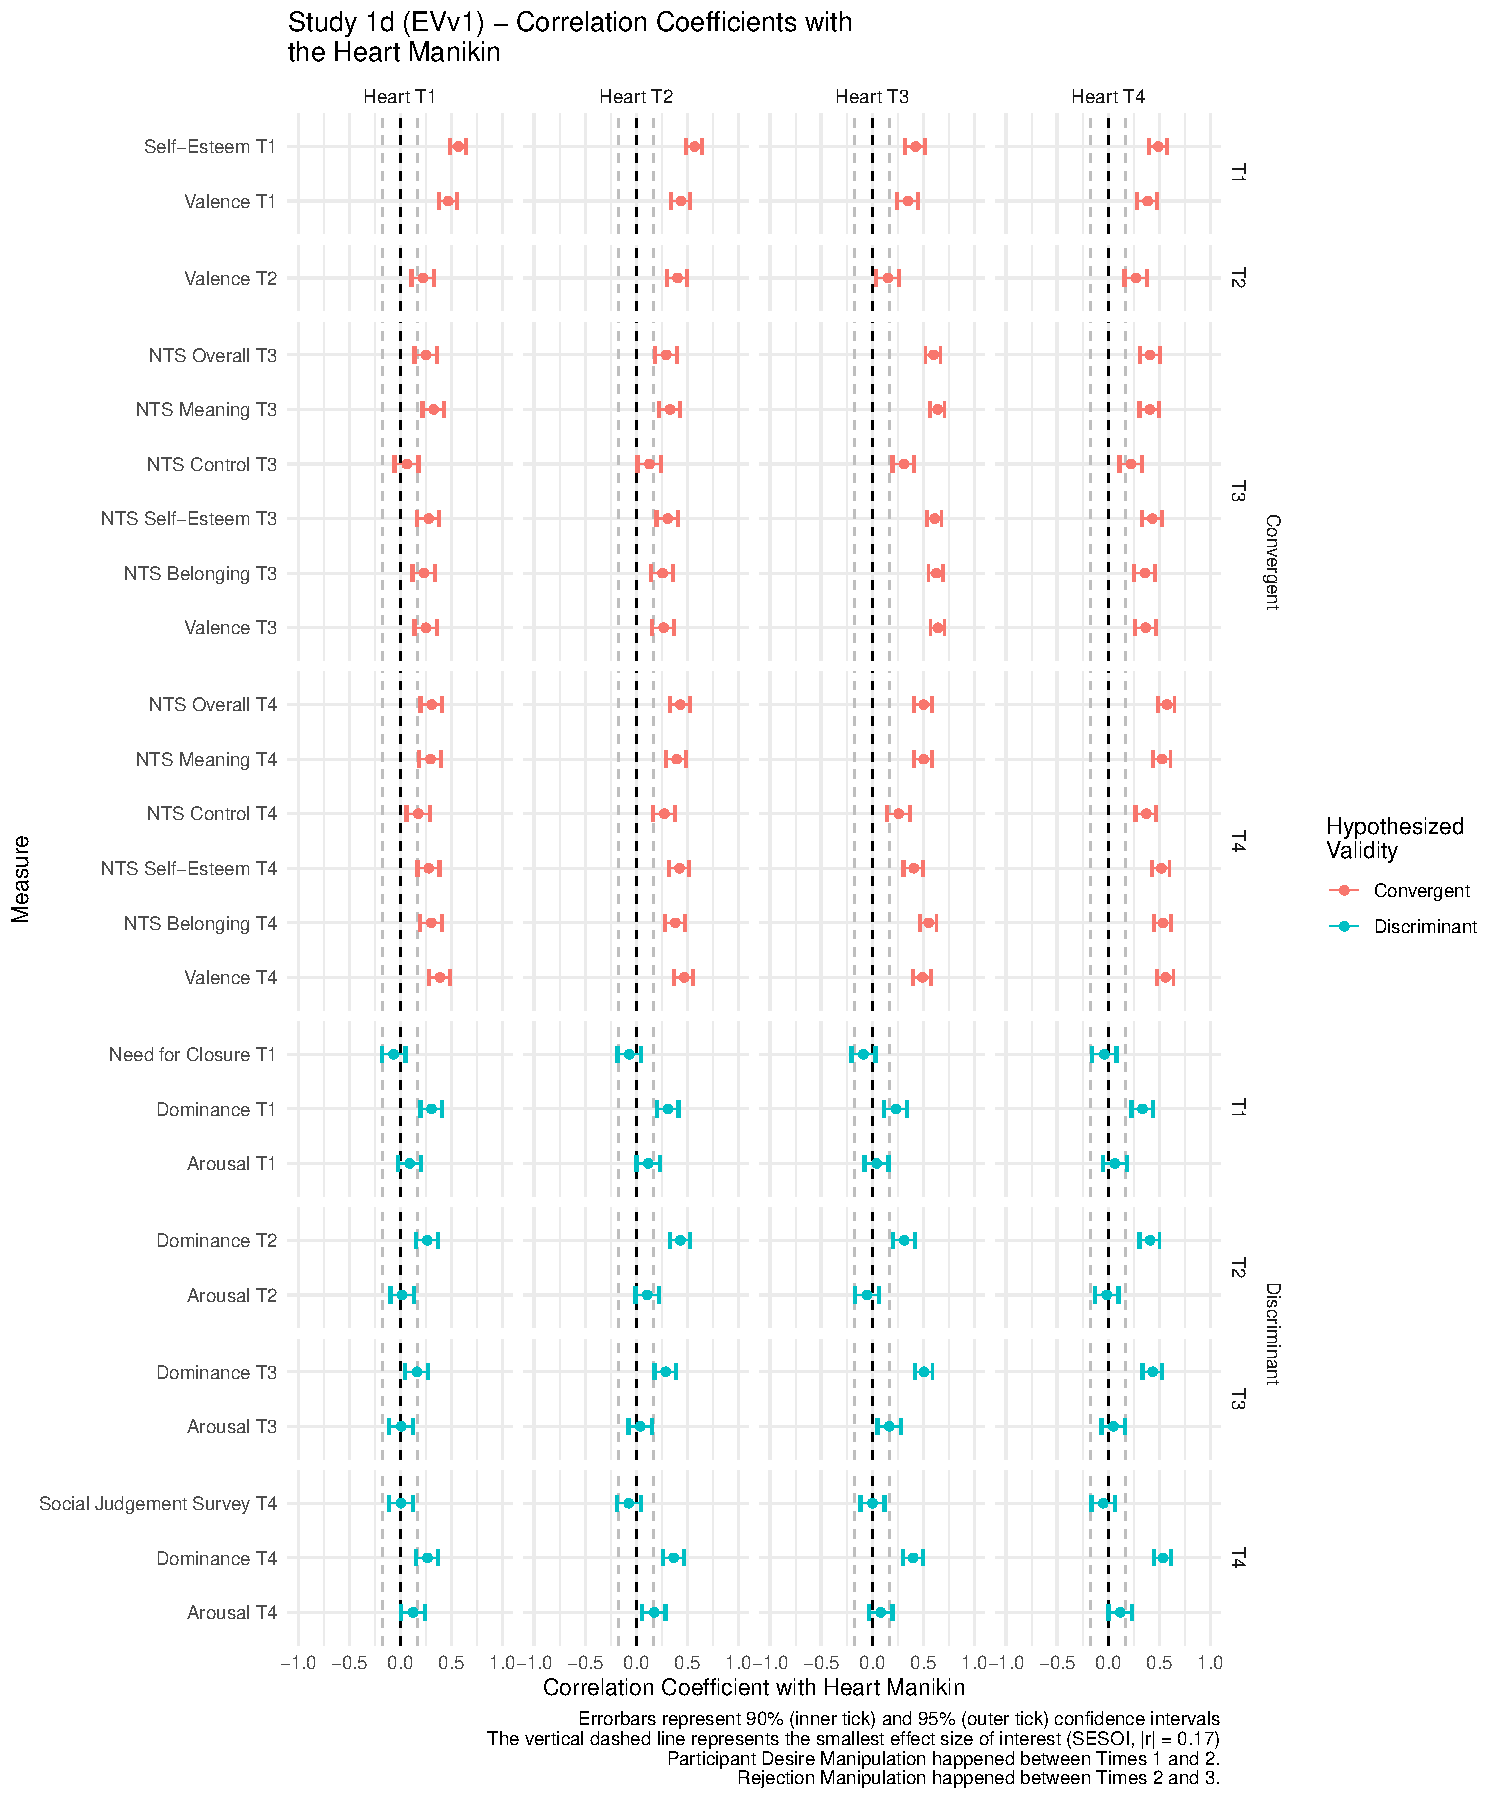
\includegraphics[keepaspectratio]{Sunami-Dissertation_files/figure-latex/appendix-s1d-all-forestplot-1.pdf}}
\caption{\label{fig:appendix-s1d-all-forestplot}Study 1d - Forestplot of Correlation Coefficients between the Measured Scores and the Heart Manikin}
\end{figure}

\begin{figure}
\centering
\pandocbounded{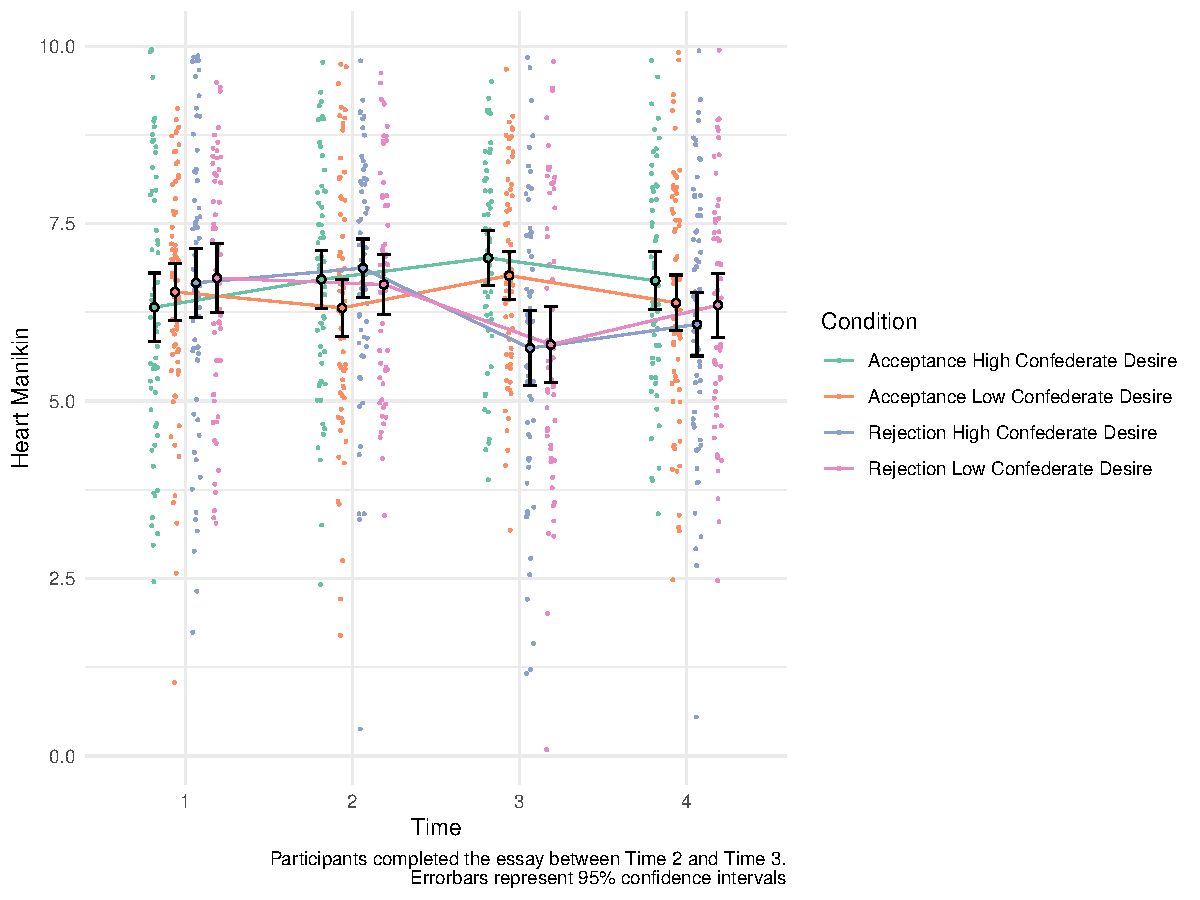
\includegraphics[keepaspectratio]{Sunami-Dissertation_files/figure-latex/appendix-s1d-sensitivity-plot-1.pdf}}
\caption{\label{fig:appendix-s1d-sensitivity-plot}Study 1d - Heart Manikin Across Time}
\end{figure}

\subsection{Study 1e (NPSv2)}\label{study-1e-npsv2-2}

\begin{landscape}\begin{table}
\centering
\caption{\label{tab:appendix-s1e-correlations-table}Study 1e - Descriptive Statistics and Correlation Coefficients}
\centering
\resizebox{\ifdim\width>\linewidth\linewidth\else\width\fi}{!}{
\begin{tabular}[t]{>{\raggedright\arraybackslash}p{1.2in}cccccccccccccccccccccccccccccccccccccccccc}
\toprule
\multicolumn{1}{c}{Variable} & \multicolumn{1}{c}{$n$} & \multicolumn{1}{c}{$M$} & \multicolumn{1}{c}{$SD$} & \multicolumn{1}{c}{1} & \multicolumn{1}{c}{2} & \multicolumn{1}{c}{3} & \multicolumn{1}{c}{4} & \multicolumn{1}{c}{5} & \multicolumn{1}{c}{6} & \multicolumn{1}{c}{7} & \multicolumn{1}{c}{8} & \multicolumn{1}{c}{9} & \multicolumn{1}{c}{10} & \multicolumn{1}{c}{11} & \multicolumn{1}{c}{12} & \multicolumn{1}{c}{13} & \multicolumn{1}{c}{14} & \multicolumn{1}{c}{15} & \multicolumn{1}{c}{16} & \multicolumn{1}{c}{17} & \multicolumn{1}{c}{18} & \multicolumn{1}{c}{19} & \multicolumn{1}{c}{20} & \multicolumn{1}{c}{21} & \multicolumn{1}{c}{22} & \multicolumn{1}{c}{23} & \multicolumn{1}{c}{24} & \multicolumn{1}{c}{25} & \multicolumn{1}{c}{26} & \multicolumn{1}{c}{27} & \multicolumn{1}{c}{28} & \multicolumn{1}{c}{29} & \multicolumn{1}{c}{30} & \multicolumn{1}{c}{31} & \multicolumn{1}{c}{32} & \multicolumn{1}{c}{33} & \multicolumn{1}{c}{34} & \multicolumn{1}{c}{35} & \multicolumn{1}{c}{36} & \multicolumn{1}{c}{37} & \multicolumn{1}{c}{38} & \multicolumn{1}{c}{39}\\
\midrule
1. Heart T1 & 538 & 6.96 & 1.62 &  &  &  &  &  &  &  &  &  &  &  &  &  &  &  &  &  &  &  &  &  &  &  &  &  &  &  &  &  &  &  &  &  &  &  &  &  &  & \\
2. Heart T2 & 538 & 7.00 & 1.49 & .83* &  &  &  &  &  &  &  &  &  &  &  &  &  &  &  &  &  &  &  &  &  &  &  &  &  &  &  &  &  &  &  &  &  &  &  &  &  & \\
3. Heart T3 & 538 & 6.89 & 1.55 & .71* & .84* &  &  &  &  &  &  &  &  &  &  &  &  &  &  &  &  &  &  &  &  &  &  &  &  &  &  &  &  &  &  &  &  &  &  &  &  & \\
4. Heart T4 & 538 & 6.83 & 1.58 & .63* & .69* & .63* &  &  &  &  &  &  &  &  &  &  &  &  &  &  &  &  &  &  &  &  &  &  &  &  &  &  &  &  &  &  &  &  &  &  &  & \\
5. Heart T5 & 538 & 6.63 & 1.73 & .61* & .65* & .59* & .85* &  &  &  &  &  &  &  &  &  &  &  &  &  &  &  &  &  &  &  &  &  &  &  &  &  &  &  &  &  &  &  &  &  &  & \\
\addlinespace
6. Heart T6 & 538 & 6.81 & 1.56 & .65* & .71* & .66* & .87* & .87* &  &  &  &  &  &  &  &  &  &  &  &  &  &  &  &  &  &  &  &  &  &  &  &  &  &  &  &  &  &  &  &  &  & \\
7. Valence T1 & 538 & 6.40 & 1.51 & .52* & .49* & .42* & .40* & .39* & .43* &  &  &  &  &  &  &  &  &  &  &  &  &  &  &  &  &  &  &  &  &  &  &  &  &  &  &  &  &  &  &  &  & \\
8. Valence T2 & 538 & 6.39 & 1.45 & .46* & .51* & .43* & .42* & .36* & .43* & .71* &  &  &  &  &  &  &  &  &  &  &  &  &  &  &  &  &  &  &  &  &  &  &  &  &  &  &  &  &  &  &  & \\
9. Valence T3 & 538 & 6.48 & 1.64 & .42* & .45* & .59* & .41* & .35* & .43* & .55* & .68* &  &  &  &  &  &  &  &  &  &  &  &  &  &  &  &  &  &  &  &  &  &  &  &  &  &  &  &  &  &  & \\
10. Valence T4 & 538 & 6.16 & 1.56 & .40* & .44* & .43* & .54* & .50* & .53* & .49* & .53* & .54* &  &  &  &  &  &  &  &  &  &  &  &  &  &  &  &  &  &  &  &  &  &  &  &  &  &  &  &  &  & \\
\addlinespace
11. Valence T5 & 538 & 5.89 & 1.67 & .42* & .43* & .39* & .57* & .65* & .57* & .46* & .48* & .45* & .82* &  &  &  &  &  &  &  &  &  &  &  &  &  &  &  &  &  &  &  &  &  &  &  &  &  &  &  &  & \\
12. Valence T6 & 538 & 6.19 & 1.61 & .42* & .46* & .43* & .55* & .55* & .59* & .49* & .55* & .51* & .82* & .82* &  &  &  &  &  &  &  &  &  &  &  &  &  &  &  &  &  &  &  &  &  &  &  &  &  &  &  & \\
13. Arousal T1 & 538 & 4.37 & 1.46 & .16* & .16* & .11* & .11* & .10* & .14* & .27* & .26* & .24* & .18* & .17* & .20* &  &  &  &  &  &  &  &  &  &  &  &  &  &  &  &  &  &  &  &  &  &  &  &  &  &  & \\
14. Arousal T2 & 538 & 4.65 & 1.56 & .12* & .13* & .07 & .10* & .07 & .10* & .19* & .34* & .23* & .15* & .15* & .18* & .72* &  &  &  &  &  &  &  &  &  &  &  &  &  &  &  &  &  &  &  &  &  &  &  &  &  & \\
15. Arousal T3 & 538 & 4.90 & 1.62 & .12* & .11* & .15* & .10* & .07 & .11* & .16* & .27* & .33* & .19* & .16* & .19* & .66* & .85* &  &  &  &  &  &  &  &  &  &  &  &  &  &  &  &  &  &  &  &  &  &  &  &  & \\
\addlinespace
16. Arousal T4 & 538 & 4.56 & 1.60 & .08 & .13* & .12* & .17* & .15* & .13* & .13* & .18* & .21* & .35* & .28* & .26* & .44* & .48* & .49* &  &  &  &  &  &  &  &  &  &  &  &  &  &  &  &  &  &  &  &  &  &  &  & \\
17. Arousal T5 & 538 & 4.59 & 1.59 & .11* & .15* & .10* & .15* & .16* & .16* & .14* & .19* & .17* & .28* & .31* & .27* & .45* & .49* & .50* & .85* &  &  &  &  &  &  &  &  &  &  &  &  &  &  &  &  &  &  &  &  &  &  & \\
18. Arousal T6 & 538 & 4.78 & 1.63 & .07 & .12* & .08 & .13* & .14* & .17* & .11* & .20* & .19* & .30* & .30* & .32* & .45* & .49* & .51* & .83* & .88* &  &  &  &  &  &  &  &  &  &  &  &  &  &  &  &  &  &  &  &  &  & \\
19. Dominance T1 & 538 & 6.25 & 1.40 & .34* & .33* & .27* & .26* & .28* & .29* & .27* & .25* & .27* & .15* & .20* & .22* & .12* & .12* & .08 & .06 & .07 & .07 &  &  &  &  &  &  &  &  &  &  &  &  &  &  &  &  &  &  &  &  & \\
20. Dominance T2 & 538 & 6.36 & 1.37 & .33* & .39* & .36* & .30* & .32* & .33* & .28* & .32* & .34* & .25* & .26* & .29* & .12* & .13* & .09* & .07 & .08 & .08 & .78* &  &  &  &  &  &  &  &  &  &  &  &  &  &  &  &  &  &  &  & \\
\addlinespace
21. Dominance T3 & 538 & 6.38 & 1.39 & .33* & .38* & .43* & .31* & .32* & .34* & .29* & .33* & .46* & .29* & .30* & .32* & .14* & .14* & .14* & .08 & .06 & .08 & .71* & .89* &  &  &  &  &  &  &  &  &  &  &  &  &  &  &  &  &  &  & \\
22. Dominance T4 & 538 & 6.38 & 1.37 & .34* & .38* & .34* & .48* & .45* & .44* & .23* & .30* & .33* & .41* & .43* & .39* & .11* & .07 & .08 & .16* & .14* & .13* & .54* & .64* & .64* &  &  &  &  &  &  &  &  &  &  &  &  &  &  &  &  &  & \\
23. Dominance T5 & 538 & 6.21 & 1.46 & .37* & .40* & .37* & .45* & .57* & .50* & .27* & .31* & .31* & .36* & .50* & .41* & .08 & .08 & .07 & .11* & .14* & .11* & .54* & .66* & .66* & .82* &  &  &  &  &  &  &  &  &  &  &  &  &  &  &  &  & \\
24. Dominance T6 & 538 & 6.35 & 1.41 & .37* & .41* & .38* & .46* & .49* & .54* & .30* & .33* & .33* & .39* & .44* & .44* & .10* & .09* & .08 & .06 & .10* & .12* & .56* & .65* & .66* & .80* & .83* &  &  &  &  &  &  &  &  &  &  &  &  &  &  &  & \\
25. Attachment Avoidance T1 & 510 & -0.94 & 1.05 & -.41* & -.42* & -.36* & -.37* & -.40* & -.39* & -.23* & -.20* & -.22* & -.17* & -.19* & -.20* & -.11* & -.05 & -.06 & -.10* & -.09* & -.06 & -.15* & -.17* & -.18* & -.25* & -.25* & -.21* &  &  &  &  &  &  &  &  &  &  &  &  &  &  & \\
\addlinespace
26. Attachment Anxiety T1 & 510 & -0.38 & 1.09 & -.41* & -.35* & -.32* & -.35* & -.37* & -.38* & -.27* & -.22* & -.20* & -.19* & -.24* & -.22* & -.06 & .05 & .08 & .08 & .07 & .08 & -.25* & -.26* & -.22* & -.24* & -.26* & -.28* & .18* &  &  &  &  &  &  &  &  &  &  &  &  &  & \\
27. Fear of Negative Evaluation T1 & 538 & 3.04 & 0.80 & -.30* & -.26* & -.25* & -.28* & -.30* & -.28* & -.19* & -.16* & -.14* & -.16* & -.21* & -.19* & -.01 & .06 & .09* & .07 & .08 & .08 & -.34* & -.35* & -.30* & -.30* & -.31* & -.29* & .14* & .48* &  &  &  &  &  &  &  &  &  &  &  &  & \\
28. Self-Esteem T1 & 538 & 1.44 & 1.02 & .52* & .49* & .43* & .49* & .47* & .50* & .45* & .34* & .30* & .30* & .35* & .36* & .13* & .08 & .06 & .03 & .05 & .02 & .38* & .35* & .33* & .36* & .41* & .38* & -.39* & -.53* & -.54* &  &  &  &  &  &  &  &  &  &  &  & \\
29. Subjective SES T1 & 538 & 66.04 & 13.19 & .05 & .05 & .04 & .01 & .03 & .04 & .09* & .06 & .02 & -.06 & -.03 & -.06 & .05 & .02 & .03 & -.02 & .00 & -.03 & .07 & -.01 & -.01 & -.03 & -.01 & .00 & -.10* & -.03 & .01 & .07 &  &  &  &  &  &  &  &  &  &  & \\
30. Rejection Sensitivity T1 & 538 & 7.12 & 2.96 & -.40* & -.39* & -.35* & -.36* & -.37* & -.36* & -.29* & -.16* & -.18* & -.26* & -.28* & -.24* & -.01 & .09* & .08 & .02 & .04 & .06 & -.24* & -.24* & -.23* & -.25* & -.28* & -.24* & .32* & .39* & .35* & -.41* & -.11* &  &  &  &  &  &  &  &  &  & \\
\addlinespace
31. NTS Belonging T3 & 535 & 81.60 & 15.38 & .43* & .44* & .55* & .45* & .43* & .47* & .33* & .29* & .44* & .34* & .32* & .33* & .04 & .05 & .10* & .10* & .05 & .07 & .27* & .29* & .32* & .26* & .32* & .29* & -.29* & -.30* & -.27* & .45* & .06 & -.31* &  &  &  &  &  &  &  &  & \\
32. NTS Belonging T5 & 536 & 80.58 & 15.54 & .49* & .46* & .45* & .57* & .66* & .58* & .32* & .28* & .29* & .34* & .47* & .40* & .02 & .02 & .03 & .03 & .05 & .06 & .32* & .33* & .30* & .36* & .49* & .41* & -.32* & -.40* & -.37* & .55* & .03 & -.34* & .69* &  &  &  &  &  &  &  & \\
33. NTS Self-Esteem T3 & 536 & 70.00 & 18.61 & .39* & .42* & .46* & .37* & .37* & .39* & .38* & .34* & .38* & .32* & .34* & .34* & .05 & .08 & .06 & .04 & .03 & .05 & .38* & .41* & .42* & .34* & .42* & .39* & -.22* & -.32* & -.44* & .59* & .06 & -.37* & .65* & .51* &  &  &  &  &  &  & \\
34. NTS Self-Esteem T5 & 538 & 68.26 & 19.22 & .40* & .37* & .32* & .48* & .58* & .50* & .32* & .27* & .20* & .31* & .47* & .40* & .08 & .08 & .03 & .01 & .05 & .05 & .39* & .40* & .36* & .41* & .53* & .46* & -.21* & -.42* & -.50* & .64* & .03 & -.34* & .42* & .69* & .62* &  &  &  &  &  & \\
35. NTS Control T3 & 538 & 53.35 & 20.12 & .20* & .24* & .27* & .23* & .23* & .25* & .23* & .25* & .31* & .22* & .25* & .24* & .12* & .14* & .13* & .13* & .15* & .17* & .32* & .38* & .38* & .36* & .40* & .38* & -.11* & -.14* & -.23* & .34* & .00 & -.18* & .33* & .28* & .53* & .36* &  &  &  &  & \\
\addlinespace
36. NTS Control T5 & 538 & 55.26 & 20.47 & .28* & .28* & .27* & .38* & .45* & .40* & .22* & .23* & .24* & .31* & .44* & .36* & .14* & .11* & .10* & .12* & .17* & .16* & .36* & .38* & .38* & .46* & .54* & .50* & -.19* & -.27* & -.29* & .47* & .04 & -.28* & .33* & .49* & .46* & .63* & .56* &  &  &  & \\
37. NTS Meaning T3 & 535 & 79.91 & 15.45 & .38* & .39* & .44* & .41* & .39* & .43* & .37* & .35* & .44* & .36* & .35* & .35* & .11* & .15* & .14* & .12* & .09* & .11* & .31* & .32* & .34* & .29* & .34* & .35* & -.23* & -.28* & -.31* & .54* & .04 & -.32* & .71* & .56* & .68* & .46* & .41* & .37* &  &  & \\
38. NTS Meaning T5 & 538 & 77.92 & 17.53 & .40* & .37* & .31* & .53* & .62* & .52* & .31* & .26* & .21* & .30* & .47* & .36* & .09* & .09* & .06 & .07 & .10* & .10* & .32* & .31* & .26* & .35* & .48* & .40* & -.29* & -.37* & -.39* & .59* & .00 & -.31* & .45* & .78* & .46* & .74* & .30* & .54* & .52* &  & \\
39. NTS Overall T3 & 534 & 72.00 & 13.98 & .43* & .46* & .53* & .45* & .44* & .47* & .40* & .37* & .48* & .38* & .38* & .38* & .09* & .12* & .13* & .12* & .10* & .12* & .39* & .43* & .45* & .38* & .46* & .44* & -.26* & -.32* & -.38* & .58* & .05 & -.36* & .83* & .62* & .88* & .57* & .71* & .53* & .84* & .53* & \\
40. NTS Overall T5 & 536 & 71.24 & 15.39 & .46* & .43* & .40* & .57* & .67* & .58* & .34* & .30* & .28* & .37* & .54* & .44* & .09* & .09* & .06 & .07 & .11* & .11* & .40* & .42* & .38* & .46* & .60* & .52* & -.29* & -.43* & -.45* & .66* & .03 & -.37* & .55* & .87* & .60* & .89* & .44* & .78* & .56* & .88* & .66*\\
\bottomrule
\multicolumn{43}{l}{\rule{0pt}{1em}\textit{Note.} Heart = the Heart Manikin, NTS = the Need-Threat Scale}\\
\end{tabular}}
\end{table}
\end{landscape}

\begin{figure}
\centering
\pandocbounded{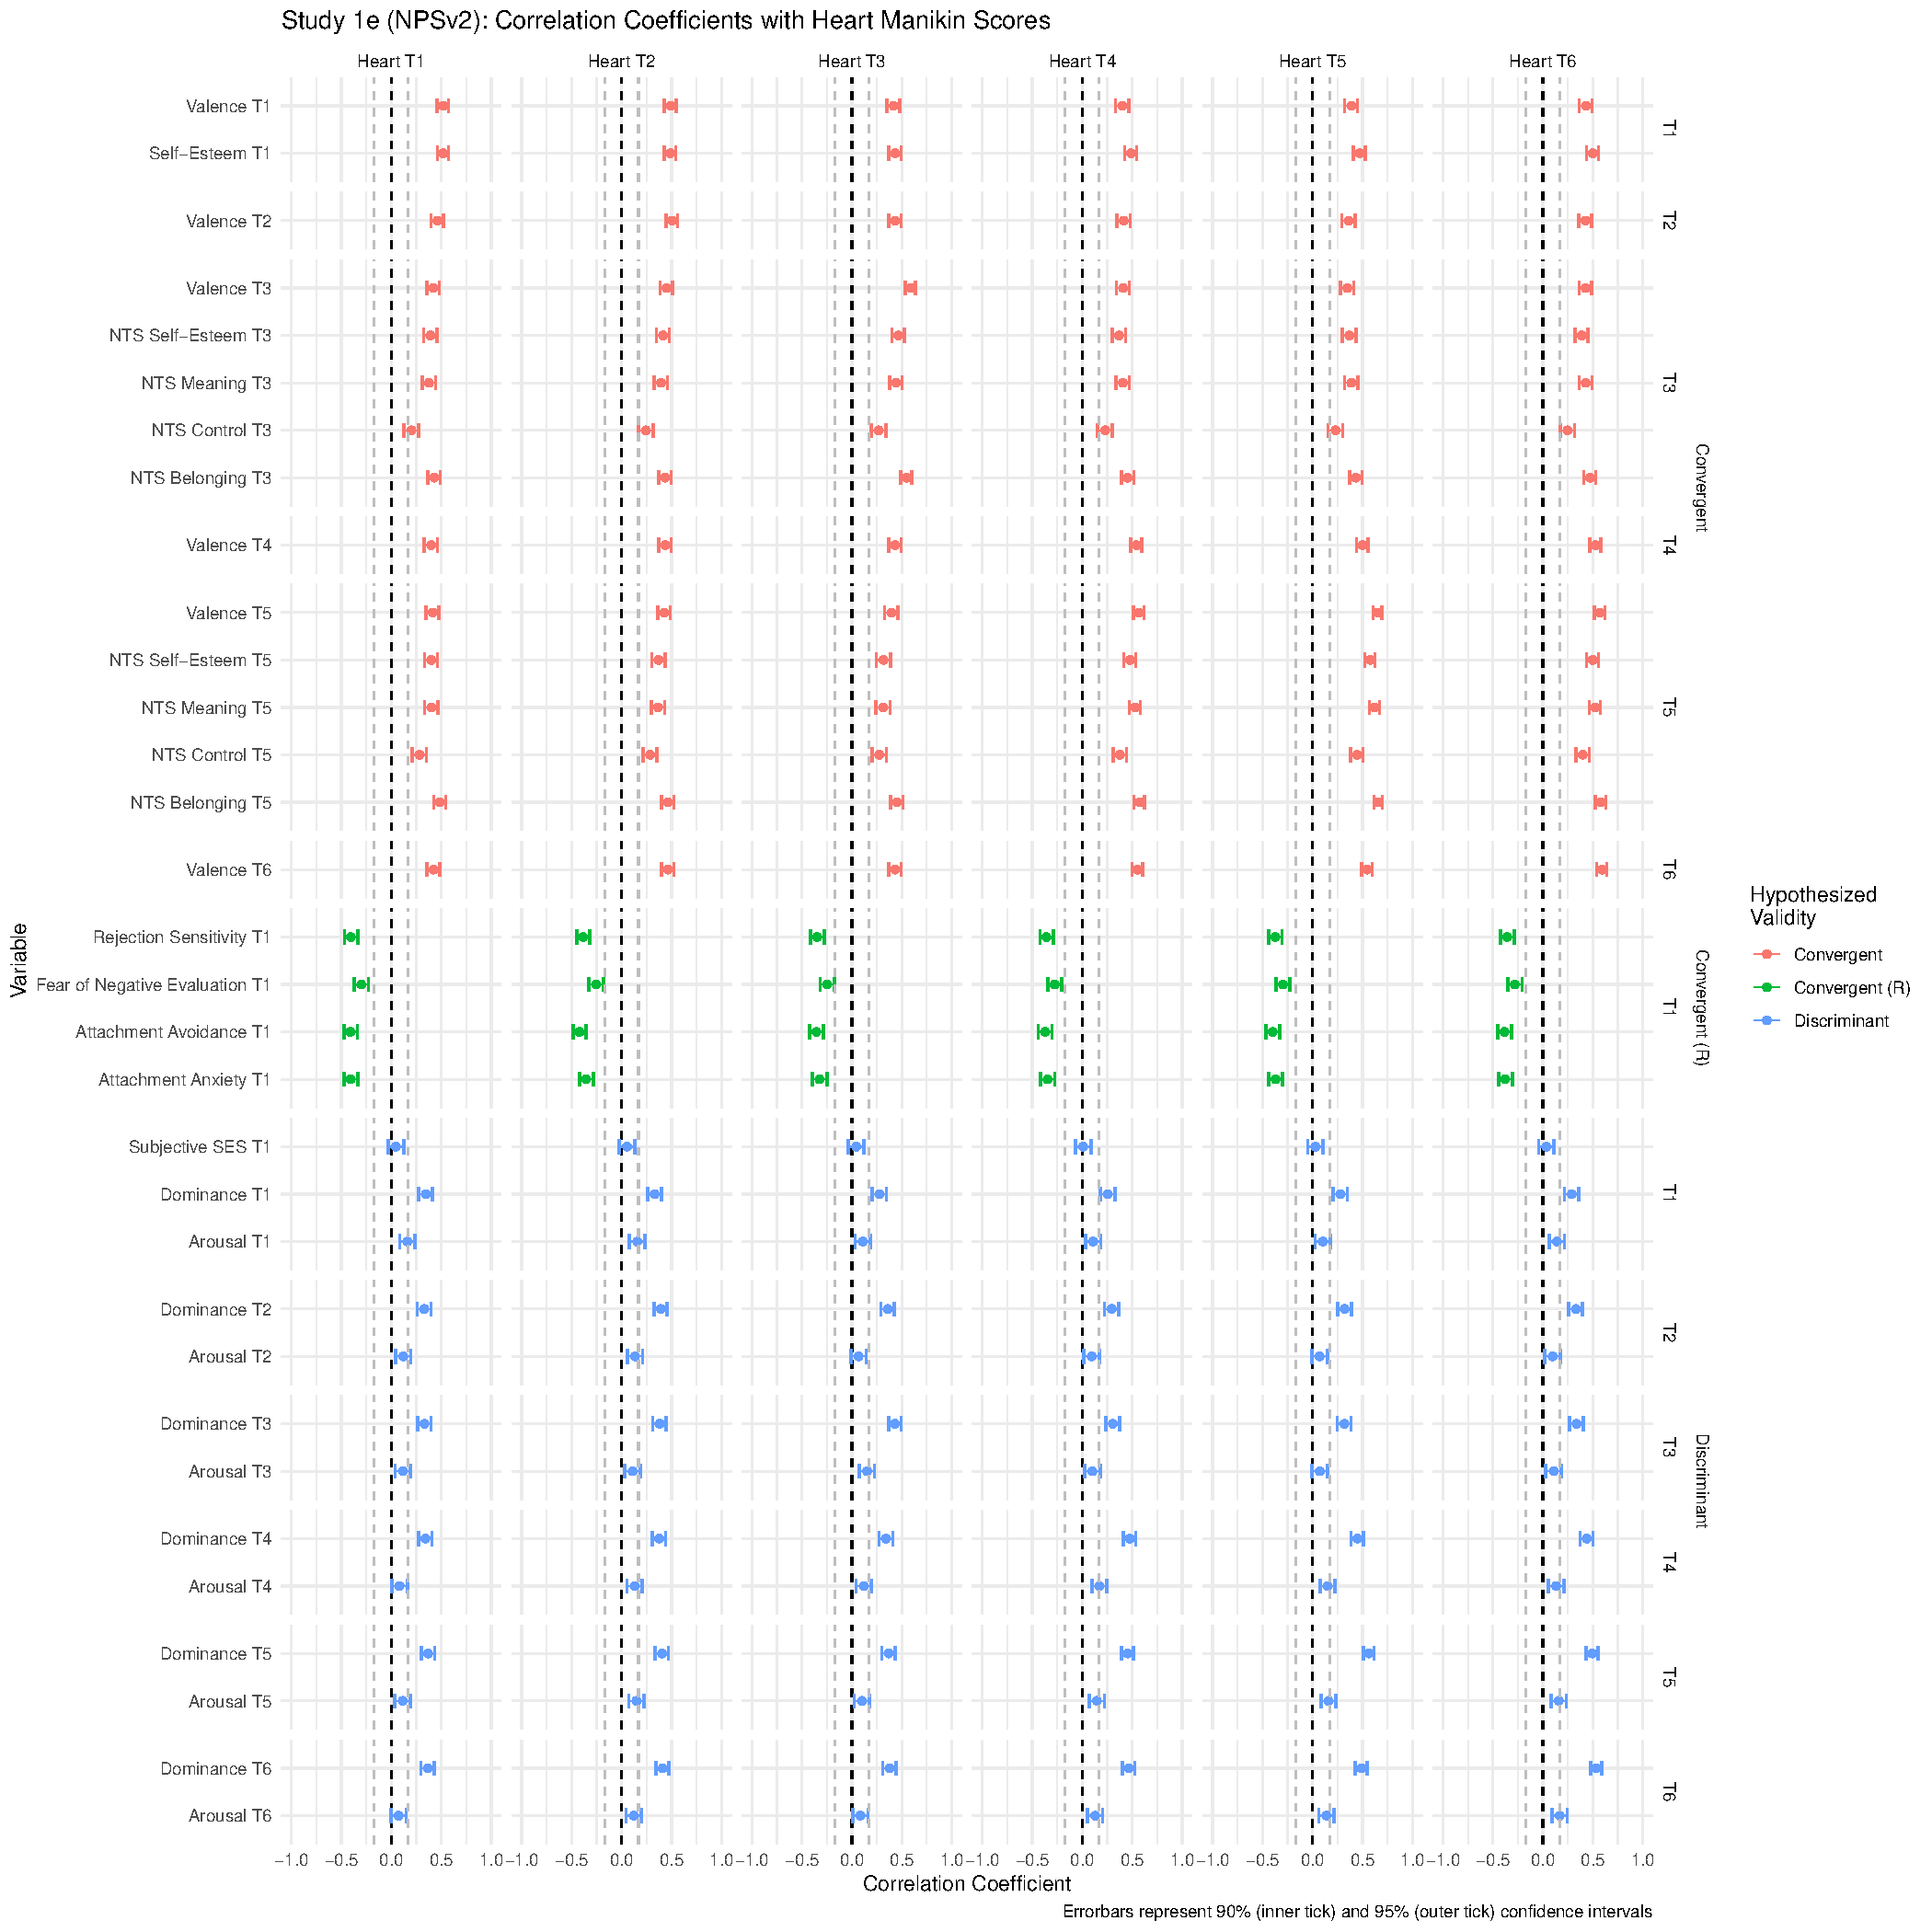
\includegraphics[keepaspectratio]{Sunami-Dissertation_files/figure-latex/appendix-s1e-cor-forestplot-1.pdf}}
\caption{\label{fig:appendix-s1e-cor-forestplot}Study 1e - Forestplot of Correlations between the Measured Variables and the Heart Manikin Scores}
\end{figure}

I explored whether participants reported different levels of belonging across time, depending on the experimental conditions. Figure \ref{fig:appendix-s1e-belonging-plot} shows the Heart Manikin scores across time and the conditions.

\begin{figure}
\centering
\pandocbounded{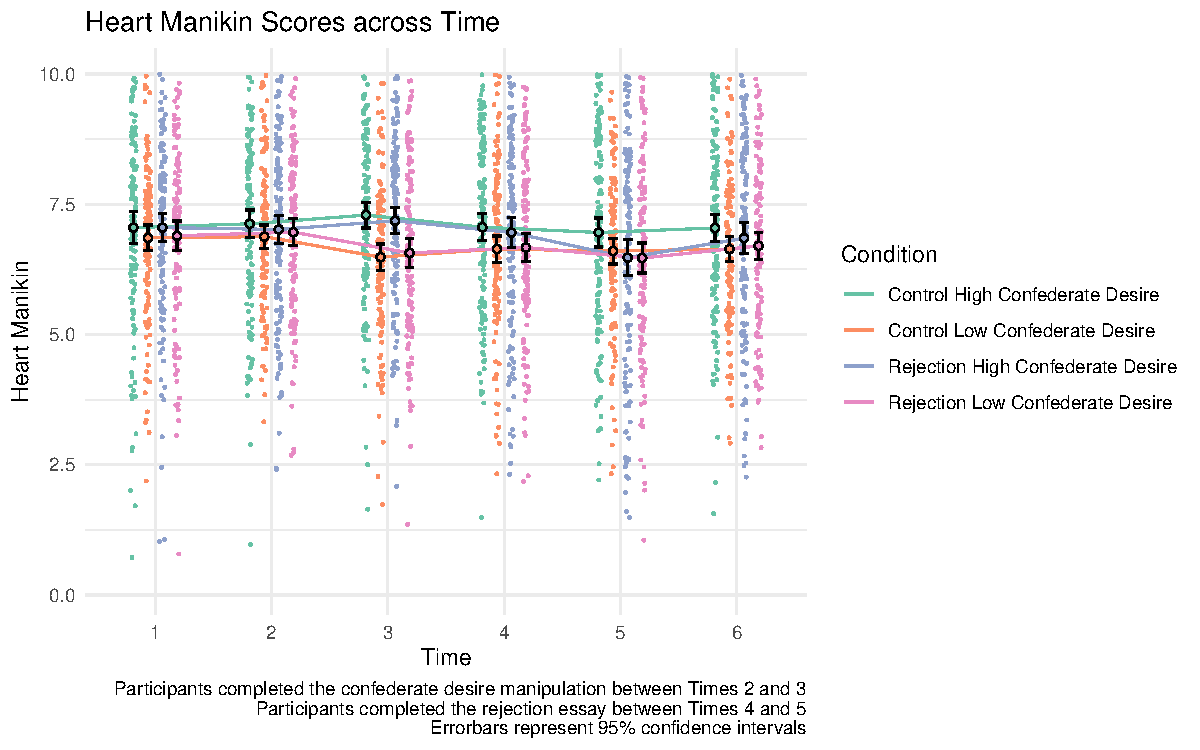
\includegraphics[keepaspectratio]{Sunami-Dissertation_files/figure-latex/appendix-s1e-belonging-plot-1.pdf}}
\caption{\label{fig:appendix-s1e-belonging-plot}Study 1e - Heart Manikin Scores}
\end{figure}

I also explored whether participants reported different levels of need-threat between Time 3 and Time 5. Results are plotted in Figure \ref{fig:s1e-nts-across-time-plot}

\begin{figure}
\centering
\pandocbounded{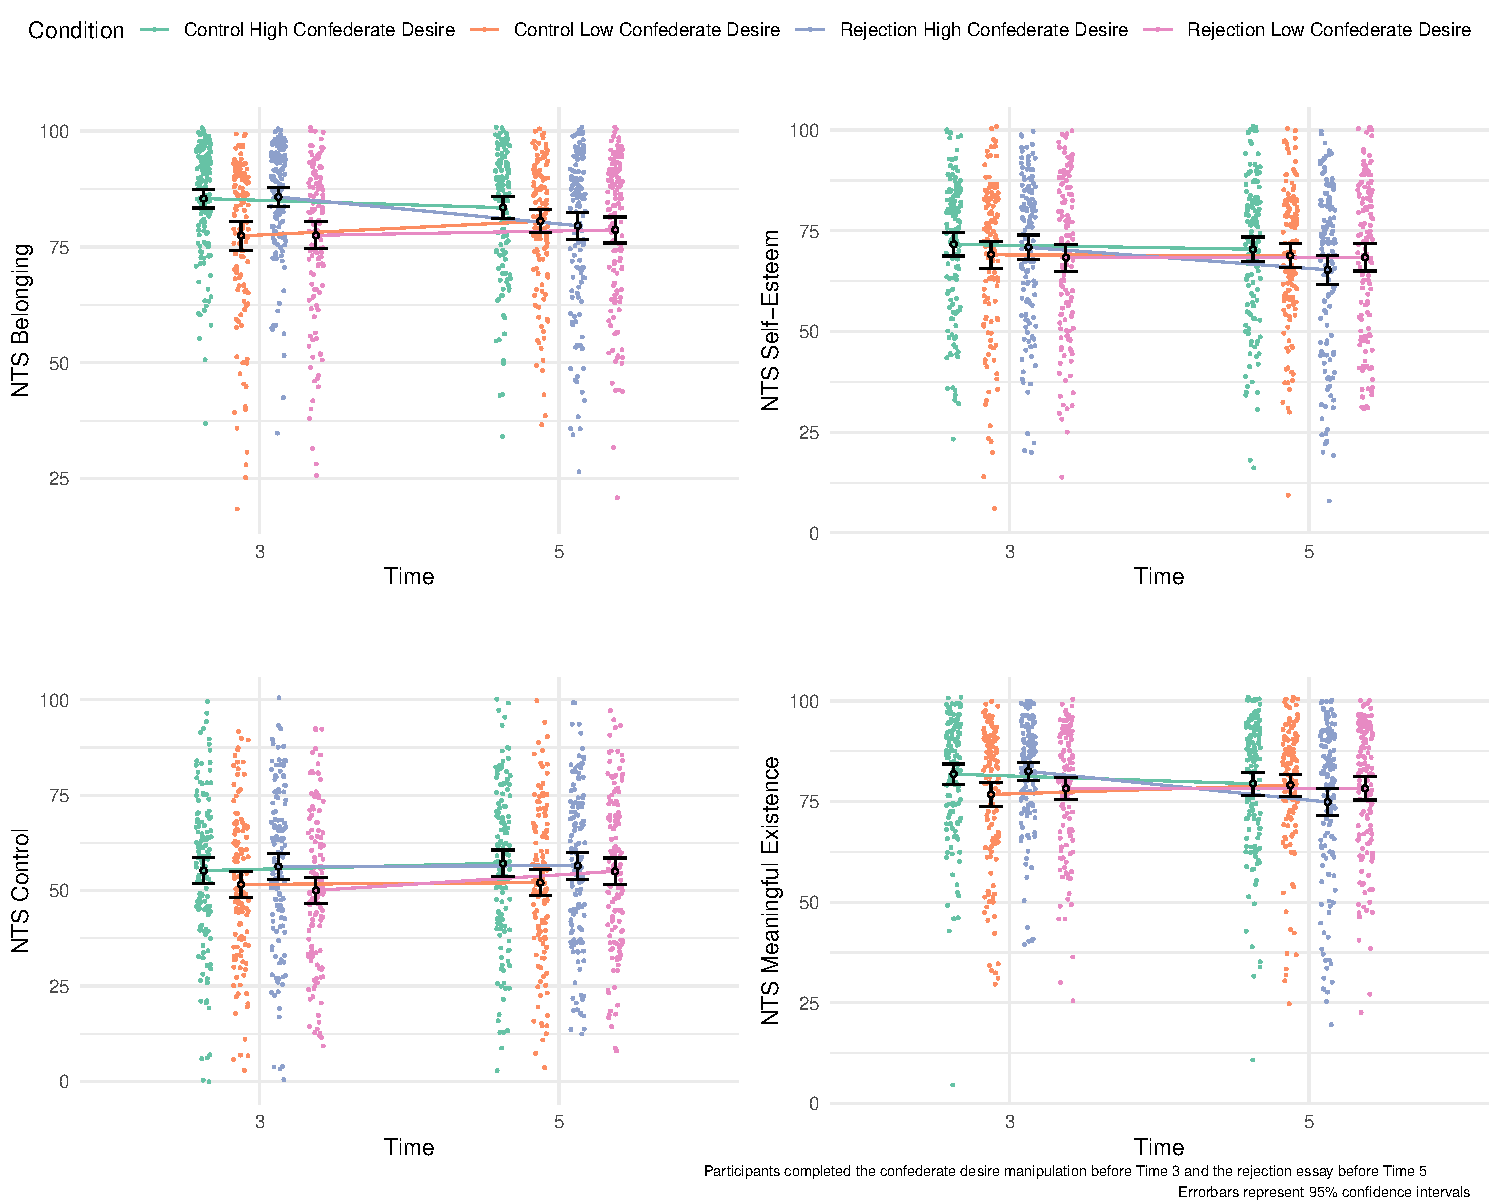
\includegraphics[keepaspectratio]{Sunami-Dissertation_files/figure-latex/s1e-nts-across-time-plot-1.pdf}}
\caption{\label{fig:s1e-nts-across-time-plot}Need-Threat Scores Across Time and Condition}
\end{figure}

I explored whether participants with higher (vs.~lower) self-esteem reported different levels of need-threat at Time 5 (after rejection) in a regression model (predictors: the main effect of rejection, the main effect of self-esteem, and the interaction between rejection and self-esteem). Figure \ref{fig:s1e-nts-t5-mod-by-esteem} shows the results. I did not find evidence of moderation by self-esteem for the effect of social rejection.

\begin{figure}
\centering
\pandocbounded{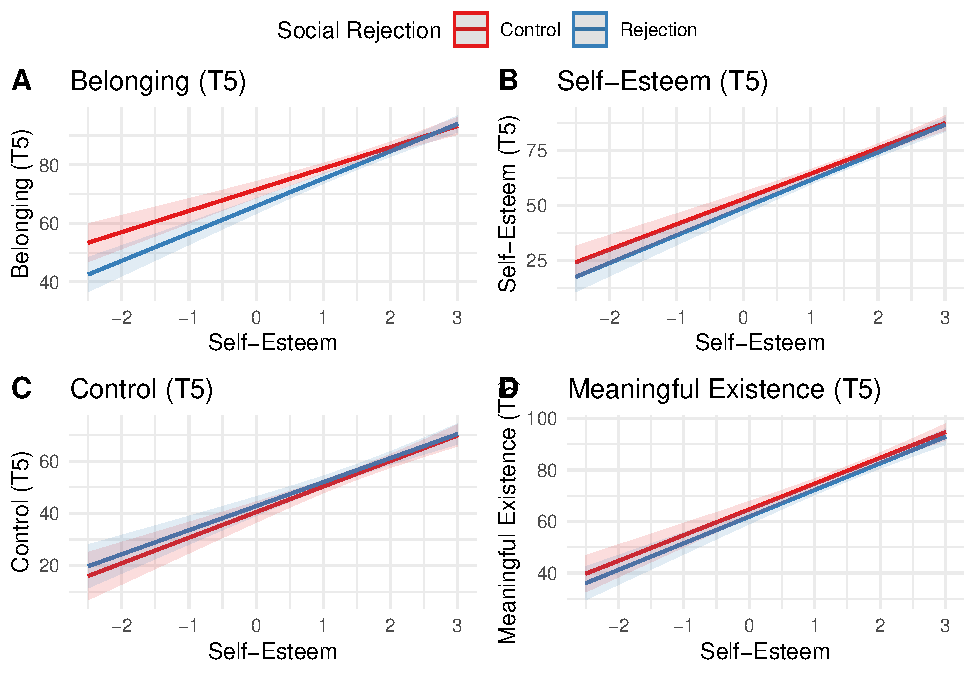
\includegraphics[keepaspectratio]{Sunami-Dissertation_files/figure-latex/s1e-nts-t5-mod-by-esteem-1.pdf}}
\caption{\label{fig:s1e-nts-t5-mod-by-esteem}Study 1e - Self-Esteem as a Possible Moderator for the Effect of Rejection on Need-Threat}
\end{figure}

\section{Study 2}\label{study-2}

\begin{landscape}\begin{table}
\centering
\caption{\label{tab:s2-correlations-table}Bivariate Correlations Among the Measures in Study 2}
\centering
\begin{threeparttable}
\resizebox{\ifdim\width>\linewidth\linewidth\else\width\fi}{!}{
\begin{tabular}[t]{>{\raggedright\arraybackslash}p{1.5in}cccccccccccccccc}
\toprule
\multicolumn{1}{c}{Variable} & \multicolumn{1}{c}{$n$} & \multicolumn{1}{c}{$M$} & \multicolumn{1}{c}{$SD$} & \multicolumn{1}{c}{1} & \multicolumn{1}{c}{2} & \multicolumn{1}{c}{3} & \multicolumn{1}{c}{4} & \multicolumn{1}{c}{5} & \multicolumn{1}{c}{6} & \multicolumn{1}{c}{7} & \multicolumn{1}{c}{8} & \multicolumn{1}{c}{9} & \multicolumn{1}{c}{10} & \multicolumn{1}{c}{11} & \multicolumn{1}{c}{12} & \multicolumn{1}{c}{13}\\
\midrule
1. Heart (T1) & 359 & 6.21 & 1.98 &  &  &  &  &  &  &  &  &  &  &  &  & \\
2. Heart (T2) & 359 & 6.32 & 1.91 & .77* &  &  &  &  &  &  &  &  &  &  &  & \\
3. Valence (T1) & 359 & 5.93 & 1.89 & .72* & .62* &  &  &  &  &  &  &  &  &  &  & \\
4. Valence (T2) & 359 & 6.25 & 1.76 & .57* & .74* & .71* &  &  &  &  &  &  &  &  &  & \\
5. Arousal (T1) & 359 & 4.22 & 1.69 & .06 & .06 & .16* & .09 &  &  &  &  &  &  &  &  & \\
\addlinespace
6. Arousal (T2) & 359 & 4.92 & 1.89 & .00 & .13* & .08 & .19* & .58* &  &  &  &  &  &  &  & \\
7. Dominance (T1) & 359 & 5.83 & 1.65 & .30* & .31* & .31* & .30* & .14* & .19* &  &  &  &  &  &  & \\
8. Dominance (T2) & 359 & 6.10 & 1.63 & .27* & .38* & .27* & .39* & .08 & .25* & .85* &  &  &  &  &  & \\
9. IOS & 211 & 3.07 & 1.76 & -.13 & -.04 & -.04 & .07 & -.03 & .13 & .13 & .12 &  &  &  &  & \\
10. PSI & 210 & 2.21 & 0.71 & -.11 & -.04 & -.03 & .12 & -.10 & .17* & -.01 & .01 & .60* &  &  &  & \\
\addlinespace
11. Narrative Eng. & 357 & 0.63 & 0.87 & .00 & -.01 & .06 & .08 & .04 & .13* & -.01 & .03 & .27* & .37* &  &  & \\
12. Immersion & 359 & 1.92 & 1.24 & .08 & .14* & .12* & .22* & -.05 & .10 & .08 & .14* & .24* & .29* & .40* &  & \\
13. Social World & 358 & -0.12 & 1.82 & .02 & .05 & .05 & .15* & -.04 & .13* & -.02 & .04 & .48* & .57* & .41* & .28* & \\
14. Enjoyment & 359 & 2.31 & 0.72 & .11* & .15* & .16* & .29* & -.02 & .06 & .13* & .15* & .21* & .27* & .37* & .41* & .31*\\
\bottomrule
\end{tabular}}
\begin{tablenotes}[para]
\item \textit{Note.} 
\item The Ns for IOS and PSI are smaller since only people who indicated they interacted with a non-player character saw these questions. IOS = Inclusion of the Other in Self Scale. PSI = Parasocial Interactrion-Process Scale. Narrative Eng. = Narrative Engagement.
\end{tablenotes}
\end{threeparttable}
\end{table}
\end{landscape}

\subsection{Bivariate Scatter Plot Matrix}\label{bivariate-scatter-plot-matrix}

\begin{figure}
\centering
\pandocbounded{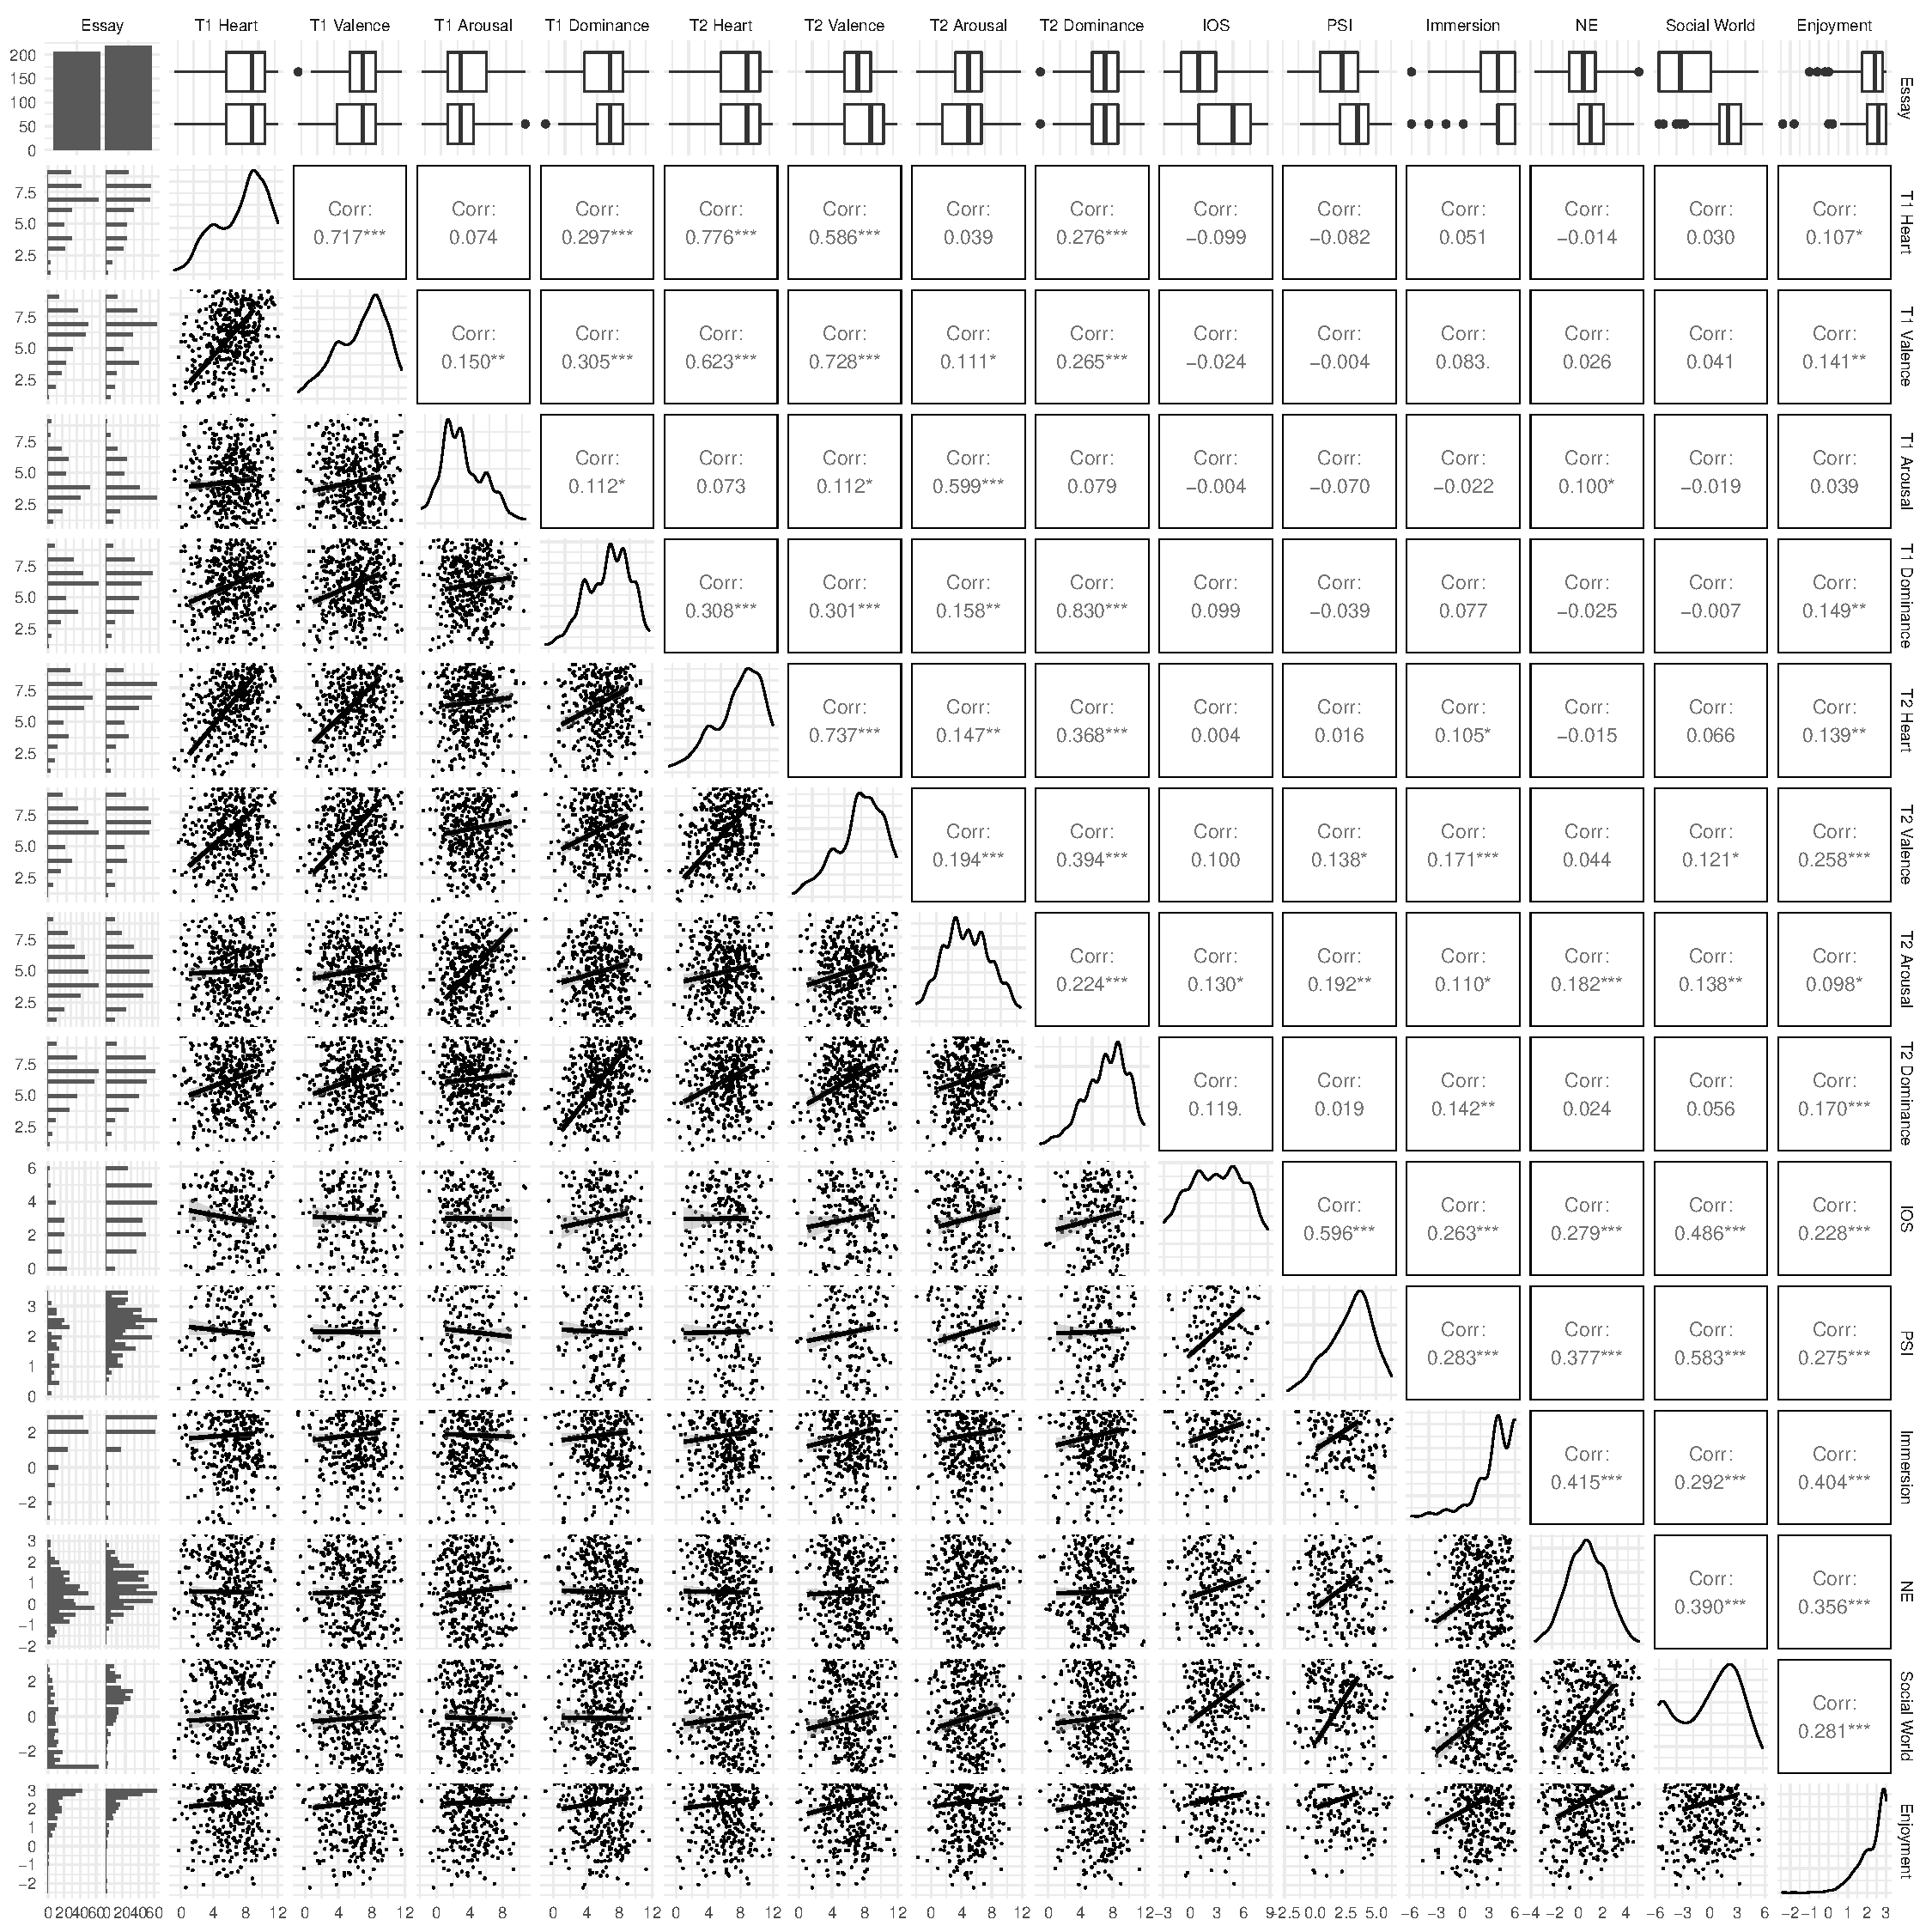
\includegraphics[keepaspectratio]{Sunami-Dissertation_files/figure-latex/s2-matplot-1.pdf}}
\caption{\label{fig:s2-matplot}Matrix Plot for Study 2 Variables}
\end{figure}

\begin{figure}
\centering
\pandocbounded{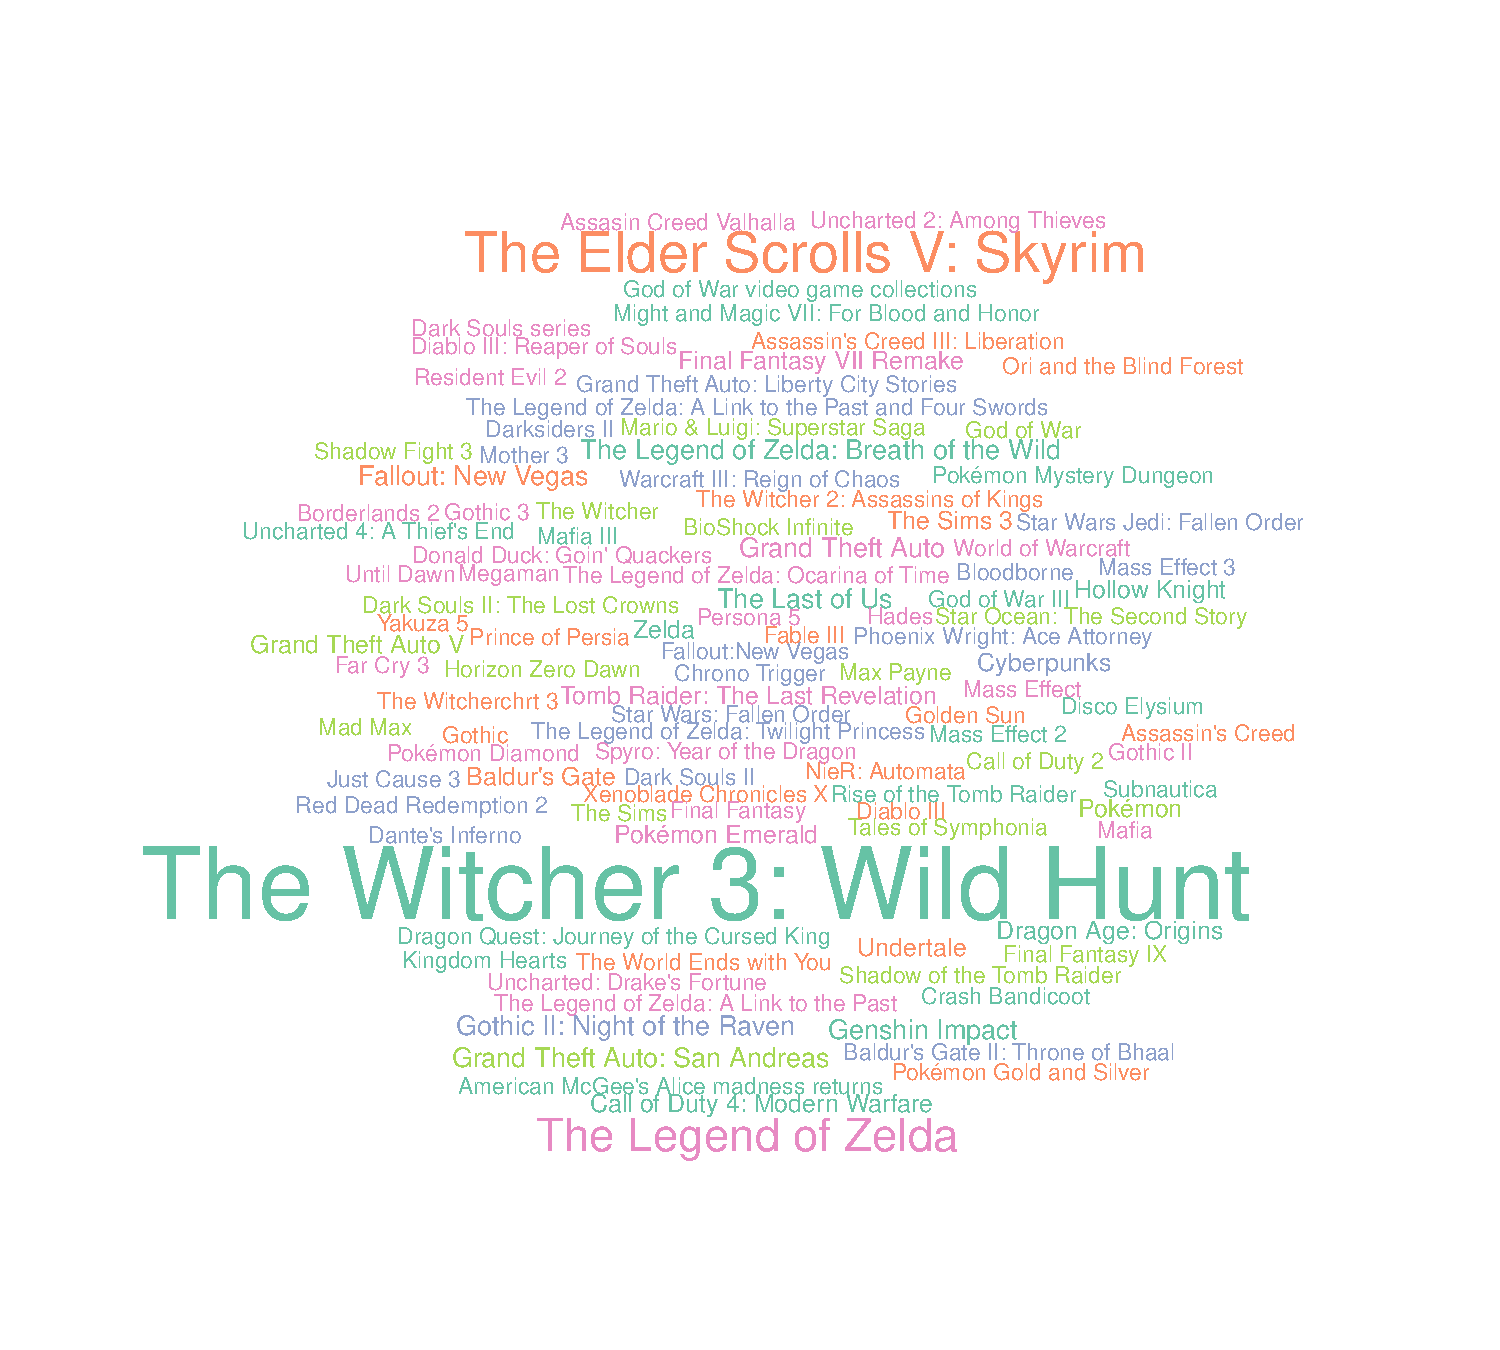
\includegraphics[keepaspectratio]{Sunami-Dissertation_files/figure-latex/s2-word-cloud-1.pdf}}
\caption{\label{fig:s2-word-cloud}Word Cloud for Game Titles for the Social Surrogate Condition}
\end{figure}

\begin{figure}
\centering
\pandocbounded{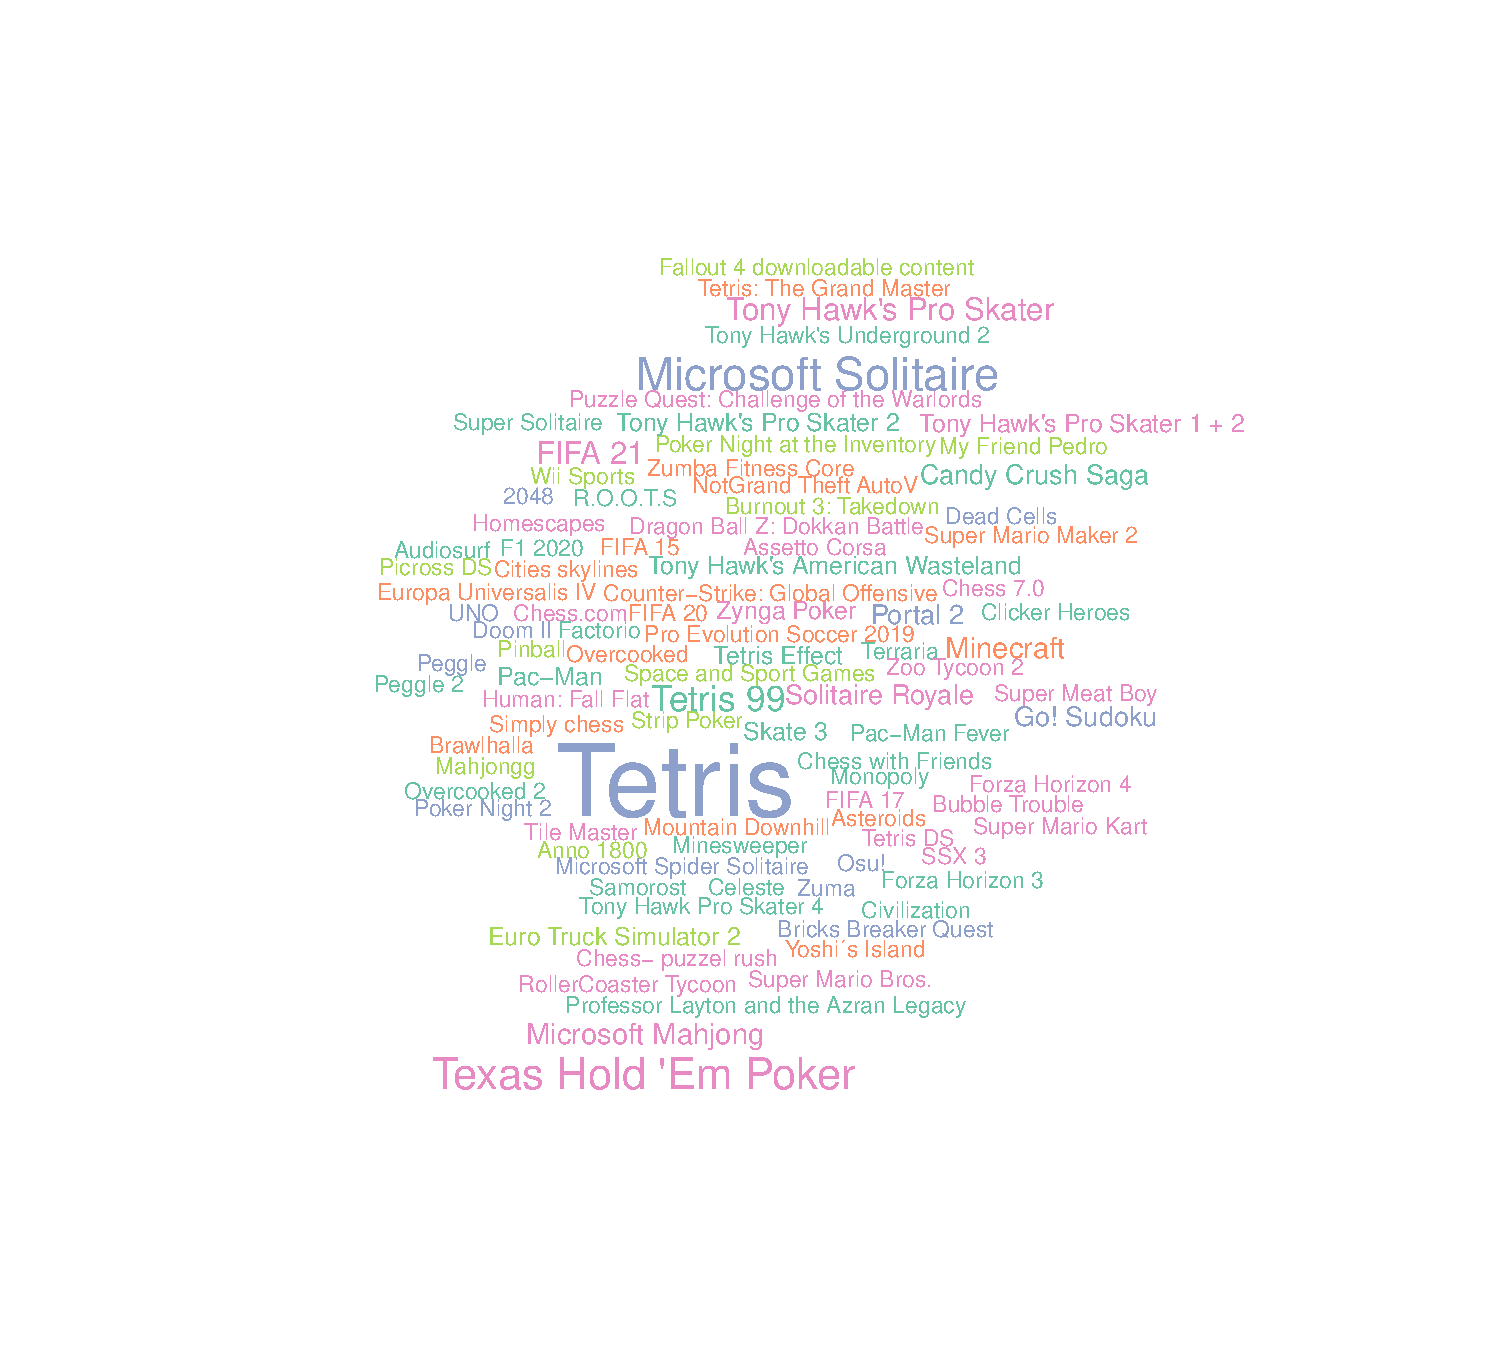
\includegraphics[keepaspectratio]{Sunami-Dissertation_files/figure-latex/s2-word-cloud-nonsurrogate-1.pdf}}
\caption{\label{fig:s2-word-cloud-nonsurrogate}Word Cloud for Game Titles for the Non-Social Surrogate Condition}
\end{figure}

\subsection{Main Analysis with Excluded Participants}\label{main-analysis-with-excluded-participants}

In the main analysis, I excluded participants based on the preregistered exclusion procedure. Here, I report results including all participants. I used the entire dataset including excluded participats to perform Welch's \emph{t}-test to compare the post-esaay Heart Manikin scores (Time 2) between the participants who wrote about the social surrogacy video game and those who wrote about the non-social surrogacy video game. Results were consistent with the analysis without the exculuded participants: participants who wrote about the social surrogacy game () reported similar levels of belonging compared with those who wrote about a non-surrogacy game (, \emph{t}(417.2) = -0.35, \emph{p} = .724).

\subsection{Natural Language Processsing for Essays}\label{natural-language-processsing-for-essays}

I used natural language processing to explore words used in the video game essays. Figure \ref{fig:s2-nlp-plot} shows the proportion of the words used within each essay conditions.
Words such as ``character'' and ``story'' appeared more frequently in the social surrogate essays compared to non-social surrogate essays. On the other hand, words such as ``cards'', ``goal'' appeared more frequently in the non-social surrogate essays than in social surrogate essays.

\begin{figure}
\centering
\pandocbounded{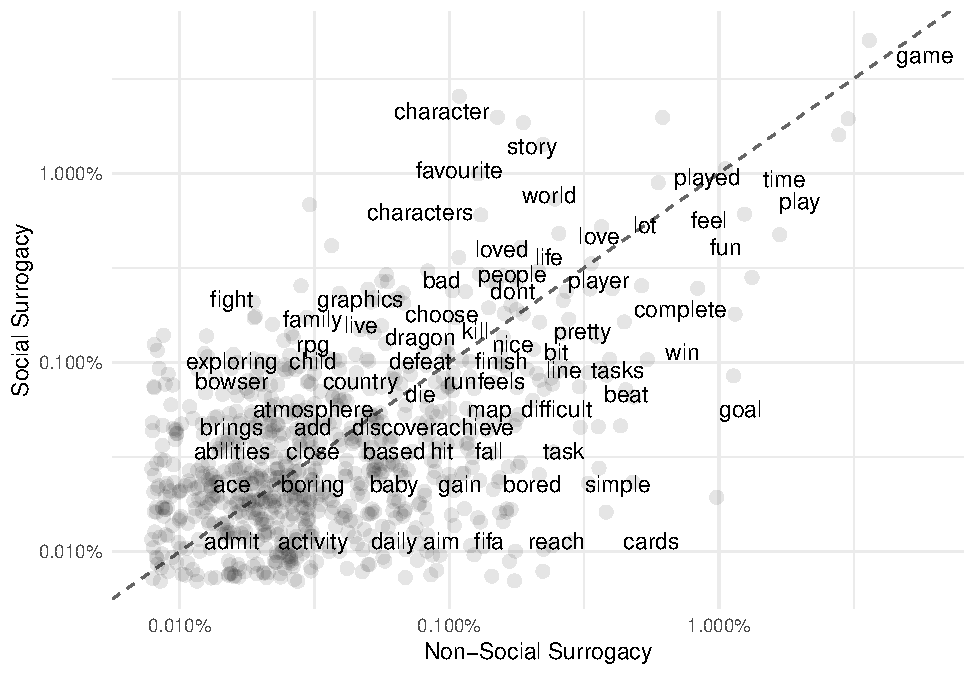
\includegraphics[keepaspectratio]{Sunami-Dissertation_files/figure-latex/s2-nlp-plot-1.pdf}}
\caption{\label{fig:s2-nlp-plot}Proportions of Words Used in Participants Essays Within Each Video Game Conditions. Words along the dashed line appeared equally in across social surrogacy and non-social surrogacy conditions. Words in the upper diagonal appeared more frequently in the social surrogacy condition than in the non-social surrogacy condition. Words in the lower diagnoal appeared more frequently in the non-social surrogacy condition.}
\end{figure}

\subsection{Exit Questions}\label{exit-questions}

Participants saw two debrief questions, one referring to the purpose of the study, and another asking them to share anything about the study. I presented the debriefing questions in a randomized order to explore whether participants provided different amount of information if they were asked about the purpose of the study first, or they were asked to share anything. Results are presented in Figure \ref{fig:s2-exit-questions-plot}. In writing about the purpose of the study, participants who were asked about the purpose of the study first left a longer answer than those who were asked to share anything first.

\begin{figure}
\centering
\pandocbounded{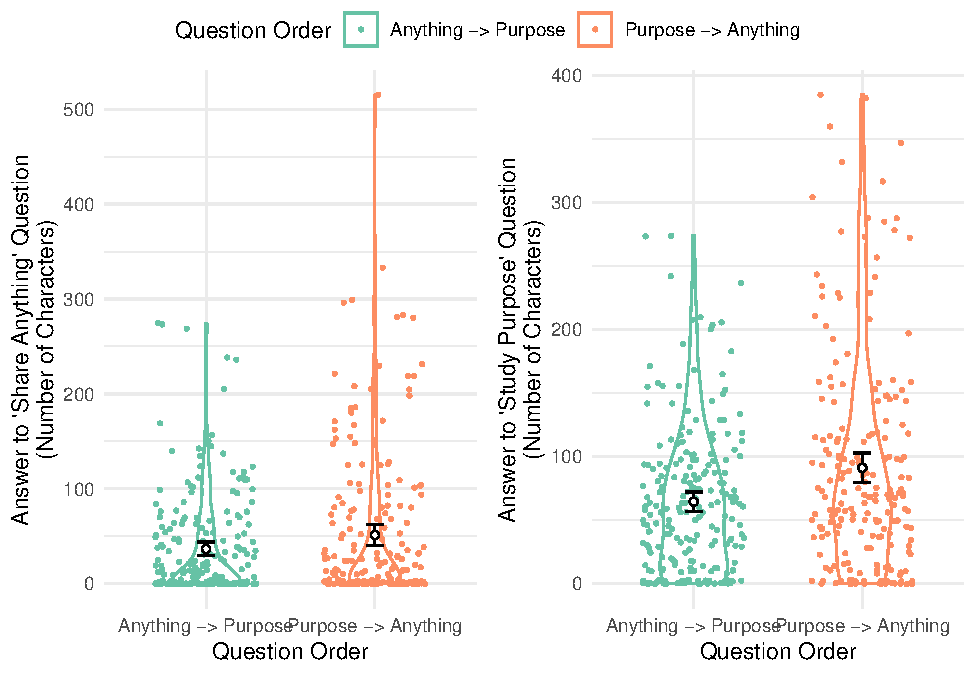
\includegraphics[keepaspectratio]{Sunami-Dissertation_files/figure-latex/s2-exit-questions-plot-1.pdf}}
\caption{\label{fig:s2-exit-questions-plot}Study 2 - Lengths of Participant Answers to Exit Questions Across Question Order}
\end{figure}

\section{Study 3}\label{study-3}

\begin{landscape}\begin{table}
\centering
\caption{\label{tab:appendix-s3-correlations-table}Bivariate Correlations among the Measures in Study 3}
\centering
\begin{threeparttable}
\resizebox{\ifdim\width>\linewidth\linewidth\else\width\fi}{!}{
\begin{tabular}[t]{>{\raggedright\arraybackslash}p{1.2in}ccccccccccccccc}
\toprule
\multicolumn{1}{c}{Variable} & \multicolumn{1}{c}{$n$} & \multicolumn{1}{c}{$M$} & \multicolumn{1}{c}{$SD$} & \multicolumn{1}{c}{1} & \multicolumn{1}{c}{2} & \multicolumn{1}{c}{3} & \multicolumn{1}{c}{4} & \multicolumn{1}{c}{5} & \multicolumn{1}{c}{6} & \multicolumn{1}{c}{7} & \multicolumn{1}{c}{8} & \multicolumn{1}{c}{9} & \multicolumn{1}{c}{10} & \multicolumn{1}{c}{11} & \multicolumn{1}{c}{12}\\
\midrule
1. Heart (T1) & 344 & 6.45 & 1.90 &  &  &  &  &  &  &  &  &  &  &  & \\
2. Heart (T2) & 344 & 6.24 & 1.87 & .66* &  &  &  &  &  &  &  &  &  &  & \\
3. Valence (T1) & 344 & 6.00 & 1.91 & .65* & .46* &  &  &  &  &  &  &  &  &  & \\
4. Valence (T2) & 344 & 5.64 & 2.30 & .28* & .57* & .33* &  &  &  &  &  &  &  &  & \\
5. Arousal (T1) & 344 & 4.24 & 1.76 & .28* & .21* & .32* & .22* &  &  &  &  &  &  &  & \\
\addlinespace
6. Arousal (T2) & 344 & 5.01 & 1.97 & .17* & .33* & .17* & .52* & .43* &  &  &  &  &  &  & \\
7. Dominance (T1) & 343 & 6.04 & 1.63 & .33* & .28* & .33* & .16* & .15* & .07 &  &  &  &  &  & \\
8. Dominance (T2) & 343 & 6.25 & 1.72 & .19* & .51* & .18* & .49* & .11* & .29* & .51* &  &  &  &  & \\
9. IOS & 272 & 2.81 & 1.72 & .08 & .15* & .06 & .27* & .14* & .26* & .08 & .29* &  &  &  & \\
10. Immersion & 344 & 0.21 & 1.81 & .10 & .33* & .11* & .53* & .10 & .33* & -.04 & .27* & .32* &  &  & \\
\addlinespace
11. Social World & 337 & -0.23 & 1.52 & .13* & .33* & .10 & .53* & .11* & .35* & -.02 & .31* & .32* & .77* &  & \\
12. Identification & 315 & -0.90 & 0.96 & .07 & .24* & .07 & .39* & .18* & .30* & .05 & .27* & .34* & .50* & .60* & \\
13. Enjoyment & 342 & -0.43 & 1.62 & .03 & .28* & .04 & .55* & -.01 & .31* & -.08 & .29* & .25* & .71* & .79* & .63*\\
\bottomrule
\end{tabular}}
\begin{tablenotes}[para]
\item \textit{Note.} 
\item *p .05. IOS = Inclusion of the Other in Self Scale. The N of IOS is smaller since only those interacted with an NPC answered this question. The Ns for dominance, social world, identification, and enjoyment are smaller due to programming errors and participants skipping questions.
\end{tablenotes}
\end{threeparttable}
\end{table}
\end{landscape}

\begin{figure}
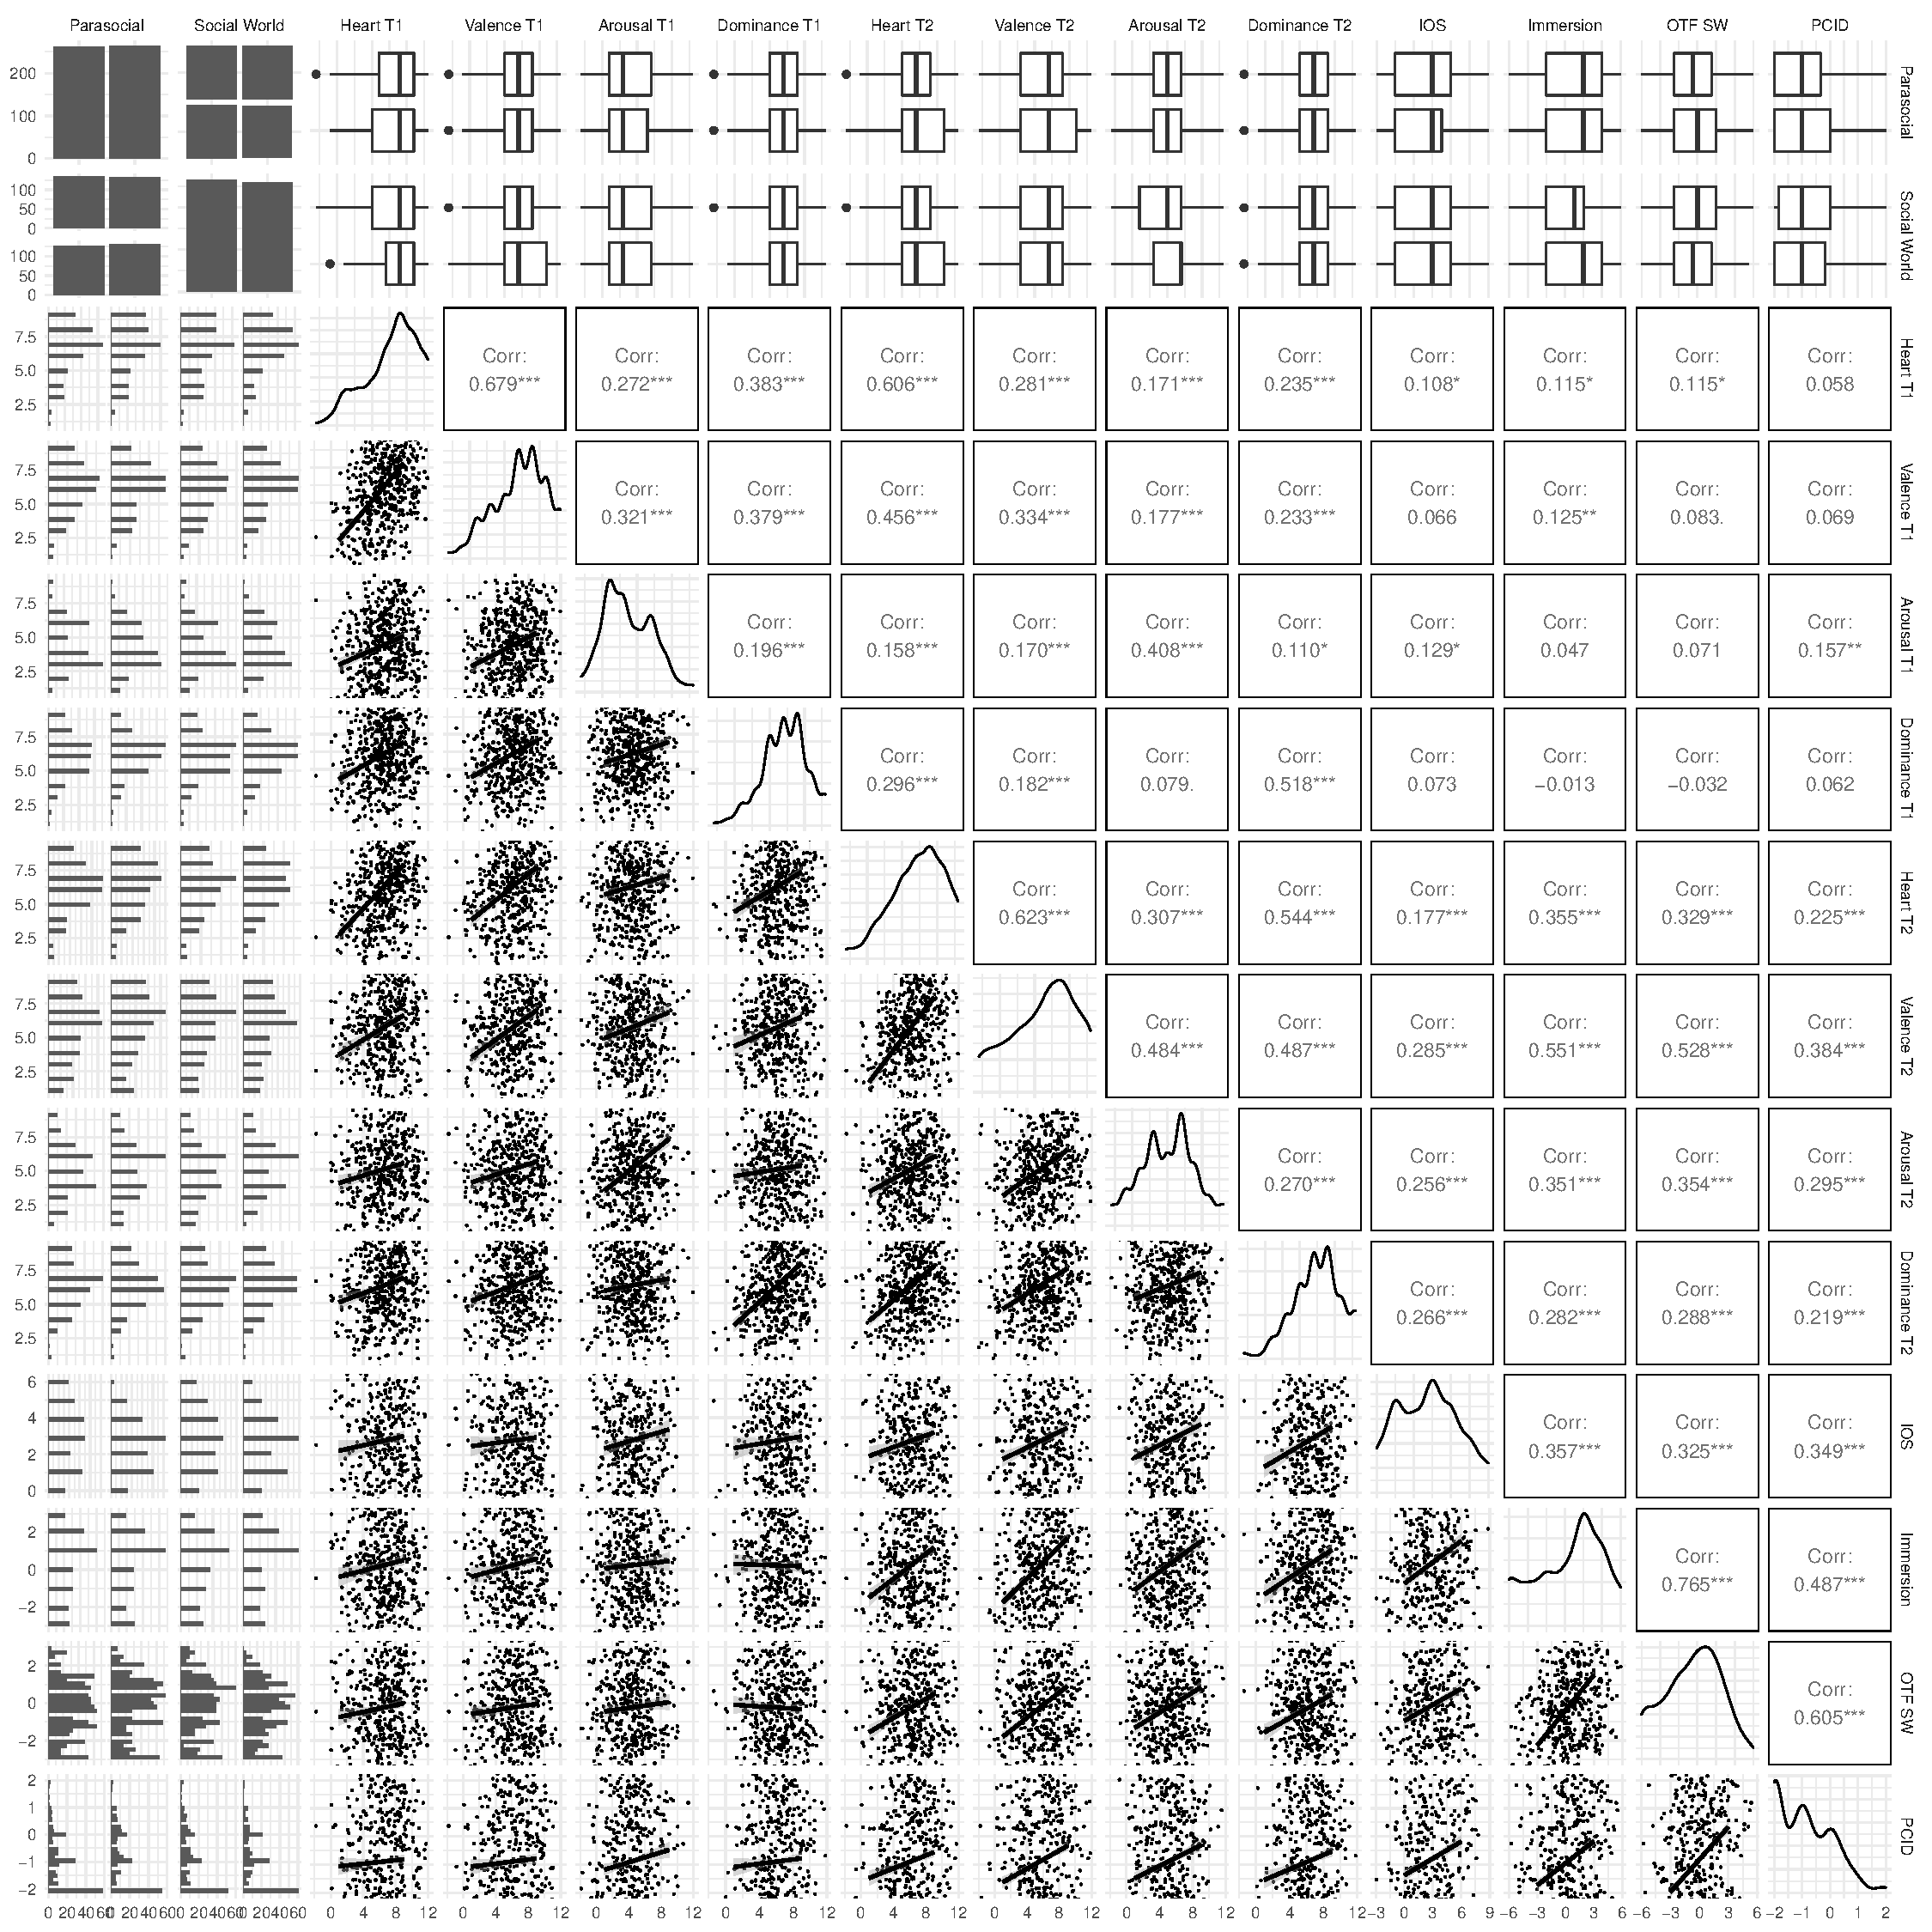
\includegraphics[width=1\linewidth]{Sunami-Dissertation_files/figure-latex/appendix-s3-ggpairs-1} \caption{Study 3 - Bivariate Scatter Plot Matrix}\label{fig:appendix-s3-ggpairs}
\end{figure}

\chapter{Software Programs Used}\label{software-programs-used}

In writing my dissertation, I used R packages and software programs developed by the following authors: Plate \& Heiberger (\citeproc{ref-R-abind}{2024}), Chetverikov (\citeproc{ref-R-apastats}{2024}), R Core Team (\citeproc{ref-R-base}{2024}), Xie (\citeproc{ref-R-bookdown}{2024}), Robinson et al. (\citeproc{ref-R-broom}{2024}), Bolker \& Robinson (\citeproc{ref-R-broom.mixed}{2024}), Fox et al. (\citeproc{ref-R-car}{2024}), Fox et al. (\citeproc{ref-R-carData}{2022}), M. Lang (\citeproc{ref-R-checkmate}{2024}), Arslan (\citeproc{ref-R-codebook}{2024}), Kuhn et al. (\citeproc{ref-R-corrr}{2022}), Barrett et al. (\citeproc{ref-R-data.table}{2024}), Wickham, François, et al. (\citeproc{ref-R-dplyr}{2023}), Ben-Shachar et al. (\citeproc{ref-R-effectsize}{2024}), Lenth (\citeproc{ref-R-emmeans}{2024}), Fox et al. (\citeproc{ref-R-english}{2021}), Wickham (\citeproc{ref-R-forcats}{2023a}), Gordon \& Lumley (\citeproc{ref-R-forestplot}{2024}), Schloerke et al. (\citeproc{ref-R-GGally}{2024}), Jeppson et al. (\citeproc{ref-R-ggmosaic}{2021}), Wickham, Chang, et al. (\citeproc{ref-R-ggplot2}{2024}), Kassambara (\citeproc{ref-R-ggpubr}{2023}), Wilke \& Wiernik (\citeproc{ref-R-ggtext}{2022}), Müller (\citeproc{ref-R-here}{2020}), Harrell (\citeproc{ref-R-Hmisc}{2024}), Zhu (\citeproc{ref-R-kableExtra}{2024}), Bates, Maechler, Bolker, et al. (\citeproc{ref-R-lme4}{2024}), Kuznetsova et al. (\citeproc{ref-R-lmerTest}{2020}), Spinu et al. (\citeproc{ref-R-lubridate}{2024}), Bates, Maechler, \& Jagan (\citeproc{ref-R-Matrix}{2024}), Aden-Buie (\citeproc{ref-R-metathis}{2023}), Wickham \& Henry (\citeproc{ref-R-purrr}{2023}), Neuwirth (\citeproc{ref-R-RColorBrewer}{2022}), Wickham, Hester, et al. (\citeproc{ref-R-readr}{2024}), Allaire et al. (\citeproc{ref-R-rmarkdown}{2024}), Wickham, Pedersen, et al. (\citeproc{ref-R-scales}{2023}), Wickham (\citeproc{ref-R-stringr}{2023b}), Müller \& Wickham (\citeproc{ref-R-tibble}{2023}), Wickham, Vaughan, et al. (\citeproc{ref-R-tidyr}{2024}), Robinson \& Silge (\citeproc{ref-R-tidytext}{2024}), Wickham (\citeproc{ref-R-tidyverse}{2023c}), Fellows (\citeproc{ref-R-wordcloud}{2018}), Xie (\citeproc{ref-bookdown2016}{2016}), Fox \& Weisberg (\citeproc{ref-car2019}{2019}), M. Lang (\citeproc{ref-checkmate}{2017}), Ruben C. Arslan (\citeproc{ref-codebook2019}{2019}), Ben-Shachar et al. (\citeproc{ref-effectsize2020}{2020}), Wickham (\citeproc{ref-ggplot22016}{2016}), Bates et al. (\citeproc{ref-lme42015}{2015}), Kuznetsova et al. (\citeproc{ref-lmerTest2017}{2017}), Grolemund \& Wickham (\citeproc{ref-lubridate2011}{2011}), Xie et al. (\citeproc{ref-rmarkdown2018}{2018}), Xie et al. (\citeproc{ref-rmarkdown2020}{2020}), Silge \& Robinson (\citeproc{ref-tidytext2016}{2016}), Wickham et al. (\citeproc{ref-tidyverse2019}{2019})

\chapter{Instituional Review Board Approval Letters}\label{instituional-review-board-approval-letters}

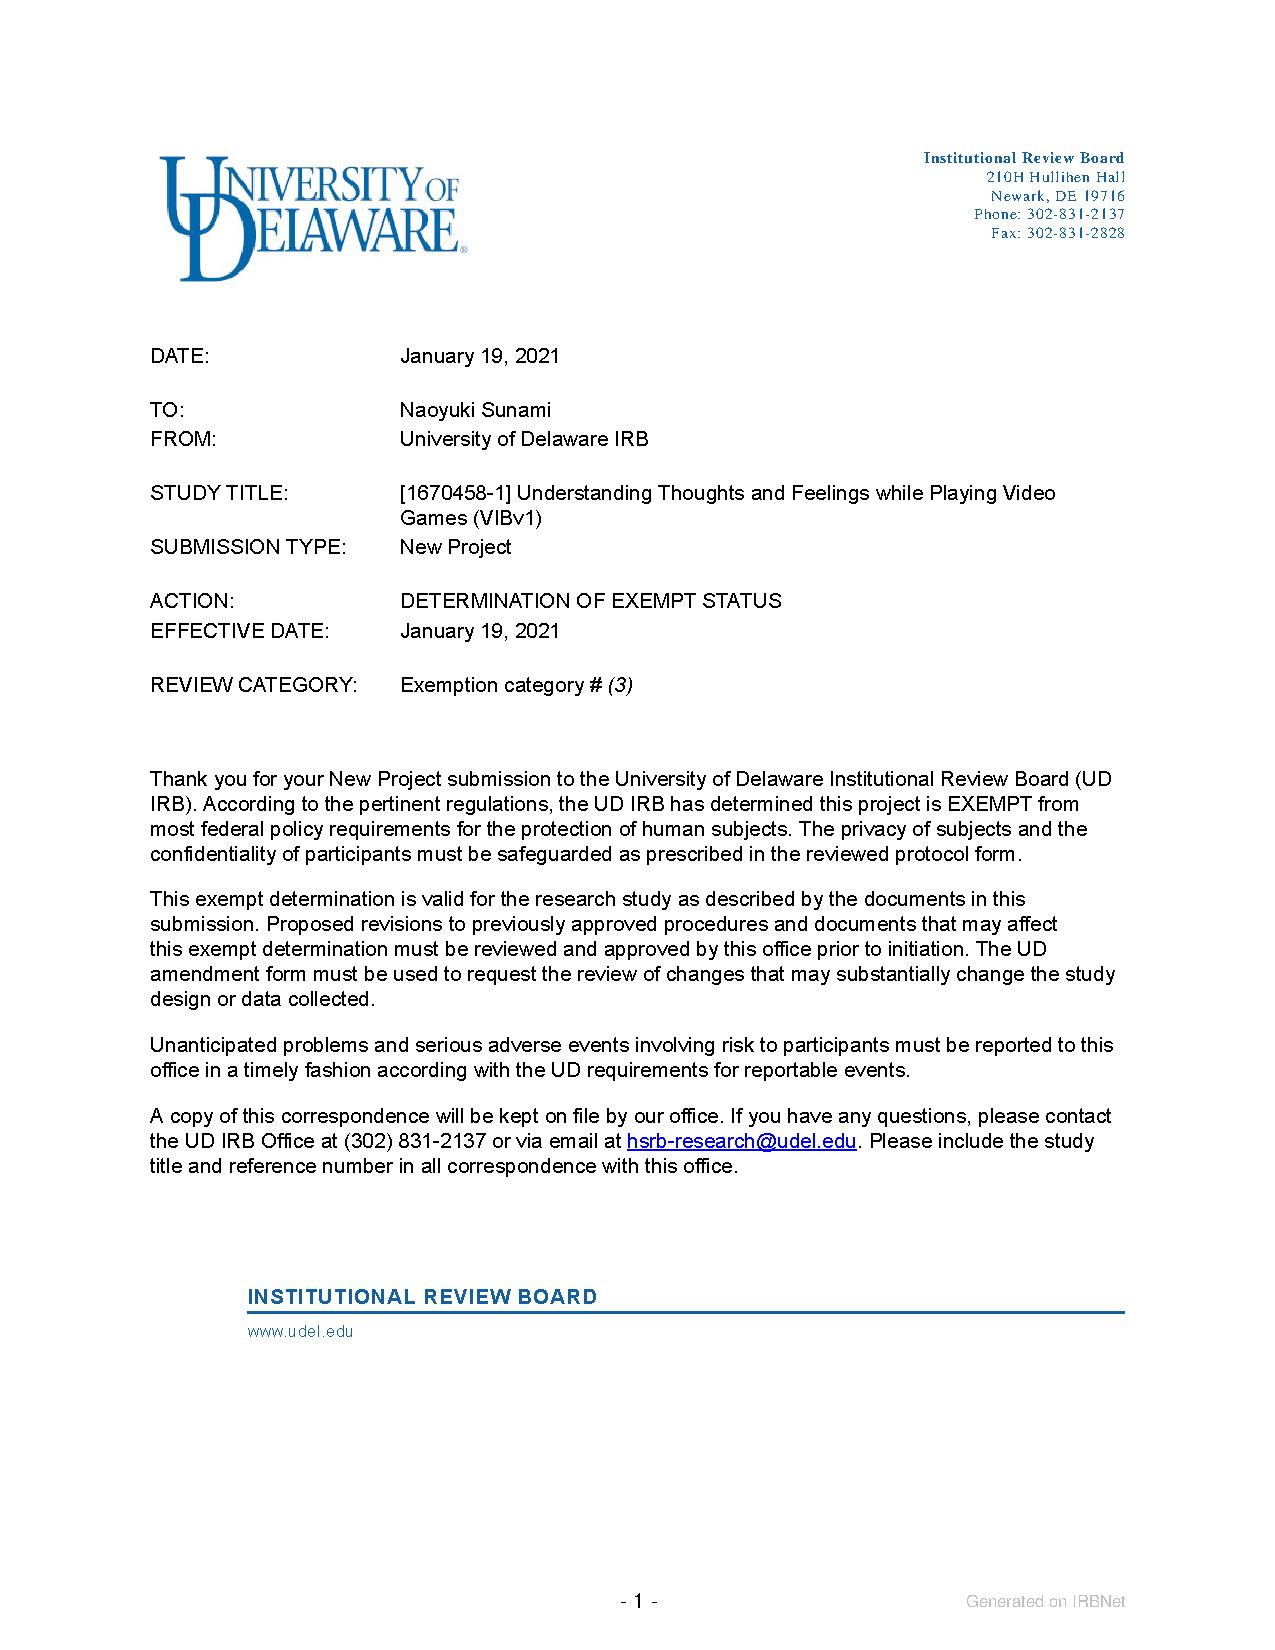
\includegraphics[width=1\linewidth]{pdf/IRB_letter1}

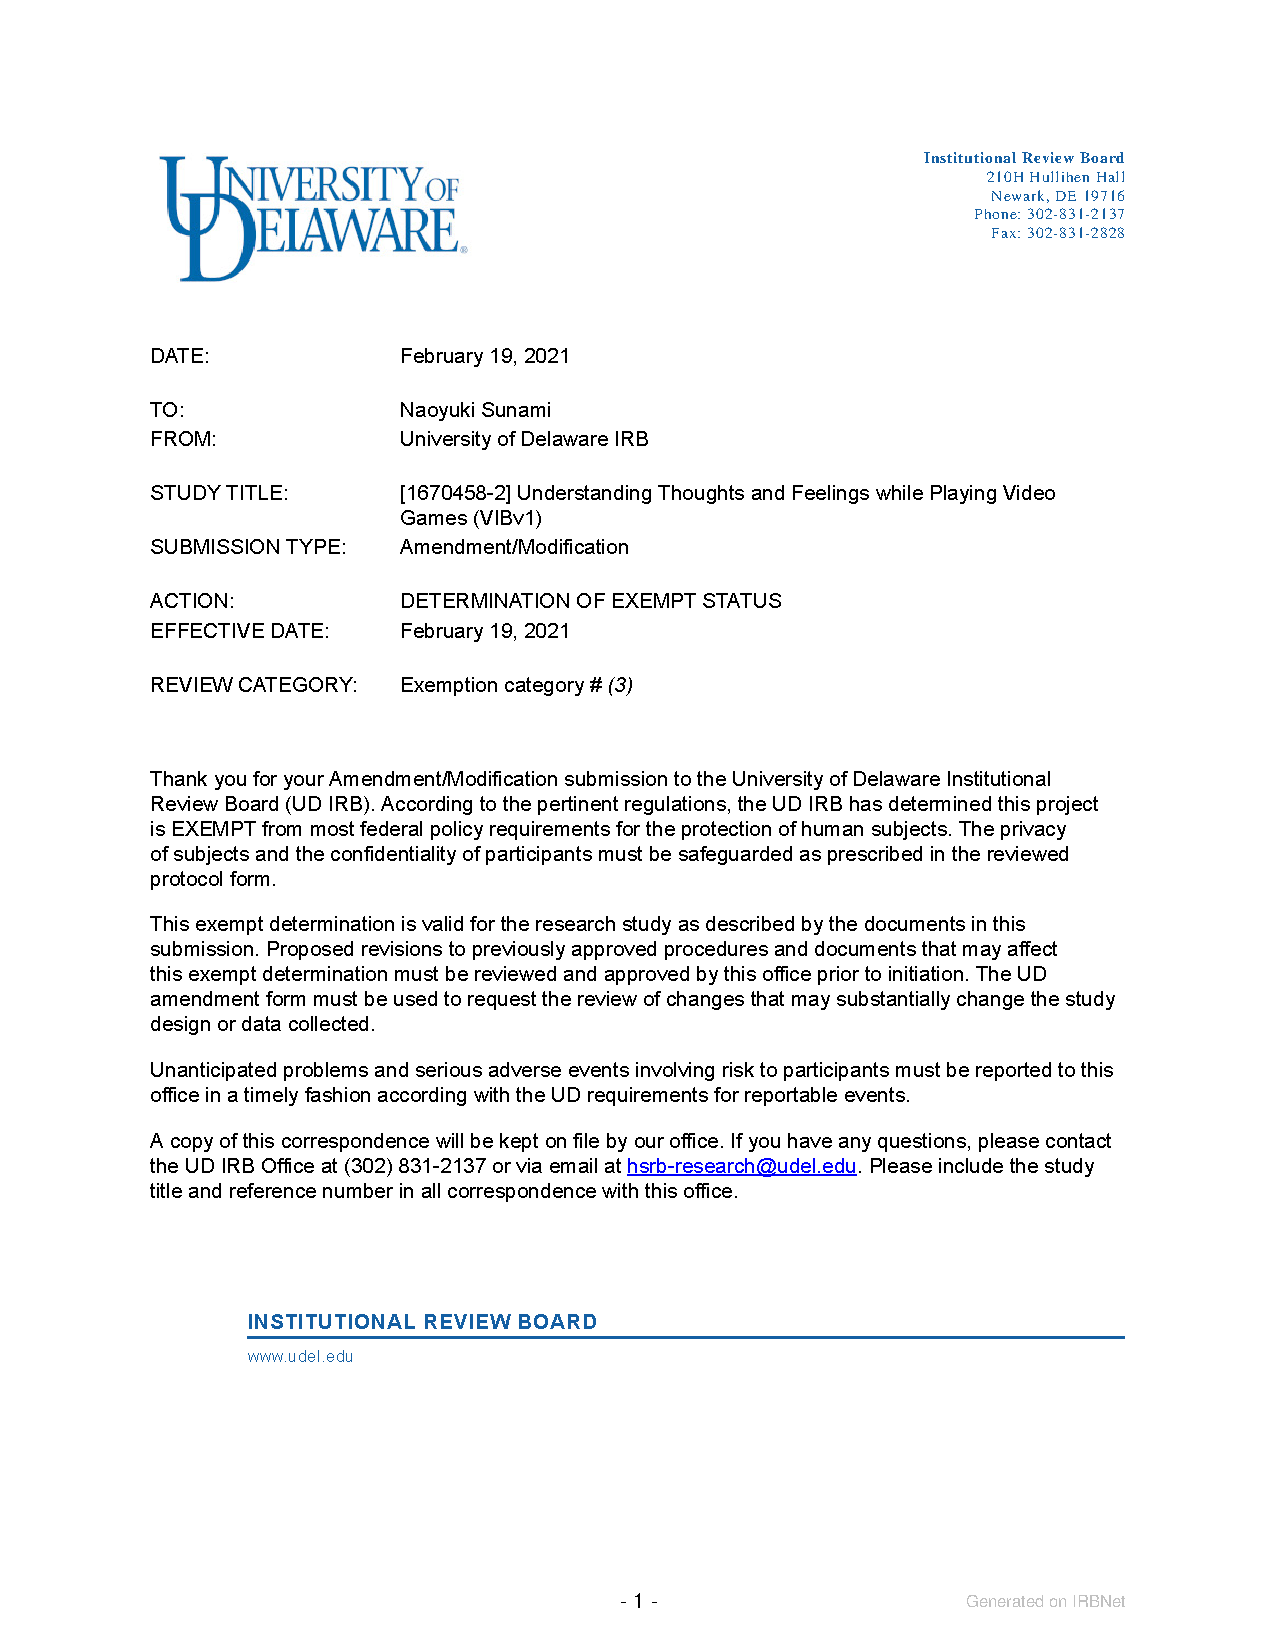
\includegraphics[width=1\linewidth]{pdf/IRB_letter2}

\chapter{Permissions}\label{permissions}

The current dissertation includes the following published work: Sunami, N., Nadzan, M. A., \&
Jaremka, L. M. (2019). The bi‐dimensional rejection taxonomy: Organizing
responses to interpersonal rejection along antisocial--prosocial and
engaged--disengaged dimensions. Social and Personality Psychology
Compass. \url{https://doi.org/10.1111/spc3.12497}. I have the right to self-archive this article to the institutional repository (under C.2.a in the attached copyright transfer agreement):

\begin{quote}
The right to self-archive the Accepted Version on: the Contributor's personal website; the Contributor's company/institutional repository or archive; Compliant SCNs; and not for profit subject-based repositories such as PubMed Central, all subject to an embargo period of 12 months for scientific, technical and medical (STM) journals and 24 months for social science and humanities (SSH) journals following publication of the Final Published Version.
\end{quote}

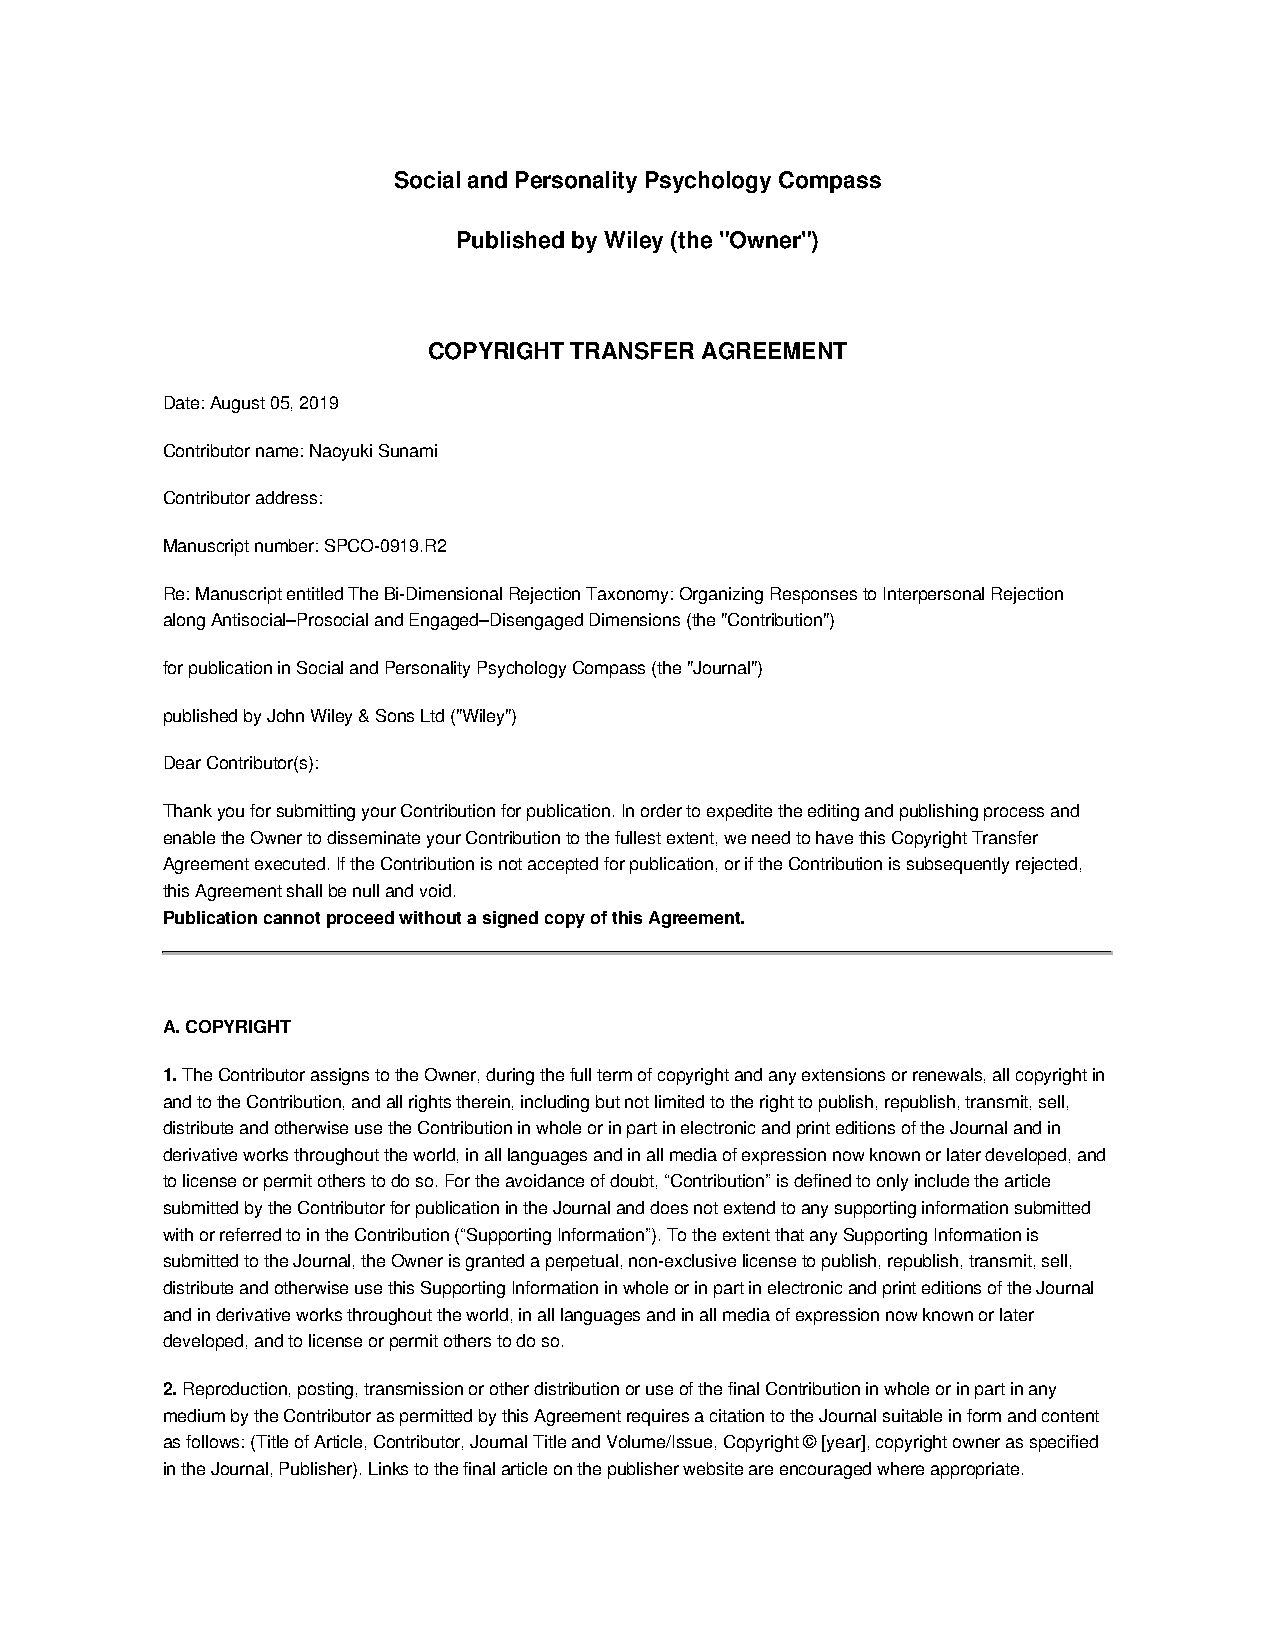
\includepdf[pages=-,nup=1,pagecommand={}]{pdf/copyright.pdf}

\end{document}
